% ============================================================
\documentclass[12pt,a4paper,oneside]{report}

% ---- Codificación y lengua ----
\usepackage[spanish,es-tabla]{babel}

% ---- Tipografía (LuaLaTeX — Times New Roman real) ----
\usepackage{fontspec}
\setmainfont{Times New Roman}
\usepackage{microtype}

% ---- Geometría de página ----
% UTEQ: izq 3 cm | sup 2.5 cm | inf 2.5 cm | der 2.5 cm
\usepackage[
top    = 2.5cm,
bottom = 2.5cm,
left   = 3cm,
right  = 2.5cm,
headheight = 0pt,
headsep    = 0pt,
footskip   = 1.2cm,
]{geometry}

% ---- Interlineado y párrafos ----
% UTEQ: interlineado 1.5 + doble espacio después de cada punto aparte
\usepackage{setspace}
\onehalfspacing
\setlength{\parskip}{\baselineskip}   % doble espacio entre párrafos (= 1 línea extra sobre el 1.5)
\setlength{\parindent}{0pt}

% ---- Gráficos ----
\usepackage{graphicx}
\usepackage{float}

% ---- Captions ----
\usepackage{caption}
\DeclareCaptionFormat{twoline}{\raggedright\textbf{#1#2}\par#3\par}
\captionsetup{
	format          = twoline,
	labelsep        = period,
	singlelinecheck = false,
	justification   = raggedright,
	font            = normalsize,
	skip            = 4pt,
}
\captionsetup[figure]{position=top}
\captionsetup[longtable]{position=top}

% ---- Numeración secuencial global (sin prefijo de capítulo) ----
\counterwithout{figure}{chapter}
\counterwithout{table}{chapter}
\counterwithout{equation}{chapter}

% ---- Pie de tabla ----
\newcommand{\tblnote}{%
	\vspace{-18pt}%
	\small\noindent\textbf{Fuente:} Investigación\\\quad\textbf{Elaborado por:} Autora%
	\vspace{12pt}%
}

% ---- TikZ y pgfplots ----
\usepackage{tikz}
\usetikzlibrary{positioning,shapes.geometric,arrows.meta,calc,babel}
\usepackage{pgfplots}
\pgfplotsset{compat=1.18}
\usepgfplotslibrary{polar}

% ---- Tablas ----
\usepackage{booktabs}
\usepackage{longtable}
\usepackage{array}
\usepackage{tabularx}
\usepackage{multirow}
\usepackage{colortbl}
\usepackage[table]{xcolor}
\renewcommand{\arraystretch}{1.2}
\setlength{\tabcolsep}{4pt}

% ---- Matemáticas ----
\usepackage{amsmath}
\usepackage{amssymb}

% ---- Hipervínculos ----
\usepackage[
colorlinks  = true,
linkcolor   = black,
citecolor   = black,
urlcolor    = blue,
bookmarks   = true,
bookmarksopen = true,
]{hyperref}

% ---- Bibliografía ----
\usepackage[numbers,sort&compress]{natbib}
\bibliographystyle{IEEEtran}

% ---- Encabezado/pie de página ----
% UTEQ: número en la parte inferior derecha; sin número impreso en portada
\usepackage{fancyhdr}
\pagestyle{fancy}
\fancyhf{}                              % limpia todo
\fancyfoot[R]{\small\thepage}          % número inferior derecho
\renewcommand{\headrulewidth}{0pt}     % sin línea de encabezado
\renewcommand{\footrulewidth}{0pt}

% Estilo para páginas de capítulo (plain) — también inferior derecho
\fancypagestyle{plain}{%
	\fancyhf{}
	\fancyfoot[R]{\small\thepage}
	\renewcommand{\headrulewidth}{0pt}
}

% ---- Títulos de secciones ----
\usepackage{titlesec}
\titleformat{\chapter}[block]
{\normalfont\large\bfseries\centering}{}{0pt}{\MakeUppercase}
\titlespacing*{\chapter}{0pt}{12pt}{12pt}
\titleformat{\section}[block]
{\normalfont\normalsize\bfseries}{\thesection}{1em}{}
\titlespacing*{\section}{0pt}{10pt}{6pt}
\titleformat{\subsection}[block]
{\normalfont\normalsize\bfseries}{\thesubsection}{1em}{}
\titlespacing*{\subsection}{0pt}{8pt}{4pt}
\titleformat{\subsubsection}[block]
{\normalfont\normalsize\bfseries}{}{0pt}{}
\titlespacing*{\subsubsection}{0pt}{6pt}{2pt}

% ---- Notas al pie ----
% UTEQ: Times New Roman 8 pt; no usar para referencias bibliográficas
\usepackage[hang,flushmargin]{footmisc}
\renewcommand{\footnotesize}{\fontsize{8pt}{10pt}\selectfont}

% ---- Listas ----
\usepackage{enumitem}
\setlist[itemize]{leftmargin=1.5cm,itemsep=2pt,parsep=0pt}
\setlist[enumerate]{leftmargin=1.5cm,itemsep=2pt,parsep=0pt}

% ---- Utilidades ----
\usepackage{rotating}
\usepackage{pdflscape}
\usepackage{url}
\usepackage{acronym}

% ---- Colores del proyecto ----
\definecolor{headblue}{RGB}{185,130,38}
\definecolor{grpgray}{RGB}{232,222,205}
\definecolor{barblue}{RGB}{70,130,180}
\definecolor{meanred}{RGB}{180,40,40}
\definecolor{threshgold}{RGB}{200,140,0}
\definecolor{gridgray}{RGB}{210,210,210}
\definecolor{hYellow}{RGB}{255,230,100}
\definecolor{hBlue}{RGB}{173,216,230}
\definecolor{aGreen}{RGB}{204,230,180}
\definecolor{barC}{RGB}{240,160,120}
\definecolor{grayBorder}{RGB}{160,160,160}

% ---- Macro para nombres de funciones en tablas ----
\newcommand{\fn}[1]{{\small\ttfamily\expandafter\fnbreak#1\_\relax}}
\def\fnbreak#1\_#2\relax{%
	#1\ifx\relax#2\relax\else\_\linebreak[0]\fnbreak#2\relax\fi}

% ---- Metadatos PDF ----
\hypersetup{
	pdftitle   = {Aplicación móvil con inteligencia artificial generativa
		para crear planes de ejercicios físicos personalizados para niños},
	pdfauthor  = {Chica Valfre, Valeska Sofia},
	pdfsubject = {Proyecto Tecnológico — Ingeniería de Software — UTEQ 2026},
	pdfkeywords= {inteligencia artificial generativa, actividad física infantil,
		aplicación móvil, FitKids, TDDM4IoTS},
}

%------ Separador de capítulo (página propia) ------
\newcommand{\capituloseparador}[2]{%
	\clearpage
	\thispagestyle{empty}
	\vspace*{\fill}
	\begin{center}
		{\large\bfseries CAPÍTULO #1}\\[1cm]
		{\large\bfseries #2}
	\end{center}
	\vspace*{\fill}
	\clearpage
	\thispagestyle{fancy}
	\refstepcounter{chapter}%
	\addcontentsline{toc}{chapter}{CAPÍTULO #1. #2}%
	\setcounter{section}{0}%
	\setcounter{figure}{0}%
	\setcounter{table}{0}%
}

% ============================================================
\begin{document}
	% ============================================================
	
	% ---- Portada ----
	\begin{titlepage}
		\begin{center}
			\vspace{1cm}
			
\includegraphics[width=5cm]{images/image3.jpeg}\\[0.75cm]
			{\large\bfseries UNIVERSIDAD TÉCNICA ESTATAL DE QUEVEDO}\\[0.1cm]
			{\normalsize \textbf{FACULTAD DE CIENCIAS DE LA COMPUTACIÓN}}\\[0.1cm]
			{\normalsize \textbf{CARRERA DE SOFTWARE}}\\[1.5cm]
			
			\begin{flushright}
				\begin{minipage}{0.35\textwidth}
					Trabajo de Integración Curricular previa la obtención del
					Grado Académico de Ingeniera de Software.
				\end{minipage}
			\end{flushright}
			\vspace{0.75cm}
			\textbf{PROYECTO TECNOLÓGICO:}\\[0.5cm]
			{``APLICACIÓN MÓVIL CON INTELIGENCIA ARTIFICIAL GENERATIVA PARA CREAR PLANES DE EJERCICIOS FÍSICOS PERSONALIZADOS PARA NIÑOS''}\\[1cm]
			
			\textbf{AUTORA:}
			
			CHICA VALFRE VALESKA SOFIA \\[1cm]
			
			\textbf{DIRECTOR DEL PROYECTO TECNOLÓGICO:}
				
			ING. GLEISTON CICERÓN GUERRERO ULLOA, PhD. \\
			[1.5cm]
			
			{\normalsize QUEVEDO — LOS RÍOS — ECUADOR}\\[0.3cm]
			{\normalsize 2026}
		\end{center}
	\end{titlepage}
	
	% ============================================================
	% PÁGINAS PRELIMINARES
	% ============================================================
	\pagenumbering{roman}
	\setcounter{page}{2}
	
	\begin{center}
		
\includegraphics[width=5cm]{images/image3.jpeg}\\[0.8cm]
		{\large\bfseries DECLARACIÓN DE AUTORÍA Y CESIÓN DE DERECHOS}\\[1.5cm]
	\end{center}
	\addcontentsline{toc}{chapter}{Declaración de autoría y cesión de derechos}
		Yo, Valeska Sofia Chica Valfre, declaro que la investigación aquí descrita es de mi autoría; que no ha sido previamente presentada para ningún grado o calificación profesional; y que he consultado las referencias bibliográficas que se incluyen en este documento.
		
		La Universidad Técnica Estatal de Quevedo puede hacer uso de los derechos correspondientes a este documento, según lo establecido por la Ley de Propiedad Intelectual, por su Reglamento y por la normatividad institucional vigente.
		\vspace{2cm}
		\begin{center}
			\rule{8cm}{0.5pt}\\
			Valeska Sofia Chica Valfre\\
			C.I: 1250328067
		\end{center}
		\clearpage
		
	\begin{center}
		
\includegraphics[width=5cm]{images/image3.jpeg}\\[0.8cm]
		{\large\bfseries INFORME FAVORABLE DEL DIRECTOR SOBRE LA CULMINACIÓN DEL TRABAJO DE INTEGRACIÓN CURRICULAR}\\[1.5cm]
	\end{center}
	\addcontentsline{toc}{chapter}{Informe favorable del director del trabajo de integración curricular}
		El suscrito, Gleiston Cicerón Guerrero Ulloa, Docente de la Universidad Técnica Estatal de Quevedo, certifica que la estudiante Valeska Sofia Chica Valfre realizó el Proyecto Tecnológico titulado ``Aplicación móvil con inteligencia artificial generativa para crear planes de ejercicios físicos personalizados para niños'', bajo mi tutoría, y que el mismo reúne los requisitos para ser defendido ante el tribunal que se designe para el efecto.
		\vspace{2cm}
		\begin{center}
			\rule{8cm}{0.5pt}\\
			Ing. Gleiston Cicerón Guerrero Ulloa, PhD.\\
			DIRECTOR DEL PROYECTO TECNOLÓGICO
		\end{center}
		\clearpage
		
	\begin{center}
		
\includegraphics[width=5cm]{images/image3.jpeg}\\[0.8cm]
		{\large\bfseries CERTIFICADO DEL REPORTE DE LA HERRAMIENTA DE PREVENCIÓN DE COINCIDENCIA Y/O PLAGIO ACADÉMICO}\\[1.5cm]
	\end{center}
	\addcontentsline{toc}{chapter}{Certificado de prevención de coincidencia y/o plagio}
		El suscrito, Gleiston Cicerón Guerrero Ulloa, mediante el presente cumple en presentar el informe del Proyecto Tecnológico titulado ``Aplicación móvil con inteligencia artificial generativa para crear planes de ejercicios físicos personalizados para niños'', elaborado por la egresada Valeska Sofia Chica Valfre, el cual presenta un porcentaje de similitud determinado por la herramienta de detección de coincidencias Turnitin.
		\vspace{2cm}
		\begin{center}
			\rule{8cm}{0.5pt}\\
			Ing. Gleiston Cicerón Guerrero Ulloa, PhD.\\
			DIRECTOR DEL PROYECTO TECNOLÓGICO
		\end{center}
		\clearpage
		
	\begin{center}
		
\includegraphics[width=5cm]{images/image3.jpeg}\\[0.25cm]
	\end{center}
	\addcontentsline{toc}{chapter}{Certificado de aprobación por tribunal de sustentación}
	\begin{center}
		\vspace{-0.25cm}
		\textbf{UNIVERSIDAD TÉCNICA ESTATAL DE QUEVEDO}\\
		\textbf{FACULTAD DE CIENCIAS DE LA COMPUTACIÓN}\\
		\textbf{CARRERA DE INGENIERÍA EN SOFTWARE}
		\\[0.75cm]
		\textbf{PROYECTO TECNOLÓGICO}
		\\[0.75cm]
		\textbf{TÍTULO:}
		
		{``Aplicación móvil con inteligencia artificial generativa
			para crear planes de ejercicios físicos personalizados para niños''}\\[0.25cm]
		{\normalsize Presentado al Consejo Directivo de la Facultad de Ciencias de la
			Computación como requisito previo a la obtención del título de Ingeniera de Software.}\\[0.25cm]
		{\normalsize Aprobado por:}\\[1.1cm]
		\rule{8cm}{0.5pt}\\
		{\normalsize PRESIDENTE DEL TRIBUNAL}\\
		{\normalsize Ing. Cristian Gabriel Zambrano Vega, PhD.}\\[1.1cm]
		\begin{tabular}{cc}
			\rule{6cm}{0.5pt} & \rule{6cm}{0.5pt} \\
			MIEMBRO DEL TRIBUNAL & MIEMBRO DEL TRIBUNAL \\
			Ing. Ariosto Eugenio Vicuña Pino, MSc. & Ing. Alex Rosendo Fiallos Barrionuevo, MSc.
		\end{tabular}\\[1cm]
		{\normalsize QUEVEDO — LOS RÍOS — ECUADOR}\\[0.3cm]
		{\normalsize 2026}
	\end{center}
	\clearpage
		
	\chapter*{AGRADECIMIENTO}
		A Dios, por darme fortaleza, sabiduría y constancia para culminar esta etapa importante de mi vida académica. Su guía me permitió afrontar cada desafío y mantenerme firme en el cumplimiento de este objetivo.
		
		Expreso mi más profundo agradecimiento a mi madre y a mi padre, quienes con su esfuerzo, sacrificio y apoyo incondicional me brindaron la oportunidad de alcanzar esta meta profesional. Gracias por sus valores, por su amor y por creer en mí en cada momento del camino.
		
		A mis hermanos, por acompañarme y brindarme ánimo en los momentos de mayor dificultad, convirtiéndose en un apoyo importante durante el desarrollo de este proyecto.
		
		A mi segunda madre, por su cariño, comprensión y respaldo incondicional, siendo una persona fundamental en mi crecimiento personal y académico.
		
		A mis amigos, por su apoyo, compañía y palabras de motivación durante este proceso, especialmente en los momentos de mayor presión y esfuerzo.
		
		Asimismo, agradezco a toda mi familia, quienes de una u otra manera estuvieron presentes brindándome apoyo y confianza para continuar adelante hasta culminar este trabajo de titulación. También expreso mi gratitud a mis docentes, quienes compartieron sus conocimientos, experiencias y orientaciones académicas, contribuyendo significativamente a mi formación profesional y al desarrollo de este proyecto tecnológico.
		\clearpage
		
	\chapter*{DEDICATORIA}
		Dedico este proyecto, en primer lugar, a mis padres, por su amor, esfuerzo y sacrificio incondicional a lo largo de toda mi vida. Gracias por ser mi mayor ejemplo de perseverancia y por brindarme siempre las herramientas necesarias para alcanzar mis sueños.
		
		A mis hermanos, por acompañarme en este camino y brindarme ánimo en los momentos más difíciles, recordándome siempre la importancia de seguir adelante. A mi segunda madre, por su cariño, comprensión y apoyo constante, siendo una persona fundamental en mi vida personal y académica.
		
		A mis amigos y familiares, quienes estuvieron presentes con palabras de aliento y motivación durante el desarrollo de este trabajo, aportando de distintas maneras para que este logro fuera posible. Dedico también este proyecto a todas las personas que confiaron en mí y me impulsaron a continuar luchando por mis sueños y objetivos profesionales.
		\clearpage
		
	\chapter*{RESUMEN}
		El sedentarismo infantil constituye una problemática global que compromete el desarrollo físico, emocional y social de los niños, reconocida por organismos internacionales de salud como uno de los principales desafíos para el bienestar infantil en la actualidad.
		
		Frente a esta problemática, se desarrolló FitKids, una aplicación móvil basada en inteligencia artificial generativa orientada a la creación de planes de ejercicios físicos personalizados para niños de 6 a 11 años. El sistema integra un motor de generación de rutinas mediante el modelo generativo Gemini de Google, complementado con un proceso de revisión y aprobación realizado por especialistas en actividad física infantil. Asimismo, incorpora una interfaz lúdica dirigida al niño y un módulo de supervisión parental con recordatorios y notificaciones configurables para el seguimiento de las rutinas.
		
		La construcción del sistema se realizó mediante la metodología TDDM4IoTS, desarrollada por Guerrero-Ulloa et al., la cual integra desarrollo guiado por pruebas, ingeniería dirigida por modelos y principios ágiles. La investigación se desarrolló bajo un enfoque aplicado y descriptivo, utilizando revisión bibliográfica y entrevistas dirigidas a especialistas y padres de familia para identificar las necesidades funcionales y no funcionales del sistema.
		
		La evaluación de FitKids se llevó a cabo con la participación de 15 niños de entre 6 y 11 años y 15 padres o tutores. Los resultados obtenidos evidenciaron un puntaje SUS de 81,17, correspondiente a la categoría ``excelente'' dentro de la escala normativa global de usabilidad~\cite{Bangor2008}. El modelo TAM registró valores promedio de 4,37 en utilidad percibida y 4,25 en facilidad de uso, ambos superiores al umbral de alta aceptación tecnológica~\cite{Venkatesh2003}. La tasa de adherencia observada y la validación profesional del contenido generado por IA respaldan la viabilidad de FitKids como una herramienta tecnológica para promover hábitos saludables y la actividad física en la infancia. Estos resultados confirman que la IA generativa, cuando se integra con validación profesional obligatoria y supervisión parental, constituye un enfoque técnicamente viable y contextualmente apropiado para producir contenido de ejercicio seguro y personalizado para niños en entornos domésticos.
		
		Los resultados confirman la viabilidad técnica y la aceptación inicial del sistema como herramienta de apoyo para la promoción de hábitos activos en la infancia.
		
		\vspace{0.5cm}
		\noindent\textbf{Palabras clave:} inteligencia artificial generativa, actividad física infantil, aplicación móvil, personalización de ejercicios, sedentarismo infantil.
		\clearpage
		
	\chapter*{ABSTRACT}
		Childhood sedentary behavior is a growing global problem that affects the physical, emotional, and social development of children, recognized by international health organizations as one of the main challenges to child well-being today.
		
		In response to this problem, FitKids was developed: a mobile application based on generative artificial intelligence aimed at creating personalized physical exercise plans for children aged 6 to 11 years. The system integrates a routine generation engine using Google's Gemini generative model, complemented by a review and approval process carried out by specialists in childhood physical activity. It also incorporates a playful interface designed for the child and a parental supervision module with configurable reminders and notifications for routine monitoring.
		
		The system was built using the TDDM4IoTS methodology, developed by Guerrero-Ulloa et al., which integrates test-driven development, model-driven engineering, and agile principles. The research was conducted under an applied and descriptive approach, using literature review and interviews with specialists and parents to identify the functional and non-functional requirements of the system.
		
		FitKids was evaluated with 15 children aged 6 to 11 years and 15 parents or guardians over a four-week period. Results showed a System Usability Scale (SUS) score of 81.17, classified as ``excellent'' according to the normative global usability scale~\cite{Bangor2008}. The Technology Acceptance Model (TAM) recorded mean scores of 4.37 for perceived usefulness and 4.25 for ease of use, both exceeding the high technological acceptance threshold~\cite{Venkatesh2003}. The observed adherence rate and the professional validation of AI-generated content support the viability of FitKids as a technological tool for promoting healthy habits and physical activity in childhood. These results confirm that generative AI, when integrated with mandatory professional validation and parental supervision, constitutes a technically viable and contextually appropriate approach for producing safe, personalized exercise content for children in home settings.
		
		
		\vspace{0.5cm}
		\noindent\textbf{Keywords:} generative artificial intelligence, childhood physical activity, mobile application, personalized exercise plans, childhood sedentary behavior.
		\clearpage
		
	\chapter*{CÓDIGO DUBLÍN}
		\begin{table}[H]
			\centering
			\caption{Metadatos Dublin Core del proyecto FitKids}
			\begin{tabular}{|p{4.5cm}|p{9.5cm}|}
				\hline
				\textbf{Campo} & \textbf{Contenido}\\
				\hline
				Título      & Aplicación móvil con inteligencia artificial generativa para crear planes de ejercicios físicos personalizados para niños\\\hline
				Creador     & Chica Valfre, Valeska Sofia\\\hline
				Tema        & Inteligencia artificial generativa; actividad física infantil; sedentarismo; aplicación móvil; personalización de ejercicios\\\hline
				Descripción & Desarrollo de FitKids, aplicación móvil basada en el modelo generativo Gemini que genera rutinas de ejercicio personalizadas para niños de 6 a 11 años, con validación de especialistas y supervisión parental. Evaluada con SUS\,=\,81,17, TAM-UP\,=\,4,37 y TAM-FU\,=\,4,25 sobre una muestra de 15 niños y 15 padres durante cuatro semanas.\\\hline
				Editor      & Universidad Técnica Estatal de Quevedo, Facultad de Ciencias de la Computación\\\hline
				Colaborador & Guerrero Ulloa, Gleiston Cicerón (Director)\\\hline
				Fecha       & 2026\\\hline
				Tipo        & Texto — Proyecto Tecnológico de Titulación\\\hline
				Formato     & application/pdf\\\hline
				Idioma      & es (Español)\\\hline
				Cobertura   & Quevedo, Los Ríos, Ecuador\\\hline
				Derechos    & Universidad Técnica Estatal de Quevedo\\
				\hline
			\end{tabular}
		\end{table}
	\clearpage
	
	% ---- Índices ----
	\tableofcontents\clearpage
	\listoftables\clearpage
	\listoffigures\clearpage
	
	% ============================================================
	% CUERPO PRINCIPAL
	% ============================================================
	\pagenumbering{arabic}
	\setcounter{page}{1}
	% Dublin code table is in main.tex
	\chapter*{INTRODUCCIÓN}
	\addcontentsline{toc}{chapter}{INTRODUCCIÓN}
		En la actualidad, el sedentarismo infantil se ha convertido en una problemática relevante a nivel mundial, asociada a cambios en los estilos de vida, al incremento del tiempo frente a pantallas y a la disminución de la actividad física en edades tempranas~\cite{Guthold2020}. Esta situación repercute negativamente en el desarrollo físico, emocional y social de los niños, incrementando el riesgo de enfermedades como el sobrepeso y la obesidad, así como otros trastornos que afectan su bienestar integral~\cite{Musa2022}. Como se documenta en el Capítulo~I, la brecha entre los niveles recomendados de actividad física y los niveles reales observados en niños y adolescentes es significativa a nivel mundial, situación que posiciona al sedentarismo como un problema de salud pública prioritario~\cite{Bull2020}.
	
		El desarrollo tecnológico y la expansión del uso de dispositivos móviles han transformado la manera en que los niños interactúan con su entorno, influyendo tanto de forma positiva como negativa en sus hábitos cotidianos. Si bien el uso excesivo de la tecnología se ha vinculado al aumento del sedentarismo~\cite{Musa2022}, también se reconoce su potencial como herramienta para promover estilos de vida activos cuando es utilizada de manera adecuada~\cite{Direito2017}. Para este contexto, las aplicaciones móviles orientadas a la salud se presentan como una alternativa accesible para fomentar la actividad física, siempre que integren estrategias de motivación, personalización y seguimiento acordes a las características de los usuarios infantiles~\cite{Zhu2024}.
	
		La incorporación de inteligencia artificial en aplicaciones móviles ha permitido el desarrollo de soluciones orientadas a la personalización de servicios, adaptando contenidos y recomendaciones a las necesidades específicas de cada usuario. En el ámbito de la actividad física, evidencia empírica reciente demuestra que la inteligencia artificial generativa facilita la creación dinámica de planes de ejercicio, considerando variables como la edad, el nivel de actividad y las preferencias individuales, superando así la rigidez de las rutinas genéricas tradicionales~\cite{Pareek2025}. Sin embargo, diversos estudios evidencian que muchas aplicaciones existentes aún ofrecen rutinas estandarizadas, con escasas opciones de adaptación y limitados mecanismos de seguimiento, lo que reduce su impacto a largo plazo~\cite{Direito2017,Zhu2024}. Ante esta problemática surge la siguiente pregunta de investigación que guía este trabajo: ¿Qué estrategias pueden implementarse para reducir el sedentarismo infantil y promover la actividad física, considerando la influencia de la tecnología, la falta de estímulos y la ausencia de mecanismos de seguimiento?~\cite{Bull2020}.
	
		Los padres o representantes legales desempeñan un rol fundamental en la promoción de hábitos saludables en la infancia. Sin embargo, no siempre cuentan con herramientas tecnológicas que les permitan supervisar, evaluar y ajustar de manera informada la actividad física de sus hijos~\cite{VegaDiaz2023}. La falta de sistemas de monitoreo claros y de retroalimentación adecuada dificulta la creación de hábitos sostenibles, lo que evidencia la necesidad de soluciones que integren la participación familiar en el proceso de promoción de la actividad física~\cite{Direito2017}.
		
		Para dar respuesta a esta problemática, el objetivo general del presente trabajo consistió en desarrollar una aplicación móvil (denominada FitKids) basada en inteligencia artificial generativa para diseñar y gestionar planes de ejercicios personalizados, dirigida a niños, con el propósito de fomentar hábitos saludables, mejorar su bienestar físico y promover su desarrollo integral. Para alcanzar esta meta, se han delineado objetivos específicos (detallados en la subsección~1.2 del documento), los cuales abarcan: el análisis de funcionalidades necesarias mediante investigación y entrevistas, el desarrollo de interfaces y métricas estadísticas, la generación de planes de ejercicio seguros mediante IA, y el diseño de sistemas de recordatorios para padres y niños.
	
		Como aporte diferenciador y para garantizar la calidad y robustez de la solución, la construcción del sistema se rigió bajo la metodología TDDM4IoTS (\textit{Test-Driven Development Methodology for IoT Systems})~\cite{GuerreroUlloa2024}. Este enfoque metodológico, estructurado en fases iterativas desde el análisis preliminar hasta el mantenimiento, permite una integración eficiente entre el desarrollo de las interfaces (React y React Native), la lógica del sistema (FastAPI) y la integración de modelos de inteligencia artificial generativa (Gemini), asegurando que la herramienta tecnológica responda a las necesidades reales de sus usuarios finales.
	
	\capituloseparador{I}{MARCO CONTEXTUAL DEL PROYECTO TECNOLÓGICO}
	\label{marcontextual}
		\section{Problema de investigación}
			El Capítulo~I contextualiza el problema central del proyecto: la brecha entre los niveles recomendados de actividad física y los que la población infantil alcanza en la práctica. Las secciones siguientes profundizan en las dimensiones específicas de esa brecha --- clínica, familiar, tecnológica y de monitoreo --- que justifican la necesidad de una solución personalizada, supervisada e integrada como FitKids.

			\subsection{Planteamiento del problema}
				Desde una perspectiva clínica, la inactividad física en la infancia no es un fenómeno aislado: se articula con factores de riesgo cardiometabólico, musculoesquelético y psicológico que se consolidan con el tiempo~\cite{Wilhite2023}. Investigaciones con seguimiento longitudinal demuestran que la combinación de baja actividad física, conducta sedentaria elevada y sueño insuficiente produce los peores perfiles de salud física, psicológica y académica en niños y adolescentes de 5 a 17 años, con efectos más marcados cuando la conducta sedentaria se define como tiempo de pantalla frente a otras formas de inactividad~\cite{Wilhite2023}. Esta evidencia subraya que el sedentarismo no es un problema unidimensional: exige intervenciones que actúen simultáneamente sobre la motivación, la personalización del ejercicio y el entorno familiar~\cite{Hesketh2017}.
				
				En el ámbito comunitario y familiar, el problema se manifiesta a través del poco tiempo disponible de los padres y de la falta de programas que promuevan de manera atractiva la actividad física en los niños~\cite{Hesketh2017}. Muchas familias no cuentan con espacios adecuados para el ejercicio, y las alternativas existentes ---como programas televisivos o aplicaciones genéricas--- no siempre resultan interesantes ni se ajustan a los gustos y necesidades de cada niño~\cite{VegaDiaz2023}. Así, por ejemplo, un niño interesado en el baloncesto puede recibir rutinas que no consideran sus preferencias, mientras que otro con asma puede enfrentarse a ejercicios poco apropiados para su condición. Esta desconexión genera frustración tanto en los niños como en sus padres y dificulta la construcción de hábitos saludables y sostenibles en el tiempo.
				
				A nivel individual, cada niño enfrenta desafíos específicos que pueden abordarse mediante la actividad física, la cual fortalece el desarrollo motor y favorece su crecimiento integral~\cite{Wilhite2023}. Por el contrario, la falta de ejercicio se traduce en debilidad muscular, menor coordinación motriz y baja resistencia, lo que impacta negativamente en su desempeño cotidiano~\cite{Musa2022}. A esto se suma la ausencia de estímulos que hagan del movimiento una experiencia divertida y motivadora: la evidencia muestra que las intervenciones mHealth que incorporan elementos de gamificación ---logros, recompensas, retroalimentación visual inmediata--- aumentan significativamente la participación y la adherencia a la actividad física frente a programas sin estos componentes~\cite{Xu2022}. Sin embargo, estos mecanismos no se encuentran ampliamente disponibles ni adaptados al contexto de los niños en edad escolar~\cite{Zhu2024}.
				
				Tampoco existen, de manera generalizada, sistemas claros para registrar y monitorear el progreso de los niños en la actividad física. No siempre se recopilan datos sobre el tiempo que dedican al ejercicio, los tipos de actividades que realizan o las mejoras en habilidades como la coordinación y la resistencia~\cite{Direito2017}. Sin esta información, resulta difícil determinar si están avanzando adecuadamente o si es necesario ajustar las rutinas. A ello se suma la falta de retroalimentación positiva: sin animaciones, sonidos o mensajes motivadores, el ejercicio puede percibirse como una tarea monótona y poco atractiva, lo que disminuye el entusiasmo y favorece el abandono de la actividad física~\cite{Xu2022}.
				
				En síntesis, el rol parental en la promoción de la actividad física infantil es determinante, pero con frecuencia está limitado por la falta de herramientas que faciliten el acompañamiento informado. La meta-análisis de Yao y Rhodes~\cite{Yao2015} ---que sintetiza 115 estudios--- confirma que el apoyo parental es el correlato más consistente de la actividad física en niños y adolescentes, con mayor efecto que el modelado conductual. Pese a ello, muchos padres no disponen de herramientas que les permitan monitorear y ajustar de forma informada las rutinas de sus hijos: no siempre reciben notificaciones cuando el niño no cumple con las metas mínimas de actividad, ni cuentan con opciones flexibles para modificar los planes de ejercicio conforme a las necesidades del menor~\cite{Hesketh2017}. Esta carencia dificulta garantizar que las actividades sean seguras, efectivas y verdaderamente adaptadas a cada niño.

				\subsubsection{Diagnóstico}
					En la actualidad, muchos niños dedican gran parte de su tiempo libre a actividades sedentarias vinculadas al uso de dispositivos electrónicos, como teléfonos móviles, tabletas, videojuegos y televisión. La evidencia indica que el tiempo de pantalla excesivo se asocia de forma dosis-respuesta con componentes del síndrome metabólico ---incluidas la obesidad, la hipertensión, la dislipidemia y la resistencia a la insulina--- en población adolescente~\cite{Musa2022}, y que estas asociaciones son independientes del nivel total de actividad física realizada. Aunque existen recomendaciones internacionales que sugieren un mínimo de actividad física diaria~\cite{Bull2020}, una proporción importante de niños no alcanza estos niveles, lo que evidencia una brecha entre lo recomendado y lo que ocurre en la práctica~\cite{Guthold2020}.
					
					En el entorno familiar se observa, además, que los padres no siempre cuentan con el tiempo, la orientación o los recursos necesarios para organizar actividades físicas de forma constante y adecuada a la edad, condición física e intereses de sus hijos~\cite{VegaDiaz2023}. Las rutinas se improvisan o dependen de la disponibilidad del adulto, y en muchos casos no se dispone de criterios claros para definir la intensidad, duración o tipo de ejercicios más apropiados~\cite{Hesketh2017}. A ello se suma que las alternativas tecnológicas existentes ---videos genéricos, programas estandarizados o aplicaciones con contenidos poco interactivos--- no siempre resultan atractivas para los niños ni consideran sus preferencias específicas, lo que deriva en desinterés y abandono temprano~\cite{Zhu2024}.
					
					Desde el punto de vista tecnológico, se dispone de aplicaciones y plataformas orientadas a la actividad física, pero muchas de ellas ofrecen planes poco flexibles, con escasas opciones de personalización y sin un seguimiento detallado del progreso del niño~\cite{Direito2017}. En numerosos casos, no se registran de forma sistemática variables como el tiempo dedicado al ejercicio, el tipo de actividad realizada o la evolución en habilidades motoras, ni se incorporan mecanismos de retroalimentación positiva sostenida ---como logros, mensajes motivadores o dinámicas lúdicas--- que refuercen la constancia~\cite{Xu2022}. Esto limita el potencial de la tecnología para transformar la actividad física en una experiencia atractiva, adaptada y mantenida en el tiempo~\cite{Zhu2024}.
					
				\subsubsection{Pronóstico}
					Si la situación de sedentarismo infantil continúa sin intervenciones específicas ni apoyo de herramientas tecnológicas adecuadas, en los próximos años se incrementará la prevalencia de sobrepeso y obesidad en la población infantil. También aumentarán problemas relacionados, como dificultades respiratorias, alteraciones metabólicas y menor rendimiento físico, afectando su salud y calidad de vida~\cite{Wilhite2023}.
					
					Si no se desarrollan soluciones que apoyen a las familias, los padres continuarán teniendo dificultades para organizar rutinas de ejercicio adaptadas a la edad, intereses y condiciones particulares de sus hijos~\cite{Yao2015}. La ausencia de sistemas de registro y retroalimentación limitará su capacidad para evaluar la suficiencia y efectividad de las actividades físicas realizadas~\cite{Direito2017}.
					
					Ante este panorama, la ausencia de herramientas tecnológicas pertinentes que ofrezcan personalización, seguimiento parental y validación profesional del contenido generado constituye una brecha crítica que, de no atenderse, perpetuará las consecuencias descritas en el diagnóstico y profundizará la inequidad en el acceso a intervenciones de salud infantil basadas en evidencia~\cite{Hesketh2017}.

			\subsection{Formulación del problema}
				
				\begin{itemize}
					\item ¿Qué estrategias pueden implementarse para reducir el sedentarismo infantil y promover la actividad física, considerando la influencia de la tecnología, la falta de estímulos y la ausencia de mecanismos de seguimiento?
				\end{itemize}

			\subsection{Sistematización del problema}

				\begin{itemize}
					\item ¿Cuáles son las características y funcionalidades que deben incorporarse para motivar a los niños a realizar actividad física de manera regular?
					\item ¿Cuáles son las características necesarias en las interfaces de una aplicación móvil para asegurar una experiencia intuitiva y atractiva, que incluya gráficas estadísticas dinámicas y claras para el seguimiento de la actividad física en los niños?
					\item ¿Cómo se puede obtener rutinas de ejercicio adaptados al contexto, capacidades y necesidades específicas de los niños, que garanticen que son actividades seguras, motivadoras y divertidas?
					\item ¿Qué tipo de recordatorios y retroalimentación pueden incentivar la práctica constante de ejercicio en los niños, además de mantener informados a sus padres?
				\end{itemize}
				
		\section{Objetivos}
			\label{objectives}
			La inactividad física en la infancia representa uno de los desafíos de salud pública más urgentes de la última década: más del 81\% de los adolescentes a nivel global no cumple con las recomendaciones mínimas de actividad física moderada a vigorosa establecidas por la OMS~\cite{Guthold2020}, y las tasas no han mejorado de forma significativa en los últimos quince años a pesar de múltiples iniciativas institucionales. Frente a este escenario, la tecnología móvil ofrece un canal de intervención accesible, escalable y adaptable que puede llegar a poblaciones que raramente acceden a programas presenciales de actividad física~\cite{Direito2017}. FitKids surge como respuesta a esta brecha, con el propósito de aprovechar la inteligencia artificial generativa para producir planes de ejercicio personalizados que sean seguros, motivadores y sostenibles en el tiempo para niños de 6 a 11 años. Los objetivos que orientan su desarrollo se presentan a continuación.
			
			\subsection{Objetivo general}
			\label{objgen}
				El objetivo general de FitKids se inscribe en la necesidad documentada de desarrollar soluciones digitales que vayan más allá del catálogo estático de ejercicios y que respondan a las características individuales de cada niño. Mientras que la mayoría de las aplicaciones comerciales disponibles ofrecen rutinas predefinidas sin adaptación dinámica al perfil del usuario~\cite{Schoeppe2017}, FitKids propone un enfoque radicalmente diferente: utilizar la capacidad generativa de modelos de lenguaje de gran escala para producir planes únicos, revisados por especialistas antes de llegar al niño, y entregados a través de una interfaz diseñada específicamente para su grupo etario~\cite{Hourcade2015}. Este enfoque integrado ---personalización, validación clínica y diseño centrado en el niño--- es el núcleo del objetivo general que se enuncia a continuación.
				
				\begin{itemize}
					\item Desarrollar una aplicación móvil basada en inteligencia artificial generativa para diseñar y gestionar planes de ejercicios personalizados, dirigida a niños, con el propósito de fomentar hábitos saludables, mejorar su bienestar físico y promover su desarrollo integral desde la infancia.
				\end{itemize}
				
			\subsection{Objetivos específicos}
				\label{objesp}
				Los objetivos específicos operacionalizan el objetivo general en cuatro líneas de acción concretas que corresponden a las fases de investigación, desarrollo, implementación y evaluación del sistema. Cada línea responde a una limitación identificada en la literatura: la ausencia de diagnóstico previo de las necesidades reales de padres y especialistas~\cite{Zhang2024}, la falta de interfaces adaptadas al grupo etario de 6 a 11 años~\cite{Hourcade2015}, la carencia de mecanismos de personalización dinámica basados en IA en aplicaciones infantiles existentes~\cite{Sengar2024}, y la insuficiente incorporación de herramientas de retroalimentación y recordatorio que sostengan la adherencia a largo plazo~\cite{WangGamif2025}.
				
				\begin{itemize}
					\item Analizar las características y funcionalidades necesarias para fomentar la actividad física en los niños, a través de una revisión de la literatura y la realización de entrevista a expertos y padres de familia.
					\item Desarrollar todos los interfaces y módulos de la aplicación móvil, incluyendo el registro de ejercicios y la visualización del progreso infantil mediante gráficas estadísticas dinámicas y claras, asegurando una interfaz intuitiva, atractiva y funcional.
					\item Generar planes de ejercicio adaptados al contexto, capacidades y necesidades específicas de los niños, utilizando algoritmos de inteligencia artificial generativa que garanticen actividades seguras, motivadoras y divertidas.
					\item Diseñar los recordatorios y la retroalimentación que mejoren la adherencia a la práctica constante de ejercicio en los niños, mientras los padres se mantienen informados.
				\end{itemize}

		\section{Justificación}
		\label{sec:just}
			El sedentarismo infantil, cuya magnitud epidemiológica se documenta en el apartado 1.1.1, genera consecuencias directas sobre la población objetivo del presente proyecto, incrementando el riesgo de obesidad, enfermedades cardiovasculares, ansiedad y baja autoestima desde edades tempranas~\cite{Wilhite2023}.
			
			Los beneficiarios directos de este proyecto son los niños, quienes podrán acceder a planes de ejercicios físicos personalizados que contribuyan a mejorar su bienestar físico y emocional, fomentando hábitos saludables desde edades tempranas~\cite{Xu2022}. De esa manera, los padres o representantes legales se benefician al contar con una herramienta tecnológica que les permite supervisar, monitorear y ajustar las rutinas de actividad física de sus hijos de manera informada y segura~\cite{Yao2015}.
			
			De forma indirecta, este proyecto beneficia a profesionales de la salud, educadores y a la comunidad en general, al ofrecer una solución tecnológica que puede apoyar estrategias de prevención del sedentarismo infantil. Desde una perspectiva académica y tecnológica, la propuesta aporta al desarrollo de soluciones basadas en inteligencia artificial generativa aplicadas al ámbito de la salud infantil, evidenciando su utilidad en la personalización de servicios y en la promoción del bienestar integral~\cite{Pareek2025}.
			
			Actualmente existen barreras importantes que dificultan la actividad física en los niños. Entre ellas se encuentran el uso excesivo de pantallas, la falta de motivación, la ausencia de seguimiento adecuado y la carencia de políticas públicas efectivas~\cite{Hesketh2017}. También faltan estímulos y mecanismos de monitoreo que ayuden a generar hábitos sostenibles~\cite{Zhu2024}. Ante esta situación, surge la necesidad de soluciones innovadoras que integren tecnología y personalización para superar dichas limitaciones~\cite{Direito2017}.
			
			La propuesta de una aplicación móvil basada en inteligencia artificial generativa responde a esta necesidad. Esta herramienta permite a los padres registrar información clave sobre sus hijos ---como edad, intereses y condiciones médicas--- para generar rutinas de ejercicio personalizadas. Además, incluye recordatorios, estadísticas de progreso y retroalimentación positiva, como animaciones y mensajes motivadores, que convierten el ejercicio en una experiencia más divertida y atractiva. También posibilita que los padres monitoreen y ajusten las rutinas, garantizando que las actividades sean seguras, efectivas y adaptadas a cada niño.
			
			Esta propuesta se alinea con varios Objetivos de Desarrollo Sostenible (ODS) de las Naciones Unidas, lo que refuerza su relevancia. Contribuye al \textbf{ODS 3: Salud y Bienestar}, al fomentar la actividad física en los niños y ayudar a prevenir problemas como obesidad y ansiedad, mejorando su calidad de vida y promoviendo hábitos saludables desde una edad temprana~\cite{UN2015}. Asimismo, apoya el \textbf{ODS 10: Reducción de las Desigualdades}, al ser accesible desde distintos contextos y adaptarse a las necesidades de cada niño, eliminando barreras económicas y geográficas y promoviendo la igualdad de oportunidades~\cite{UN2015}. También impulsa el \textbf{ODS 9: Industria, Innovación e Infraestructura}, al integrar inteligencia artificial y tecnología móvil en una solución innovadora orientada al bienestar infantil y al desarrollo tecnológico sostenible~\cite{UN2015}.
			
			La aplicabilidad de este proyecto radica en su capacidad para integrar tecnología avanzada con estrategias de personalización y monitoreo. La personalización de rutinas, los recordatorios y la retroalimentación positiva contribuyen a que las actividades sean seguras, efectivas y motivadoras, reduciendo barreras económicas y geográficas y ofreciendo una herramienta accesible y sostenible que fomenta hábitos saludables desde la infancia~\cite{Zhu2024,Direito2017}.
			
			El proyecto contribuye a prevenir problemas como obesidad y ansiedad, mejora el bienestar físico y emocional de los niños y fortalece la educación física, al tiempo que promueve la participación activa de los padres y genera conciencia sobre la importancia de la actividad física. Desde una perspectiva científica, permite evaluar la efectividad de la inteligencia artificial generativa en la personalización de rutinas, abriendo nuevas posibilidades en el diseño de herramientas tecnológicas para la salud~\cite{Pareek2025}.
			
			Por lo tanto, la solución propuesta tiene el potencial de influir en políticas públicas al demostrar cómo la tecnología puede abordar problemas de salud infantil. Esto puede inspirar programas gubernamentales que integren herramientas tecnológicas para fomentar hábitos saludables. La viabilidad del proyecto se respalda en el uso de tecnologías accesibles, metodologías de monitoreo y estrategias de motivación basadas en evidencia científica, lo que representa una solución innovadora y de alto impacto para combatir el sedentarismo infantil~\cite{Guthold2020,Bull2020}.

	\capituloseparador{II}{MARCO TEÓRICO DEL PROYECTO TECNOLÓGICO}
	\label{marcoteorico}
	
		\section{Marco conceptual}
			En esta sección se exponen los conceptos fundamentales, que servirán como base teórica para comprender y orientar el diseño y desarrollo de la aplicación.
			
			\subsection{Inteligencia Artificial Generativa}
				La inteligencia artificial generativa, una tecnología que está revolucionando la forma en que se crean soluciones personalizadas en diferentes campos. Esta tecnología posee un gran potencial, especialmente en el desarrollo de aplicaciones orientadas a mejorar la salud y el bienestar de los niños.

				\subsubsection{Definición y características de la inteligencia artificial generativa}
					La IA generativa se define como el conjunto de técnicas de aprendizaje automático que permiten a un modelo aprender la distribución estadística de un conjunto de datos de entrenamiento y, a partir de ella, producir instancias nuevas coherentes con esa distribución~\cite{Cao2023}. Entre los modelos más representativos se encuentran los modelos de lenguaje de gran escala (LLM, por sus siglas en inglés), como los de la familia GPT y Gemini de Google, y los modelos de difusión para generación de imágenes. Sus características distintivas son tres: (1) \textit{capacidad generativa}, que le permite producir contenido que no existía previamente en los datos de entrenamiento; (2) \textit{adaptabilidad contextual}, que le permite incorporar instrucciones en lenguaje natural ---conocidas como \textit{prompts}--- para orientar la generación hacia objetivos específicos; y (3) \textit{escalabilidad}, que le permite operar sobre volúmenes masivos de datos con tiempos de respuesta apropiados para aplicaciones en tiempo real~\cite{Sengar2024}. En el contexto de FitKids, estas características se aprovechan para generar rutinas de ejercicio únicas a partir de variables de entrada como la edad, los intereses deportivos y las condiciones médicas de cada niño, garantizando que ningún usuario reciba exactamente el mismo plan que otro.
					
					La distinción entre la IA generativa y los enfoques de IA clásica resulta determinante para entender el valor diferencial de FitKids. Los sistemas de IA tradicionales, como los clasificadores de actividad física o los modelos de recomendación por filtrado colaborativo, operan dentro de un espacio de clases o patrones previamente aprendidos y no pueden producir contenido fuera de ese espacio~\cite{Cao2023}. La IA generativa, en cambio, no está limitada a un catálogo predefinido: puede sintetizar un plan de ejercicios que nunca antes ha existido, combinando de forma novedosa tipos de movimiento, duraciones, niveles de intensidad y elementos lúdicos en función del perfil específico del usuario~\cite{Sengar2024}. La Tabla~\ref{tab:ia_comparativa} sintetiza esta comparación en el contexto de las aplicaciones de salud infantil.
					
					\begin{table}[H]
						\centering
						\caption[Comparación entre inteligencia artificial tradicional e inteligencia artificial generativa]{Comparación entre inteligencia artificial tradicional e inteligencia artificial generativa en el contexto de aplicaciones de salud infantil}
						\label{tab:ia_comparativa}
						
						\begin{tabular}{p{4.2cm} p{5.1cm} p{5.2cm}}
							\hline
							\textbf{Dimensión} & \textbf{IA tradicional} & \textbf{IA generativa} \\
							\hline
							Tipo de salida & Clasificaciones o predicciones sobre datos existentes & Contenido nuevo y original (textos, planes, imágenes) \\
							
							Personalización & Estática: basada en reglas predefinidas & Dinámica: generada en tiempo real según el perfil del usuario \\
							
							Flexibilidad & Limitada al espacio de clases entrenadas & Alta: puede generar variantes ilimitadas \\
							
							Interacción & Unidireccional (entrada → salida fija) & Conversacional: acepta instrucciones en lenguaje natural \\
							
							Ejemplo en salud infantil & Clasificar nivel de actividad física & Generar una rutina personalizada para un niño de 8 años con asma \\
							\hline
						\end{tabular}
					\end{table}
					\tblnote
				
				\subsubsection{Aplicaciones de la inteligencia artificial generativa en la personalización de servicios}
					La IA generativa ha demostrado su capacidad para transformar la prestación de servicios en múltiples dominios, al adaptar contenidos y recomendaciones a las necesidades específicas de cada usuario de manera automática y escalable~\cite{Sengar2024}. En el ámbito de la salud, una revisión narrativa sistemática publicada en \textit{JMIR Medical Informatics} identifica que los modelos generativos están siendo empleados para apoyar el diagnóstico clínico, la generación de planes de tratamiento individualizados y la comunicación terapéutica entre profesionales y pacientes~\cite{Yim2024}. Este hallazgo es especialmente relevante para FitKids, ya que establece un precedente clínico para el uso de la IA generativa en la prescripción de actividades físicas adaptadas a condiciones médicas específicas.
					
					La validación humana por parte de especialistas, incorporada como etapa obligatoria en el flujo de FitKids, responde precisamente a las recomendaciones de esta literatura sobre la necesidad de supervisión profesional sobre el contenido generado por modelos de lenguaje~\cite{Pareek2025}. Yim et al.~\cite{Yim2024} documentan que los casos de mayor impacto clínico se producen cuando la IA generativa opera en modo \textit{human-in-the-loop}: el modelo genera la propuesta y el profesional la valida antes de que llegue al paciente, exactamente el esquema adoptado en FitKids, donde el 84\% de los ejercicios generados fue aprobado y el 16\% restante fue rechazado y regenerado con retroalimentación del especialista (Sección~4.2.8, Capítulo~IV).

				\subsubsection{Beneficios de la inteligencia artificial generativa en el diseño de soluciones tecnológicas para niños}
					Dos beneficios fundamentales de la IA generativa son especialmente relevantes para una aplicación dirigida a la infancia. El primero es la \textit{automatización de la personalización}: gracias a su capacidad para procesar simultáneamente múltiples variables de entrada (edad, intereses, condición física, restricciones médicas), la IA generativa puede producir en segundos una rutina que un especialista tardaría horas en diseñar manualmente~\cite{Sengar2024}. El segundo es la \textit{generación de retroalimentación motivadora}: los modelos generativos pueden producir mensajes de ánimo, explicaciones de ejercicios en lenguaje adaptado a la edad del niño e imágenes ilustrativas personalizadas, convirtiendo la experiencia de uso en algo más cercano a una interacción lúdica que a una prescripción médica~\cite{Cao2023}.
					
					Ambos beneficios se materializan en FitKids a través de la integración del modelo Gemini de Google, cuya API permite tanto la generación textual de rutinas estructuradas como la creación de imágenes ilustrativas de los ejercicios. Esta dualidad es particularmente valiosa en el contexto de una aplicación para niños de 6 a 11 años: la componente textual garantiza que la rutina sea clínicamente apropiada y progresiva, mientras que la componente visual facilita la comprensión del ejercicio por parte del niño sin necesidad de lectura extensiva~\cite{Hourcade2015}. La combinación de estos dos tipos de salida generativa ---texto e imagen--- en una misma API no está disponible en los sistemas de IA tradicionales ni en la mayoría de las aplicaciones de actividad física revisadas en la literatura~\cite{Sengar2024}.

			\subsection{Personalización de Rutinas de Ejercicio}
			\addcontentsline{toc}{subsection}{Personalización de Rutinas de Ejercicio}
				La personalización de las rutinas de ejercicio para niños. La personalización resulta fundamental para que los niños se sientan motivados y disfruten de la actividad física. A continuación, se analiza la importancia de adaptar estas rutinas, los factores que se deben considerar y el modo en que esta personalización impacta en la motivación y en el desarrollo físico de los niños.


				\subsubsection{Importancia de la personalización en la actividad física infantil}
				
				Cada niño presenta un perfil de desarrollo físico, cognitivo y motivacional único~\cite{Wilhite2023}. Las rutinas genéricas ---aquellas que proponen los mismos ejercicios, la misma duración y la misma secuencia para todos los usuarios de un mismo grupo de edad--- ignoran esta variabilidad y producen dos efectos adversos documentados: (1) el \textit{abandono temprano}, cuando el niño percibe que la actividad no está adaptada a sus intereses o supera sus capacidades; y (2) la \textit{frustración o aburrimiento}, cuando los ejercicios no responden a sus preferencias lúdicas~\cite{Hesketh2017}. La personalización resuelve ambos problemas al garantizar que las actividades sean simultáneamente seguras, motivadoras y progresivas~\cite{Zhu2024}.
				
				El sustento empírico de esta afirmación proviene de la revisión sistemática de Wilhite et al.~\cite{Wilhite2023}, que analizó datos de 13\,887 participantes e identificó que las combinaciones de actividad física, comportamiento sedentario y sueño que incluían al menos 60 minutos diarios de actividad moderada a vigorosa se asociaban de forma independiente con mejores resultados físicos, psicológicos y académicos. La heterogeneidad de los perfiles observados en esa muestra confirma que no existe un único patrón de actividad óptimo para todos los niños de una misma franja etaria, lo que fundamenta la necesidad de que sistemas como FitKids generen rutinas individualizadas en lugar de prescribir un programa estándar~\cite{Wilhite2023,Hesketh2017}.

			\subsubsection{Factores clave para personalizar rutinas de ejercicio}
				La literatura especializada en intervenciones de actividad física pediátrica identifica cinco variables críticas que deben considerarse al personalizar una rutina de ejercicio~\cite{Wilhite2023,Hesketh2017}: (1) la \textit{edad cronológica}, que determina la etapa de desarrollo motor y las cargas de trabajo apropiadas; (2) el \textit{nivel de actividad física basal}, que orienta la intensidad y duración de partida; (3) los \textit{intereses y preferencias del niño}, que condicionan la adherencia y la motivación intrínseca; (4) las \textit{condiciones médicas o restricciones de salud}, que definen los límites de seguridad clínica; y (5) el \textit{contexto familiar y disponibilidad de equipamiento}, que determina la viabilidad de los ejercicios en el entorno doméstico. En FitKids, estas cinco variables son recopiladas por el padre o tutor durante el registro del perfil del niño y son incorporadas como parámetros de entrada al prompt de generación del modelo Gemini.
				
				El papel de los intereses del niño como factor de personalización merece especial atención. La meta-análisis de Yao y Rhodes~\cite{Yao2015}, que integró 115 estudios sobre correlatos parentales de la actividad física infantil, concluye que el apoyo parental ---en particular el apoyo que implica conocer y respetar las preferencias del niño--- es el correlato más consistente y con mayor tamaño de efecto de la actividad física en esta población ($r = .40$, modelo de efectos aleatorios). Esto significa que una rutina diseñada en torno a los intereses declarados del niño, facilitada por un padre informado, tiene más probabilidades de sostenerse en el tiempo que cualquier programa estandarizado, independientemente de su calidad técnica~\cite{Yao2015,VegaDiaz2023}.


				\subsubsection{Impacto de las rutinas personalizadas en la motivación y el desarrollo físico}
				
				Las actividades físicas personalizadas producen mejoras documentadas en dos dimensiones: la motivacional y la física. En la dimensión motivacional, la evidencia indica que incorporar elementos lúdicos, recompensas virtuales y desafíos adaptados al nivel del niño ---estrategia conocida como gamificación--- aumenta significativamente la participación y la adherencia a los programas de actividad física~\cite{WangGamif2025}. En la dimensión física, las rutinas progresivas y adaptadas permiten trabajar áreas específicas de desarrollo según las necesidades individuales del niño, como la coordinación motriz, la resistencia cardiovascular o la flexibilidad, maximizando los beneficios para su salud~\cite{Wilhite2023}.
				
				Ambas dimensiones son abordadas de forma integrada en FitKids: el motor de IA genera rutinas con progresión gradual calibrada al nivel de actividad basal declarado, mientras que el módulo de gamificación incorpora logros, mensajes motivadores y estadísticas de progreso para sostener el interés a lo largo del tiempo. El meta-análisis de Wang et al.~\cite{WangGamif2025} respalda específicamente este diseño al demostrar que los efectos de la gamificación sobre la actividad física moderada a vigorosa son significativamente mayores cuando los elementos lúdicos se combinan con metas personalizadas (tamaño del efecto moderado) frente a cuando se aplican de forma genérica (tamaño del efecto pequeño), lo que valida la decisión de no separar en FitKids la capa de personalización de la capa de gamificación~\cite{WangGamif2025}.

			\subsection{Sedentarismo Infantil}
				El presente apartado desarrolla los fundamentos conceptuales del sedentarismo infantil, complementando el análisis contextual del Capítulo I con una revisión de sus definiciones operativas, mecanismos causales y estrategias de intervención tecnológica documentadas en la literatura especializada.

				\subsubsection{Definición y causas del sedentarismo infantil}
					El sedentarismo infantil se define operativamente como el patrón de comportamiento en el que un niño o adolescente pasa la mayor parte de su tiempo de vigilia en actividades con un gasto energético inferior a 1,5 equivalentes metabólicos (METs), típicamente en posición sentada o reclinada~\cite{Wilhite2023}. Esta definición es relevante porque distingue el sedentarismo de la simple inactividad física: un niño puede cumplir con los 60 minutos diarios recomendados de actividad moderada a vigorosa y, aun así, ser clasificado como sedentario si el resto de su jornada transcurre frente a pantallas~\cite{Bull2020}. Entre las causas más documentadas se encuentran el incremento del tiempo de pantalla vinculado a videojuegos, televisión y dispositivos móviles~\cite{Musa2022}; la falta de espacios seguros para el juego al aire libre en entornos urbanos~\cite{Hesketh2017}; y la ausencia de rutinas familiares que promuevan el movimiento regular~\cite{VegaDiaz2023}.
					
					La revisión de Wilhite et al.~\cite{Wilhite2023} aporta evidencia cuantitativa sobre la magnitud del problema: el análisis de combinaciones de comportamientos en 13\,887 participantes mostró que el perfil de peores resultados de salud fue consistentemente el que combinaba baja actividad física, alto tiempo de pantalla y sueño insuficiente, una tríada cuya prevalencia ha aumentado globalmente en la última década. En el contexto ecuatoriano, datos del INEC y reportes de la OPS señalan que más del 70\% de los escolares urbanos pasan más de dos horas diarias frente a pantallas recreativas, cifra que supera ampliamente el límite de una hora recomendado para niños de 3 a 4 años y la indicación de reducir al mínimo el tiempo sedentario para los de 5 a 17 años~\cite{Bull2020,UN2015}. Esta realidad local refuerza la pertinencia de FitKids como herramienta de intervención.
					
				\subsubsection{Consecuencias del sedentarismo en la salud física y emocional de los niños}
					El sedentarismo tiene consecuencias documentadas en múltiples dominios de la salud infantil. En el plano físico, la inactividad prolongada se asocia con incremento de grasa corporal, debilidad musculoesquelética, menor densidad ósea y mayor riesgo de enfermedades crónicas como diabetes tipo 2 y patologías cardiovasculares~\cite{Musa2022}. En el plano psicológico y emocional, la combinación de baja actividad física, elevado tiempo de pantalla y sueño insuficiente produce los peores perfiles de salud mental en niños y adolescentes, incluyendo mayores niveles de ansiedad, irritabilidad y baja autoestima, así como menor rendimiento académico~\cite{Wilhite2023}. En el plano social, los niños sedentarios tienen menos oportunidades de desarrollar habilidades de cooperación, comunicación y resolución de problemas que emergen naturalmente en el juego activo~\cite{Hesketh2017}.
					
					Estas consecuencias no operan de forma aislada sino que se retroalimentan entre sí: el exceso de peso reduce la disposición al movimiento, la ansiedad aumenta el tiempo frente a pantallas como mecanismo de regulación emocional, y el aislamiento social disminuye las oportunidades de actividad física grupal~\cite{Musa2022,VegaDiaz2023}. Este ciclo de deterioro progresivo subraya la urgencia de intervenciones que actúen simultáneamente sobre los componentes motivacional, social y físico del problema. FitKids responde a esta complejidad al integrar rutinas de ejercicio adaptadas (componente físico), mensajes motivadores y gamificación (componente emocional), y un módulo de supervisión parental activo (componente social) en una sola plataforma~\cite{WangGamif2025,Yao2015}. La Figura~\ref{fig:sedentarismo_consecuencias} sintetiza estas consecuencias en un esquema de tres dominios.
					
					\begin{figure}[H]
						\centering
						\caption[Consecuencias del sedentarismo infantil]{Consecuencias del sedentarismo infantil en los dominios físico, psicológico y social~\cite{Wilhite2023,Musa2022,Hesketh2017}}
						\label{fig:sedentarismo_consecuencias}
						\begin{tikzpicture}[
							node distance=0.6cm,
							box/.style={rectangle, rounded corners, draw=black, fill=gray!10,
								text width=3.8cm, align=center, minimum height=1cm, font=\small},
							header/.style={rectangle, rounded corners, draw=black, fill=black!80,
								text=white, text width=3.8cm, align=center,
								minimum height=0.8cm, font=\small\bfseries}
							]
							\node[header] (f) {Consecuencias físicas};
							\node[header, right=0.5cm of f] (p) {Consecuencias psicológicas};
							\node[header, right=0.5cm of p] (s) {Consecuencias sociales};
							\node[box, below=of f]  (f1) {Sobrepeso y obesidad};
							\node[box, below=of f1] (f2) {Debilidad muscular y ósea};
							\node[box, below=of f2] (f3) {Riesgo de diabetes tipo~2};
							\node[box, below=of p]  (p1) {Ansiedad y depresión};
							\node[box, below=of p1] (p2) {Baja autoestima};
							\node[box, below=of p2] (p3) {Bajo rendimiento escolar};
							\node[box, below=of s]  (s1) {Habilidades cooperativas reducidas};
							\node[box, below=of s1] (s2) {Dificultad de comunicación};
							\node[box, below=of s2] (s3) {Menor sentido de pertenencia};
						\end{tikzpicture}
					\end{figure}
					\tblnote

			\subsection{Actividad Física en la Infancia}
				La actividad física en la infancia. La actividad física es fundamental para el desarrollo integral de los niños, por lo que se analizarán los beneficios que aporta, las recomendaciones internacionales sobre la cantidad de ejercicio que deberían realizar y la relación entre la actividad física y su bienestar emocional. El propósito es comprender por qué resulta tan importante que los niños se mantengan activos y cómo se fomenta este hábito desde edades tempranas.

				\subsubsection{Beneficios de la actividad física en el desarrollo integral de los niños}
					La actividad física regular en la infancia produce beneficios documentados en tres dimensiones. En la dimensión física, reduce el riesgo de sobrepeso, fortalece músculos y huesos, mejora la capacidad cardiovascular y la coordinación motriz~\cite{Wilhite2023}. En la dimensión mental, mejora la concentración, la memoria de trabajo y el rendimiento académico; la evidencia sugiere que incluso 20 minutos de actividad aeróbica moderada producen mejoras medibles en las funciones ejecutivas en niños de edad escolar~\cite{Wilhite2023}. En la dimensión emocional, el ejercicio activa la liberación de endorfinas y neurotransmisores asociados al bienestar (serotonina, dopamina), reduciendo los niveles de ansiedad y depresión y aumentando la autoestima y la confianza en las propias capacidades~\cite{Musa2022}.
					
					Lo que hace especialmente relevante a estos beneficios para el diseño de FitKids es su naturaleza acumulativa y dosis-dependiente: la revisión de Wilhite et al.~\cite{Wilhite2023} demuestra que los perfiles de comportamiento que combinan alta actividad física con bajo tiempo sedentario y sueño adecuado producen resultados significativamente superiores a los de cualquier combinación parcial. Esto implica que una aplicación de actividad física eficaz no puede limitarse a prescribir ejercicio puntual, sino que debe contribuir a instalar un patrón de vida activo sostenido en el tiempo. FitKids aborda esta dimensión mediante la generación semanal de rutinas progresivas, el sistema de recordatorios configurables y el panel de estadísticas de adherencia que permite al padre y al niño visualizar la evolución del hábito a lo largo de las cuatro semanas del programa~\cite{Wilhite2023,Bull2020}.

				\subsubsection{Recomendaciones internacionales sobre actividad física infantil}
					Las guías de la Organización Mundial de la Salud de 2020, publicadas en el \textit{British Journal of Sports Medicine}, establecen que los niños y adolescentes de 5 a 17 años deben acumular al menos 60 minutos diarios de actividad física de intensidad moderada a vigorosa, que las actividades de fortalecimiento muscular y óseo deben realizarse al menos tres veces por semana, y que se debe limitar el tiempo de comportamiento sedentario, especialmente el tiempo de pantalla recreativa~\cite{Bull2020}. Para los niños de 3 a 4 años, se recomienda al menos 180 minutos de actividad física de cualquier intensidad distribuida a lo largo del día~\cite{Bull2020}. FitKids adopta estos umbrales como criterios de diseño: el sistema genera rutinas cuya duración total acumulada semanal se ajusta al perfil de edad del niño, con el objetivo de contribuir al cumplimiento de las recomendaciones internacionales.
					
					A pesar de que estas recomendaciones son claras y están respaldadas por evidencia sólida, los datos globales indican que más del 81\% de los adolescentes no las cumple~\cite{Guthold2020}. Esta brecha entre la recomendación y el comportamiento real es precisamente la que FitKids busca reducir, no mediante intervenciones clínicas presenciales ---que requieren infraestructura y recursos que muchas familias no tienen--- sino mediante una aplicación accesible desde el hogar que traduce esas recomendaciones en rutinas concretas, seguras y adaptadas al perfil individual del niño~\cite{Direito2017,UN2015}. La Tabla~\ref{tab:recomendaciones_oms} resume los umbrales por grupo etario.
					
					\begin{table}[H]
						\centering
						\caption[Recomendaciones internacionales de actividad física]{Recomendaciones internacionales de actividad física según grupo etario (OMS, 2020)~\cite{Bull2020}}
						\label{tab:recomendaciones_oms}
						\begin{tabular}{p{2.8cm}p{6.0cm}p{6.0cm}}
							\hline
							\textbf{Grupo de edad} & \textbf{Actividad física recomendada} & \textbf{Comportamiento sedentario} \\
							\hline
							3--4 años & $\geq$ 180 min/día de cualquier intensidad, incluidos $\geq$ 60 min de actividad moderada a vigorosa & Limitar tiempo de pantalla; no más de 1 hora al día \\
							
							5--17 años & $\geq$ 60 min/día de intensidad moderada a vigorosa; $\geq$ 3 días/semana de actividades de fortalecimiento muscular y óseo & Reducir el comportamiento sedentario; priorizar sueño activo \\
							\hline
						\end{tabular}
					\end{table}
					\tblnote
					
				\subsubsection{Relación entre la actividad física y el bienestar emocional en la infancia}
					La relación entre actividad física y bienestar emocional en la infancia es bidireccional: el ejercicio mejora el estado emocional, y un estado emocional positivo refuerza la motivación para mantenerse activo~\cite{Wilhite2023}. Más allá de los mecanismos neuroquímicos, la actividad física estructurada en grupos o con acompañamiento parental contribuye al desarrollo de habilidades socioemocionales como la empatía, la tolerancia a la frustración y el trabajo en equipo~\cite{VegaDiaz2023}. Esta bidireccionalidad es especialmente relevante en el diseño de intervenciones digitales: una aplicación que solo prescriba ejercicio sin considerar el estado emocional del usuario puede generar rechazo cuando el niño atraviesa un período de baja motivación, mientras que una que incorpora retroalimentación emocional positiva puede sostener el hábito incluso en esas circunstancias.
					
					Esta relación justifica que FitKids no solo se centre en la prescripción de ejercicio, sino que incorpore elementos de retroalimentación emocional positiva ---mensajes motivadores generados por la IA, celebración de logros, recordatorios personalizados--- diseñados para sostener el estado de ánimo favorable que facilita la adherencia a largo plazo. La revisión de Schoeppe et al.~\cite{Schoeppe2017}, que analizó la calidad y las técnicas de cambio de conducta de aplicaciones comerciales para niños y adolescentes, identificó que las funcionalidades de retroalimentación social y emocional eran las que producían las puntuaciones de calidad más altas en el instrumento MARS (\textit{Mobile App Rating Scale}), lo que indica que el campo ya reconoce empíricamente el valor de este componente aunque pocas aplicaciones lo implementan de forma sistemática~\cite{Schoeppe2017}.

			\subsection{Diseño de Experiencia de Usuario (UX)}
			\addcontentsline{toc}{subsection}{Diseño de Experiencia de Usuario (UX)}
				El diseño de experiencia de usuario (UX) y su importancia en el desarrollo de aplicaciones dirigidas a niños. Se hará énfasis en los principios que permiten que una aplicación sea accesible para los más pequeños, en los elementos clave que deben incorporarse para que la interfaz resulte amigable y motivadora, y en cómo una adecuada experiencia de usuario influye en la adopción de herramientas tecnológicas.


				\subsubsection{Principios de diseño accesible para aplicaciones dirigidas a niños}
					Los principios fundamentales del diseño UX para aplicaciones infantiles, sintetizados a partir de las heurísticas de Nielsen~\cite{Nielsen1994} y adaptados al contexto pediátrico por Hourcade~\cite{Hourcade2015}, son: (1) \textit{claridad}: lenguaje sencillo, instrucciones breves y señales visuales inmediatas que confirmen las acciones del usuario; (2) \textit{consistencia}: los elementos de interfaz funcionan de la misma manera en toda la aplicación, reduciendo la carga cognitiva de aprendizaje; (3) \textit{flexibilidad}: la aplicación permite adaptar la experiencia a las habilidades y preferencias de cada niño, como el tamaño del texto o el tipo de interacción; y (4) \textit{retroalimentación inmediata}: cada acción del niño recibe una respuesta visual o auditiva que confirma su corrección y refuerza la motivación~\cite{Hourcade2015,Nielsen1994}.
					
					La aplicación de estos principios en el diseño de FitKids implicó decisiones concretas de interfaz que se describen en detalle en el Capítulo III: uso exclusivo de iconografía reconocible sin texto explicativo en la navegación principal, botones con área táctil mínima de 44 píxeles en consonancia con las guías de diseño de Apple y Google para interfaces táctiles infantiles, retroalimentación auditiva y visual inmediata al completar cada ejercicio, y un flujo de pantallas que no requiere lectura de textos superiores a dos oraciones por vista. El cumplimiento de estos principios fue evaluado en FitKids mediante el cuestionario SUS (\textit{System Usability Scale}), instrumento de diez ítems con escala Likert de cinco puntos que ha demostrado alta fiabilidad y validez convergente en más de tres décadas de uso en evaluación de productos interactivos~\cite{Lewis2018,Bangor2008}; conforme a la escala adjetiva propuesta por Bangor et al.~\cite{Bangor2008}, una puntuación de 81,17 puntos corresponde a la categoría ``excelente'', confirmando que el diseño logró satisfacer los criterios de usabilidad infantil establecidos por Hourcade~\cite{Hourcade2015}.
				
				\subsubsection{Elementos clave para una interfaz amigable y motivadora}
					Una interfaz para niños de 6 a 11 años debe incorporar elementos de diseño que respondan a las características cognitivas de este grupo etario~\cite{Hourcade2015}: iconografía reconocible sin necesidad de texto explicativo; botones con áreas táctiles de al menos 44 píxeles; paleta de colores contrastante que facilite la discriminación visual; y ausencia de textos de longitud superior a dos o tres oraciones por pantalla. Adicionalmente, la gamificación de la interfaz ---la incorporación de puntos, logros, niveles y recompensas visuales--- ha demostrado ser un factor determinante para sostener el \textit{engagement} en aplicaciones infantiles de salud~\cite{WangGamif2025}.
					
					La revisión de Schoeppe et al.~\cite{Schoeppe2017}, que evaluó 47 aplicaciones comerciales para niños y adolescentes disponibles en iTunes y Google Play, encontró que las aplicaciones de mayor calidad según el instrumento MARS incorporaban en promedio significativamente más técnicas de cambio de conducta ---especialmente retroalimentación sobre el comportamiento, establecimiento de metas y recompensas--- que las de baja calidad. Concretamente, las técnicas de retroalimentación visual inmediata y las recompensas virtuales eran las que mayor correlación mostraban con las puntuaciones de \textit{engagement} y funcionalidad~\cite{Schoeppe2017}. FitKids integra estas técnicas a través de su módulo de gamificación: al completar una rutina el niño recibe un mensaje motivador generado por la IA, una animación de celebración y puntos acumulables que se reflejan en su perfil, combinando así retroalimentación inmediata y recompensa virtual en un mismo evento de interfaz.
				
				\subsubsection{Importancia de la experiencia de usuario en la adopción de herramientas tecnológicas}
					La experiencia de usuario no solo determina si un niño disfruta usando la aplicación: también determina si los padres confían en ella y la recomiendan a otros. Una aplicación percibida como difícil de usar, inconsistente o confusa genera desconfianza en los adultos responsables, que son quienes toman la decisión de instalación y mantenimiento del uso en la población infantil~\cite{VegaDiaz2023}. Esta cadena de adopción ---el niño disfruta, el padre confía, el uso se sostiene--- justifica que FitKids haya sido evaluada con dos instrumentos distintos: el SUS para la experiencia del niño y el TAM para la aceptación tecnológica del padre.
					
					Los modelos de aceptación tecnológica establecen que la intención de uso sostenido de una aplicación de salud está determinada principalmente por la utilidad percibida (UP) y la facilidad de uso percibida (FU)~\cite{Davis1989,Venkatesh2003}. En FitKids, los padres participantes reportaron medias de UP\,=\,4,37 y FU\,=\,4,25 en escala de 1 a 5, ambas superiores al umbral convencional de alta aceptación de 4,0~\cite{Venkatesh2003}. Estos resultados indican que los padres no solo percibieron la aplicación como útil para fomentar la actividad física de sus hijos, sino también como fácil de usar en el contexto del hogar, lo que constituye una condición necesaria para que el impacto del sistema trascienda el período experimental y se consolide como hábito familiar (Sección~4.2.6, Capítulo~IV).
				
			\subsection{Monitoreo y Supervisión Parental}
			\addcontentsline{toc}{subsection}{Monitoreo y Supervisión Parental}
				La importancia del monitoreo y la supervisión parental en el contexto de la actividad física de los niños. Se analiza el rol que desempeñan los padres en la promoción de hábitos saludables, las herramientas tecnológicas que pueden utilizar para monitorear y ajustar las rutinas de ejercicio, y los beneficios que esta supervisión tiene en el desarrollo físico y emocional de los menores. El propósito es comprender cómo los padres pueden convertirse en aliados clave en el fomento de un estilo de vida activo y saludable.


				\subsubsection[Rol de los padres en los hábitos de los niños]{Rol de los padres en la promoción de hábitos saludables en los niños}
					Los padres influyen en la actividad física de sus hijos a través de tres mecanismos documentados~\cite{VegaDiaz2023}: (1)~el \textit{modelado conductual}, mediante el cual el niño observa e imita los hábitos activos del adulto; (2)~el \textit{apoyo instrumental}, que incluye la provisión de equipamiento, transporte a actividades deportivas y organización de tiempo para el ejercicio; y (3)~el \textit{apoyo motivacional}, que comprende el estímulo verbal, la celebración de logros y la participación conjunta en actividades físicas. Las aplicaciones de salud que integran un módulo de supervisión parental potencian principalmente el tercer mecanismo, al proveer al padre de información objetiva ---tiempo de ejercicio completado, rutinas realizadas, progreso semanal--- que enriquece su capacidad de acompañamiento~\cite{Yao2015}.
					
					El meta-análisis de Yao y Rhodes~\cite{Yao2015}, con 115 estudios y más de 200\,000 participantes, cuantificó el apoyo parental como el correlato más robusto de la actividad física infantil ($r = .40$, modelo de efectos aleatorios), por encima del modelado conductual ($r = .16$) y de factores ambientales como la disponibilidad de instalaciones deportivas. Este hallazgo es especialmente relevante porque indica que lo que el padre \textit{hace} junto al niño importa más que lo que el padre \textit{muestra} con su propio comportamiento, lo que legitima el diseño de módulos de acompañamiento activo en aplicaciones de salud infantil. FitKids convierte el apoyo parental ---normalmente informal y no estructurado--- en un proceso sistemático y medible a través de su panel de estadísticas y sistema de notificaciones~\cite{Yao2015}.
					
					Adicionalmente, Hesketh y Campbell~\cite{Hesketh2017} documentan que los padres que establecen reglas familiares claras sobre el tiempo de pantalla y el tiempo de actividad física tienen hijos con perfiles de actividad significativamente más saludables que los que confían en la autorregulación espontánea del niño. Este hallazgo refuerza la función del módulo parental de FitKids como herramienta de estructuración del entorno doméstico: al mostrar al padre el cumplimiento semanal de rutinas y permitirle configurar recordatorios, la aplicación facilita el establecimiento de esa rutina familiar estructurada que la literatura identifica como factor protector~\cite{Hesketh2017,VegaDiaz2023}.

				\subsubsection[Beneficios de la supervisión parental]{Beneficios de la supervisión parental en el desarrollo físico y emocional de los niños}
					Cuando los padres están involucrados en la actividad física de sus hijos, contribuyen simultáneamente a tres dimensiones del desarrollo infantil: la seguridad clínica, la motivación sostenida y el bienestar emocional. La meta-análisis de Yao y Rhodes~\cite{Yao2015}, con 115 estudios y más de 200\,000 participantes, cuantificó el apoyo parental como el correlato más robusto de la actividad física infantil ($r = .40$, modelo de efectos aleatorios), por encima de cualquier otro factor ambiental o individual analizado, lo que confirma empíricamente que la implicación del padre no es un complemento sino una condición estructural para la efectividad de las intervenciones de actividad física en niños.
					
					Uno de los beneficios más directos de la supervisión parental es la seguridad. Los padres pueden verificar que los niños realicen actividades apropiadas para su edad y nivel de habilidad, y que el entorno de práctica sea adecuado. Esta función es especialmente crítica en intervenciones con contenido generado por inteligencia artificial, donde la validación experta previa no siempre puede anticipar cambios agudos en el estado de salud del niño: el padre que monitorea la actividad detecta señales de sobresfuerzo o malestar que el sistema no puede observar~\cite{Yim2024}. En FitKids, esta función se facilita mediante la opción de rechazo de rutinas con retroalimentación cualitativa al especialista, añadiendo una capa de supervisión familiar a la validación clínica previa.
					
					La intervención parental también produce un efecto motivacional documentado. La revisión sistemática de Vega-Díaz et al.~\cite{VegaDiaz2023}, que analizó 10 estudios con 1\,957 niños y sus familias, encontró que la participación conjunta padre-hijo en actividades físicas predice niveles significativamente más altos de actividad moderada a vigorosa, y que los estilos parentales que combinan apoyo motivacional con límites claros ---estilo democrático--- se asocian con las tasas más altas de adherencia a largo plazo. Los padres que ofrecen estímulo verbal, celebran los logros del niño y participan ocasionalmente en la actividad generan una motivación extrínseca que, con el tiempo, se convierte en motivación intrínseca al asociar el movimiento con experiencias positivas compartidas~\cite{VegaDiaz2023,Yao2015}.
					
					La supervisión parental tiene además un impacto positivo en el desarrollo emocional del niño que trasciende el dominio de la actividad física. La revisión sistemática y meta-análisis de Li et al.~\cite{Li2022}, con 24 estudios y 3\,907 participantes de 14 países, demostró que la actividad física acompañada produce mejoras significativas en las emociones positivas de niños y adolescentes (SMD\,=\,0,62; $p < 0{,}01$), incluyendo mayor autoestima, mayor confianza en las propias capacidades y menor ansiedad. Cuando el padre está presente y comprometido durante la actividad, el niño no solo se beneficia del efecto neuroquímico del ejercicio sobre el estado de ánimo, sino que recibe simultáneamente el refuerzo afectivo de saberse observado y valorado, lo que amplifica el impacto emocional positivo y fortalece el vínculo padre-hijo~\cite{Li2022,VegaDiaz2023}.

			\subsection{Tecnología Móvil y Aplicaciones Interactivas}
				a tecnología móvil constituye el canal de entrega de FitKids, y su elección no es arbitraria. Responde a una realidad epidemiológica ---la prevalencia global de inactividad física infantil supera el 80\%~\cite{Guthold2020}--- y a un cuerpo de evidencia creciente que confirma que las aplicaciones móviles de salud (mHealth) son, entre las intervenciones digitales disponibles, las que producen efectos más consistentes sobre la actividad física en niños y adolescentes~\cite{He2021,Baumann2022}. En esta sección se analiza el respaldo científico del uso de aplicaciones móviles para fomentar la actividad física, las funcionalidades que determinan su efectividad y las ventajas que ofrecen en términos de accesibilidad y reducción de barreras.
				
				\subsubsection{Uso de aplicaciones móviles para fomentar la actividad física}
					La evidencia acumulada en revisiones sistemáticas y meta-análisis de la última década confirma que las aplicaciones móviles constituyen uno de los canales más efectivos disponibles para modificar los patrones de actividad física en niños y adolescentes. El meta-análisis de Wang et al.~\cite{WangJun2024}, que integró ensayos controlados aleatorizados publicados hasta diciembre de 2023, identificó efectos positivos estadísticamente significativos de las intervenciones mHealth sobre la actividad física moderada a vigorosa (SMD\,=\,0,45; 95\% CI: 0,24--0,67) y sobre la capacidad cardiorrespiratoria (SMD\,=\,0,38) en población infantil y adolescente. De forma convergente, Baumann et al.~\cite{Baumann2022}, en su revisión sistemática y meta-análisis de 14 ensayos controlados aleatorizados publicados entre 2000 y 2021, encontraron que las intervenciones mHealth individualizadas ---es decir, aquellas que adaptan el contenido al perfil del usuario--- producen efectos significativamente mayores sobre la reducción del tiempo sedentario que las intervenciones genéricas, con tamaños del efecto que oscilan entre pequeño y moderado según el grado de personalización implementado. Ambas revisiones coinciden en una conclusión central que valida la arquitectura de FitKids: la personalización del contenido es el moderador más potente de la efectividad de las aplicaciones mHealth en esta población.
					
					Las ventajas estructurales de las aplicaciones móviles como canal de intervención en salud van más allá de la efectividad sobre los resultados físicos. La revisión de Direito et al.~\cite{Direito2017} identifica cuatro propiedades que las diferencian de las intervenciones presenciales o basadas en papel: (1)~\textit{accesibilidad}: disponibles en cualquier momento y lugar, sin requisito de desplazamiento ni horario fijo; (2)~\textit{inmediatez}: capacidad de proporcionar retroalimentación en tiempo real sobre el comportamiento del usuario; (3)~\textit{personalización automática}: adaptación del contenido al perfil del usuario sin intervención humana continua; y (4)~\textit{escalabilidad}: una sola aplicación puede servir simultáneamente a miles de usuarios sin incremento proporcional de costos de personal o infraestructura. Estas propiedades hacen de las aplicaciones mHealth una solución especialmente adecuada para contextos de recursos limitados, donde los programas presenciales de actividad física son económicamente inviables o geográficamente inaccesibles para una parte significativa de la población objetivo.
					
					Desde la perspectiva del cambio de conducta, las aplicaciones móviles son particularmente eficaces cuando incorporan técnicas de cambio de comportamiento (BCT, \textit{Behaviour Change Techniques}) alineadas con la evidencia. Schoeppe et al.~\cite{Schoeppe2017}, en su revisión de 47 aplicaciones comerciales para niños y adolescentes, identificaron que las BCT de mayor efectividad son: retroalimentación sobre el comportamiento, establecimiento de metas, monitoreo del progreso y recompensas sociales. Sin embargo, menos del 50\% de las aplicaciones disponibles comercialmente implementa siquiera la mitad de estas técnicas, lo que explica la heterogeneidad de resultados observada en la literatura. FitKids incorpora las cuatro BCT identificadas como más efectivas: el panel de estadísticas provee retroalimentación continua sobre el comportamiento; el sistema de metas semanales facilita el establecimiento de objetivos alcanzables; el historial de rutinas completadas permite el monitoreo del progreso; y el módulo de gamificación incluye mensajes motivadores y logros virtuales que funcionan como recompensas sociales en el entorno familiar~\cite{Schoeppe2017,WangGamif2025}.
					
					El uso de aplicaciones móviles también produce efectos positivos sobre dimensiones que trascienden el comportamiento físico. Li et al.~\cite{Li2022}, en su revisión sistemática y meta-análisis con 24 estudios y 3\,907 participantes, demostraron que las intervenciones de actividad física mediadas digitalmente producen mejoras significativas en las emociones positivas de niños y adolescentes (SMD\,=\,0,62; $p < 0{,}01$), con efectos particularmente marcados en las intervenciones de tipo aeróbico de 30 a 60 minutos de duración. Este hallazgo es relevante para FitKids porque confirma que el impacto de la aplicación no se limita al dominio físico: al facilitar la realización regular de actividad física, contribuye también al bienestar emocional del niño, un beneficio que la literatura reconoce como parte integral de una intervención de salud efectiva en esta franja etaria~\cite{Li2022,Wilhite2023}.

				\subsubsection{Funcionalidades clave en aplicaciones interactivas para niños}
					La literatura sobre diseño de aplicaciones de salud para población infantil converge en identificar un conjunto de funcionalidades que determinan de forma crítica la efectividad, la adopción y la adherencia del sistema. Schoeppe et al.~\cite{Schoeppe2017}, en su revisión de 47 aplicaciones disponibles en iTunes y Google Play, encontraron que la calidad global de las aplicaciones evaluadas mediante el instrumento MARS (\textit{Mobile App Rating Scale}) correlaciona positivamente con el número de técnicas de cambio de conducta implementadas ($r = .48$, $p < .01$) y con el número de funcionalidades interactivas disponibles ($r = .42$, $p < .01$). Esta evidencia permite establecer que las funcionalidades no son elementos decorativos sino mecanismos activos de cambio conductual: a mayor número de funcionalidades alineadas con la evidencia, mayor es la probabilidad de producir cambios sostenidos en los patrones de actividad física del usuario.
					
					Las funcionalidades identificadas en la literatura como determinantes de efectividad pueden organizarse en seis categorías~\cite{Schoeppe2017,WangJun2024,Baumann2022,WangGamif2025}: (1)~\textit{interfaz adaptada a la edad}: iconografía reconocible sin texto explicativo, botones con áreas táctiles de al menos 44 píxeles, paleta de colores contrastante, y ausencia de textos superiores a dos o tres oraciones por pantalla; (2)~\textit{personalización dinámica del contenido}: capacidad de generar ejercicios, duraciones e intensidades en tiempo real a partir del perfil individual del usuario, incluyendo condición médica, nivel de actividad basal e intereses declarados; (3)~\textit{gamificación}: puntos, logros desbloqueables, niveles progresivos y recompensas visuales que convierten la actividad física en una experiencia lúdica con narrativa propia; (4)~\textit{retroalimentación continua y multimodal}: mensajes motivadores, estadísticas de progreso visualizables, recordatorios push configurables por el usuario o el padre, y confirmación auditiva o visual inmediata tras cada ejercicio completado; (5)~\textit{supervisión parental integrada}: panel de estadísticas para el padre, alertas de inactividad, y capacidad de ajuste del perfil del niño sin intervención del especialista; y (6)~\textit{seguridad y privacidad}: protección de datos del menor conforme a la legislación aplicable, control parental sobre el contenido accesible, y validación profesional del contenido generado antes de su entrega al usuario. La Tabla~\ref{tab:funcionalidades_apps} presenta una síntesis de estas funcionalidades con su respaldo en la literatura.
					
					\begin{table}[H]
						\centering
						\small
						\caption[Funcionalidades de las aplicaciones interactivas de salud para niños]{Funcionalidades clave en aplicaciones interactivas de salud para niños y su respaldo en la literatura}
						\label{tab:funcionalidades_apps}
						\begin{tabular}{p{3.5cm}p{6.5cm}p{4.5cm}}
							\hline
							\textbf{Funcionalidad} & \textbf{Descripción e impacto documentado} & \textbf{Implementación en FitKids} \\
							\hline
							Interfaz adaptada a la edad & Iconografía, botones grandes, lenguaje sencillo; reduce frustración y abandono temprano~\cite{Hourcade2015,Nielsen1994} & Navegación por íconos; textos $\leq$2 oraciones por pantalla \\
							
							Personalización dinámica (IA) & Genera contenido único por perfil; aumenta adherencia y motivación intrínseca~\cite{Schoeppe2017,WangJun2024} & Motor Gemini con 5 variables de entrada \\
							
							Gamificación & Puntos, logros, niveles; SMD significativo sobre MVPA~\cite{WangGamif2025} & Logros desbloqueables, mensajes de celebración \\
							
							Retroalimentación continua & Estadísticas de progreso y recordatorios; BCT con mayor tamaño de efecto~\cite{Schoeppe2017,Baumann2022} & Panel de estadísticas semanales; notificaciones push \\
							
							Supervisión parental integrada & Predice adherencia a largo plazo; correlato más robusto de PA infantil~\cite{Yao2015,VegaDiaz2023} & Panel parental; alertas configurables; ajuste del perfil \\
							
							Recordatorios adaptativos & Interrumpen períodos sedentarios; efectivos en intervenciones JITAI~\cite{Baumann2022} & Recordatorios configurables por horario y frecuencia \\
							
							Validación profesional del contenido & Reduce errores de seguridad; modelo human-in-the-loop~\cite{Yim2024,Zaleski2026} & Revisión obligatoria por especialista antes de publicar \\
							
							Seguridad y privacidad & Protege datos del menor; genera confianza parental~\cite{Schoeppe2017} & Política conforme a LOPDP Ecuador; control parental \\
							\hline
						\end{tabular}
					\end{table}
					\tblnote
					
					Una funcionalidad emergente de alto impacto, aún escasamente implementada en las aplicaciones comerciales revisadas en la literatura, es la \textit{adaptación just-in-time} (JITAI, \textit{Just-in-Time Adaptive Intervention}): la capacidad del sistema de proporcionar retroalimentación, recordatorios o ajustes del contenido en el momento exacto en que el usuario los necesita, en función de su comportamiento en tiempo real~\cite{Baumann2022}. Baumann et al.~\cite{Baumann2022} identificaron que las intervenciones mHealth con componentes JITAI producen efectos superiores sobre la reducción del tiempo sedentario en comparación con las que aplican recordatorios en horarios fijos. En FitKids, este principio se implementa de forma parcial mediante el sistema de notificaciones push configurables: aunque no cuenta con detección biométrica en tiempo real, el padre puede programar alertas adaptadas al horario específico de inactividad del niño, aproximando el efecto JITAI a las condiciones de uso doméstico sin requerir hardware adicional. La revisión de Schoeppe et al.~\cite{Schoeppe2017} ya identificó en 2017 que solo el 4\% de las aplicaciones comerciales para niños implementaba recordatorios adaptativos, lo que convierte esta funcionalidad en un factor diferenciador significativo de FitKids frente al estándar de mercado.

				\subsubsection{Ventajas de las aplicaciones móviles en la accesibilidad y la reducción de barreras}
					La accesibilidad es uno de los argumentos más sólidos y mejor documentados a favor de las aplicaciones móviles como canal de intervención en salud infantil. A diferencia de los programas deportivos presenciales ---que requieren desplazamiento físico, equipamiento especializado, instalaciones adecuadas y cuotas de inscripción---, una aplicación móvil exige únicamente un dispositivo con conexión a internet~\cite{Direito2017}. Este umbral de acceso radicalmente más bajo tiene implicaciones directas sobre la equidad en salud: las intervenciones de actividad física presenciales están sistemáticamente sesgadas hacia familias con mayor ingreso, mayor disponibilidad de tiempo y mayor proximidad geográfica a instalaciones deportivas, mientras que las aplicaciones mHealth pueden alcanzar a familias que quedan fuera de todos esos filtros~\cite{Direito2017,WangJun2024}. La revisión sistemática de Whitehead et al.~\cite{Whitehead2024}, que analizó 40 estudios sobre acceso y engagement con intervenciones de salud digital en niños y jóvenes, confirma que las intervenciones digitales de salud alcanzan poblaciones con baja adherencia a programas presenciales, incluyendo niños con enfermedades crónicas, niños en zonas rurales y familias de ingreso bajo.
					
					En el contexto específico de América Latina y Ecuador, la ventaja de accesibilidad de las aplicaciones móviles se amplifica por dos factores convergentes. Primero, la expansión acelerada del acceso a smartphones: datos del INEC indican que más del 60\% de los hogares ecuatorianos cuenta con al menos un dispositivo móvil con conexión a internet, cifra que continúa creciendo en los estratos de ingreso medio y bajo, que son precisamente los que tienen menor acceso a programas deportivos presenciales~\cite{UN2015}. Segundo, la distribución geográfica de la población: Ecuador combina una alta concentración urbana en ciudades como Guayaquil y Quito ---donde la densidad reduce los espacios de juego al aire libre--- con una dispersión rural significativa en las provincias de la Costa, Sierra y Amazonía, donde las instalaciones deportivas son escasas o inexistentes. Una aplicación mHealth que genera rutinas ejecutables en el hogar sin equipamiento especializado responde simultáneamente a ambas realidades geográficas~\cite{Direito2017,VegaDiaz2023}.
					
					Las aplicaciones móviles reducen además barreras de tipo temporal y logístico que afectan de forma desproporcionada a familias con padres en jornadas laborales extendidas o con múltiples hijos. La revisión de Direito et al.~\cite{Direito2017} documenta que la barrera de tiempo es la más frecuentemente reportada por las familias como impedimento para participar en programas de actividad física estructurados: los horarios fijos de las clases deportivas presenciales son incompatibles con la variabilidad de las jornadas laborales en contextos de trabajo informal o por turnos, situación prevalente en el Ecuador urbano. Las aplicaciones mHealth eliminan esta barrera al hacer que la rutina esté disponible en cualquier momento del día: el niño puede realizar su sesión de ejercicio temprano en la mañana, durante la tarde, o en cualquier ventana de tiempo disponible, sin depender de ningún desplazamiento ni sincronización con horarios externos~\cite{Direito2017,Baumann2022}. En FitKids, el sistema de recordatorios configurables permite al padre programar la notificación en el momento del día que mejor se adapte a la rutina familiar, convirtiendo la flexibilidad horaria en una funcionalidad activa del sistema.
					
					Un beneficio adicional frecuentemente subestimado es la capacidad de las aplicaciones móviles para reducir la barrera de la vergüenza o el estigma social, que es especialmente relevante en niños con sobrepeso u obesidad. Los programas de actividad física presenciales en grupo pueden generar situaciones de comparación social que producen experiencias negativas en niños con menor condición física o mayor peso corporal, lo que contribuye al abandono temprano y al refuerzo de actitudes negativas hacia el ejercicio~\cite{MateoOrcajada2024}. Las aplicaciones mHealth eliminan este componente social negativo al ofrecer un entorno de práctica privado, en el hogar, donde el niño puede progresar a su propio ritmo sin la presión de la comparación con pares~\cite{Direito2017}. En FitKids, este aspecto se refuerza mediante la generación de rutinas individualizadas que están calibradas al nivel de actividad real del niño, no a un estándar grupal, lo que reduce la probabilidad de que el niño se perciba como incapaz o rezagado respecto a una norma externa~\cite{WangJun2024}.
					
					Otra de las ventajas es que, la accesibilidad de las aplicaciones móviles tiene dimensiones que alcanzan a las personas con necesidades específicas de salud. La revisión sistemática de Wang et al.~\cite{WangJun2024} identificó que las intervenciones mHealth producen efectos significativos no solo en niños sanos sino también en niños con condiciones crónicas ---asma, diabetes tipo 1, cardiopatías compensadas--- que con frecuencia quedan excluidos de los programas deportivos presenciales por razones de seguridad o adaptación. Para estos niños, una aplicación que genera rutinas validadas por especialistas y calibradas a sus restricciones médicas específicas representa la única vía de acceso a actividad física estructurada y segura que no requiere supervisión médica presencial permanente~\cite{WangJun2024,Zaleski2026}. FitKids está diseñado precisamente para este perfil: al incorporar la condición médica del niño como variable de entrada del motor generativo y al requerir validación clínica previa a la publicación de cualquier ejercicio, combina la accesibilidad universal de una aplicación móvil con el rigor clínico de una prescripción supervisada~\cite{Yim2024,Zaleski2026}.


			\subsection{Metodología TDDM4IoTS}
				La metodología TDDM4IoTS (\textit{Test-Driven Development Methodology for Internet of Things Systems}) fue desarrollada por Guerrero-Ulloa et al.~\cite{GuerreroUlloa2024} como respuesta a la ausencia de metodologías de desarrollo de software específicamente diseñadas para sistemas que integran componentes de IoT, interfaces de usuario, lógica de negocio compleja y servicios externos. Su adopción en FitKids responde a la naturaleza híbrida del sistema: una aplicación móvil (React Native), una interfaz web (React), un backend de servicios (FastAPI) y una integración con un modelo de inteligencia artificial externo (Gemini), cuya correcta articulación requiere una metodología que garantice la calidad en cada interfaz entre componentes.
				
				La metodología combina tres enfoques complementarios: (1) el \textit{desarrollo guiado por pruebas} (TDD), que exige la escritura de pruebas antes del código de producción, garantizando que cada función del sistema sea verificable desde su concepción; (2) la \textit{ingeniería dirigida por modelos} (MDE), que usa modelos UML formales como artefactos centrales del proceso de desarrollo, asegurando la trazabilidad entre requisitos, diseño e implementación; y (3) los \textit{principios ágiles de Scrum}, que organizan el trabajo en iteraciones cortas con retroalimentación continua del cliente~\cite{GuerreroUlloa2024}. Esta combinación la distingue de metodologías ágiles convencionales como Scrum puro o XP, que no incluyen la validación formal de modelos como etapa obligatoria.
				
				Como se observa en la Figura~\ref{fig:tddm}, TDDM4IoTS estructura el ciclo de vida en once fases iterativas: desde el análisis preliminar y la recolección de requisitos, pasando por el diseño de modelos UML, la generación de pruebas, el desarrollo del software y la integración de hardware, hasta el despliegue y el mantenimiento. La asignación explícita de roles ---facilitador, asesor técnico, equipo de desarrollo y cliente--- garantiza la responsabilidad y la colaboración en cada fase~\cite{GuerreroUlloa2024}.
				
				\begin{figure}[H]
					\centering
					\caption{Fases del ciclo de vida TDDM4IoTS~\cite{GuerreroUlloa2024}}
					\label{fig:tddm}
					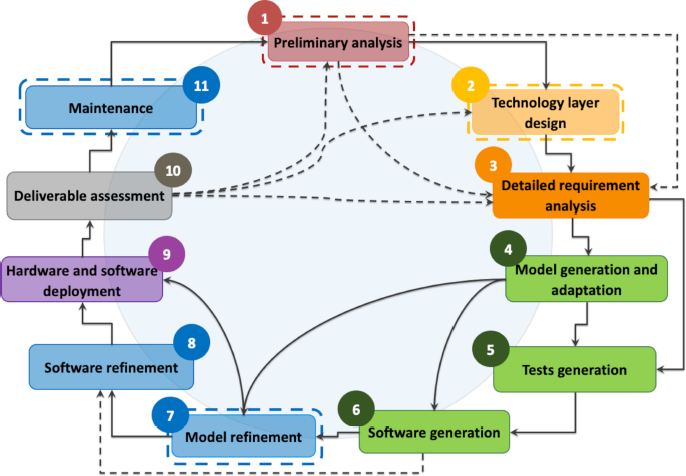
\includegraphics[width=0.8\textwidth]{images/image6.png}
				\end{figure}
				\tblnote
				
				Para FitKids, esta estructura permitió gestionar la complejidad de integrar cuatro tecnologías distintas (React Native, React, FastAPI y Gemini) de manera ordenada, con pruebas unitarias, de integración y de aceptación documentadas en las Tablas~25 a~29 del Capítulo~IV. La fase de refinamiento del modelo, propia de TDDM4IoTS y ausente en metodologías ágiles estándar, fue especialmente relevante para ajustar los diagramas UML de clases y de componentes tras la primera iteración de desarrollo, permitiendo incorporar las nuevas entidades requeridas por el módulo de supervisión parental y el sistema de recordatorios sin comprometer la consistencia arquitectónica del sistema.

		\section{Marco referencial}
			El presente marco referencial analiza investigaciones empíricas y soluciones tecnológicas publicadas en revistas indexadas JCR que abordan directamente los tres ejes técnicos de FitKids: las aplicaciones móviles de actividad física para población infantil y adolescente, los sistemas de inteligencia artificial generativa aplicados a la prescripción de ejercicio, y los modelos de aceptación tecnológica en contextos pediátricos. A diferencia del marco conceptual, que establece las bases teóricas, esta sección se enfoca en resultados empíricos y en la identificación de brechas que justifican el aporte diferenciador de FitKids.
			
			\subsection{Antecedentes de Aplicaciones Móviles de Actividad Física}
				Las soluciones tecnológicas orientadas a promover la actividad física en niños y adolescentes se han desarrollado desde cuatro enfoques complementarios: el desarrollo motor con participación familiar, la gamificación y realidad aumentada, la integración en la educación física escolar y el seguimiento de pasos. Cada línea aporta evidencia parcial sobre la efectividad de las aplicaciones móviles, pero también revela limitaciones estructurales que FitKids busca superar mediante la combinación de inteligencia artificial generativa, validación profesional y supervisión parental integrada.
			
			\subsubsection{Aplicaciones orientadas al desarrollo motor y la participación familiar}
				Zhang et al.~\cite{Zhang2024} desarrollaron y evaluaron MiniMovers, una aplicación diseñada para que los padres apoyen el desarrollo de habilidades motoras en niños de 21 a 79 meses. El estudio piloto de ocho semanas (n\,=\,8 niños con sus familias) utilizó captura de movimiento, plataforma de fuerza y rastreo ocular para medir el desempeño en seis habilidades fundamentales: correr, lanzar, saltar, patear, equilibrarse y atrapar. Los resultados evidenciaron mejoras significativas en las habilidades motoras gruesas y un incremento en la independencia de los niños durante la realización de las actividades~\cite{Zhang2024}.
				
				En una línea complementaria, Wunsch et al.~\cite{Wunsch2024} evaluaron SMARTFAMILY mediante un ensayo controlado aleatorizado por conglomerados con 46 familias. La aplicación incorporó técnicas de cambio de conducta basadas en teorías de autorregulación y establecimiento de metas, con el propósito de promover simultáneamente la actividad física y la alimentación saludable en el entorno familiar durante tres semanas de intervención activa. Sin embargo, el estudio no encontró incrementos estadísticamente significativos en actividad física ni en alimentación saludable respecto al grupo control (todos los valores p\,>\,.30), y los propios autores concluyen que la muestra estudiada ya excedía ampliamente las recomendaciones de la OMS en actividad física moderada a vigorosa, lo que limitó el margen de mejora detectable~\cite{Wunsch2024}. Tanto MiniMovers como SMARTFAMILY documentan que el padre enfrenta barreras de tiempo y orientación técnica que las aplicaciones existentes no han resuelto de forma sistemática. FitKids responde a esta limitación mediante recordatorios push configurables y un panel de estadísticas que informa al padre sin requerir su presencia constante durante la sesión de ejercicio~\cite{Zhang2024,Wunsch2024}.
			
			\subsubsection{Aplicaciones de gamificación y realidad aumentada}
				Willinger et al.~\cite{Willinger2024} evaluaron KIJANI, una aplicación que emplea gamificación y realidad aumentada para motivar a niños y adolescentes de 10 a 14 años a incrementar su actividad física diaria. Los participantes acumulaban monedas virtuales a través del movimiento físico y las usaban para construir edificios en su entorno real mediante realidad aumentada. Los resultados del estudio multimétodo mostraron evaluaciones positivas en perspicuidad (2,15 sobre 3,0 en el cuestionario UEQ) y atractividad (1,78), con adherencia sostenida durante el período de evaluación, confirmando el potencial de la gamificación para mantener el engagement en población infantil~\cite{Willinger2024}.
				
				Domin et al.~\cite{Domin2022} desarrollaron una intervención mHealth personalizada basada en teoría del comportamiento para adolescentes de 16 a 18 años, combinando una aplicación con prompts adaptativos y una pulsera Fitbit. En el estudio piloto intra-sujeto, los resultados mostraron evidencia inicial de efectividad sobre el conteo de pasos, el tiempo sedentario y los minutos de actividad física moderada a vigorosa, siendo la personalización de los prompts el factor que más contribuyó a la adherencia~\cite{Domin2022}. Sin embargo, tanto KIJANI como la intervención de Domin et al. comparten una limitación estructural: no adaptan el contenido al estado de salud individual del usuario ni cuentan con un filtro profesional previo a la entrega del ejercicio. FitKids aborda ambas brechas mediante su motor de IA generativa y su flujo obligatorio de revisión por especialistas~\cite{Zaleski2026,Dergaa2024}.
			
			\subsubsection{Aplicaciones en el contexto de la educación física escolar}
				Papastergiou et al.~\cite{Papastergiou2021} investigaron el efecto de integrar tabletas y una aplicación de fitness en clases de educación física en escuelas primarias con 145 estudiantes de 10 a 12 años distribuidos en grupos experimental y control. El grupo experimental reportó mayor interés y disfrute que el grupo control; sin embargo, no se observaron diferencias significativas en el esfuerzo percibido ni en la competencia percibida entre ambos grupos. Este hallazgo establece un límite claro: la tecnología interactiva mejora la experiencia subjetiva del ejercicio, pero no garantiza por sí sola una mayor intensidad fisiológica~\cite{Papastergiou2021}.
				
				Wang et al.~\cite{WangGamif2025} examinaron este fenómeno desde una perspectiva meta-analítica, revisando ensayos controlados aleatorizados sobre intervenciones de gamificación en niños y adolescentes publicados entre 2010 y 2024. El meta-análisis encontró efectos positivos estadísticamente significativos de la gamificación sobre la actividad física moderada a vigorosa y vigorosa, con tamaños del efecto pequeños a moderados. Crucialmente, el análisis de moderadores reveló que los efectos son sustancialmente mayores cuando la intervención incorpora metas personalizadas y retroalimentación adaptativa al nivel del usuario, frente a las que aplican los mismos elementos lúdicos de forma genérica para todos~\cite{WangGamif2025}. Este hallazgo refuerza la decisión de diseño de FitKids de combinar gamificación con personalización dinámica.
			
			\subsubsection{Intervenciones con seguimiento de pasos en adolescentes}
				Gómez-Cuesta et al.~\cite{GomezCuesta2024} realizaron un ensayo controlado aleatorizado con 462 adolescentes que usaron aplicaciones de seguimiento de pasos durante diez semanas. Los resultados mostraron mejoras en variables de grasa corporal, capacidad cardiorrespiratoria y rendimiento muscular, independientemente del estado activo o inactivo previo del participante~\cite{GomezCuesta2024}. En contraste, Mateo-Orcajada et al.~\cite{MateoOrcajada2024} evaluaron el efecto de una intervención equivalente en 50 adolescentes con sobrepeso u obesidad y no encontraron cambios estadísticamente significativos en el índice de masa corporal ni en el estado psicológico tras diez semanas.
				
				La contradicción entre ambos estudios revela que la efectividad de las aplicaciones de seguimiento de pasos depende críticamente del perfil del usuario y de la ausencia de personalización. Cuando la intervención no está calibrada a las características individuales del niño, los resultados son heterogéneos e impredecibles. La Tabla~\ref{tab:comparativa_estudios} resume los parámetros clave de los estudios revisados en esta sección.
				
				\begin{table}[H]
					\centering
					\small
					\caption[Síntesis de los estudios de aplicaciones móviles de actividad física]{Síntesis comparativa de los estudios de aplicaciones móviles de actividad física revisados}
					\label{tab:comparativa_estudios}
					\begin{tabular}{p{0.75cm}p{2.0cm}p{1.2cm}p{1.8cm}p{2.1cm}p{2.9cm}p{2.7cm}}
						\hline
						\textbf{Ref.} & \textbf{Población} & \textbf{n} & \textbf{Duración} & \textbf{Instrumento} & \textbf{Resultado principal} & \textbf{Limitación clave} \\
						\hline
						\cite{Zhang2024} & Niños 21--79 meses & 8 familias & 8 semanas & Captura de movimiento & Mejora en habilidades motoras gruesas & Muestra muy pequeña; barreras parentales de tiempo \\
						
						\cite{Wunsch2024} & Familias con hijos & 46 familias & 3 semanas (+ 4 sem. seguimiento) & Acelerometría + cuestionario & PA mantenida; sin incremento significativo (p\,>\,.30) & Muestra ya activa; sin personalización IA \\
						
						\cite{Willinger2024} & Niños 10--14 años & 22 & 10 semanas & UEQ & Perspicuidad 2,15/3,0; adherencia positiva & Sin validación clínica ni ajuste por condición médica \\
						
						\cite{Domin2022} & Adolescentes 16--18 años & Piloto & Piloto intra-sujeto & Fitbit + autoreporte & Incremento en pasos y MVPA & Sin módulo parental; solo mayores de 16 \\
						
						\cite{Papastergiou2021} & Niños 10--12 años & 145 & 1 sesión PE & Cuestionario motivación & Mayor interés y disfrute; sin cambio en esfuerzo percibido & Sin personalización; contexto escolar único \\
						
						\cite{GomezCuesta2024} & Adolescentes & 462 & 10 semanas & Acelerómetro + bioimpedancia & Mejoras en grasa corporal y condición física & Sin personalización dinámica \\
						
						\cite{MateoOrcajada2024} & Adolescentes con sobrepeso & 50 & 10 semanas & IMC + cuestionario psicológico & Sin cambios significativos en IMC ni estado emocional & Muestra clínica; sin adaptación al perfil \\
						
						\textbf{FitKids} & \textbf{Niños 6--11 años} & \textbf{15+15} & \textbf{4 semanas} & \textbf{SUS + TAM + PAQ-C} & \textbf{SUS=81,17; TAM-UP=4,37; adherencia 68\%} & \textbf{Muestra exploratoria; 4 sem. de seguimiento} \\
						\hline
					\end{tabular}
				\end{table}
				\tblnote
				
		\subsection{Ejes técnicos y estudios primarios de soporte}
			Para sustentar los pilares diferenciadores de FitKids se analizan tres ejes técnicos con base en estudios primarios de alto impacto: el uso de inteligencia artificial generativa en la prescripción de ejercicio, la efectividad de la validación profesional del contenido generado por modelos de lenguaje, y la aceptación tecnológica del sistema por parte de sus usuarios.
			
			\subsubsection{Inteligencia artificial generativa en la prescripción de ejercicio}
				Zaleski et al.~\cite{Zaleski2026} evaluaron la seguridad y viabilidad de prescripciones de ejercicio generadas por el modelo Gemini 2.5 de Google para poblaciones en riesgo clínico, utilizando tres niveles de estructuración del prompt. Los expertos evaluaron los resultados con una rúbrica estructurada que medía seguridad, viabilidad, alineación con guías clínicas y personalización. El estudio reportó alta consistencia interna en las evaluaciones de los expertos (Cronbach $\alpha > 0{,}92$), aunque el coeficiente de correlación intraclase entre evaluadores fue bajo (ICC\,(2,3)\,=\,0,139), lo que indica que la valoración del contenido generado por IA varía sustancialmente según el criterio del especialista que lo revisa. Los autores concluyen que los modelos de lenguaje de gran escala pueden servir como herramientas de apoyo a la toma de decisiones, pero que la supervisión experta es imprescindible antes de entregar cualquier prescripción al usuario~\cite{Zaleski2026}. Este hallazgo valida la arquitectura de FitKids, que utiliza precisamente el modelo Gemini y hace obligatoria la aprobación del especialista antes de publicar cualquier ejercicio.
				
				Dergaa et al.~\cite{Dergaa2024} evaluaron la prescripción de ejercicio generada por GPT-4 para cinco perfiles de pacientes con distintas condiciones de salud, encontrando que el modelo producía recomendaciones razonables en términos de modalidad e intensidad, pero tendía a omitir consideraciones de seguridad específicas para condiciones complejas como la diabetes tipo 1 o las cardiopatías congénitas. Pareek et al.~\cite{Pareek2025}, en su revisión sistemática que incluyó 10 estudios sobre IA generativa en la prescripción de ejercicio, concluyen que los modelos actuales presentan limitaciones específicas para contextos pediátricos: subestiman las restricciones de intensidad apropiadas para niños con enfermedades crónicas y tienden a proponer ejercicios diseñados para adultos con ligeras adaptaciones de nomenclatura. Ambos hallazgos fundamentan la arquitectura de doble capa de FitKids: generación mediante IA seguida de validación obligatoria por especialistas en actividad física infantil~\cite{Dergaa2024,Pareek2025}.
			
			\subsubsection[La efectividad de la validación profesional]{Efectividad de la validación profesional del contenido generado por IA}
				La literatura sobre IA en salud converge en una recomendación central: los modelos de lenguaje generativo no deben operar como sistemas autónomos de prescripción clínica, sino como asistentes bajo supervisión experta~\cite{Yim2024}. Yim et al.~\cite{Yim2024}, en su revisión narrativa sistemática publicada en \textit{JMIR Medical Informatics}, identifican que el valor clínico de la IA generativa se maximiza cuando se implementa en modo \textit{human-in-the-loop}: el modelo genera la propuesta, y el profesional la revisa, valida o rechaza antes de que llegue al paciente. La tasa de rechazo observada en FitKids durante la evaluación (16\% de los ejercicios generados) ilustra empíricamente este principio: uno de cada seis ejercicios producidos por el modelo Gemini fue rechazado por los especialistas antes de llegar al usuario, lo que demuestra que el filtro profesional cumple una función real de seguridad clínica~\cite{Yim2024,Zaleski2026}. La Figura~\ref{fig:ia_pipeline} (presentada en la subsección anterior) ilustra el flujo de generación y validación implementado en FitKids.
			
				\begin{figure}[H]
					\centering
					\caption[Flujo de generación y validación del contenido en FitKids]{Flujo de generación y validación del contenido en FitKids. La tasa de rechazo del 16\% proviene de los resultados del propio estudio (Tabla~51, Cap.~IV); la necesidad de supervisión experta es respaldada por~\cite{Yim2024,Zaleski2026}}
					\label{fig:ia_pipeline}
					\begin{tikzpicture}[
						node distance=0.6cm and 1.2cm,
						box/.style={rectangle, rounded corners=4pt, draw=black,
							fill=gray!10, text width=2.8cm, align=center,
							minimum height=1cm, font=\small},
						decision/.style={diamond, draw=black, fill=yellow!20,
							text width=2cm, align=center,
							font=\small, inner sep=2pt},
						arrow/.style={->, thick},
						redarrow/.style={->, thick, red},
						greenarrow/.style={->, thick, green!60!black}
						]
						\node[box] (padre) {Padre registra perfil del niño (5 variables)};
						\node[box, right=1.2cm of padre] (gemini) {Gemini genera rutina de ejercicios};
						\node[decision, right=1.2cm of gemini] (valid) {\mbox{¿Especialista} \mbox{aprueba?}};
						\node[box, right=1.2cm of valid] (catalogo) {Ejercicio publicado en catálogo activo};
						\node[box, below=1.2cm of valid] (ajuste) {Retroalimentación y regeneración};
						\draw[arrow] (padre) -- (gemini);
						\draw[arrow] (gemini) -- (valid);
						\draw[greenarrow] (valid) -- node[above, font=\scriptsize] {S\'{i} (84\%)} (catalogo);
						\draw[redarrow] (valid) -- node[right, font=\scriptsize] {No (16\%)} (ajuste);
						\draw[arrow] (ajuste.west) -- ++(-2.75,0) -| (gemini.south);
					\end{tikzpicture}
				\end{figure}
				\tblnote
				
			\subsubsection{Modelos de aceptación tecnológica en población pediátrica}
				El Modelo de Aceptación Tecnológica (TAM) propuesto por Davis~\cite{Davis1989} postula que la intención de uso de un sistema tecnológico está determinada principalmente por dos percepciones del usuario: la \textit{utilidad percibida} (UP) y la \textit{facilidad de uso percibida} (FU). Venkatesh et al.~\cite{Venkatesh2003} extendieron el TAM original con la \textit{Unified Theory of Acceptance and Use of Technology} (UTAUT), incorporando cuatro determinantes centrales ---expectativa de rendimiento, expectativa de esfuerzo, influencia social y condiciones facilitadoras--- con cuatro moderadores: edad, género, experiencia previa y voluntariedad de uso. El modelo UTAUT explicó entre el 69 y el 70\% de la varianza en la intención de uso en los estudios de validación originales~\cite{Venkatesh2003}.
				
				En el contexto específico de las aplicaciones de salud infantil, la evaluación de la aceptación tecnológica no puede limitarse al usuario adulto: debe considerar también la perspectiva del niño, cuya disposición a usar la aplicación está mediada por su percepción de disfrute y facilidad de interacción~\cite{Hourcade2015}. Putnam et al.~\cite{Putnam2020} documentaron que los métodos estándar de investigación de experiencia de usuario requieren adaptaciones sustanciales cuando se aplican a niños: las entrevistas estructuradas son inapropiadas para menores de 8 años, los cuestionarios Likert de 5 puntos producen respuestas sesgadas hacia los extremos, y las pruebas de usabilidad deben incorporar observación directa~\cite{Putnam2020}. Estas consideraciones justifican que FitKids haya utilizado dos instrumentos complementarios: el cuestionario SUS aplicado directamente a los niños participantes, y el cuestionario TAM para los padres o tutores, obteniendo medias de UP\,=\,4,37 y FU\,=\,4,25 (escala 1--5) en la muestra de 15 padres, ambas superiores al umbral de alta aceptación, tal como se detalla en la Sección~4.2.6 del Capítulo~IV.
			
		\subsection{Análisis Crítico Comparativo}
			El análisis conjunto de los antecedentes y los ejes técnicos permite identificar con precisión el espacio conceptual que FitKids ocupa en la literatura. Ninguno de los trabajos revisados combina simultáneamente los tres atributos que definen el aporte diferenciador del sistema: personalización dinámica mediante IA generativa calibrada al perfil individual del niño, validación profesional obligatoria del contenido antes de su entrega al usuario, y módulo estructural de supervisión parental con retroalimentación activa. La Tabla~\ref{tab:comparativa_apps} sintetiza esta comparación.
			
			\begin{table}[H]
				\centering
				\small
				\caption[Comparación de características entre aplicaciones de actividad física]{Comparación de características entre aplicaciones de actividad física infantil y FitKids~\cite{Zhang2024,Wunsch2024,Willinger2024,Domin2022,Papastergiou2021,GomezCuesta2024,MateoOrcajada2024,Zaleski2026}}
				\label{tab:comparativa_apps}
				\begin{tabular}{p{2.9cm}p{1.2cm}p{1.5cm}p{1.5cm}p{1.5cm}p{1.2cm}p{1.5cm}p{1.9cm}}
					\hline
					\textbf{Característica} & \textbf{Mini\-Movers} & \textbf{SMART\-FAMILY} & \textbf{KIJANI} & \textbf{Domin et al.} & \textbf{Sworkit Kids} & \textbf{Step-trackers} & \textbf{FitKids} \\
					\hline
					Personalización dinámica (IA) & No & No & No & Parcial & No & No & \textbf{Sí} \\
					
					Validación por especialista & Sí (diseño) & No & No & No & No & No & \textbf{Sí (pre-entrega)} \\
					
					Supervisión parental integrada & Alto & Alto & Bajo & Bajo & Bajo & Bajo & \textbf{Alto} \\
					
					Gamificación & No & Parcial & Sí & No & Sí & No & \textbf{Sí} \\
					
					Validación clínica del contenido & No & No & No & No & No & No & \textbf{Sí} \\
					
					Población objetivo & 0--6 años & Familias & 10--14 años & 16--18 años & 5--12 años & 13--18 años & \textbf{6--11 años} \\
					
					Instrumento de evaluación & Motor & Acelerómetro & UEQ & Fitbit & Cuestionario & Acelerómetro & \textbf{SUS + TAM} \\
					\hline
				\end{tabular}
			\end{table}
			\tblnote
			
			Mediante el análisis de la literatura se identificaron tres tendencias que delimitan el estado del arte. En primer lugar, las aplicaciones móviles infantiles publicadas operan mayoritariamente con catálogos predefinidos de ejercicios, lo que impide la adaptación dinámica al perfil individual del niño~\cite{Zhang2024,Papastergiou2021,Willinger2024,Wunsch2024}. En segundo lugar, los estudios que evalúan la IA generativa en la prescripción de ejercicio se han desarrollado fundamentalmente sobre población adulta y en contextos clínicos controlados~\cite{Zaleski2026,Dergaa2024,Pareek2025}. La brecha en población infantil es doble: metodológica, porque los perfiles de niños de 6 a 11 años requieren umbrales de seguridad distintos; y técnica, porque los prompts diseñados para adultos no incorporan las restricciones apropiadas para el desarrollo motor en edad escolar. En tercer lugar, la participación parental se identifica en todos los trabajos como factor determinante de la adherencia, pero en la mayoría de los sistemas existentes el padre opera como observador pasivo sin herramientas de seguimiento estructuradas~\cite{Zhang2024,GomezCuesta2024,MateoOrcajada2024}.
			
			La Figura~\ref{fig:radar_comparativo} ilustra visualmente la posición de FitKids frente a las soluciones revisadas en cinco dimensiones clave.
			
			\begin{figure}[H]
				\centering
				\caption[Comparación en dimensiones de diseño entre FitKids y otras soluciones]{Comparación en cinco dimensiones de diseño (escala 1--5) entre FitKids y soluciones de la literatura~\cite{Willinger2024,Wunsch2024,GomezCuesta2024,MateoOrcajada2024}}
				\label{fig:radar_comparativo}
				\begin{tikzpicture}
					\begin{polaraxis}[
						xtick={0,72,144,216,288},
						xticklabels={Personalización IA, Validación clínica, Supervisión parental, Gamificación, Evaluación UX},
						xticklabel style={font=\scriptsize},
						ymin=0, ymax=5,
						ytick={1,2,3,4,5},
						yticklabel style={font=\tiny},
						grid=both,
						width=9cm,
						legend style={at={(1.35,1)}, anchor=north, font=\scriptsize}
						]
						\addplot[thick, blue, fill=blue!20, opacity=0.5] coordinates {
							(0,5)(72,5)(144,5)(216,5)(288,5)(360,5)
						};
						\addlegendentry{FitKids}
						\addplot[thick, red, fill=red!20, opacity=0.4] coordinates {
							(0,1)(72,1)(144,2)(216,5)(288,2)(360,1)
						};
						\addlegendentry{KIJANI}
						\addplot[thick, green!60!black, fill=green!20, opacity=0.4] coordinates {
							(0,1)(72,1)(144,4)(216,3)(288,2)(360,1)
						};
						\addlegendentry{SMARTFAMILY}
						\addplot[thick, orange, fill=orange!20, opacity=0.4] coordinates {
							(0,2)(72,1)(144,1)(216,1)(288,2)(360,2)
						};
						\addlegendentry{Step-trackers}
					\end{polaraxis}
				\end{tikzpicture}
			\end{figure}
			\tblnote
			
			FitKids invierte la lógica pasiva del padre al posicionarlo como actor activo del sistema, con acceso a estadísticas de progreso, notificaciones push configurables y capacidad de ajuste del perfil del niño en tiempo real, en línea con la evidencia sobre el correlato parental como el predictor más consistente de la actividad física infantil~\cite{Yao2015,VegaDiaz2023}. La combinación de estos tres atributos ausentes en la literatura define el espacio de innovación que FitKids ocupa y justifica su evaluación empírica en el contexto ecuatoriano con población de 6 a 11 años.

	\capituloseparador{III}{METODOLOGÍA}
	\label{ch:metodologia}
		\section{Localización}
			El proyecto se desarrolló en la Universidad Técnica Estatal de Quevedo (UTEQ), en el campus ``Central'', ubicado en la Av. Quito km. 11/2 vía a Santo Domingo de los Tsáchilas, en el cantón de Quevedo, provincia de Los ríos, Ecuador.
		
			\begin{figure}[H]
				\centering
				\caption{Localización de la Universidad Técnica Estatal de Quevedo}
				\label{fig:loc}
				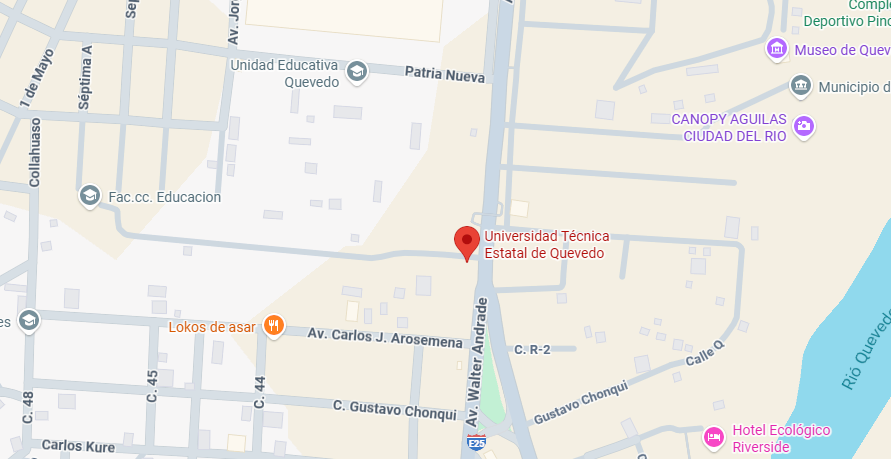
\includegraphics[width=0.9\textwidth]{images/image8.png}
			\end{figure}
			\tblnote
		
		\section{Tipo de investigación}
			Para este proyecto se utilizó dos tipos de investigación: la aplicada y la descriptiva.
		
			\subsection{Aplicada}
				La investigación aplicada busca utilizar el conocimiento científico existente para resolver problemas concretos o mejorar situaciones específicas del entorno real~\cite{HernandezSampieri2014}. Bajo este enfoque, el presente proyecto implicó el desarrollo de FitKids, una aplicación móvil que utiliza inteligencia artificial generativa para crear planes de ejercicio físico personalizados para niños de 6 a 11 años. La aplicación tiene como objetivo fomentar hábitos saludables y mejorar el bienestar físico y emocional mediante rutinas adaptadas a las necesidades, preferencias y condición de salud de cada niño, promoviendo así su participación activa y sostenida~\cite{Direito2017,WangGamif2025}.
				Esta solución responde a una problemática documentada: el sedentarismo infantil afecta a más del 81,\% de los adolescentes a nivel mundial~\cite{Guthold2020}, con consecuencias negativas en el desarrollo físico, emocional y social de los niños~\cite{Musa2022,Wilhite2023}. Al promover un estilo de vida activo a través de rutinas generadas por IA y validadas por especialistas, FitKids contribuye al desarrollo integral del niño: la actividad física regular produce beneficios documentados como mayor capacidad cardiovascular, mejor concentración, reducción de la ansiedad y un estado de ánimo más positivo~\cite{Li2022,Bull2020}.
			
			\subsection{Descriptiva}
				La investigación descriptiva busca especificar las propiedades, características y perfiles de fenómenos sometidos a análisis, midiendo o recopilando información sobre las variables de estudio de forma independiente con el fin de describir con precisión lo que se investiga~\cite{HernandezSampieri2014}. Bajo este alcance, el presente proyecto ofreció un panorama detallado sobre la construcción de FitKids como herramienta tecnológica: se caracterizaron los requisitos funcionales y no funcionales del sistema, se describió el proceso de integración del motor de inteligencia artificial generativa para la personalización de rutinas de ejercicio, y se documentaron las funcionalidades implementadas para el monitoreo parental y la validación clínica del contenido~\cite{GuerreroUlloa2024}.
				
				El enfoque descriptivo permitió además caracterizar a la población participante ---15 niños de 6 a 11 años y 15 padres o tutores--- y describir los resultados obtenidos en los instrumentos de evaluación aplicados: el cuestionario SUS para medir la usabilidad del sistema y el cuestionario TAM para evaluar la aceptación tecnológica por parte de los padres. Este tipo de investigación no establece relaciones causales entre variables, sino que documenta con precisión el comportamiento del sistema y las percepciones de los usuarios en un contexto real de uso~\cite{HernandezSampieri2014}.
		
		\section{Método de investigación}
			Para el desarrollo del sistema FitKids se aplicó un enfoque metodológico mixto que integra el razonamiento deductivo e inductivo, permitiendo una transición lógica entre el levantamiento de necesidades específicas del contexto y la implementación técnica de la solución~\cite{Creswell2018}.
			
			\subsection{Método Deductivo}
				La investigación deductiva parte de principios generales o teorías previamente establecidas para llegar a conclusiones específicas aplicables a un problema concreto. Se basa en la lógica formal y permite validar soluciones mediante la aplicación de modelos preexistentes, generando conocimiento con certeza y consistencia sin depender del número de casos observados~\cite{HernandezSampieri2014}.
				
				En el presente proyecto, el método deductivo orientó el diseño de FitKids a partir de teorías generales sobre sedentarismo infantil, personalización de intervenciones mediante inteligencia artificial y modelos de aceptación tecnológica~\cite{Davis1989,WangGamif2025}. Partiendo de estos marcos teóricos consolidados, se derivaron los requisitos funcionales del sistema, se definieron los criterios de diseño de la interfaz infantil y se establecieron los umbrales de evaluación de usabilidad y aceptación empleados en la fase de validación~\cite{HernandezSampieri2014,Bull2020}.
				
			\subsection{Método Inductivo}
				Creswell y Creswell~\cite{Creswell2018} explica que la inducción es un proceso mental que parte de la observación de casos particulares para llegar a conclusiones o leyes generales aplicables a fenómenos más amplios. A través de este razonamiento, el investigador acumula evidencia empírica específica y la sintetiza en principios que orientan el diseño de soluciones~\cite{Creswell2018}.
				
				Mediante las entrevistas semiestructuradas realizadas a especialistas en actividad física infantil y a padres de familia, se recolectaron observaciones específicas sobre las barreras del sedentarismo en niños de 6 a 11 años y sobre las preferencias de uso tecnológico en el contexto de Quevedo. A partir de estos datos particulares se indujeron los requisitos generales y las funcionalidades necesarias del sistema: la personalización de rutinas mediante IA generativa, el módulo de supervisión parental y el flujo de validación profesional del contenido, garantizando que la solución respondiera a necesidades reales documentadas en campo~\cite{Creswell2018,Direito2017}.
		
		
		\section{Técnicas de investigación}
			En el presente proyecto se emplearon dos técnicas de investigación complementarias: la revisión de la literatura y la entrevista semiestructurada. La primera permitió construir el marco teórico y definir los ejes temáticos del estudio; la segunda posibilitó recopilar información contextualizada directamente desde los actores del problema~\cite{HernandezSampieri2014,Creswell2018}.
			
			\subsection{Revisión de la literatura}
				La revisión de la literatura es un proceso sistemático de búsqueda, análisis y síntesis de información relevante y actualizada sobre un tema específico, extraída de fuentes confiables como artículos científicos, libros académicos y estudios previos~\cite{HernandezSampieri2014}. En este proyecto se llevó a cabo una revisión orientada a identificar el estado del arte sobre sedentarismo infantil, recomendaciones internacionales de actividad física, aplicaciones mHealth para niños e inteligencia artificial generativa aplicada a la prescripción de ejercicio~\cite{Guthold2020,Bull2020,Direito2017}.
				
				Esta revisión cumplió una doble función metodológica. Por un lado, fundamentó el marco teórico y referencial del proyecto con evidencia científica de alto impacto~\cite{WangGamif2025,Schoeppe2017}. Por otro lado, orientó el diseño de las entrevistas semiestructuradas: a partir de los temas identificados en la literatura ---necesidades físicas, emocionales y sociales de los niños, criterios de personalización del ejercicio y estrategias de adherencia--- se derivaron los ejes de indagación del guion de entrevista, garantizando que las preguntas fueran pertinentes y fundamentadas en evidencia~\cite{Creswell2018,HernandezSampieri2014}.
			
			\subsection{Entrevista}
				La entrevista semiestructurada es una técnica de recolección de datos que combina preguntas predefinidas con la flexibilidad de explorar respuestas emergentes, permitiendo al investigador profundizar en opiniones, experiencias y conocimientos prácticos de los participantes sobre el fenómeno estudiado~\cite{Creswell2018}. Su uso está ampliamente respaldado en investigación aplicada al diseño de sistemas de salud digital, donde el levantamiento de requisitos depende del conocimiento experto y del contexto real de los usuarios~\cite{HernandezSampieri2014}.
				
				Se realizaron siete entrevistas semiestructuradas: cuatro dirigidas a especialistas en actividad física infantil y pediatría, y tres a padres de familia de niños de 6 a 11 años residentes en Quevedo. Las preguntas abiertas se organizaron en torno a tres ejes temáticos: (1) tipos de ejercicio más adecuados según la edad y condición del niño; (2) frecuencia, duración e intensidad recomendadas conforme a las guías de la OMS~\cite{Bull2020}; y (3) estrategias y elementos que favorecen la adherencia sostenida a la actividad física en la infancia~\cite{Yao2015,VegaDiaz2023}. La información obtenida permitió derivar inductivamente los requisitos funcionales y no funcionales del sistema FitKids, asegurando que la solución tecnológica respondiera a necesidades reales documentadas en campo~\cite{Creswell2018}.
		
		\section{Recursos, presupuesto y financiamiento}
			En este apartado se describen los recursos utilizados para el desarrollo del sistema FitKids, así como el presupuesto estimado y las fuentes de financiamiento empleadas. La identificación y planificación de estos elementos permitió garantizar la viabilidad del proyecto y el adecuado desarrollo de las actividades previstas, considerando los recursos humanos, técnicos y materiales necesarios para la implementación del sistema.
			
			\subsection{Equipo de trabajo}
				El desarrollo de FitKids contó con la participación de un equipo de trabajo conformado por la autora del proyecto, el director del proyecto y el tutor académico. Cada uno desempeñó un rol específico que contribuyó al cumplimiento de los objetivos establecidos y al correcto desarrollo del sistema.
				
				La autora del proyecto asumió el rol de equipo de desarrollo, siendo responsable del análisis, diseño, implementación y documentación del sistema. El director del proyecto actuó como facilitador del proceso, brindando orientación técnica y metodológica durante las distintas etapas del proyecto conforme a la metodología TDDM4IoTS~\cite{GuerreroUlloa2024}. Por su parte, el tutor académico proporcionó acompañamiento y asesoría académica, asegurando que el proyecto cumpliera con los lineamientos institucionales y los estándares establecidos para el trabajo de titulación.
				
				\begin{table}[H]
					\centering
					\small
					\caption{Equipo de trabajo y roles en el proyecto}
					\label{tab:equipo}
					\begin{tabular}{p{4.7cm}p{4.7cm}p{4.7cm}}
						\hline
						\textbf{Integrante} & \textbf{Correo institucional} & \textbf{Rol} \\
						\hline
						PhD. Gleiston Guerrero Ulloa & gguerrero@uteq.edu.ec & Facilitador del proyecto \\
						
						Valeska Sofia Chica Valfre & vchicav@uteq.edu.ec & Equipo de desarrollo \\
						\hline
					\end{tabular}
				\end{table}
				\tblnote
			
			\subsection{Tecnologías y herramientas utilizadas}
				La selección de las tecnologías y herramientas para el desarrollo del sistema FitKids estuvo guiada por cuatro criterios transversales aplicados a cada componente de la arquitectura: \textbf{compatibilidad entre capas}, para garantizar que las tecnologías de presentación, servicios, negocio y datos pudieran integrarse sin capas de adaptación que incrementaran la complejidad del sistema~\cite{Kleppmann2017}; \textbf{madurez y soporte activo de la comunidad}, con preferencia por tecnologías ampliamente adoptadas y documentadas que redujeran el riesgo de bloqueo técnico durante el desarrollo~\cite{Fowler2002}; \textbf{adecuación al contexto del proyecto}, considerando que se trata de un prototipo académico con recursos humanos y económicos limitados, lo que favoreció soluciones con capas gratuitas funcionales y curvas de aprendizaje razonables; y \textbf{coherencia con los requerimientos no funcionales del sistema}, particularmente los atributos de seguridad, mantenibilidad y eficiencia de desempeño establecidos conforme a la norma ISO/IEC~25010~\cite{ISO25010,GuerreroUlloa2024}. Las tablas que siguen registran las tecnologías y herramientas seleccionadas a partir de ese proceso, organizadas en tres grupos que distinguen entre componentes del producto, herramientas del proceso de desarrollo y herramientas de soporte a la gestión.
				
				La Tabla~\ref{tab:tecnologias} presenta las tecnologías que conforman el sistema FitKids, organizadas por capa arquitectónica.
				
				\begingroup
				\setlength{\LTpre}{6pt}\setlength{\LTpost}{2pt}
				\renewcommand{\arraystretch}{1.15}
				\small
				\begin{longtable}{p{2.8cm}p{3.3cm}p{3.5cm}p{4.4cm}}
					\caption{Tecnologías de desarrollo}\label{tab:tecnologias}\\
					\hline
					\textbf{Categoría} & \textbf{Tecnología} & \textbf{Descripción} & \textbf{Uso en el proyecto}\\
					\hline
					\endfirsthead
					
					\textbf{Categoría} & \textbf{Tecnología} & \textbf{Descripción} & \textbf{Uso en el proyecto}\\
					
					\endhead
					\multicolumn{4}{r}{\footnotesize\itshape continúa $\rightarrow$}\\
					\endfoot
					
					\endlastfoot
					Frontend móvil & React Native 0.81.4 & Framework para desarrollo de aplicaciones móviles multiplataforma & Desarrollo del entorno orientado a niños y padres: visualización de rutinas, seguimiento del progreso y gestión de recordatorios\\
					Entorno móvil & Expo \textasciitilde{}54.0.13 & Plataforma que facilita el desarrollo, prueba y ejecución de aplicaciones móviles & Simplificación del desarrollo y despliegue del entorno móvil\\
					Lenguaje frontend móvil & TypeScript & Lenguaje que extiende JavaScript con tipado estático & Desarrollo del frontend móvil, mejorando la mantenibilidad y control del código\\
					Frontend web & React \^{}19.2.0 & Biblioteca JavaScript para la creación de interfaces de usuario & Desarrollo del entorno web destinado a especialistas para la revisión y validación de ejercicios\\
					Lenguaje frontend web & JavaScript & Lenguaje de programación interpretado para aplicaciones web & Creación de interfaces dinámicas en el frontend web\\
					Backend & FastAPI $\geq$0.100.0 & Framework para el desarrollo de servicios web y APIs REST & Gestión de la lógica del sistema y el procesamiento de solicitudes\\
					Lenguaje backend & Python $\geq$3.10 & Lenguaje de programación de alto nivel & Implementación de la lógica del servidor e integración con la inteligencia artificial\\
					Base de datos & PostgreSQL 17.8 & Sistema gestor de bases de datos relacional & Almacenamiento de datos de usuarios, rutinas y registros de actividad física\\
					Inteligencia artificial & Gemini API $\geq$0.2.0 & Modelo de inteligencia artificial generativa de Google & Generación de planes de ejercicios personalizados e imágenes ilustrativas\\
					Notificaciones & OneSignal $\geq$0.2.0 & Servicio de notificaciones push & Envío de recordatorios de actividad física a padres y niños\\
				\end{longtable}
				\vspace{12pt}
				\tblnote
				\endgroup
				
				La coherencia interna de la pila tecnológica adoptada —React Native y React como base común de los dos frontends, Python como lenguaje unificado del backend y de la integración con IA, y PostgreSQL como repositorio relacional con garantías de integridad— reduce la fragmentación cognitiva del equipo de desarrollo y facilita el mantenimiento futuro del sistema, atributo directamente relacionado con la dimensión de mantenibilidad del modelo ISO/IEC~25010~\cite{ISO25010,Fowler2002,GuerreroUlloa2024}.
				
				\begin{table}[H]
					\centering
					\small
					\caption{Herramientas de desarrollo}
					\label{tab:herramientas}
					\begin{tabular}{p{2.2cm}p{5.1cm}p{7.1cm}}
						\hline
						\textbf{Software} & \textbf{Descripción} & \textbf{Uso} \\
						\hline
						Visual Studio Code & Editor de código multiplataforma con compatibilidad con diversos lenguajes y extensiones & Entorno de desarrollo principal para la programación del frontend (React Native, React) y el backend (FastAPI) \\
						
						DBeaver & Herramienta de administración de bases de datos con interfaz gráfica & Administración y gestión de la base de datos: consultas, verificación de tablas y control de la estructura de la información \\
						
						GitHub & Plataforma de control de versiones y trabajo colaborativo & Gestión de versiones del proyecto y apoyo a los procesos de integración continua \\
						
						Postman & Herramienta para el diseño, prueba y verificación de APIs & Verificación del correcto funcionamiento de los servicios del backend y validación de la comunicación entre componentes \\
						
						Render & Servicio de despliegue y alojamiento de aplicaciones & Hospedaje del backend del sistema, garantizando la disponibilidad del servicio y el acceso remoto \\
						
						Neon & Plataforma en la nube para bases de datos PostgreSQL administradas & Alojamiento de la base de datos en entorno de producción, garantizando rendimiento, disponibilidad y seguridad \\
						\hline
					\end{tabular}
				\end{table}
				\tblnote
				
				La Tabla~\ref{tab:herramientas} describe las herramientas que estructuraron el proceso de desarrollo, testing y despliegue del sistema.
				
				Las herramientas del proceso de desarrollo se seleccionaron para materializar un flujo de trabajo con puntos de verificación explícitos: el control de versiones en GitHub garantiza la trazabilidad de cada cambio; Postman permite validar los contratos de la API de forma independiente antes de la integración con los clientes; y el par Render--Neon traslada el sistema a un entorno de producción real sin incurrir en costos que excedan el presupuesto académico disponible~\cite{GuerreroUlloa2024,Fowler2002}.
				
				
				La Tabla~\ref{tab:complementarias} recoge las herramientas de soporte utilizadas para la gestión, documentación y comunicación del proyecto.
				
				\begin{table}[H]
					\centering
					\small
					\caption{Herramientas complementarias}
					\label{tab:complementarias}
					\begin{tabular}{p{2.5cm}p{4.9cm}p{7.0cm}}
						\hline
						\textbf{Software} & \textbf{Descripción} & \textbf{Uso} \\
						\hline
						Windows 11 & Sistema operativo instalado en los equipos del equipo de trabajo & Ejecución de las herramientas de desarrollo y administración general del proyecto \\
						
						Microsoft Word & Procesador de texto para la creación y edición de documentos & Elaboración de informes técnicos y redacción del documento de tesis \\
						
						Microsoft Excel & Aplicación de hoja de cálculo para el manejo y análisis de datos & Organización, procesamiento y análisis de la información recopilada durante el proyecto \\
						
						Canva & Herramienta para la creación de presentaciones digitales & Preparación de exposiciones del proyecto para la presentación de avances y resultados \\
						\hline
					\end{tabular}
				\end{table}
				\tblnote
				
				La distinción entre componentes del producto, herramientas del proceso y herramientas de soporte no es meramente organizativa: responde al principio de separación entre decisiones técnicas de construcción ---que impactan directamente sobre los atributos de calidad del sistema--- y decisiones operativas de gestión, cuyo efecto recae sobre la eficiencia del proceso de desarrollo~\cite{Fowler2002}. Esta distinción facilita la evaluación independiente de ambas dimensiones durante las fases de verificación y validación del proyecto.
				
			\subsection{Estimación de costos}
				El presupuesto del proyecto se estructuró en dos categorías: equipamiento físico, conformado por los dispositivos requeridos para el desarrollo y la ejecución de pruebas del sistema, y servicios en la nube, correspondientes a las plataformas de despliegue y gestión de base de datos empleadas durante el período de desarrollo activo. En proyectos de software de alcance académico, la estimación de costos suele restringirse a los recursos directamente vinculados al ciclo de vida del producto, excluyendo gastos operativos indirectos que no afectan el desarrollo del artefacto tecnológico~\cite{Pressman2019}; bajo este criterio, la estimación de FitKids consideró únicamente los insumos tecnológicos imprescindibles para la construcción y funcionamiento del sistema.
				
				La adopción de plataformas en la nube con esquemas de pago por uso, como Render para el despliegue del backend y Neon para la gestión serverless de la base de datos PostgreSQL, respondió a una decisión deliberada de minimizar los costos de infraestructura sin comprometer la disponibilidad del servicio durante el período de evaluación. Wen et al.~\cite{Wen2023} documentan que el modelo serverless libera al equipo de desarrollo de la administración de servidores y reduce significativamente los costos operativos en comparación con el despliegue en infraestructura convencional, lo que lo convierte en una opción particularmente adecuada para prototipos con recursos limitados. El detalle de cada concepto y su valoración se presenta en la Tabla~\ref{tab:costos}.
				
				\begin{table}[H]
					\centering\small
					\caption{Estimación de costos del proyecto}
					\label{tab:costos}
					\begin{tabular}{p{5.1cm}>{\centering\arraybackslash}p{2.2cm}>{\raggedleft\arraybackslash}p{3.5cm}>{\raggedleft\arraybackslash}p{2.7cm}}
						\hline
						\textbf{Concepto} & \textbf{Cantidad} & \textbf{Costo unitario (USD)} & \textbf{Subtotal (USD)}\\
						\hline
						Laptop HP & 1 & 450{,}00 & 450{,}00\\
						Dispositivos móviles Android & 2 & 100{,}00 & 200{,}00\\
						Servicio Render (mensual) & 6 & 7{,}00 & 42{,}00\\
						Servicio Neon (mensual) & 6 & 10{,}00 & 60{,}00\\
						Horas de desarrollo (estimado) & 700 & 1{,}00 & 700{,}00\\
						\textbf{Total} & & & \textbf{1\,452{,}00}\\
						\hline
					\end{tabular}
				\end{table}
				\tblnote
				
			\subsection{Consideraciones éticas y de privacidad}
				El desarrollo del sistema FitKids implicó el tratamiento de datos personales de menores de edad, lo que exige un nivel de protección superior al requerido para usuarios adultos. A continuación se detallan las medidas adoptadas en materia de privacidad, consentimiento y uso responsable de la inteligencia artificial generativa.
				
				\subsubsection{Consentimiento informado y base legal}
					La participación de los niños en la evaluación del sistema requirió la autorización expresa de sus representantes legales, documentada mediante formularios de consentimiento informado (Anexo~5). Este procedimiento se enmarca en el artículo 24 de la Ley Orgánica de Protección de Datos Personales del Ecuador~\cite{LOPDP2021}, que establece que los niños, niñas y adolescentes menores de 15 años necesitarán de su representante legal para el ejercicio de sus derechos en materia de datos personales. El procedimiento se alinea además con el principio de transparencia reconocido por el Reglamento General de Protección de Datos de la Unión Europea~\cite{GDPR2016}, adoptado como estándar internacional de referencia en materia de privacidad de datos de menores.
					
				\subsubsection{Datos recopilados y nivel de sensibilidad}
					La Tabla~\ref{tab:datos_privacidad} detalla los datos que el sistema recopila, su naturaleza, la forma de almacenamiento y quién puede acceder a ellos. El procesamiento local de imágenes de movimiento ---mediante comparación de fotogramas en formato base64 directamente en el dispositivo--- constituye la medida de privacidad técnica más relevante del sistema: impide la transmisión de datos biométricos hacia servidores externos, en línea con el principio de minimización de datos establecido en el artículo 5.1(c) del RGPD~\cite{GDPR2016} y recogido en la LOPDP ecuatoriana~\cite{LOPDP2021}.
					
					\begin{table}[H]
						\centering
						\small
						\caption{Datos personales recopilados por FitKids: sensibilidad y tratamiento}
						\label{tab:datos_privacidad}
						\begin{tabular}{p{2.0cm}p{2.0cm}p{2.8cm}p{2.8cm}p{3.4cm}}
							\hline
							\textbf{Dato} & \textbf{Sensibilidad} & \textbf{Almacenamiento} & \textbf{Acceso} & \textbf{Periodo de retención} \\
							\hline
							Apodo del niño & Baja & BD cifrada en Neon & Padre autenticado & Duración de la cuenta \\
							
							Fecha de nacimiento & Media & BD cifrada en Neon & Padre autenticado & Duración de la cuenta \\
							
							Peso y talla & Media & BD cifrada en Neon & Padre autenticado & Duración de la cuenta \\
							
							Condiciones médicas & Alta & BD cifrada en Neon & Padre y especialista autenticados & Duración de la cuenta \\
							
							Intereses deportivos & Baja & BD cifrada en Neon & Padre autenticado y sistema de IA & Duración de la cuenta \\
							
							Tiempo de ejercicio & Baja & BD cifrada en Neon & Padre autenticado & 12 meses \\
							
							Imágenes de movimiento & Alta --- dato biométrico & Procesamiento local en el dispositivo; no se almacenan & Ningún actor del sistema & No se retienen \\
							\hline
						\end{tabular}
					\end{table}
					\tblnote
					
				\subsubsection{Límites del sistema de IA y salvaguardas}
					El modelo Gemini, utilizado para la generación de rutinas e imágenes ilustrativas, puede producir contenido que, aun siendo lingüísticamente correcto, resulte clínicamente inadecuado para la población infantil. La tasa de rechazo observada durante la evaluación (16\% de los ejercicios generados) evidencia empíricamente esta limitación, coherente con los hallazgos de Zaleski et al.~\cite{Zaleski2026} y Dergaa et al.~\cite{Dergaa2024} sobre las restricciones de los modelos de lenguaje en contextos de prescripción de actividad física. Para mitigar este riesgo, el sistema implementa dos salvaguardas complementarias: (1)~restricciones programadas en el prompt de generación, que definen explícitamente los límites de intensidad, duración y tipo de ejercicio según el rango de edad y las condiciones médicas declaradas; y (2)~un filtro humano obligatorio operado por especialistas en actividad física infantil, quienes revisan y aprueban cada ejercicio antes de su publicación en el catálogo activo, conforme al modelo \textit{human-in-the-loop} recomendado para sistemas de IA en salud~\cite{Yim2024}. Ningún contenido generado por IA llega al usuario final sin haber superado ambas salvaguardas.
					
		\section{Instrumentos para el seguimiento y control}
			El seguimiento y control del proyecto tecnológico FitKids constituyó un proceso fundamental para garantizar el cumplimiento de los objetivos establecidos, el control de los tiempos de ejecución y la calidad del producto desarrollado~\cite{Fowler2002}. Se emplearon instrumentos que permitieron monitorear el avance del proyecto, coordinar actividades, gestionar la documentación y controlar las versiones del software durante todas las fases de desarrollo, en correspondencia con las prácticas estándar de gestión de proyectos tecnológicos~\cite{GuerreroUlloa2024}.
				
			\subsection{Herramientas de gestión del proyecto}
				Para la planificación y control del avance del proyecto se utilizó el diagrama de Gantt, el cual permitió organizar y visualizar las actividades desarrolladas a lo largo de los semestres noveno y décimo~\cite{Creswell2018}. Este instrumento facilitó el seguimiento de los plazos, la identificación de dependencias entre tareas y el control del cumplimiento de los hitos establecidos.
				
				La comparación entre la planificación inicial y la ejecución real permitió detectar oportunamente posibles retrasos y aplicar acciones correctivas cuando fue necesario, garantizando la alineación del desarrollo con los objetivos y el cronograma establecidos~\cite{Fowler2002}.
				
			\subsection{Herramientas de comunicación}
				La comunicación entre la autora del proyecto y el director se realizó mediante Google Meet, plataforma que permitió llevar a cabo reuniones virtuales de seguimiento, revisión de avances y retroalimentación técnica y metodológica~\cite{GuerreroUlloa2024}. La periodicidad de estas reuniones aseguró la coordinación oportuna durante todas las etapas del desarrollo.
				
				El intercambio de observaciones y la toma de decisiones a través de esta herramienta contribuyeron a mantener la coherencia entre los objetivos del proyecto y las decisiones de implementación adoptadas en cada fase, reduciendo los tiempos de resolución de incidencias técnicas y académicas~\cite{Fowler2002,GuerreroUlloa2024}.
				
				La Tabla~\ref{tab:reuniones} sintetiza la frecuencia y propósito de las reuniones de seguimiento realizadas durante el desarrollo del proyecto.
				
				\begin{table}[H]
					\centering
					\small
					\caption{Reuniones de seguimiento realizadas durante el desarrollo de FitKids}
					\label{tab:reuniones}
					\begin{tabular}{p{4.1cm}p{2.5cm}p{7.2cm}}
						\hline
						\textbf{Etapa} & \textbf{Frecuencia} & \textbf{Propósito principal} \\
						\hline
						Titulación I & Quincenal & Definición de objetivos, revisión del marco teórico y diseño del sistema \\
						
						Titulación II (desarrollo) & Semanal & Revisión de avances de implementación y resolución de incidencias técnicas \\
						
						Titulación II (evaluación) & Semanal & Revisión de resultados, análisis de datos y ajustes al documento final \\
						\hline
					\end{tabular}
				\end{table}
				\tblnote
				
			\subsection{Herramientas de gestión de documentos}
				Para la organización, almacenamiento y respaldo de la documentación del proyecto se emplearon las plataformas Google Drive y OneDrive~\cite{Kleppmann2017}. Estas herramientas permitieron gestionar de manera ordenada los documentos académicos, archivos técnicos, diagramas y evidencias del desarrollo, garantizando el acceso remoto y la preservación de versiones actualizadas.
				
				La disponibilidad permanente de la documentación en la nube facilitó la revisión colaborativa entre la autora y el director del proyecto, reduciendo los riesgos de pérdida de información y asegurando la trazabilidad de los cambios realizados a lo largo del ciclo de vida del proyecto~\cite{Fowler2002}.
				
				La Tabla~\ref{tab:documentos} resume los tipos de documentos gestionados y las plataformas utilizadas para su almacenamiento.
				
				\begin{table}[H]
					\centering
					\small
					\caption{Tipos de documentos gestionados y plataformas de almacenamiento}
					\label{tab:documentos}
					\begin{tabular}{p{5cm}p{3.5cm}p{5.5cm}}
						\hline
						\textbf{Tipo de documento} & \textbf{Plataforma} & \textbf{Descripción} \\
						\hline
						Documento de tesis & GitHub & Versiones del documento LaTeX, Bibliografía e imágenes\\
						
						Diagramas y modelos del sistema & Google Drive/GitHub & Diagramas UML, arquitectura y flujos del sistema \\
						
						Instrumentos de evaluación & Google Drive & Formularios SUS, TAM y consentimientos informados \\
						
						Evidencias de reuniones & Google Drive & Capturas, actas y grabaciones de sesiones de seguimiento \\
						\hline
					\end{tabular}
				\end{table}
				\tblnote
				
			\subsection{Control de versiones del software}
				El control de versiones del software desarrollado se realizó mediante Git, utilizando la plataforma GitHub como repositorio remoto~\cite{Kleppmann2017}. Estas herramientas permitieron registrar los cambios realizados en el código fuente, mantener un historial de modificaciones y facilitar la recuperación de versiones anteriores en todos los componentes del sistema: backend (FastAPI/Python), frontend móvil (React Native/TypeScript) y frontend web (React/JavaScript). El flujo de trabajo adoptado organizó el desarrollo en una rama principal (\texttt{main}) protegida para las versiones estables y ramas de funcionalidad (\texttt{feature/*}) para el desarrollo incremental de cada módulo, fusionadas mediante \textit{pull requests} revisados antes de su integración, conforme a las prácticas estándar de ingeniería de software colaborativo~\cite{Fowler2002,Kleppmann2017}.
				
				Las pruebas unitarias y de integración descritas en las secciones~3.7 y~4.1 se ejecutaron de forma automatizada mediante Pytest en el backend y mediante Jest y Vitest en los frontends, en línea con el principio de desarrollo guiado por pruebas que establece la metodología TDDM4IoTS~\cite{GuerreroUlloa2024}. Cada \textit{commit} relevante fue acompañado de la ejecución del conjunto de pruebas correspondiente, garantizando que ninguna funcionalidad se considerara completa sin verificación automatizada previa. La automatización de estas pruebas en el entorno local constituyó la estrategia de verificación continua adoptada para el proyecto; la configuración de un \textit{pipeline} de integración continua en la nube (por ejemplo, mediante GitHub Actions) no fue implementada en esta fase, dado que el entorno de despliegue en Render bajo capa gratuita no requería automatización de despliegue continuo para el alcance del prototipo académico, y su incorporación queda identificada como una práctica recomendable en fases de desarrollo posteriores~\cite{Fowler2002}.
				
				El repositorio GitHub del proyecto sirvió además como evidencia auditada del proceso de desarrollo, registrando de forma automática la fecha, el autor y la descripción de cada cambio realizado, lo que facilita la reproducibilidad y la evaluación externa del trabajo ejecutado en coherencia con los principios de la metodología adoptada~\cite{Kleppmann2017,GuerreroUlloa2024}. La Figura~\ref{fig:github_historial} muestra el historial de commits del repositorio, donde se evidencia la progresión incremental del desarrollo a lo largo de las fases del proyecto\footnote{Aplicación móvil: \url{https://github.com/vales-alfre/Fitkids.git}. Aplicación web: \url{https://github.com/vales-alfre/Fitkids-web.git}. Backend: \url{https://github.com/vales-alfre/Backend-KidsApp.git}}.
				
				\begin{figure}[H]
					\caption{Historial de commits del repositorio GitHub del proyecto FitKids}
					\label{fig:github_historial}
					\centering
					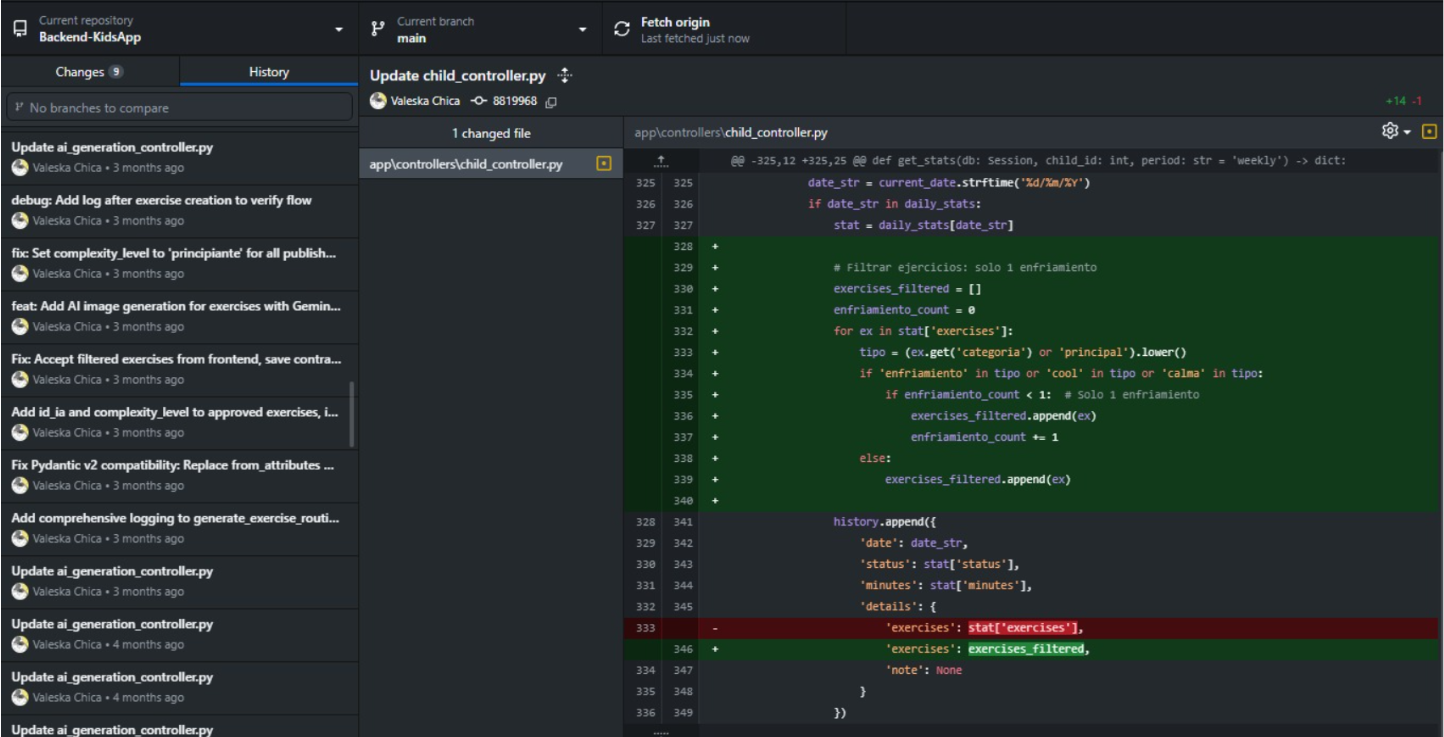
\includegraphics[width=\textwidth]{images/github_historial.png}
				\end{figure}
				\tblnote
				
			\subsection{Guion de entrevista}
				El guion de la entrevista utilizado para la recolección de información se presenta en los Anexos~3 y~4, donde se detallan las preguntas planteadas a los participantes según su perfil: especialistas en actividad física infantil y padres de familia~\cite{HernandezSampieri2014}. La estructura semiestructurada del guion permitió combinar preguntas predefinidas con la flexibilidad de explorar respuestas emergentes, enriqueciendo la información obtenida.
				
				Los ejes temáticos del guion fueron definidos a partir de la revisión de la literatura realizada en la fase inicial del proyecto, garantizando que las preguntas fueran pertinentes al contexto de uso del sistema y respondieran a necesidades identificadas en la evidencia científica~\cite{Creswell2018,HernandezSampieri2014}.
		
		\section{Desarrollo del sistema FitKids}
			En este apartado se describe el proceso de desarrollo del sistema FitKids, detallando las fases ejecutadas para la construcción de la aplicación móvil y de su infraestructura tecnológica de soporte. El desarrollo se condujo bajo la metodología \textit{Test-Driven Development Methodology for IoT-based Systems} (TDDM4IoTS), propuesta por Guerrero-Ulloa et al.~\cite{GuerreroUlloa2024} e integrada por los principios del desarrollo guiado por pruebas~\cite{Fowler2002}, la ingeniería dirigida por modelos~\cite{Kleppmann2017} y los enfoques ágiles, organizando el ciclo de vida en once fases que abarcan desde la recolección de requisitos hasta el mantenimiento del sistema.
			
			Cada fase de la metodología permitió identificar las necesidades de los usuarios, definir la arquitectura del sistema, implementar los distintos módulos funcionales y verificar su correcto funcionamiento, asegurando que la solución tecnológica cumpla con el objetivo de generar planes de ejercicios físicos personalizados y seguros para niños, alineados con las recomendaciones internacionales sobre actividad física infantil~\cite{Bull2020,Guthold2020}. El desarrollo consideró el uso de tecnologías móviles con evidencia de eficacia~\cite{Baumann2022} e inteligencia artificial generativa para la personalización de rutinas~\cite{Sengar2024}, con el fin de ofrecer una herramienta accesible, intuitiva y adaptable al contexto de cada usuario.
			
			\subsection{Fase 1: Recolección de datos iniciales}
				La fase de recolección de datos iniciales tuvo como objetivo obtener información relevante y contextualizada que permitió comprender la situación actual de la actividad física infantil, así como identificar necesidades, limitaciones y criterios clave para el diseño del sistema FitKids. Esta fase, denominada en TDDM4IoTS como \textit{preliminary analysis}~\cite{GuerreroUlloa2024}, constituyó la base para definir los requerimientos funcionales y no funcionales del sistema, asegurando que la solución tecnológica respondiera a criterios de seguridad, personalización y usabilidad~\cite{Hourcade2015}.
					
				Para la obtención de la información se empleó la técnica de la entrevista semiestructurada, dirigida a dos grupos de interés: especialistas en actividad física infantil y padres de familia de niños de 6 a 11 años. Las entrevistas se condujeron a partir de un guion semiestructurado, lo que permitió orientar la conversación hacia temas específicos sin limitar la posibilidad de obtener opiniones y experiencias detalladas, en línea con las buenas prácticas de elicitación de requisitos~\cite{HernandezSampieri2014,Creswell2018}. Para cada dimensión temática identificada en la revisión de la literatura se seleccionó al menos un artículo indexado que aportara evidencia empírica o normativa, a partir del cual se derivaron las preguntas correspondientes del guion; los artículos seleccionados y su aporte específico se detallan en la Tabla~\ref{tab:articulos_entrevista} de la sección de Resultados.
				
				En el caso de los especialistas, el guion se enfocó en su percepción sobre el nivel de actividad física infantil, las principales causas del sedentarismo, las consecuencias clínicas asociadas a la inactividad y las recomendaciones sobre tipo, duración e intensidad de las actividades adecuadas para los niños, contrastadas con las directrices de la OMS~\cite{Bull2020}. Asimismo, se indagó sobre los criterios clínicos para garantizar la seguridad de las rutinas y la opinión respecto al uso de aplicaciones móviles e inteligencia artificial como herramientas de apoyo~\cite{Yim2024,Direito2017}.
				
				Las entrevistas a padres permitieron recopilar información sobre los hábitos diarios de actividad física y uso de pantallas, las actividades más atractivas para los niños, las principales barreras que dificultan la práctica regular de ejercicio y los factores que influyen en su motivación~\cite{VegaDiaz2023,Yao2015}. Adicionalmente, se exploró el interés de los padres en el uso de aplicaciones móviles para el seguimiento de la actividad física y las funcionalidades que consideran necesarias en una herramienta orientada al bienestar infantil~\cite{Schoeppe2017}.
				
				La información obtenida permitió identificar patrones comunes, necesidades específicas y expectativas de ambos grupos. Estos insumos fueron fundamentales para orientar el diseño del sistema FitKids, definir sus módulos principales, establecer criterios de personalización de las rutinas y considerar los mecanismos de supervisión parental y seguridad, alineados con el objetivo general del proyecto y con la lógica iterativa propuesta por TDDM4IoTS~\cite{GuerreroUlloa2024,HernandezSampieri2014}.
					
			\subsection{Fase 2: Desarrollo del sistema}
				La Fase 2 corresponde al desarrollo del sistema FitKids, en la cual se materializa la solución tecnológica propuesta a partir de los requerimientos identificados en la fase previa. Conforme al esquema iterativo y ágil de TDDM4IoTS~\cite{GuerreroUlloa2024}, esta fase se descompone en diez subfases que cubren el ciclo de vida desde el diseño de la capa tecnológica hasta el mantenimiento del sistema desplegado, transformando el análisis preliminar en un sistema funcional mediante decisiones técnicas, de diseño y de arquitectura integradas.
					
				\subsubsection{Fase 2.1: Análisis preliminar.}
					En esta etapa se llevó a cabo un análisis orientado a definir los requisitos del sistema, seleccionar las tecnologías adecuadas y verificar la viabilidad del proyecto, en correspondencia con la fase de \textit{planning} reconocida explícitamente por TDDM4IoTS como elemento diferenciador frente a otras metodologías para sistemas IoT~\cite{GuerreroUlloa2024}. Este proceso se sustentó en la información obtenida durante la fase previa de recolección de datos, lo que permitió delimitar las necesidades funcionales y operativas del sistema. Las actividades realizadas se describen a continuación.
					
					\begin{itemize}
						\item \textbf{Análisis de requisitos:} se identificaron los requisitos funcionales y no funcionales a partir de la información recopilada en las entrevistas, siguiendo las prácticas estándar de la ingeniería de requisitos~\cite{Fowler2002}. Se establecieron las condiciones mínimas que debía cumplir la solución, incorporando criterios relacionados con la seguridad de las rutinas, la adecuación a la edad del niño, la facilidad de uso y la necesidad de supervisión por parte de los adultos. Los requisitos resultantes de este proceso se presentan en la sección de Resultados.
						\item \textbf{Análisis de tecnología:} se evaluaron diferentes alternativas tecnológicas considerando aspectos como compatibilidad, escalabilidad y facilidad de integración, siguiendo los principios de selección tecnológica recomendados para sistemas IoT~\cite{GuerreroUlloa2024,Kleppmann2017}. El resultado de este análisis comparativo se presenta en la sección de Resultados.
						\item \textbf{Análisis del entorno:} se examinaron las condiciones reales de uso del sistema, considerando el acceso a dispositivos móviles Android, el uso de navegadores web y la disponibilidad de conectividad, anticipando limitaciones operativas en concordancia con la actividad de \textit{environment analysis} de TDDM4IoTS~\cite{GuerreroUlloa2024}.
						\item \textbf{Análisis de viabilidad:} se evaluó la factibilidad del proyecto desde una perspectiva técnica, económica y operativa, contemplando los recursos disponibles y la posibilidad de integrar tecnologías externas~\cite{Creswell2018}. A partir de este análisis se determinó que la propuesta es viable dentro de las condiciones planteadas.
					\end{itemize}
					
				\subsubsection{Fase 2.2: Diseño de la capa tecnológica.}
					En esta etapa se definió la arquitectura general del sistema y se seleccionaron las tecnologías que lo soportarían, en correspondencia con la fase de \textit{technology layer design} de TDDM4IoTS~\cite{GuerreroUlloa2024}. La adopción de un enfoque multicapa con separación de responsabilidades constituye una práctica reconocida en arquitectura de software~\cite{Fowler2002}, especialmente apropiada para sistemas con interfaces heterogéneas y necesidades evolutivas como los basados en IoT~\cite{Kleppmann2017}.
					
					A partir de los requerimientos identificados se definieron cuatro capas: \textbf{presentación}, orientada a las interfaces de usuario con criterios de usabilidad y adaptación al contexto infantil~\cite{Hourcade2015,Nielsen1994}; \textbf{servicios de consumo}, basada en APIs REST por su flexibilidad e interoperabilidad~\cite{Kleppmann2017}; \textbf{negocio}, que encapsula la lógica central del sistema conforme al principio de separación de responsabilidades~\cite{Fowler2002}; y \textbf{datos}, soportada por un gestor de base de datos relacional en la nube que garantiza integridad, disponibilidad y seguridad~\cite{GuerreroUlloa2024}. Para cada componente del sistema se evaluaron múltiples alternativas tecnológicas considerando criterios de rendimiento, compatibilidad y escalabilidad; el resultado de este análisis comparativo se presenta en la sección de Resultados.
					
					El esquema de interacción entre capas se estableció de forma que las interfaces de usuario se comunican con la capa de servicios mediante solicitudes estructuradas, y esta a su vez gestiona la lógica del sistema y el acceso a los datos. Para representar esta arquitectura se emplearon herramientas de modelado en concordancia con la perspectiva de ingeniería dirigida por modelos asumida por TDDM4IoTS~\cite{GuerreroUlloa2024,Kleppmann2017}. La arquitectura resultante se presenta en la sección de Resultados.
					
				\subsubsection{Fase 2.3: Análisis detallado de requisitos.}
					En esta etapa, correspondiente a la fase de \textit{detailed requirement analysis} de TDDM4IoTS~\cite{GuerreroUlloa2024}, se realizó un análisis detallado con el propósito de precisar y refinar los aspectos identificados en las fases previas, estableciendo criterios técnicos y de calidad que orientarían el desarrollo posterior, alineados con los modelos de calidad de producto software~\cite{Fowler2002}.
					
					El análisis se sustentó en la información obtenida mediante las entrevistas, lo que facilitó contrastar los requerimientos iniciales con necesidades reales de uso~\cite{HernandezSampieri2014}. A partir de esta revisión se ajustaron aspectos relacionados con la seguridad de las actividades, la personalización de las rutinas y la facilidad de interacción del sistema, en consonancia con la evidencia sobre intervenciones digitales eficaces~\cite{Baumann2022,WangJun2024}.
					
					Los requerimientos se estructuraron de forma progresiva: primero los del backend, por su rol central en la gestión de la información y la lógica del sistema; a continuación los del entorno web, orientado a la gestión y validación de contenido; y finalmente los de la aplicación móvil, diferenciando los entornos de padres y modo niño, conforme al enfoque ágil incorporado por TDDM4IoTS~\cite{GuerreroUlloa2024}. Este enfoque permitió establecer una relación progresiva entre los componentes del sistema, evitando definir los módulos de forma aislada y facilitando su integración en fases posteriores. Los requisitos funcionales y no funcionales resultantes, junto con sus fichas de especificación detallada y criterios de aceptación, se presentan en la sección de Resultados.
					
				\subsubsection{Fase 2.4: Generación y adaptación de modelos.}
					En esta fase, denominada en TDDM4IoTS como \textit{model generation and adaptation}~\cite{GuerreroUlloa2024}, se desarrollaron y ajustaron los modelos necesarios para representar de forma estructurada el sistema. Conforme a los principios de la ingeniería dirigida por modelos~\cite{Kleppmann2017}, el modelado permitió anticipar el comportamiento del sistema y establecer una base conceptual coherente antes de su implementación, apoyándose en los requerimientos refinados en la fase anterior.
					
					El proceso se organizó de manera progresiva: se inició con la representación de la lógica central del sistema y se extendió hacia las interfaces, primero la web y posteriormente las móviles~\cite{GuerreroUlloa2024}. Se elaboraron diagramas de casos de uso, diagrama de clases, diagrama de despliegue y diagrama de componentes, los cuales permitieron validar conceptualmente el diseño, identificar posibles inconsistencias y asegurar la coherencia entre requerimientos, arquitectura y solución propuesta~\cite{Fowler2002}. Los modelos generados se presentan en la sección de Resultados.
					
				\subsubsection{Fase 2.5: Generación de pruebas.}
					Conforme al núcleo de TDDM4IoTS, las pruebas son definidas antes que el código, siguiendo el ciclo \textit{red-green-refactor} característico del desarrollo guiado por pruebas~\cite{Fowler2002,GuerreroUlloa2024}. En esta etapa se definieron los escenarios de prueba necesarios para verificar el comportamiento de los componentes, centrándose en establecer criterios de validación que permitieran detectar inconsistencias durante el desarrollo.
					
					La definición de las pruebas siguió una lógica progresiva alineada con las iteraciones de la metodología: primero las verificaciones sobre la lógica del backend mediante Pytest, luego los escenarios del entorno web con Vitest y React Testing Library, y finalmente los de la aplicación móvil con Jest y React Native Testing Library, diferenciando los contextos de padres y modo niño~\cite{GuerreroUlloa2024,Fowler2002}. Las pruebas de integración se plantearon para validar la interacción entre los distintos componentes del sistema, considerando el uso de TestClient de FastAPI con Pytest en el backend y herramientas de testing para la simulación de flujos completos en las interfaces~\cite{Fowler2002}. Los resultados de la ejecución de estas pruebas se presentan en la sección de Resultados.
					
				\subsubsection{Fase 2.6: Generación de software.}
					En esta fase, correspondiente a la \textit{software generation} de TDDM4IoTS~\cite{GuerreroUlloa2024}, se llevó a cabo el desarrollo del sistema mediante una implementación iterativa que permitió consolidar la integración de los componentes de manera controlada, conforme al carácter incremental promovido por las metodologías ágiles~\cite{Fowler2002}.
					
					El proceso se organizó en una secuencia lógica que inició con la lógica central del backend, estableciendo la base para la gestión de datos y la comunicación entre componentes; continuó con la integración del soporte de datos en la nube; y progresó hacia la aplicación web y finalmente la aplicación móvil, manteniendo coherencia entre módulos en línea con las prácticas de modularidad recomendadas en arquitectura de software~\cite{Fowler2002,Kleppmann2017}. Durante esta fase se incorporaron mecanismos de verificación continua sobre las funcionalidades implementadas y la interacción entre componentes, en concordancia con los ciclos cortos de retroalimentación propios de TDD~\cite{GuerreroUlloa2024,Fowler2002}. El software desarrollado y sus características técnicas se presentan en la sección de Resultados.
					
				\subsubsection{Fase 2.7: Refinamiento de modelos.}
					En esta fase, denominada \textit{model refinement} en TDDM4IoTS~\cite{GuerreroUlloa2024}, se realizó la revisión y ajuste de los modelos del sistema para mejorar su coherencia, escalabilidad y adaptación frente al desarrollo progresivo del sistema. El refinamiento se centró primero en los elementos asociados a la lógica central, luego en los modelos de la aplicación web y finalmente en los de la aplicación móvil, en consistencia con el flujo iterativo de la metodología~\cite{GuerreroUlloa2024}.
					
					Estos ajustes permitieron alinear los modelos con la implementación del sistema, reduciendo inconsistencias y fortaleciendo la estructura general~\cite{Fowler2002}. Los modelos refinados se presentan en la sección de Resultados junto con los modelos iniciales, permitiendo observar la evolución del diseño a lo largo del proceso.
					
				\subsubsection{Fase 2.8: Refinamiento de software.}
					En esta etapa, correspondiente al \textit{software refinement} de TDDM4IoTS~\cite{GuerreroUlloa2024}, se llevó a cabo la refactorización del código fuente con el propósito de mejorar su organización interna, legibilidad y capacidad de mantenimiento, sin alterar su comportamiento funcional, conforme a la definición canónica de refactorización~\cite{Fowler2002}.
					
					El refinamiento se realizó de manera progresiva: primero la lógica central, luego el entorno web y finalmente la aplicación móvil en ambos contextos de uso~\cite{GuerreroUlloa2024}. Estos ajustes permitieron reducir redundancias, mejorar la claridad del código y fortalecer la coherencia entre los distintos componentes, contribuyendo a los atributos de mantenibilidad y calidad interna del sistema~\cite{Fowler2002,Kleppmann2017}.
					
				\subsubsection{Fase 2.9: Despliegue del sistema.}
					En esta etapa, denominada \textit{hardware and software deployment} en TDDM4IoTS~\cite{GuerreroUlloa2024}, se realizó la configuración y publicación del sistema en entornos de producción. El proceso se llevó a cabo de forma progresiva: publicación del backend en Render, despliegue de la aplicación web, y distribución de la aplicación móvil mediante su publicación en Google Play Store, habilitando su instalación en dispositivos Android.
					
					Durante esta fase se verificó la compatibilidad del sistema en distintos navegadores y dispositivos móviles, así como la correcta comunicación entre el backend, las interfaces de usuario y la base de datos, atendiendo a los atributos de portabilidad y compatibilidad descritos en los modelos de calidad~\cite{GuerreroUlloa2024}. Este proceso permitió disponer de una versión operativa del sistema, preparada para su validación en condiciones reales de uso.
					
				\subsubsection{Fase 2.10: Evaluación de entregables.}
					Esta fase corresponde al \textit{deliverable assessment} de TDDM4IoTS~\cite{GuerreroUlloa2024}. Cada entregable fue evaluado por la autora al culminar su implementación; cuando cumplió con los requisitos definidos, fue evaluado también por usuarios directos: el backend por el director del proyecto, la aplicación web por un profesional de pediatría, y la aplicación móvil por dos padres de familia y sus hijos en edades correspondientes al rango objetivo. Estas evaluaciones directas sirvieron para ajustar el funcionamiento y la interacción a las necesidades de los usuarios reales.
					
					Una vez desplegado el sistema, se evaluó su comportamiento en condiciones reales de uso y su correspondencia con los requerimientos establecidos, en línea con las dimensiones de calidad de producto software definidas por la norma ISO/IEC 25010~\cite{ISO25010,GuerreroUlloa2024}. El enfoque de evaluación se organizó progresivamente: primero los componentes de gestión del sistema, luego los entornos de supervisión y finalmente los escenarios de interacción directa con el usuario final~\cite{GuerreroUlloa2024,Nielsen1994}. Se definieron criterios de funcionalidad, usabilidad, aceptación y consistencia, considerando especialmente las particularidades del usuario infantil~\cite{Hourcade2015,Bangor2009}. Los resultados obtenidos se presentan en detalle en la sección de Resultados.
					
				\subsubsection{Fase 2.11: Mantenimiento.}
					Al tratarse de un prototipo, el sistema FitKids no ha contemplado hasta el momento actividades de mantenimiento sustantivas, aunque la metodología TDDM4IoTS reconoce explícitamente esta fase como parte integral de su ciclo de vida~\cite{GuerreroUlloa2024}. El carácter modular y por capas del sistema garantiza que las actividades de mantenimiento futuras sean accesibles y manejables, atributo directamente relacionado con la dimensión de mantenibilidad de los modelos de calidad de software~\cite{Fowler2002}. Estas actividades podrán incluir tareas correctivas, adaptativas y evolutivas orientadas a asegurar la adaptación del sistema a futuras necesidades.
					
		\section{Cronograma}
			El cronograma de actividades permitió planificar y organizar las tareas del proyecto tecnológico FitKids a lo largo de los semestres noveno y décimo, considerando los cortes académicos establecidos por la institución~\cite{GuerreroUlloa2024}. La distribución de actividades respondió a la lógica iterativa de TDDM4IoTS, estableciendo una progresión coherente desde la conceptualización del problema hasta la entrega y predefensa del sistema desarrollado. La Figura~\ref{fig:cronograma} presenta el diagrama de Gantt correspondiente.
			
			\begin{figure}[H]
				\centering
				\caption{Cronograma de actividades del proyecto tecnológico FitKids}
				\label{fig:cronograma}
				\resizebox{\textwidth}{!}{%
					\begin{tikzpicture}[font=\tiny, line width=0.3pt]
						\def\AW{3.2}
						\def\CW{0.33}
						% R0 yellow header
						\fill[hYellow] (0,0) rectangle (\AW+40*\CW,-0.45);
						% R1 white numbers
						\fill[white] (0,-0.45) rectangle (\AW+40*\CW,-0.85);
						% R2 blue cortes
						\fill[hBlue] (0,-0.85) rectangle (\AW+40*\CW,-1.25);
						% R3 blue anteproyecto
						\fill[hBlue] (0,-1.25) rectangle (\AW+40*\CW,-1.65);
						% Activity rows
						\fill[aGreen](0,-1.65) rectangle (\AW,-2.15);
						\fill[white](\AW,-1.65) rectangle (\AW+40*\CW,-2.15);
						\fill[aGreen](0,-2.15) rectangle (\AW,-3.00);
						\fill[white](\AW,-2.15) rectangle (\AW+40*\CW,-3.00);
						\fill[aGreen](0,-3.00) rectangle (\AW,-3.55);
						\fill[white](\AW,-3.00) rectangle (\AW+40*\CW,-3.55);
						\fill[aGreen](0,-3.55) rectangle (\AW,-4.10);
						\fill[white](\AW,-3.55) rectangle (\AW+40*\CW,-4.10);
						\fill[aGreen](0,-4.10) rectangle (\AW,-4.65);
						\fill[white](\AW,-4.10) rectangle (\AW+40*\CW,-4.65);
						\fill[aGreen](0,-4.65) rectangle (\AW,-5.20);
						\fill[white](\AW,-4.65) rectangle (\AW+40*\CW,-5.20);
						\fill[aGreen](0,-5.20) rectangle (\AW,-5.75);
						\fill[white](\AW,-5.20) rectangle (\AW+40*\CW,-5.75);
						\fill[aGreen](0,-5.75) rectangle (\AW,-6.30);
						\fill[white](\AW,-5.75) rectangle (\AW+40*\CW,-6.30);
						\fill[aGreen](0,-6.30) rectangle (\AW,-7.00);
						\fill[white](\AW,-6.30) rectangle (\AW+40*\CW,-7.00);
						\fill[aGreen](0,-7.00) rectangle (\AW,-7.70);
						\fill[white](\AW,-7.00) rectangle (\AW+40*\CW,-7.70);
						\fill[aGreen](0,-7.70) rectangle (\AW,-8.25);
						\fill[white](\AW,-7.70) rectangle (\AW+40*\CW,-8.25);
						% Gantt bars
						\fill[barC](\AW+0*\CW,-1.65) rectangle (\AW+2*\CW,-2.15);
						\fill[barC](\AW+2*\CW,-2.15) rectangle (\AW+5*\CW,-3.00);
						\fill[barC](\AW+4*\CW,-3.00) rectangle (\AW+7*\CW,-3.55);
						\fill[barC](\AW+7*\CW,-3.55) rectangle (\AW+9*\CW,-4.10);
						\fill[barC](\AW+9*\CW,-4.10) rectangle (\AW+13*\CW,-4.65);
						\fill[barC](\AW+11*\CW,-4.65) rectangle (\AW+15*\CW,-5.20);
						\fill[barC](\AW+22*\CW,-5.20) rectangle (\AW+27*\CW,-5.75);
						\fill[barC](\AW+25*\CW,-5.75) rectangle (\AW+30*\CW,-6.30);
						\fill[barC](\AW+30*\CW,-6.30) rectangle (\AW+34*\CW,-7.00);
						\fill[barC](\AW+34*\CW,-7.00) rectangle (\AW+37*\CW,-7.70);
						\fill[barC](\AW+37*\CW,-7.70) rectangle (\AW+38*\CW,-8.25);
						% Horizontal lines
						\draw[black](0,0)--(\AW+40*\CW,0);
						\draw[black](0,-0.45)--(\AW+40*\CW,-0.45);
						\draw[black](0,-0.85)--(\AW+40*\CW,-0.85);
						\draw[black](0,-1.25)--(\AW+40*\CW,-1.25);
						\draw[black](0,-1.65)--(\AW+40*\CW,-1.65);
						\draw[black](0,-2.15)--(\AW+40*\CW,-2.15);
						\draw[black](0,-3.00)--(\AW+40*\CW,-3.00);
						\draw[black](0,-3.55)--(\AW+40*\CW,-3.55);
						\draw[black](0,-4.10)--(\AW+40*\CW,-4.10);
						\draw[black](0,-4.65)--(\AW+40*\CW,-4.65);
						\draw[black](0,-5.20)--(\AW+40*\CW,-5.20);
						\draw[black](0,-5.75)--(\AW+40*\CW,-5.75);
						\draw[black](0,-6.30)--(\AW+40*\CW,-6.30);
						\draw[black](0,-7.00)--(\AW+40*\CW,-7.00);
						\draw[black](0,-7.70)--(\AW+40*\CW,-7.70);
						\draw[black](0,-8.25)--(\AW+40*\CW,-8.25);
						% Vertical borders
						\draw[black,line width=0.8pt](0,0)--(0,-8.25);
						\draw[black,line width=0.8pt](\AW,0)--(\AW,-8.25);
						\draw[black,line width=1.0pt](\AW+20*\CW,0)--(\AW+20*\CW,-8.25);
						\draw[black,line width=0.8pt](\AW+40*\CW,0)--(\AW+40*\CW,-8.25);
						% Vertical week grid lines
						\draw[grayBorder](\AW+1*\CW,-0.45)--(\AW+1*\CW,-8.25);
						\draw[grayBorder](\AW+2*\CW,-0.45)--(\AW+2*\CW,-8.25);
						\draw[grayBorder](\AW+3*\CW,-0.45)--(\AW+3*\CW,-8.25);
						\draw[grayBorder](\AW+4*\CW,-0.45)--(\AW+4*\CW,-8.25);
						\draw[grayBorder](\AW+5*\CW,-0.45)--(\AW+5*\CW,-8.25);
						\draw[grayBorder](\AW+6*\CW,-0.45)--(\AW+6*\CW,-8.25);
						\draw[grayBorder](\AW+7*\CW,-0.45)--(\AW+7*\CW,-8.25);
						\draw[grayBorder](\AW+8*\CW,-0.45)--(\AW+8*\CW,-8.25);
						\draw[grayBorder](\AW+9*\CW,-0.45)--(\AW+9*\CW,-8.25);
						\draw[grayBorder](\AW+10*\CW,-0.45)--(\AW+10*\CW,-8.25);
						\draw[grayBorder](\AW+11*\CW,-0.45)--(\AW+11*\CW,-8.25);
						\draw[grayBorder](\AW+12*\CW,-0.45)--(\AW+12*\CW,-8.25);
						\draw[grayBorder](\AW+13*\CW,-0.45)--(\AW+13*\CW,-8.25);
						\draw[grayBorder](\AW+14*\CW,-0.45)--(\AW+14*\CW,-8.25);
						\draw[grayBorder](\AW+15*\CW,-0.45)--(\AW+15*\CW,-8.25);
						\draw[grayBorder](\AW+16*\CW,-0.45)--(\AW+16*\CW,-8.25);
						\draw[grayBorder](\AW+17*\CW,-0.45)--(\AW+17*\CW,-8.25);
						\draw[grayBorder](\AW+18*\CW,-0.45)--(\AW+18*\CW,-8.25);
						\draw[grayBorder](\AW+19*\CW,-0.45)--(\AW+19*\CW,-8.25);
						\draw[grayBorder](\AW+21*\CW,-0.45)--(\AW+21*\CW,-8.25);
						\draw[grayBorder](\AW+22*\CW,-0.45)--(\AW+22*\CW,-8.25);
						\draw[grayBorder](\AW+23*\CW,-0.45)--(\AW+23*\CW,-8.25);
						\draw[grayBorder](\AW+24*\CW,-0.45)--(\AW+24*\CW,-8.25);
						\draw[grayBorder](\AW+25*\CW,-0.45)--(\AW+25*\CW,-8.25);
						\draw[grayBorder](\AW+26*\CW,-0.45)--(\AW+26*\CW,-8.25);
						\draw[grayBorder](\AW+27*\CW,-0.45)--(\AW+27*\CW,-8.25);
						\draw[grayBorder](\AW+28*\CW,-0.45)--(\AW+28*\CW,-8.25);
						\draw[grayBorder](\AW+29*\CW,-0.45)--(\AW+29*\CW,-8.25);
						\draw[grayBorder](\AW+30*\CW,-0.45)--(\AW+30*\CW,-8.25);
						\draw[grayBorder](\AW+31*\CW,-0.45)--(\AW+31*\CW,-8.25);
						\draw[grayBorder](\AW+32*\CW,-0.45)--(\AW+32*\CW,-8.25);
						\draw[grayBorder](\AW+33*\CW,-0.45)--(\AW+33*\CW,-8.25);
						\draw[grayBorder](\AW+34*\CW,-0.45)--(\AW+34*\CW,-8.25);
						\draw[grayBorder](\AW+35*\CW,-0.45)--(\AW+35*\CW,-8.25);
						\draw[grayBorder](\AW+36*\CW,-0.45)--(\AW+36*\CW,-8.25);
						\draw[grayBorder](\AW+37*\CW,-0.45)--(\AW+37*\CW,-8.25);
						\draw[grayBorder](\AW+38*\CW,-0.45)--(\AW+38*\CW,-8.25);
						\draw[grayBorder](\AW+39*\CW,-0.45)--(\AW+39*\CW,-8.25);
						% Corte dividers
						\draw[grayBorder](\AW+10*\CW,-0.85)--(\AW+10*\CW,-1.65);
						\draw[grayBorder](\AW+30*\CW,-0.85)--(\AW+30*\CW,-1.65);
						% Headers R0
						\node[anchor=center,font=\tiny\bfseries] at (\AW/2,-0.225) {Semana};
						\node[anchor=center,font=\tiny\bfseries] at (\AW+10*\CW,-0.225) {9no semestre};
						\node[anchor=center,font=\tiny\bfseries] at (\AW+30*\CW,-0.225) {10mo semestre};
						% Week numbers R1
						\node[anchor=center,font=\tiny] at (\AW+0.5*\CW,-0.65) {1};
						\node[anchor=center,font=\tiny] at (\AW+1.5*\CW,-0.65) {2};
						\node[anchor=center,font=\tiny] at (\AW+2.5*\CW,-0.65) {3};
						\node[anchor=center,font=\tiny] at (\AW+3.5*\CW,-0.65) {4};
						\node[anchor=center,font=\tiny] at (\AW+4.5*\CW,-0.65) {5};
						\node[anchor=center,font=\tiny] at (\AW+5.5*\CW,-0.65) {6};
						\node[anchor=center,font=\tiny] at (\AW+6.5*\CW,-0.65) {7};
						\node[anchor=center,font=\tiny] at (\AW+7.5*\CW,-0.65) {8};
						\node[anchor=center,font=\tiny] at (\AW+8.5*\CW,-0.65) {9};
						\node[anchor=center,font=\tiny] at (\AW+9.5*\CW,-0.65) {10};
						\node[anchor=center,font=\tiny] at (\AW+10.5*\CW,-0.65) {11};
						\node[anchor=center,font=\tiny] at (\AW+11.5*\CW,-0.65) {12};
						\node[anchor=center,font=\tiny] at (\AW+12.5*\CW,-0.65) {13};
						\node[anchor=center,font=\tiny] at (\AW+13.5*\CW,-0.65) {14};
						\node[anchor=center,font=\tiny] at (\AW+14.5*\CW,-0.65) {15};
						\node[anchor=center,font=\tiny] at (\AW+15.5*\CW,-0.65) {16};
						\node[anchor=center,font=\tiny] at (\AW+16.5*\CW,-0.65) {17};
						\node[anchor=center,font=\tiny] at (\AW+17.5*\CW,-0.65) {18};
						\node[anchor=center,font=\tiny] at (\AW+18.5*\CW,-0.65) {19};
						\node[anchor=center,font=\tiny] at (\AW+19.5*\CW,-0.65) {20};
						\node[anchor=center,font=\tiny] at (\AW+20.5*\CW,-0.65) {1};
						\node[anchor=center,font=\tiny] at (\AW+21.5*\CW,-0.65) {2};
						\node[anchor=center,font=\tiny] at (\AW+22.5*\CW,-0.65) {3};
						\node[anchor=center,font=\tiny] at (\AW+23.5*\CW,-0.65) {4};
						\node[anchor=center,font=\tiny] at (\AW+24.5*\CW,-0.65) {5};
						\node[anchor=center,font=\tiny] at (\AW+25.5*\CW,-0.65) {6};
						\node[anchor=center,font=\tiny] at (\AW+26.5*\CW,-0.65) {7};
						\node[anchor=center,font=\tiny] at (\AW+27.5*\CW,-0.65) {8};
						\node[anchor=center,font=\tiny] at (\AW+28.5*\CW,-0.65) {9};
						\node[anchor=center,font=\tiny] at (\AW+29.5*\CW,-0.65) {10};
						\node[anchor=center,font=\tiny] at (\AW+30.5*\CW,-0.65) {11};
						\node[anchor=center,font=\tiny] at (\AW+31.5*\CW,-0.65) {12};
						\node[anchor=center,font=\tiny] at (\AW+32.5*\CW,-0.65) {13};
						\node[anchor=center,font=\tiny] at (\AW+33.5*\CW,-0.65) {14};
						\node[anchor=center,font=\tiny] at (\AW+34.5*\CW,-0.65) {15};
						\node[anchor=center,font=\tiny] at (\AW+35.5*\CW,-0.65) {16};
						\node[anchor=center,font=\tiny] at (\AW+36.5*\CW,-0.65) {17};
						\node[anchor=center,font=\tiny] at (\AW+37.5*\CW,-0.65) {18};
						\node[anchor=center,font=\tiny] at (\AW+38.5*\CW,-0.65) {19};
						\node[anchor=center,font=\tiny] at (\AW+39.5*\CW,-0.65) {20};
						% Cortes R2
						\node[anchor=center,font=\tiny\bfseries] at (\AW+5*\CW,-1.05) {corte 1};
						\node[anchor=center,font=\tiny\bfseries] at (\AW+15*\CW,-1.05) {corte 2};
						\node[anchor=center,font=\tiny\bfseries] at (\AW+25*\CW,-1.05) {corte 1};
						\node[anchor=center,font=\tiny\bfseries] at (\AW+35*\CW,-1.05) {corte 2};
						% Anteproyecto R3
						\node[anchor=center,font=\tiny\bfseries] at (\AW/2,-1.45) {Anteproyecto};
						\node[anchor=center,font=\tiny] at (\AW+5*\CW,-1.45) {Anteproyecto};
						\node[anchor=center,font=\tiny] at (\AW+15*\CW,-1.45) {obj1, obj2, avance del obj3};
						\node[anchor=center,font=\tiny] at (\AW+25*\CW,-1.45) {fin obj3, avance del obj4};
						\node[anchor=center,font=\tiny] at (\AW+35*\CW,-1.45) {fin obj4, Relaccion y tramites};
						% Activity labels
						\node[anchor=center,align=center,font=\tiny] at (\AW/2,-1.90) {Concepci\'on del Proyecto};
						\node[anchor=center,align=center,font=\tiny] at (\AW/2,-2.575) {Definici\'on de Objetivos,\\problem\'atica y\\justificaci\'on};
						\node[anchor=center,align=center,font=\tiny] at (\AW/2,-3.275) {Definici\'on del marco\\te\'orico y referencial};
						\node[anchor=center,align=center,font=\tiny] at (\AW/2,-3.825) {Formulaci\'on de\\resultados esperados};
						\node[anchor=center,align=center,font=\tiny] at (\AW/2,-4.375) {revisi\'on de la literatura};
						\node[anchor=center,align=center,font=\tiny] at (\AW/2,-4.925) {Dise\~no de Interfaces};
						\node[anchor=center,align=center,font=\tiny] at (\AW/2,-5.475) {Desarrollo del Backend};
						\node[anchor=center,align=center,font=\tiny] at (\AW/2,-6.025) {Desarrollo del Frontend};
						\node[anchor=center,align=center,font=\tiny] at (\AW/2,-6.65) {Integraci\'on del sistema\\y pruebas};
						\node[anchor=center,align=center,font=\tiny] at (\AW/2,-7.35) {Correcci\'on del proyecto\\y entrega final};
						\node[anchor=center,align=center,font=\tiny] at (\AW/2,-7.975) {Predefensa del proyecto};
				\end{tikzpicture}}
				
			\end{figure}
			\tblnote
			
			Como se observa en la Figura~\ref{fig:cronograma}, durante el noveno semestre se ejecutaron las actividades correspondientes a la fase de anteproyecto y conceptualización: concepción del proyecto (semanas 1--2), definición de objetivos, problemática y justificación (semanas 3--5), definición del marco teórico y referencial (semanas 5--7), formulación de resultados esperados (semanas 8--9) y revisión de la literatura (semanas 10--13). Estas actividades se distribuyeron en dos cortes académicos: el primero cubrió los objetivos iniciales y el avance del tercer objetivo, mientras que el segundo completó los objetivos restantes y los trámites previos al inicio del desarrollo.
			
			Durante el décimo semestre se ejecutaron las actividades de implementación del sistema: diseño de interfaces (semanas 11--14 del 9no semestre y primeras semanas del 10mo), desarrollo del backend (semanas 3--7), desarrollo del frontend (semanas 6--10), integración del sistema y pruebas (semanas 11--14), corrección del proyecto y entrega final (semanas 15--18), y predefensa del proyecto (últimos días de la semana 18). Esta organización garantizó que cada componente del sistema fuera desarrollado, integrado y validado antes de avanzar a la siguiente etapa, en coherencia con el enfoque iterativo propuesto por la metodología TDDM4IoTS~\cite{GuerreroUlloa2024,Fowler2002}.
		
		
		\section{Indicadores de evaluación}
			De acuerdo con el reglamento institucional para el Proyecto Tecnológico de la Unidad de Integración Curricular de la Universidad Técnica Estatal de Quevedo, esta sección describe las pruebas a las que fue sometido el sistema, presenta el análisis crítico del producto obtenido y registra las modificaciones y mejoras adoptadas durante el proceso de verificación y validación~\cite{GuerreroUlloa2024}. Los indicadores reportados se seleccionaron entre los recomendados por el reglamento ---cumplimiento de cronograma, presupuesto, alcance, calidad del producto, satisfacción del usuario, adopción tecnológica, rendimiento y mantenibilidad--- y se complementaron con instrumentos validados para evaluar específicamente un sistema de salud digital orientado al público infantil~\cite{Bangor2009,Venkatesh2003}.
			
			La evaluación contempla dos planos articulados: un plano de \textbf{verificación}, dirigido a comprobar que el producto cumple con las especificaciones técnicas y funcionales declaradas, y un plano de \textbf{validación}, orientado a confirmar que el sistema satisface las necesidades reales de los usuarios finales y resuelve el problema planteado~\cite{GuerreroUlloa2024}. Esta distinción es coherente con el modelo de calidad de producto de software propuesto por la norma ISO/IEC 25010 \cite{ISO25010}, que separa la calidad interna y externa del producto de la calidad en uso percibida por sus usuarios~\cite{GuerreroUlloa2024}, y se alinea con la fase de evaluación de entregables establecida por la metodología TDDM4IoTS adoptada en el presente proyecto.
			
			\subsection{Categorías de indicadores adoptadas}
				Para una evaluación integral del proyecto se adoptan tres categorías complementarias de indicadores, cuya elección obedece tanto a las directrices del reglamento institucional como a la naturaleza del producto desarrollado~\cite{GuerreroUlloa2024,Fowler2002}:
				
				\begin{itemize}
					\item \textbf{Indicadores de gestión del proyecto:} comprenden el cumplimiento del alcance, del cronograma y del presupuesto, en correspondencia con las prácticas estándar de gestión de proyectos~\cite{Creswell2018}.
					\item \textbf{Indicadores de calidad técnica del producto:} evalúan los atributos funcionales y no funcionales del software ---funcionalidad, fiabilidad, eficiencia, mantenibilidad y seguridad--- tomando como referencia la norma ISO/IEC 25010~\cite{GuerreroUlloa2024} y operacionalizándolos mediante pruebas unitarias, pruebas de integración y verificación del cumplimiento de requisitos~\cite{Fowler2002}.
					\item \textbf{Indicadores de calidad en uso:} miden la aceptación, la usabilidad y la pertinencia del sistema desde la perspectiva de los usuarios finales mediante instrumentos validados como el Modelo de Aceptación Tecnológica (TAM)~\cite{Venkatesh2003} y la Escala de Usabilidad del Sistema (SUS)~\cite{Bangor2009}.
				\end{itemize}
				
			\subsection{Instrumentos de medición y formalización matemática}
				Cada indicador se evalúa mediante un instrumento específico, acorde con el aspecto analizado del sistema FitKids, y se cuantifica con una expresión matemática que permite obtener un valor objetivo y verificable~\cite{GuerreroUlloa2024}. Las ecuaciones se presentan numeradas consecutivamente conforme al formato institucional, y los símbolos empleados se definen inmediatamente después de cada expresión.
				
				\subsubsection{Cumplimiento de requisitos (CR).}
					La verificación del alcance del sistema se realiza mediante una matriz de trazabilidad que vincula cada requisito con los componentes desarrollados y con las pruebas que lo validan~\cite{Fowler2002}. El cumplimiento de requisitos se calcula como:
					
					\begin{equation}
						\label{ec:cr}
						CR = \frac{R_c}{R_t} \times 100
					\end{equation}
					
					donde $CR$ es el porcentaje de cumplimiento de requisitos; $R_c$ es el número de requisitos cubiertos y verificados; y $R_t$ es el número total de requisitos definidos en la fase de análisis. El criterio de aceptación adoptado es $CR \geq 95\%$, en línea con las prácticas habituales de aseguramiento de calidad en proyectos de ingeniería de software~\cite{Fowler2002}.
					
				\subsubsection{Variación del cronograma (VC) e índice SPI.}
					La puntualidad de la ejecución se evalúa mediante un diagrama de Gantt comparativo que confronta la planificación inicial con la ejecución real~\cite{GuerreroUlloa2024}. Para cuantificar la desviación se calcula la variación del cronograma ($VC$) y el índice de desempeño del cronograma ($SPI$):
					
					\begin{equation}
						\label{ec:vc}
						VC = \frac{T_r - T_p}{T_p} \times 100\%
					\end{equation}
					
					\begin{equation}
						\label{ec:spi}
						SPI = \frac{T_p}{T_r}
					\end{equation}
					
					donde $T_p$ es la duración planificada del proyecto (en días) y $T_r$ es la duración realmente ejecutada. Un valor de $VC$ positivo indica retraso; un valor negativo indica adelanto. El índice $SPI$ toma valores menores que 1 cuando la ejecución va por detrás del plan, igual a 1 cuando coincide, y mayor que 1 cuando el proyecto se ejecuta más rápido. Se establece como criterio de aceptación $|VC| \leq 10\%$ y $SPI \geq 0{,}9$~\cite{Creswell2018}.
					
				\subsubsection{Variación del presupuesto (VP) e índice CPI.}
					El control financiero se evalúa comparando el costo proyectado con el costo realmente incurrido, conforme al formato sugerido por el reglamento~\cite{GuerreroUlloa2024}. Se aplican dos métricas complementarias:
					
					\begin{equation}
						\label{ec:vp}
						VP = \frac{C_r - C_p}{C_p} \times 100\%
					\end{equation}
					
					\begin{equation}
						\label{ec:cpi}
						CPI = \frac{C_p}{C_r}
					\end{equation}
					
					donde $C_p$ es el costo planificado del proyecto (en USD) y $C_r$ es el costo real ejecutado al cierre. Un valor de $VP$ positivo indica sobrecosto; un valor negativo indica ahorro. El índice $CPI$ toma valores menores que 1 cuando se ha consumido más recursos de los previstos, igual a 1 cuando el costo real coincide con el planificado, y mayor que 1 cuando el trabajo se ha ejecutado por debajo del costo planificado. Se establece como criterio de aceptación $|VP| \leq 10\%$ y $CPI \geq 0{,}9$.
			
				\subsubsection{Cobertura de pruebas (CP).}
					La calidad técnica del producto se mide mediante la ejecución de pruebas unitarias y de integración, orientadas a verificar la funcionalidad, la fiabilidad y la eficiencia del software según el modelo de calidad ISO/IEC 25010~\cite{GuerreroUlloa2024}. La cobertura de pruebas se calcula como:
					
					\begin{equation}
						\label{ec:cp}
						CP = \frac{N_a}{N_t} \times 100\%
					\end{equation}
					
					donde $CP$ es la cobertura de pruebas expresada en porcentaje; $N_a$ es el número de pruebas aprobadas; y $N_t$ es el número total de pruebas ejecutadas. Se establece como criterio de aceptación $CP \geq 90\%$, valor consistente con la fase de generación y ejecución de pruebas de TDDM4IoTS~\cite{GuerreroUlloa2024,Fowler2002}.
			
				\subsubsection{Aceptación tecnológica (TAM).}
					Para evaluar la aceptación del sistema por parte de los padres de familia se aplica el Modelo de Aceptación Tecnológica (TAM), que mide la utilidad percibida y la facilidad de uso percibida mediante una escala Likert de cinco puntos~\cite{Venkatesh2003,Davis1989}. La puntuación media del instrumento se calcula como:
					
					\begin{equation}
						\label{ec:TAM}
						\bar{X}_{TAM} = \frac{1}{n} \sum_{i=1}^{n} x_i
					\end{equation}
					
					donde $\bar{X}_{TAM}$ es la puntuación media del cuestionario TAM; $x_i$ es la respuesta del $i$-ésimo participante en escala 1--5; y $n$ es el número total de respuestas válidas. Se considera satisfactoria una puntuación media $\bar{X}_{TAM} \geq 4{,}0$, valor que indica una percepción positiva mayoritaria sobre la utilidad y la facilidad de uso del sistema~\cite{Venkatesh2003}.
			
				\subsubsection{Usabilidad infantil (SUS).}
					La usabilidad del modo niño se evalúa mediante la Escala de Usabilidad del Sistema (SUS), aplicada con el acompañamiento de los representantes legales y considerando las adaptaciones recomendadas para su uso con menores de edad~\cite{Bangor2009,Hourcade2015}. El instrumento consta de diez ítems con escala Likert 1--5, alternando entre afirmaciones positivas (ítems impares) y negativas (ítems pares). La puntuación se calcula con la fórmula original propuesta por Brooke~\cite{Brooke1996}:
					
					\begin{equation}
						\label{ec:SUS}
						SUS = 2{,}5 \cdot \left[\sum_{i} (P_i - 1) + \sum_{i} (5 - I_i)\right]
					\end{equation}
					
					donde $SUS$ es la puntuación final expresada en escala de 0 a 100; $P_i$ es la respuesta del usuario al ítem par $i$; e $I_i$ es la respuesta al ítem impar $i$. Conforme a los rangos empíricos publicados, una puntuación $SUS \geq 68$ corresponde a usabilidad aceptable y se establece como criterio de aceptación para este indicador~\cite{Bangor2009}.
			
				\subsubsection{Validación clínica.}
					La pertinencia clínica y la seguridad de las rutinas generadas por el sistema se evalúan mediante un análisis cualitativo conducido por una pediatra colaboradora, quien aplica observación directa y emite comentarios profesionales sobre la adecuación de las actividades a los rangos de edad, el cumplimiento de las recomendaciones de actividad física infantil y la organización general de la información~\cite{Bull2020,Yim2024}. Por su naturaleza cualitativa, este indicador no se cuantifica mediante una expresión matemática, sino que se documenta mediante el registro estructurado de observaciones, en línea con la práctica de evaluación heurística complementaria a las pruebas con usuarios~\cite{Nielsen1994}. El criterio de aceptación adoptado es la ausencia de objeciones críticas relacionadas con la seguridad de las rutinas.
			
				\subsubsection{Rendimiento del sistema.}
					El rendimiento del sistema se evalúa mediante pruebas de carga sobre la API REST y la aplicación móvil, registrando el tiempo de respuesta de las operaciones críticas del sistema: autenticación, generación de rutinas mediante inteligencia artificial generativa y consulta de progreso del niño~\cite{GuerreroUlloa2024,Fowler2002}. Dado que FitKids integra una API externa de IA generativa (Gemini) cuya latencia es estructuralmente mayor a la de las operaciones propias del sistema, se definen dos indicadores de rendimiento diferenciados que permiten una evaluación más precisa y defendible de la eficiencia del sistema~\cite{Yu2020}.
					
					El tiempo medio de respuesta para cada categoría de operación se calcula como:
					
					\begin{equation}
						\label{ec:tr}
						\bar{T} = \frac{1}{n} \sum_{i=1}^{n} t_i
					\end{equation}
					
					donde $\bar{T}$ es el tiempo medio de respuesta del sistema expresado en milisegundos; $t_i$ es el tiempo de respuesta registrado en la $i$-ésima ejecución de la operación evaluada; y $n$ es el número total de ejecuciones registradas para esa operación.
					
					Se establecen dos criterios de aceptación diferenciados conforme a la naturaleza de cada operación. Para las \textbf{operaciones estándar} ---autenticación e inicio de sesión, consulta de progreso y configuración de recordatorios--- se adopta el criterio $\bar{T}_{est} \leq 1\,000\,\text{ms}$, límite dentro del cual el flujo de interacción del usuario permanece ininterrumpido según los umbrales clásicos de tiempo de respuesta en sistemas interactivos~\cite{Nielsen1994}, confirmados empíricamente para aplicaciones móviles por Yu et al.~\cite{Yu2020}, quienes demostraron que tiempos de respuesta superiores a este umbral producen una degradación significativa en la tolerancia, aceptación y satisfacción del usuario. Para la \textbf{generación de rutinas mediante IA generativa}, cuya latencia depende de una llamada a la API externa de Gemini y está fuera del control directo del sistema, se adopta el criterio $\bar{T}_{IA} \leq 10\,000\,\text{ms}$, umbral hasta el cual el usuario mantiene la atención sobre la tarea cuando el sistema provee retroalimentación visual del proceso en curso~\cite{Nielsen1994}. Ambos criterios son coherentes con la dimensión de eficiencia de desempeño definida por la norma ISO/IEC~25010~\cite{GuerreroUlloa2024}.
			
			\subsection{Síntesis de los indicadores adoptados}
				La Tabla~\ref{tab:indicadores} sintetiza los indicadores adoptados, el aspecto del sistema que cada uno evalúa, el instrumento empleado, la ecuación asociada y el criterio de aceptación definido para considerar satisfactorio el resultado.
				
				\begingroup
				\setlength{\LTpre}{6pt}\setlength{\LTpost}{2pt}
				\renewcommand{\arraystretch}{1.15}
				\small
				\begin{longtable}{p{2.3cm}p{2.95cm}p{3cm}p{1.5cm}p{3.75cm}}
					\caption{Indicadores de evaluación del sistema FitKids}\label{tab:indicadores}\\
					\hline
					\textbf{Indicador} & \textbf{Aspecto evaluado} & \textbf{Instrumento} & \textbf{Ecuación} & \textbf{Criterio de aceptación}\\
					\hline
					\endfirsthead
					\hline
					\textbf{Indicador} & \textbf{Aspecto evaluado} & \textbf{Instrumento} & \textbf{Ecuación} & \textbf{Criterio de aceptación}\\
					\hline
					\endhead
					\hline
					\multicolumn{5}{r}{\footnotesize\itshape continúa $\rightarrow$}\\
					\endfoot
					\hline
					\endlastfoot
					Cumplimiento de requisitos & Alcance funcional y no funcional & Matriz de trazabilidad de requisitos & \eqref{ec:cr} & $CR \geq 95\%$\\
					Variación del cronograma & Puntualidad en hitos y entregables & Diagrama de Gantt comparativo & \eqref{ec:vc} y \eqref{ec:spi} & $|VC| \leq 10\%$; $SPI \geq 0{,}9$\\
					Variación del presupuesto & Control financiero del proyecto & Comparación costo planificado vs.\ ejecutado & \eqref{ec:vp} y \eqref{ec:cpi} & $|VP| \leq 10\%$; $CPI \geq 0{,}9$\\
					Cobertura de pruebas & Calidad técnica del producto & Pruebas unitarias y de integración (ISO/IEC 25010) & \eqref{ec:cp} & $CP \geq 90\%$\\
					Aceptación tecnológica & Utilidad y facilidad de uso percibidas & Cuestionario TAM (Likert 1--5) a padres & \eqref{ec:TAM} & $\bar{X}_{TAM} \geq 4{,}0$\\
					Usabilidad infantil & Facilidad de uso del modo niño & SUS adaptado, niño con representante legal & \eqref{ec:SUS} & $SUS \geq 68$\\
					Validación clínica & Pertinencia y seguridad de las rutinas & Análisis cualitativo (pediatra) & --- & Sin objeciones críticas\\
					Rendimiento del sistema & Eficiencia en operaciones críticas & Pruebas de carga sobre API y app móvil & \eqref{ec:tr} & $\bar{T}_{est} \leq 1\,000\,\text{ms}$; $\bar{T}_{IA} \leq 10\,000\,\text{ms}$\\
				\end{longtable}
				\vspace{12pt}
				\tblnote
				\endgroup
				
				La aplicación articulada de los indicadores cuantitativos y del indicador cualitativo de validación clínica, formalizados a través de las nueve ecuaciones presentadas, permite obtener resultados objetivos y verificables, coherentes con el alcance del proyecto tecnológico y con los lineamientos institucionales para la evaluación de la Unidad de Integración Curricular~\cite{GuerreroUlloa2024}. Los resultados específicos obtenidos para cada indicador, el análisis crítico correspondiente, las observaciones recibidas y las modificaciones derivadas del proceso de evaluación se presentan en el Capítulo~IV (sección de Comprobación), tal como prevé el reglamento institucional.
				
		\section{Ejecución del proceso de evaluación}
			La evaluación del sistema FitKids se realizó con la participación de 15 padres o tutores, quienes completaron el cuestionario TAM, y 15 niños con edades comprendidas entre los 6 y los 11 años, quienes participaron en la evaluación de usabilidad mediante el cuestionario SUS con el acompañamiento de sus representantes legales. Este tamaño de muestra es consistente con el umbral recomendado para estudios formativos de usabilidad, en los que entre cinco y quince participantes por perfil permiten detectar la mayor parte de los problemas de interacción~\cite{Nielsen1994,Bangor2009}.
			
			\begin{table}[!hpt]
				\centering
				\small
				\caption{Criterios de inclusión y exclusión de los participantes}
				\label{tab:criterios}
				\begin{tabular}{p{2.8cm}p{5.5cm}p{5.5cm}}
					\hline
					\textbf{Grupo} & \textbf{Criterios de inclusión} & \textbf{Criterios de exclusión} \\
					\hline
					Niños & Edad entre 6 y 11 años; acceso a dispositivo móvil Android; ausencia de limitaciones físicas que impidan la actividad física básica; autorización firmada por el representante legal & Edad fuera del rango establecido; condiciones médicas que contraindiquen la actividad física; inasistencia superior al 20\% de las sesiones; abandono antes de completar la evaluación \\
					
					Padres o tutores & Ser representante legal de un niño participante; uso activo de la aplicación durante el período de evaluación; disposición a completar el cuestionario TAM y los formularios complementarios & No participación activa en el uso de la aplicación; cuestionarios incompletos; retiro voluntario del estudio \\
					
					Especialistas & Profesionales de la salud o actividad física con experiencia en población pediátrica; acceso al entorno web durante la fase de evaluación & Profesionales sin experiencia documentada con población infantil; imposibilidad de acceder al entorno web en el período definido \\
					\hline
				\end{tabular}
			\end{table} 
			\tblnote
			
			La selección de los participantes respondió a criterios de inclusión y exclusión definidos previamente, presentados en la Tabla~\ref{tab:criterios}. Estos criterios buscaron asegurar que la muestra reflejara el perfil de usuario al que está dirigido el sistema y que los participantes pudieran completar todas las actividades planificadas dentro del período de evaluación de cuatro semanas.
			
			El proceso de evaluación integró cinco componentes secuenciales que abarcaron la caracterización de los participantes, la verificación técnica del sistema, la evaluación de aceptabilidad, la evaluación de usabilidad y el análisis cualitativo por especialistas. Esta estructura responde al principio de evaluación multinivel recomendado para sistemas de salud digital orientados a población infantil, que distingue entre la calidad técnica del producto, la experiencia de usuario y la pertinencia clínica del contenido~\cite{GuerreroUlloa2024,Hourcade2015}.
		
			\subsection{Caracterización de los participantes}
				La ausencia de una caracterización detallada de los participantes introduce un margen de ambigüedad que compromete la validez externa de los resultados, especialmente al tratarse de una población infantil con variabilidad fisiológica y conductual significativa~\cite{Hourcade2015}. Para abordar esta limitación, se diseñó un proceso sistemático de recopilación del perfil de los participantes, diferenciando tres grupos: padres o tutores, niños y especialistas.
				
				En el caso de los padres o tutores, se elaboró un formulario estructurado mediante Google Forms que registró variables como edad, género, nivel educativo, relación con el niño, experiencia previa con aplicaciones de salud o actividad física y número de hijos dentro del rango etario objetivo. Esta información permitió contextualizar el entorno familiar en el que se desarrolló el uso del sistema y cruzar esos perfiles con las puntuaciones del cuestionario TAM~\cite{Venkatesh2003}.
				
				Respecto a los niños participantes, se solicitó a los padres el registro de datos antropométricos recientes: fecha de nacimiento, peso y talla. A partir de estos datos se calculó el índice de masa corporal (IMC) mediante la expresión $IMC = peso\,(kg) / talla^2\,(m)$, y cada caso se clasificó según los percentiles establecidos por la OMS para población escolar de 5 a 19 años~\cite{Bull2020}, en las categorías de peso insuficiente, normopeso, sobrepeso u obesidad, estableciendo así una línea base del estado nutricional al inicio de la evaluación.
				
				El nivel de actividad física habitual se evaluó mediante el cuestionario PAQ-C (\textit{Physical Activity Questionnaire for Older Children}), instrumento de autorreporte de siete días validado en poblaciones hispanohablantes y ampliamente utilizado para estimar el nivel general de actividad física en niños en edad escolar~\cite{MateoOrcajada2024}. Para los niños menores de 8 años se utilizó la versión adaptada para padres (PAQ-C-P), considerando que a esa edad la capacidad de autorreporte aún es limitada~\cite{Hourcade2015}. La puntuación obtenida clasificó a cada participante en una de cinco categorías, desde ``muy inactivo'' hasta ``muy activo''.
				
				Adicionalmente, se registraron las horas de exposición a pantallas mediante dos preguntas dirigidas a los padres, diferenciando entre días escolares y fines de semana para capturar las diferencias de comportamiento entre la rutina académica y el tiempo libre, cuya magnitud ha sido documentada consistentemente en la literatura~\cite{Wilhite2023,VegaDiaz2023}. Respecto a los especialistas, se diseñó un formulario específico para recoger información sobre área de especialidad, nivel académico, años de experiencia con población pediátrica y lugar de trabajo. Toda la información se organizó con identificadores anónimos para preservar la confidencialidad de los participantes, en cumplimiento del principio de minimización de datos~\cite{LOPDP2021}.
		
			\subsection{Verificación técnica del sistema}
				Antes de exponer el sistema a los usuarios finales fue necesario asegurar que el producto cumpliera con las especificaciones funcionales y no funcionales declaradas, dado que cualquier defecto técnico no detectado habría comprometido la calidad de los datos recolectados durante la evaluación~\cite{Fowler2002}. La verificación técnica se condujo de forma incremental a lo largo del desarrollo y de forma consolidada durante las dos semanas previas al inicio de las sesiones con usuarios.
				
				La verificación se apoyó en tres tipos de pruebas, ejecutadas en el siguiente orden. Las \textbf{pruebas unitarias} se diseñaron y ejecutaron junto con cada nueva funcionalidad, siguiendo el ciclo de desarrollo guiado por pruebas que propone TDDM4IoTS~\cite{GuerreroUlloa2024,Fowler2002}. Las \textbf{pruebas de integración} se ejecutaron al final de cada incremento para comprobar que el backend, la aplicación móvil y el entorno web operaran correctamente al comunicarse entre sí. Las \textbf{pruebas de cumplimiento de requisitos} se ejecutaron sobre la matriz de trazabilidad construida en la fase de análisis, contrastando cada requisito con la funcionalidad implementada y los casos de prueba que la respaldan.
				
				La selección de los atributos de calidad evaluados ---funcionalidad, fiabilidad, eficiencia y mantenibilidad--- tomó como referencia el modelo de calidad de la norma ISO/IEC~25010~\cite{GuerreroUlloa2024}, lo que permitió ordenar las pruebas alrededor de un marco reconocido y justificar los criterios de aceptación adoptados. Los defectos detectados fueron registrados en un repositorio centralizado y resueltos antes de iniciar la fase de evaluación con usuarios. Los resultados específicos se presentan en el Capítulo~IV.
		
			\subsection{Aceptabilidad del sistema}
				La aceptabilidad de la aplicación móvil por parte de los usuarios adultos se evaluó mediante el Modelo de Aceptación Tecnológica (TAM), en su versión de 22 ítems, instrumento ampliamente validado para medir la adopción de sistemas tecnológicos en contextos académicos y profesionales~\cite{Venkatesh2003,Davis1989}.
				
				El instrumento evalúa dos dimensiones. La \textbf{utilidad percibida} (12 ítems) indagó sobre el grado en que la aplicación contribuye al desarrollo de hábitos de actividad física, facilita el seguimiento del progreso del niño y representa una herramienta útil para los padres y tutores. La \textbf{facilidad de uso percibida} (10 ítems) exploró la claridad de la interfaz, la comprensión de las instrucciones, la simplicidad del diseño y la posibilidad de integrar su uso en la rutina diaria del niño. Ambas dimensiones se midieron con una escala Likert de cinco puntos, donde 1 corresponde a ``totalmente en desacuerdo'' y 5 a ``totalmente de acuerdo''.
				
				El cuestionario fue aplicado a los 15 padres y tutores después de un período mínimo de uso real de la aplicación, para que las respuestas reflejaran una experiencia concreta y no una primera impresión~\cite{Venkatesh2003}. La interpretación de resultados siguió los umbrales establecidos en la literatura: valores $\bar{X}_{TAM} \geq 4{,}0$ indican alta aceptación; valores entre 3,0 y 3,9 corresponden a aceptación media; y valores inferiores a 3,0 reflejan aceptación baja~\cite{Venkatesh2003,Davis1989}.
		
			\subsection{Usabilidad infantil}
				La usabilidad del modo niño se evaluó mediante la Escala de Usabilidad del Sistema (SUS), cuestionario de diez ítems con escala Likert de cinco puntos que ha demostrado ser confiable para obtener una medida global de usabilidad con muestras reducidas~\cite{Bangor2009,Brooke1996}. La SUS combina afirmaciones positivas en los ítems impares y negativas en los ítems pares, lo que reduce el sesgo de aquiescencia y obliga al participante a leer cada enunciado con atención~\cite{Brooke1996}.
				
				La aplicación del instrumento a niños de 6 a 11 años requirió adaptaciones específicas dado que el lenguaje original de la SUS está concebido para adultos. Siguiendo las recomendaciones de la literatura sobre evaluación de experiencia de usuario con menores~\cite{Hourcade2015}, se empleó la modalidad de \textbf{administración asistida}: los padres leyeron cada afirmación en voz alta con vocabulario simplificado y previamente revisado, registraron la respuesta que el niño manifestaba y resolvieron dudas de comprensión sin influir en la valoración. La sesión se desarrolló inmediatamente después de un período de uso libre del modo niño, durante el cual cada participante completó al menos una rutina de ejercicios y exploró las pantallas principales del sistema.
				
				La puntuación final se calculó con la ecuación~\eqref{ec:SUS}, propuesta originalmente por Brooke~\cite{Brooke1996}, que arroja un valor entre 0 y 100. La interpretación siguió los rangos empíricos establecidos por Bangor et al.~\cite{Bangor2009}: puntuaciones $SUS \geq 68$ corresponden a usabilidad aceptable; entre 50 y 67, a usabilidad marginal que requiere mejoras; e inferiores a 50, a usabilidad insuficiente. El criterio de aceptación adoptado fue una puntuación promedio $SUS \geq 68$ en el conjunto de niños participantes.
		
			\subsection{Evaluación cualitativa del entorno web por especialistas}
				Con el fin de complementar la evaluación cuantitativa, se realizó una evaluación cualitativa del entorno web con dos especialistas en actividad física infantil, responsables de revisar y validar los ejercicios e imágenes generados mediante inteligencia artificial. Esta perspectiva profesional resultó indispensable porque la calidad clínica de las rutinas requiere un juicio experto que no puede sustituirse por puntuaciones de escala~\cite{Yim2024,Zaleski2026}.
				
				La evaluación se llevó a cabo mediante observación directa y preguntas abiertas, enfocándose en la claridad de la información presentada, la facilidad para revisar y aprobar ejercicios, la coherencia del flujo de trabajo y la utilidad del sistema como herramienta de apoyo profesional. Esta aproximación es coherente con la práctica de evaluación heurística complementaria a las pruebas con usuarios~\cite{Nielsen1994}, que permite identificar problemas que las pruebas cuantitativas no siempre detectan. Cada especialista interactuó con el entorno web durante una sesión de aproximadamente 45 minutos realizando tareas representativas: ingreso al sistema, revisión de un lote de ejercicios pendientes, edición de descripciones cuando lo consideró necesario y aprobación o rechazo de los recursos generados. Los comentarios y recomendaciones emitidos se transcribieron y se categorizaron temáticamente para su análisis posterior.
				
			\subsection{Procesamiento y análisis de datos}
				Toda la información recolectada se organizó en una hoja de cálculo de Microsoft Excel estructurada en tres pestañas independientes (padres y tutores, niños y especialistas), con identificadores anónimos que permitieron cruzar variables entre cuestionarios sin comprometer la confidencialidad de los datos~\cite{LOPDP2021}. Esta organización garantizó la trazabilidad entre los formularios de caracterización, el cuestionario TAM, la SUS, los registros de adherencia y las observaciones cualitativas de los especialistas.
				
				Los datos cuantitativos se analizaron mediante estadística descriptiva. Esta elección responde a tres razones metodológicas articuladas: el carácter formativo del estudio, orientado a identificar patrones de uso y áreas de mejora más que a generalizar hallazgos~\cite{HernandezSampieri2014}; el tamaño exploratorio de la muestra ($n = 15$ por perfil), que no satisface los supuestos de potencia estadística requeridos para pruebas inferenciales~\cite{Creswell2018}; y la consistencia con la práctica establecida en evaluación formativa de sistemas de salud digital con muestras de estas dimensiones~\cite{Bangor2009,Direito2017}. Para las variables categóricas (género, nivel educativo, categoría de IMC, nivel de actividad física) se calcularon frecuencias absolutas y porcentajes. Para las variables numéricas (edad, IMC, puntuaciones TAM y SUS, horas de pantalla, adherencia) se calcularon media, desviación estándar, y valores mínimo y máximo.
				
				El análisis se organizó en tres niveles complementarios que buscan compensar, mediante triangulación metodológica, las limitaciones inherentes al tamaño exploratorio de la muestra~\cite{Creswell2018}. En el primer nivel se procesaron los indicadores de gestión del proyecto (cumplimiento de requisitos, variación del cronograma y del presupuesto). En el segundo nivel se analizaron los indicadores de calidad técnica (cobertura de pruebas, rendimiento) y de calidad en uso (TAM, SUS). En el tercer nivel se integró la evidencia conductual objetiva: las sesiones completadas, el tiempo acumulado de actividad física y la adherencia semanal, registrados directamente desde el sistema durante las cuatro semanas de evaluación, así como la variación pre-post en el PAQ-C como indicador de cambio comportamental~\cite{MateoOrcajada2024}. Esta estructura multinivel permite contrastar la percepción declarada por los usuarios (TAM, SUS) con el comportamiento real registrado por el sistema (adherencia, sesiones completadas), reduciendo la dependencia exclusiva de métodos basados en autorreporte.
				
				Las limitaciones metodológicas del estudio, junto con las líneas de trabajo futuro que de ellas se derivan, se discuten en detalle en la sección~\ref{sec:discusion} del Capítulo \ref{ch:results}.
				
				Los datos cualitativos de la evaluación con especialistas se analizaron mediante categorización temática manual, agrupando las observaciones en categorías emergentes: claridad de la interfaz, calidad clínica de los ejercicios, flujo de aprobación y recomendaciones de mejora~\cite{Creswell2018}. Esta categorización permitió integrar la perspectiva experta con los hallazgos cuantitativos al momento de discutir los resultados. Los resultados específicos derivados de este procesamiento, el análisis crítico correspondiente, las observaciones recibidas y las modificaciones adoptadas se presentan en el Capítulo~IV, en concordancia con lo previsto por el reglamento institucional para los proyectos tecnológicos de la Unidad de Integración Curricular.
				
	\capituloseparador{IV}{RESULTADOS Y DISCUSIÓN}
	\label{ch:results}
		\section{Desarrollo del sistema}
			El desarrollo del sistema FitKids siguió las once fases definidas por la metodología TDDM4IoTS, propuesta orientada a sistemas IoT que combina principios del desarrollo guiado por pruebas con prácticas ágiles~\cite{GuerreroUlloa2024,Fowler2002}. A continuación se presentan los resultados obtenidos en cada fase, manteniendo la nomenclatura y el orden establecidos en la sección~3.8 del Capítulo \ref{ch:metodologia}.
			
			\subsection{Análisis preliminar}
				Como resultado de esta primera fase se identificaron cuatro criterios funcionales sobre los que debía construirse el sistema: la personalización de las rutinas, la validación profesional del contenido, la supervisión parental y el seguimiento del progreso. Estos ejes emergieron de la triangulación entre la revisión de literatura y la información obtenida en campo, y se sostienen sobre evidencia consolidada que vincula la actividad física infantil con beneficios físicos, psicológicos y conductuales medibles~\cite{Guthold2020,Bull2020}, así como con el efecto positivo de las intervenciones digitales bien diseñadas sobre los hábitos de actividad~\cite{Baumann2022,WangJun2024}.
				
				La revisión de la literatura permitió identificar dimensiones específicas que requerían ser exploradas en campo mediante entrevistas semiestructuradas. Para cada dimensión detectada se seleccionó al menos un artículo publicado en revistas indexadas que aportara evidencia empírica o normativa, y a partir de él se derivaron las preguntas correspondientes del guion. La Tabla~\ref{tab:articulos_entrevista} sintetiza los ocho artículos seleccionados, su foco temático y el aporte específico al diseño de los guiones de entrevista dirigidos a padres y a especialistas en actividad física infantil.
				
				\begingroup
				\setlength{\LTpre}{6pt}\setlength{\LTpost}{2pt}
				\renewcommand{\arraystretch}{1.15}
				\small
				\begin{longtable}{p{0.75cm}p{6.45cm}p{6.75cm}}
					\caption{Artículos científicos utilizados como base para los guiones de entrevista}\label{tab:articulos_entrevista}\\
					\hline
					\textbf{Ref.} & \textbf{Foco temático del artículo} & \textbf{Aporte específico al guion de entrevista}\\
					\hline
					\endfirsthead
					\hline
					\textbf{Ref.} & \textbf{Foco temático del artículo} & \textbf{Aporte específico al guion de entrevista}\\
					\hline
					\endhead
					\hline\multicolumn{3}{r}{\footnotesize\itshape continúa $\rightarrow$}\\
					\endfoot
					\hline
					\endlastfoot
					\cite{Zhang2024} & Aplicación móvil orientada a desarrollar habilidades motoras en niños pequeños y a involucrar a los padres como acompañantes activos del ejercicio (estudio piloto, Reino Unido) & Inspiró las preguntas del guion para padres relativas al rol de acompañamiento, al tiempo dedicado a actividades motoras dentro y fuera del hogar, y al tipo de contenido apropiado según el estadio de desarrollo motor\\
					\cite{Papastergiou2021} & Integración de tablets y aplicación móvil de fitness en clases de educación física; evaluación del impacto sobre la motivación intrínseca de niños de 10--12 años & Sirvió de base para las preguntas sobre aceptación de aplicaciones móviles por parte de los niños, comodidad con la tecnología táctil y efecto percibido sobre el interés en la actividad física\\
					\cite{Willinger2024} & Evaluación cualitativa y cuantitativa de KIJANI, aplicación de gamificación con realidad aumentada para promover la actividad física en niños y adolescentes (10--14 años) & Aportó criterios para preguntas a especialistas sobre motivación, adherencia y uso de mecánicas lúdicas, así como sobre los riesgos de depender exclusivamente de la motivación extrínseca\\
					\cite{Domin2022} & Ensayo controlado aleatorizado de 10 semanas con aplicaciones de seguimiento de pasos en adolescentes con sobrepeso; análisis del efecto sobre la composición corporal, condición física y estado psicológico & Fundamentó las preguntas vinculadas al seguimiento del progreso, la constancia en la actividad física y el monitoreo del tiempo de ejercicio\\
					\cite{GomezCuesta2024} & Ensayo controlado aleatorizado con 462 adolescentes que evalúa una intervención basada en apps móviles sobre antropometría y composición corporal & Inspiró preguntas sobre los efectos esperados en distintos perfiles de niños y sobre la condición de partida antes de iniciar el uso del sistema\\
					\cite{MateoOrcajada2024} & Desarrollo y prueba piloto de una intervención mHealth personalizada para adolescentes basada en técnicas de cambio de comportamiento; evaluación con Fitbit, MVPA y conducta sedentaria & Orientó las preguntas sobre el nivel de actividad física habitual, el sedentarismo y la disposición de los padres a usar herramientas digitales\\
					\cite{Schoeppe2017} & Revisión sistemática de las barreras y facilitadores percibidos por padres, cuidadores y niños respecto a la actividad física en menores de 6 años; modelo socioecológico & Orientó las preguntas a padres sobre barreras concretas en el hogar (espacio, tiempo, seguridad) y facilitadores percibidos (acompañamiento, rutina familiar)\\
					\cite{Bull2020} & Guías 2020 de la OMS sobre actividad física y comportamiento sedentario, con recomendaciones específicas para población infantil de 5 a 17 años & Sirvió como referencia normativa para las preguntas a especialistas sobre los 60 minutos diarios recomendados, los rangos seguros de intensidad por edad y los límites de tiempo de pantalla\\
				\end{longtable}
				\vspace{12pt}
				\tblnote
				\endgroup
				
				El análisis comparativo de los estudios revisados permitió confirmar tres hallazgos que orientaron tanto el guion de entrevista como el diseño funcional del sistema. Primero, la adaptación de las rutinas según edad y condición física influye directamente en la efectividad de las intervenciones de actividad física infantil~\cite{Baumann2022,Schoeppe2017}. Segundo, la incorporación de mecanismos de monitoreo y control del progreso es un elemento recurrente en las soluciones que reportan resultados positivos~\cite{WangJun2024,Domin2022}. Tercero, la participación activa de los padres aparece de forma transversal como factor determinante de la adherencia al ejercicio en menores, especialmente cuando existen barreras contextuales en el hogar~\cite{Schoeppe2017,VegaDiaz2023}.
				
				La aplicación de las entrevistas permitió validar estos hallazgos en un contexto real. Los especialistas enfatizaron la necesidad de controlar la intensidad, la duración y la validación previa de los ejercicios, en línea con las recomendaciones de la OMS~\cite{Bull2020}. Los padres destacaron la importancia de una interfaz clara para la supervisión y la utilidad de recordatorios para integrar la práctica en la rutina diaria~\cite{VegaDiaz2023,Yao2015}. Como resultado de esta triangulación, se definieron los cuatro criterios funcionales clave del sistema: validación profesional de los ejercicios, personalización de las rutinas, registro de la actividad física y supervisión adulta.
				
				\subsubsection{Análisis de requisitos}
					Como resultado del análisis se definió un conjunto de 13 requisitos ---9 funcionales y 4 no funcionales--- que establecen el comportamiento y las condiciones de calidad del sistema FitKids, siguiendo los lineamientos de la norma ISO/IEC/IEEE 29148:2018~\cite{Fowler2002}. La Tabla~\ref{tab:diccionario_rf} presenta el diccionario consolidado; las fichas detalladas se organizan a continuación en tres grupos funcionales y uno de calidad, conforme a la naturaleza del problema que cada requisito aborda.
					
					\begin{table}[H]
						\centering\small
						\caption{Diccionario de requisitos funcionales y no funcionales}
						\label{tab:diccionario_rf}
						\begin{tabular}{p{2.5cm}p{3.5cm}p{7.5cm}}
							\hline
							\textbf{Código} & \textbf{Tipo} & \textbf{Nombre del requisito} \\
							\hline
							RF1 & Funcional & Generación de rutinas validadas por especialistas \\
							
							RF2 & Funcional & Validación de ejercicios por especialistas \\
							
							RF3 & Funcional & Adaptación a gustos del niño \\
							
							RF4 & Funcional & Recordatorios de actividad física \\
							
							RF5 & Funcional & Supervisión adulta \\
							
							RF6 & Funcional & Rutinas en el hogar \\
							
							RF7 & Funcional & Registro del tiempo de actividad \\
							
							RF8 & Funcional & Visualización del progreso \\
							
							RF9 & Funcional & Lector de voz \\
							
							RNF1 & No funcional & Seguridad \\
							
							RNF2 & No funcional & Lenguaje comprensible \\
							
							RNF3 & No funcional & Interfaz intuitiva \\
							
							RNF4 & No funcional & Privacidad de datos \\
							\hline
						\end{tabular}
					\end{table} \tblnote
					
					\textbf{Núcleo generativo y de validación.} Los tres primeros requisitos funcionales constituyen el eje diferenciador del sistema: el contenido nunca llega al niño sin haber superado dos filtros sucesivos ---la revisión del especialista y la preferencia declarada del usuario--- lo que operacionaliza el modelo \textit{human-in-the-loop} recomendado para sistemas de IA en contextos pediátricos~\cite{Yim2024,Zaleski2026}. Este enfoque responde a una limitación documentada en la literatura sobre IA generativa en salud: los modelos de lenguaje producen contenido plausible pero no necesariamente seguro ni apropiado para una población con características fisiológicas específicas, de modo que la validación humana experta constituye una salvaguarda clínica, no una redundancia procedimental~\cite{Sengar2024,Dergaa2024}. Su implementación se verifica mediante los casos de prueba asociados documentados en la sección de Comprobación~(\ref{sec:comprobacion}).
					
					\begin{table}[H]
						\centering\small
						\caption{RF1: Generación de rutinas validadas por especialistas}
						\label{tab:rf1}
						\begin{tabular}{p{3.5cm}p{11cm}}
							\hline
							\textbf{Campo} & \textbf{Detalle} \\
							\hline
							Identificador & RF1 \\
							
							Fuente & Entrevistas a especialistas y padres de familia \\
							
							Descripción & El sistema deberá generar rutinas de actividad física personalizadas a partir de la edad, peso y nivel de actividad física del niño, compuestas exclusivamente por ejercicios e imágenes que hayan superado el proceso de revisión y aprobación de especialistas mediante el módulo web \\
							
							Importancia & Alta \\
							
							Criterios de aceptación & Al modificar cualquier dato del perfil del niño el sistema genera una rutina diferente; el 100\% de los ejercicios e imágenes incluidos tienen estado ``aprobado'' en la base de datos; la rutina se visualiza íntegramente en el dispositivo sin errores de carga \\
							\hline
						\end{tabular}
					\end{table} \tblnote
					
					\begin{table}[H]
						\centering\small
						\caption{RF2: Validación de ejercicios por especialistas}
						\label{tab:rf2}
						\begin{tabular}{p{3.5cm}p{11cm}}
							\hline
							\textbf{Campo} & \textbf{Detalle} \\
							\hline
							Identificador & RF2 \\
							
							Fuente & Entrevistas a especialistas \\
							
							Descripción & El sistema deberá proveer al especialista un módulo web desde el cual podrá crear, revisar, editar y aprobar o rechazar ejercicios físicos e imágenes ilustrativas generados por inteligencia artificial, de modo que únicamente el contenido con estado ``aprobado'' quede disponible para la generación de rutinas \\
							
							Importancia & Alta \\
							
							Criterios de aceptación & El especialista puede completar el flujo crear--revisar--aprobar/rechazar sin intervención del equipo de desarrollo; los ejercicios aprobados aparecen en el catálogo activo; los ejercicios rechazados no son accesibles desde la aplicación móvil \\
							\hline
						\end{tabular}
					\end{table} \tblnote
					
					\begin{table}[H]
						\centering\small
						\caption{RF3: Adaptación a gustos del niño}
						\label{tab:rf3}
						\begin{tabular}{p{3.5cm}p{11cm}}
							\hline
							\textbf{Campo} & \textbf{Detalle} \\
							\hline
							Identificador & RF3 \\
							
							Fuente & Entrevistas a especialistas y padres de familia \\
							
							Descripción & El sistema deberá incorporar, durante el registro del perfil del niño, la selección de sus intereses deportivos o de actividad física; esta información deberá incluirse como parámetro de entrada en el proceso de generación de rutinas, de modo que las actividades propuestas sean coherentes con las preferencias declaradas \\
							
							Importancia & Alta \\
							
							Criterios de aceptación & Dos niños con intereses distintos reciben rutinas con al menos un ejercicio diferente; la rutina no incluye actividades que contradigan los intereses seleccionados; el cambio de intereses en el perfil se refleja en la siguiente rutina generada \\
							\hline
						\end{tabular}
					\end{table} \tblnote
					
					\textbf{Interacción y contexto de uso.} Los requisitos RF4 a RF6 responden a las barreras de adherencia identificadas en el análisis de campo: la rutina diaria del niño requiere estímulos externos (recordatorios), la confianza de los padres requiere control efectivo (supervisión adulta) y el entorno doméstico requiere que las rutinas sean ejecutables sin infraestructura especializada~\cite{Schoeppe2017,VegaDiaz2023}.
					
					\begin{table}[H]
						\centering\small
						\caption{RF4: Recordatorios de actividad física}
						\label{tab:rf4}
						\begin{tabular}{p{3.5cm}p{11cm}}
							\hline
							\textbf{Campo} & \textbf{Detalle} \\
							\hline
							Identificador & RF4 \\
							
							Fuente & Entrevistas a especialistas y padres de familia \\
							
							Descripción & El sistema deberá permitir al padre o tutor configurar, para cada perfil de niño, uno o dos recordatorios diarios de actividad física con día de la semana y hora específicos; en el momento programado el dispositivo deberá recibir una notificación push con el mensaje correspondiente \\
							
							Importancia & Alta \\
							
							Criterios de aceptación & La notificación push se entrega en un margen de $\pm$1 minuto respecto a la hora configurada; la notificación se recibe aunque la aplicación esté en segundo plano o cerrada; desactivar el recordatorio suprime la notificación en el siguiente ciclo programado \\
							\hline
						\end{tabular}
					\end{table} \tblnote
					
					\begin{table}[H]
						\centering\small
						\caption{RF5: Supervisión adulta}
						\label{tab:rf5}
						\begin{tabular}{p{3.5cm}p{11cm}}
							\hline
							\textbf{Campo} & \textbf{Detalle} \\
							\hline
							Identificador & RF5 \\
							
							Fuente & Entrevistas a especialistas \\
							
							Descripción & El sistema deberá diferenciar dos perfiles de acceso: el perfil adulto, autenticado mediante correo y contraseña, con capacidad de configurar perfiles de niño, recordatorios y consultar estadísticas; y el modo niño, accesible únicamente mediante un código de cuatro dígitos generado por el adulto, sin acceso a las funciones de configuración \\
							
							Importancia & Alta \\
							
							Criterios de aceptación & Desde el modo niño no es posible acceder a las pantallas de configuración de perfil, recordatorios ni estadísticas de la cuenta adulta; el código de acceso al modo niño solo puede ser generado o revocado desde el perfil adulto autenticado \\
							\hline
						\end{tabular}
					\end{table} \tblnote
					
					\begin{table}[H]
						\centering\small
						\caption{RF6: Rutinas en el hogar}
						\label{tab:rf6}
						\begin{tabular}{p{3.5cm}p{11cm}}
							\hline
							\textbf{Campo} & \textbf{Detalle} \\
							\hline
							Identificador & RF6 \\
							
							Fuente & Entrevistas a especialistas \\
							
							Descripción & Los ejercicios incluidos en las rutinas generadas por el sistema deberán ser ejecutables en un espacio equivalente a una habitación estándar (mínimo 2\,m $\times$ 2\,m) y sin requerir equipamiento deportivo adicional al peso corporal del niño \\
							
							Importancia & Media \\
							
							Criterios de aceptación & Ningún ejercicio del catálogo activo especifica la necesidad de colchonetas, pesas, barras u otro equipamiento externo; la descripción de cada ejercicio incluye una indicación explícita del espacio requerido \\
							\hline
						\end{tabular}
					\end{table} \tblnote
					
					\textbf{Seguimiento, progreso y accesibilidad.} RF7 a RF9 cierran el ciclo conductual del sistema: el registro de tiempo y la visualización del progreso proveen la retroalimentación continua que la literatura identifica como determinante de la motivación sostenida en intervenciones digitales de actividad física~\cite{WangJun2024,Domin2022}; sin este ciclo de retroalimentación, el sistema se reduciría a un generador de contenido sin capacidad de influir en el comportamiento a mediano plazo. El lector de voz amplía la autonomía del modo niño en el rango etario inferior (6 años), donde la lectura autónoma aún no está consolidada~\cite{Hourcade2015}, y responde adicionalmente al principio de diseño inclusivo que recomienda no asumir homogeneidad de capacidades dentro de un mismo rango etario objetivo~\cite{Hourcade2015}.
					
					\begin{table}[H]
						\centering\small
						\caption{RF7: Registro del tiempo de actividad}
						\label{tab:rf7}
						\begin{tabular}{p{3.5cm}p{11cm}}
							\hline
							\textbf{Campo} & \textbf{Detalle} \\
							\hline
							Identificador & RF7 \\
							
							Fuente & Entrevistas a especialistas \\
							
							Descripción & El sistema deberá registrar, para cada sesión de ejercicio completada, la fecha, la duración en minutos y el identificador del niño; estos datos deberán almacenarse en la base de datos y estar disponibles para su consulta desde el perfil adulto \\
							
							Importancia & Alta \\
							
							Criterios de aceptación & Al finalizar una sesión el registro aparece en el historial con fecha y duración correctas en menos de 5 segundos; los datos persisten tras cerrar y reabrir la aplicación; el historial es consultable desde el perfil adulto sin pérdida de registros previos \\
							\hline
						\end{tabular}
					\end{table} \tblnote
					
					\begin{table}[H]
						\centering\small
						\caption{RF8: Visualización del progreso}
						\label{tab:rf8}
						\begin{tabular}{p{3.5cm}p{11cm}}
							\hline
							\textbf{Campo} & \textbf{Detalle} \\
							\hline
							Identificador & RF8 \\
							
							Fuente & Entrevistas a especialistas y padres \\
							
							Descripción & El sistema deberá mostrar en el perfil adulto un panel de estadísticas que incluya, como mínimo: días de actividad completados en la semana en curso, minutos acumulados de actividad en el período seleccionado, y porcentaje de avance respecto al objetivo semanal; los estados completado e incompleto de cada sesión deberán representarse mediante indicadores visuales diferenciados \\
							
							Importancia & Alta \\
							
							Criterios de aceptación & El panel muestra los tres indicadores descritos; los íconos de completado e incompleto son distinguibles sin texto auxiliar; los valores se actualizan al finalizar cada sesión sin necesidad de reiniciar la aplicación \\
							\hline
						\end{tabular}
					\end{table} \tblnote
					
					\begin{table}[H]
						\centering\small
						\caption{RF9: Lector de voz}
						\label{tab:rf9}
						\begin{tabular}{p{3.5cm}p{11cm}}
							\hline
							\textbf{Campo} & \textbf{Detalle} \\
							\hline
							Identificador & RF9 \\
							
							Fuente & Entrevistas a especialistas \\
							
							Descripción & El sistema deberá reproducir mediante síntesis de voz, en el idioma de la interfaz activo, el texto descriptivo de cada ejercicio en el momento en que el niño inicie su ejecución, sin requerir acción adicional del usuario para activar la reproducción \\
							
							Importancia & Media \\
							
							Criterios de aceptación & El audio inicia automáticamente al acceder a la pantalla de ejecución del ejercicio; la reproducción cubre la totalidad del texto descriptivo sin truncamientos; la función opera con la pantalla activa en dispositivos Android con altavoz habilitado \\
							\hline
						\end{tabular}
					\end{table} \tblnote
					
					\textbf{Requisitos no funcionales.} Los cuatro RNF no son restricciones periféricas sino condiciones que determinan la viabilidad clínica, legal y evaluativa del sistema. RNF1 y RNF4 garantizan que FitKids opere con menores de edad sin comprometer su seguridad física ni su privacidad, dos dimensiones no negociables en sistemas de salud digital orientados a población infantil~\cite{LOPDP2021,GDPR2016,Bull2020}; en particular, la validación humana de los límites de intensidad (RNF1) complementa la salvaguarda técnica del núcleo generativo, cerrando el circuito de seguridad desde el diseño del contenido hasta su entrega al usuario. RNF2 y RNF3 son condiciones de validez de la propia evaluación: un sistema cuyo lenguaje o navegación resulte inadecuado para el rango etario produce puntuaciones TAM y SUS que reflejan deficiencias de la interfaz y no la utilidad del contenido, lo que invalidaría las conclusiones del estudio~\cite{Bangor2009,Nielsen1994,Hourcade2015}.
					
					\begin{table}[H]
						\centering\small
						\caption{RNF1: Seguridad clínica}
						\label{tab:rnf1}
						\begin{tabular}{p{3.5cm}p{11cm}}
							\hline
							\textbf{Campo} & \textbf{Detalle} \\
							\hline
							Identificador & RNF1 \\
							
							Fuente & Entrevistas a especialistas \\
							
							Descripción & Las rutinas generadas por el sistema no deberán superar los límites de duración e intensidad definidos por los especialistas para cada rango de edad del niño (6--7, 8--9 y 10--11 años), en concordancia con las recomendaciones de la OMS sobre actividad física infantil~\cite{Bull2020} \\
							
							Importancia & Alta \\
							
							Criterios de aceptación & Ninguna rutina generada supera los 60 minutos de actividad continua para ningún rango de edad; los ejercicios de alta intensidad no representan más del 30\% del tiempo total de la rutina; los parámetros de límite son configurables exclusivamente desde el módulo de especialistas \\
							\hline
						\end{tabular}
					\end{table} \tblnote
					
					\begin{table}[H]
						\centering\small
						\caption{RNF2: Adecuación del lenguaje}
						\label{tab:rnf2}
						\begin{tabular}{p{3.5cm}p{11cm}}
							\hline
							\textbf{Campo} & \textbf{Detalle} \\
							\hline
							Identificador & RNF2 \\
							
							Fuente & Entrevistas a especialistas \\
							
							Descripción & Las instrucciones de los ejercicios y los textos del modo niño deberán emplear oraciones simples con vocabulario del nivel lector correspondiente a 6--11 años, sin tecnicismos ni abreviaturas no explicadas, de modo que el contenido sea comprensible sin asistencia adulta para niños en el rango etario superior del sistema \\
							
							Importancia & Media \\
							
							Criterios de aceptación & Los especialistas que aprueban los ejercicios confirman que el lenguaje es adecuado para la edad objetivo; durante la evaluación con usuarios, ningún niño de 9 años o mayor solicita explicación del significado de una instrucción \\
							\hline
						\end{tabular}
					\end{table} \tblnote
					
					\begin{table}[H]
						\centering\small
						\caption{RNF3: Usabilidad de navegación}
						\label{tab:rnf3}
						\begin{tabular}{p{3.5cm}p{11cm}}
							\hline
							\textbf{Campo} & \textbf{Detalle} \\
							\hline
							Identificador & RNF3 \\
							
							Fuente & Entrevistas a especialistas y padres \\
							
							Descripción & El modo niño de la aplicación deberá permitir a un niño de entre 6 y 11 años acceder a su rutina diaria e iniciar la ejecución de un ejercicio en un máximo de tres interacciones desde la pantalla principal, sin requerir instrucciones previas \\
							
							Importancia & Alta \\
							
							Criterios de aceptación & Durante la sesión de evaluación, el 80\% de los niños participantes completa el flujo acceso--selección--inicio en tres interacciones o menos sin ayuda del evaluador; la puntuación SUS promedio del modo niño es igual o superior a 68~\cite{Bangor2009} \\
							\hline
						\end{tabular}
					\end{table} \tblnote
					
					\begin{table}[H]
						\centering\small
						\caption{RNF4: Privacidad y protección de datos}
						\label{tab:rnf4}
						\begin{tabular}{p{3.5cm}p{11cm}}
							\hline
							\textbf{Campo} & \textbf{Detalle} \\
							\hline
							Identificador & RNF4 \\
							
							Fuente & Entrevistas a especialistas \\
							
							Descripción & El sistema deberá garantizar la confidencialidad de los datos personales del niño mediante: control de acceso por perfil autenticado; almacenamiento de contraseñas en hash bcrypt; no transmisión de datos de menores a terceros sin mediación del backend; y procesamiento local en el dispositivo de las imágenes de movimiento generadas durante los ejercicios, en conformidad con los principios de minimización y consentimiento informado establecidos por la legislación aplicable~\cite{LOPDP2021,GDPR2016} \\
							
							Importancia & Alta \\
							
							Criterios de aceptación & Las contraseñas almacenadas en base de datos presentan formato bcrypt verificable; las imágenes de movimiento no se transmiten al servidor según análisis del tráfico de red; el acceso a datos del niño desde un perfil no autorizado retorna error HTTP 401; el sistema solicita consentimiento explícito del adulto antes de recopilar datos del menor \\
							\hline
						\end{tabular}
					\end{table} \tblnote
					
					La trazabilidad de los 13 requisitos hacia la implementación y la evaluación se cierra en la sección de Comprobación~(\ref{sec:comprobacion}), donde cada requisito cuenta con al menos un caso de prueba asociado y la cobertura alcanzó el 100\% del total definido~\cite{Fowler2002}. Los dos requisitos de importancia media (RF6 y RF9) amplían la accesibilidad del sistema sin comprometer el flujo principal de uso, priorización coherente con el enfoque iterativo de TDDM4IoTS que ordena la implementación por valor y riesgo~\cite{GuerreroUlloa2024}. Este conjunto de requisitos, articulado en torno a los cuatro criterios funcionales identificados en el análisis de campo ---validación profesional, personalización, registro y supervisión--- establece la correspondencia directa entre el problema planteado en el Capítulo~I y la solución tecnológica implementada.
					

				\subsubsection{Análisis de la tecnología}
					El proceso de selección tecnológica evaluó, para cada componente de la arquitectura, al menos dos alternativas comparables, aplicando criterios de rendimiento, escalabilidad, facilidad de integración y sostenibilidad operativa dentro del presupuesto disponible~\cite{Kleppmann2017,Fowler2002}. La coherencia entre capas fue un criterio transversal: compartir el ecosistema JavaScript entre los dos frontends (React Native y React) y unificar el backend y la integración con IA bajo Python reduce la fragmentación del entorno de desarrollo y disminuye la deuda técnica acumulada~\cite{Fowler2002}. La Tabla~\ref{tab:analisis_tecnologico} sintetiza las alternativas consideradas y el criterio determinante de la selección para cada componente.
					
					\begingroup
					\setlength{\LTpre}{6pt}\setlength{\LTpost}{2pt}
					\renewcommand{\arraystretch}{1.15}
					\small
					\begin{longtable}{p{4.5cm}p{4cm}p{5cm}}
						\caption{Análisis comparativo de tecnologías del sistema FitKids}\label{tab:analisis_tecnologico}\\
						\hline
						\textbf{Componente} & \textbf{Alternativas evaluadas} & \textbf{Criterio de selección}\\
						\hline
						\endfirsthead
						\hline
						\textbf{Componente} & \textbf{Alternativas evaluadas} & \textbf{Criterio de selección}\\
						\hline
						\endhead
						\hline\multicolumn{3}{r}{\footnotesize\itshape continúa $\rightarrow$}\\
						\endfoot
						\hline
						\endlastfoot
						Framework backend & FastAPI, Django, Node.js & FastAPI: alto rendimiento en APIs REST, validación automática de datos mediante Pydantic, documentación interactiva integrada e integración nativa con bibliotecas de IA en Python~\cite{Kleppmann2017}\\
						Lenguaje backend & Python, Java, Node.js & Python: ecosistema consolidado para inteligencia artificial, desarrollo ágil y compatibilidad directa con la API de Gemini~\cite{Sengar2024}\\
						Framework móvil & React Native, Flutter, Kotlin & React Native: base de código única para Android con componentes nativos, curva de aprendizaje compartida con React (frontend web) y amplio soporte comunitario~\cite{Kleppmann2017}\\
						Lenguaje frontend móvil & TypeScript, JavaScript & TypeScript: tipado estático que mejora la mantenibilidad, reduce errores en tiempo de compilación y facilita la escalabilidad del proyecto~\cite{Fowler2002}\\
						Framework web & React, Angular, Vue & React: flexibilidad para interfaces dinámicas, modelo de componentes reutilizables y coherencia con el stack del frontend móvil~\cite{Kleppmann2017}\\
						Lenguaje frontend web & JavaScript, TypeScript & JavaScript: integración directa con React y amplio soporte en el ecosistema de desarrollo web moderno\\
						Base de datos & PostgreSQL, MySQL, MongoDB & PostgreSQL: integridad referencial, soporte ACID y consultas complejas necesarias para relacionar perfiles, rutinas y registros de actividad~\cite{Kleppmann2017}\\
						Notificaciones push & OneSignal, Firebase Cloud Messaging, Pusher & OneSignal: SDK multiplataforma, implementación simplificada para React Native y panel de gestión de campañas sin costo en el tier gratuito\\
						IA generativa & Gemini, OpenAI GPT-4, Modelos locales & Gemini: generación coordinada de texto e imágenes en una sola llamada a la API, reduciendo la latencia frente a soluciones que requieren dos servicios independientes~\cite{Sengar2024,Zaleski2026}\\
						Plataforma de despliegue & Render, AWS Elastic Beanstalk, Heroku & Render: contenedor gestionado con disponibilidad declarada del 99\%, soporte nativo para Python/FastAPI y configuración mínima frente a AWS para el alcance del prototipo~\cite{GuerreroUlloa2024}\\
					\end{longtable}
					\vspace{12pt}
					\tblnote
					\endgroup
					
					La selección resultante no responde únicamente a criterios de costo, sino a la correspondencia entre las capacidades técnicas de cada herramienta y los atributos de calidad definidos en los requisitos no funcionales del sistema. En particular, la elección de PostgreSQL alojada en Neon ---plataforma serverless que escala automáticamente a cero durante períodos sin tráfico--- elimina el costo operativo continuo presente en alternativas como Amazon RDS~\cite{Kleppmann2017}; la delegación del procesamiento de IA al backend, en lugar de realizarlo desde el cliente, garantiza que los datos del menor nunca se transmitan directamente a servicios de terceros~\cite{LOPDP2021,GDPR2016}; y el uso de TypeScript en el frontend móvil refuerza el atributo de mantenibilidad establecido en RNF3, al exponer errores de tipo en tiempo de compilación antes de que lleguen a producción~\cite{Fowler2002}.

				\subsubsection{Análisis del entorno}
					Conforme a las actividades de \textit{environment analysis} prescritas por TDDM4IoTS~\cite{GuerreroUlloa2024}, esta etapa caracterizó el entorno físico, tecnológico y normativo en el que el sistema sería desplegado, con el propósito de anticipar limitaciones operativas que pudieran condicionar decisiones de diseño. La especificación del entorno abarcó cuatro dimensiones: redes de comunicación disponibles, calidad de servicio (QoS) esperada, nivel de privacidad requerido y condiciones de interacción del usuario final, en consonancia con los aspectos que TDDM4IoTS identifica como determinantes para la selección de tecnologías y la definición de la arquitectura del sistema~\cite{GuerreroUlloa2024}.
					
					Respecto a la infraestructura de red, el análisis consideró que Ecuador registra una tasa de penetración de Internet móvil superior al 70\% en zonas urbanas, con conectividad 4G como estándar predominante~\cite{Baumann2022}. Esta condición determinó que el sistema pudiera operar con un modelo híbrido: procesamiento local para las operaciones de consulta y ejecución de rutinas, y sincronización con el servidor únicamente para operaciones que requieren acceso al backend ---generación de rutinas mediante IA, almacenamiento del progreso y entrega de notificaciones push---. Esta decisión reduce la dependencia de una conexión estable durante la sesión de ejercicio, atendiendo a la variabilidad de la señal en entornos domésticos.
					
					En cuanto al entorno de hardware, se constató que la mayoría de los hogares del perfil de usuario objetivo cuenta con al menos un dispositivo móvil con sistema operativo Android, plataforma con mayor cuota de mercado en Ecuador y en América Latina~\cite{Schoeppe2017}. Este dato orientó la decisión de desarrollar la aplicación móvil exclusivamente para Android en la versión de prototipo, postergando la cobertura de iOS para fases evolutivas del sistema. La aplicación web destinada a los especialistas se diseñó para ejecutarse en navegadores de escritorio estándar (Chrome, Firefox, Edge), sin requerir instalación adicional.
					
					En la dimensión de privacidad y protección de datos, el entorno normativo ecuatoriano vigente --- la Ley Orgánica de Protección de Datos Personales~\cite{LOPDP2021}--- impuso restricciones específicas sobre el tratamiento de datos de menores de edad, que se tradujeron en decisiones arquitectónicas concretas: consentimiento explícito del adulto responsable como condición de registro, acceso restringido al perfil del niño mediante autenticación del adulto, y procesamiento de datos sensibles centralizado en el backend sin transmisión directa desde el cliente a servicios de terceros~\cite{LOPDP2021,GDPR2016}. Estas condiciones, junto con las preferencias de interacción identificadas en las entrevistas ---interfaces simples, lenguaje adecuado a la edad e integración en la rutina diaria---, completaron el mapa del entorno que orientó el diseño del sistema en las fases subsiguientes.


				\subsubsection{Análisis de viabilidad}
					La viabilidad del proyecto se evaluó en las tres dimensiones prescritas por TDDM4IoTS~\cite{GuerreroUlloa2024}: técnica, económica y operativa. A estas se añadió una dimensión temporal, dada la naturaleza académica del proyecto y la existencia de hitos institucionales fijos que condicionan el calendario de desarrollo.
					
					Desde el punto de vista \textbf{técnico}, las herramientas seleccionadas --- React Native, FastAPI, PostgreSQL y la API de Gemini--- son maduras, ampliamente documentadas y cuentan con comunidades activas de soporte~\cite{Kleppmann2017,Fowler2002}. Su compatibilidad fue verificada mediante pruebas de integración preliminares antes de iniciar el desarrollo formal, descartando así riesgos de incompatibilidad entre capas. La disponibilidad de las APIs de IA generativa como servicio externo eliminó la necesidad de infraestructura de cómputo especializada, lo que redujo significativamente la barrera técnica para un proyecto de este alcance~\cite{Sengar2024}.
					
					Los aspectos \textbf{económico} y de \textbf{tiempo}, son también considerados por Guerrero-Ulloa et al.. El presupuesto estimado ascendió a 567 USD; el costo real ejecutado fue de 104 USD, gracias al uso de equipos personales, capas gratuitas de Render y Neon, y licencias académicas disponibles. Estos valores, analizados en detalle en la sección de Resultados mediante los indicadores VP y CPI, confirmaron que el proyecto se ejecutó con un nivel de eficiencia financiera superior al planificado, sin comprometer ninguna de las funcionalidades definidas en los requisitos~\cite{GuerreroUlloa2024}.
					
					Desde el plano \textbf{operativo}, la viabilidad se sustentó en tres condiciones verificadas antes del inicio del desarrollo: la disponibilidad de dos profesionales de pediatría para la validación clínica del contenido generado por IA, la disposición de 15 padres o tutores y 15 niños dentro del rango etario objetivo para la fase de evaluación con usuarios, y el acceso a dispositivos móviles Android por parte de todos los participantes confirmados~\cite{Creswell2018,Hourcade2015}. La participación de los especialistas en la revisión y aprobación de ejercicios constituyó además un requisito de diseño del sistema (RF2), por lo que su disponibilidad era condición necesaria no solo para la evaluación sino para el funcionamiento del producto.
					
					Desde el plano \textbf{temporal}, el cronograma planificó 26 semanas para el desarrollo completo del sistema. La ejecución real requirió 28 semanas, lo que representa una variación del cronograma de 7,7\% y un índice SPI de 0,93 ---ambos dentro del umbral de aceptación definido ($|VC| \leq 10\%$; $SPI \geq 0{,}9$)---. La desviación de dos semanas se concentró en la fase de refinamiento de la interfaz infantil, como consecuencia de las observaciones recibidas durante las pruebas piloto con padres. Este resultado confirma que el cronograma establecido en la Figura~\ref{fig:cronograma} fue realista y su cumplimiento es coherente con las prácticas de gestión por valor ganado reconocidas en la literatura~\cite{GuerreroUlloa2024}.
				
			\subsection{Diseño de la capa tecnológica}
				Como resultado de esta fase se definió una arquitectura distribuida de cuatro capas, cuya estructura se presenta en la Figura~\ref{fig:arch}. La \textbf{capa de presentación} comprende dos interfaces diferenciadas según el perfil de usuario: la aplicación móvil (React Native), con un modo para padres y un modo para niños, y la aplicación web (React), destinada a los especialistas para la revisión y validación de ejercicios. La \textbf{capa de servicios de consumo} centraliza los servicios externos e internos del sistema: el backend FastAPI (Python) gestiona las solicitudes de la API REST, la integración con el modelo Gemini para la generación de rutinas, y la integración con OneSignal para la entrega de notificaciones push. La \textbf{capa de negocio} encapsula los procesos y reglas del sistema ---personalización de rutinas, cálculo de progreso, control de acceso por perfil y validación de límites clínicos---, separando la lógica de aplicación de los mecanismos de comunicación y persistencia. La \textbf{capa de datos} se sustenta en PostgreSQL alojado en Neon, un proveedor serverless que garantiza la persistencia estructurada de usuarios, rutinas, ejercicios y registros de actividad. Esta organización por capas operacionaliza el principio de separación de responsabilidades y favorece la mantenibilidad del sistema, atributo de calidad definido en la norma ISO/IEC~25010~\cite{Fowler2002,GuerreroUlloa2024}.
				
				Como se observa en la Figura~\ref{fig:arch}, el flujo de comunicación es descendente y unidireccional por diseño: las interfaces de usuario invocan exclusivamente servicios de la capa de servicios de consumo, sin acceso directo a la capa de negocio ni a los datos, lo que reduce la superficie de exposición del sistema y refuerza los mecanismos de control de acceso establecidos en RNF4~\cite{Kleppmann2017,LOPDP2021}.
				
				La decisión de desplegar el backend en Render responde a su modelo de contenedor gestionado con disponibilidad declarada del 99\% y soporte nativo para aplicaciones Python/FastAPI, frente a alternativas como AWS Elastic Beanstalk cuya curva de configuración resulta desproporcionada para el alcance de un prototipo académico~\cite{Kleppmann2017}.
				
				La elección de Neon como proveedor de PostgreSQL serverless se justifica por su mecanismo de escalado automático a cero durante períodos sin tráfico, lo que elimina el costo operativo continuo presente en alternativas como Amazon RDS, dato que se confirma en el análisis financiero de la sección de Resultados donde el costo real de ambos servicios fue de 0 USD frente a un estimado de 17 USD~\cite{Kleppmann2017}.
				
				La comunicación entre la capa de servicios y el modelo Gemini se establece mediante llamadas síncronas a la API externa; para gestionar la latencia estructuralmente mayor de este servicio se configuró un mecanismo de \textit{timeout} de 10\,000 ms ($\bar{T}_{IA} \leq 10\,000\,\text{ms}$ conforme al criterio definido en la ecuación~\eqref{ec:tr}), con retorno de mensaje de error controlado al cliente en caso de fallo o exceso de tiempo del servicio externo~\cite{Nielsen1994,Yu2020}.
				
				\begin{figure}[H]
					\centering
					\caption{Arquitectura de cuatro capas del sistema FitKids}
					\label{fig:arch}
					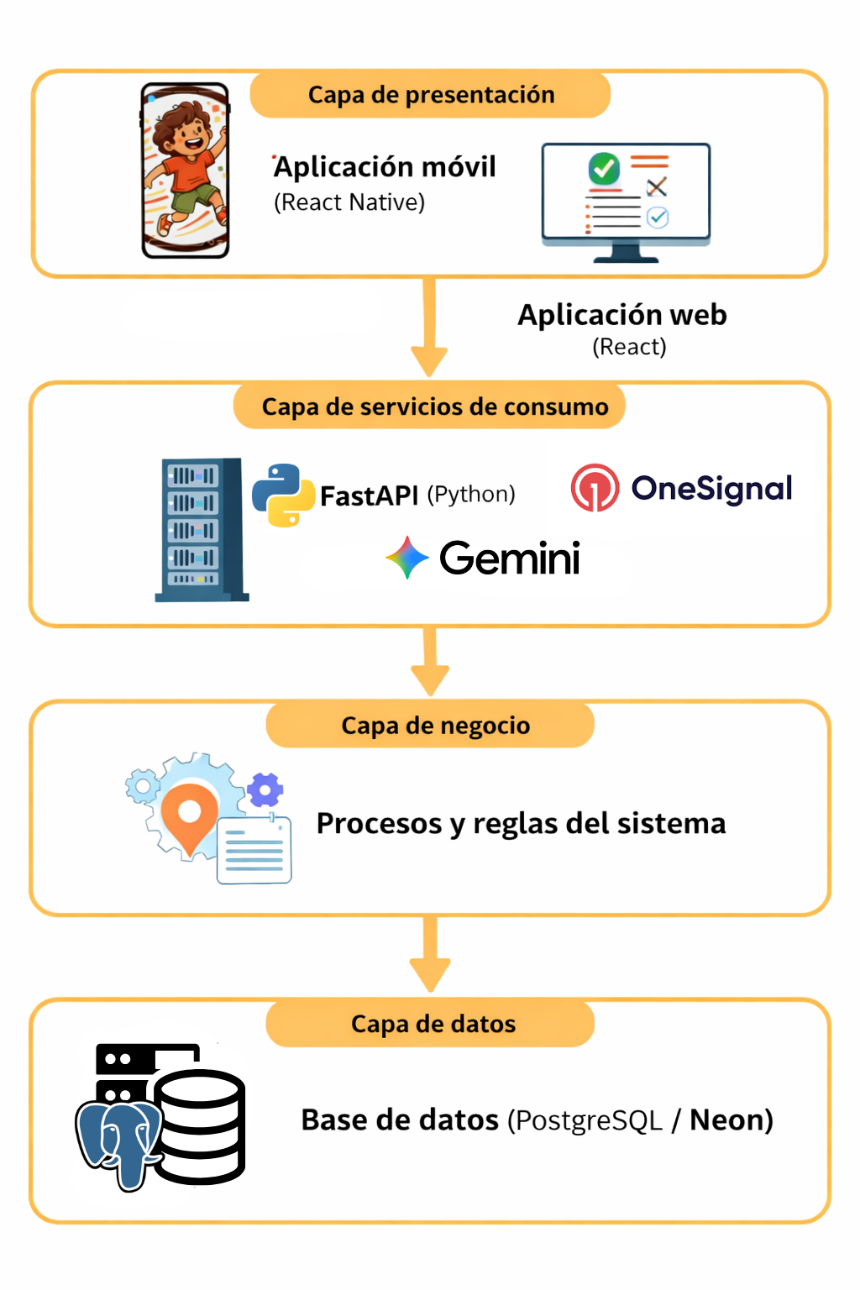
\includegraphics[width=0.75\textwidth]{images/image11.png}
				\end{figure} 
				\tblnote
				
			\subsection{Análisis detallado de requisitos}
				En esta fase, correspondiente a la \textit{detailed requirement analysis} de TDDM4IoTS~\cite{GuerreroUlloa2024}, se precisaron y refinaron los requerimientos identificados en la fase previa, estableciendo criterios técnicos de calidad que orientarían el desarrollo. El análisis se organizó siguiendo la lógica iterativa de la metodología: primero los procesos del backend por su rol central en la lógica del sistema, luego los del módulo web orientado a especialistas y finalmente los de la aplicación móvil diferenciando los contextos de padres y modo niño~\cite{GuerreroUlloa2024,Fowler2002}.
				
				Como resultado de esta fase se elaboraron los casos de uso del sistema, que documentan los actores, el propósito, las precondiciones, postcondiciones y los flujos de interacción de cada funcionalidad. La Figura~\ref{fig:uc} presenta el diagrama de casos de uso principales del sistema FitKids.
				
				\begin{figure}[H]
					\centering
					\caption{Casos de uso principales del sistema FitKids}
					\label{fig:uc}
					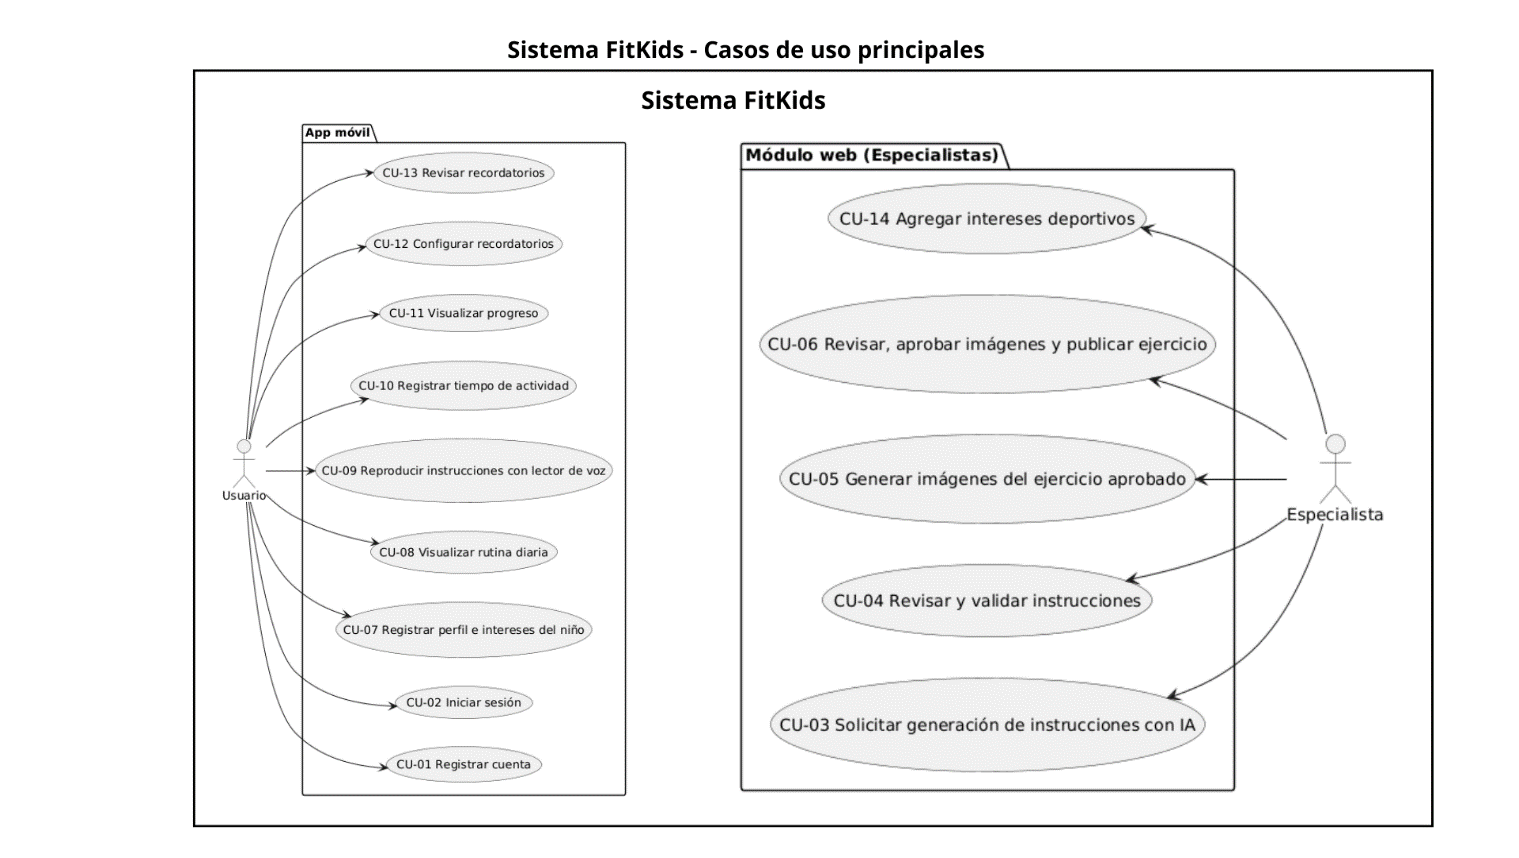
\includegraphics[width=0.95\textwidth]{images/image12.png}
				\end{figure} 
				\tblnote
				
				Como se aprecia en la Figura~\ref{fig:uc}, el sistema organiza su funcionalidad en dos módulos diferenciados por perfil de usuario. El \textbf{módulo de aplicación móvil} agrupa doce casos de uso accesibles al Usuario (que actúa indistintamente como padre o como niño según el modo activo): registro de cuenta (CU-01), inicio de sesión (CU-02), registro del perfil e intereses del niño (CU-07), visualización de rutina diaria (CU-08), reproducción de instrucciones con lector de voz (CU-09), registro del tiempo de actividad (CU-10), visualización del progreso (CU-11), configuración de recordatorios (CU-12) y revisión de recordatorios (CU-13). El \textbf{módulo web para especialistas} concentra los casos de uso de contenido: solicitar la generación de instrucciones con IA (CU-03), revisar y validar las instrucciones generadas (CU-04), generar imágenes del ejercicio aprobado (CU-05), revisar, aprobar imágenes y publicar el ejercicio (CU-06), y agregar intereses deportivos al catálogo del sistema (CU-14). Esta separación operacionaliza el principio de mínimo privilegio~\cite{LOPDP2021}: cada perfil accede únicamente a las funciones que le corresponden, sin posibilidad de interferir en las operaciones de otros actores.
				
				La distribución de casos de uso evidencia la trazabilidad directa entre los requisitos definidos y las funcionalidades implementadas: los nueve requisitos funcionales (RF1--RF9) se mapean unívocamente sobre los catorce casos de uso, siendo RF1 (Generación de rutinas) el que concentra el mayor número de interacciones entre módulos, al depender de que CU-03 a CU-06 hayan sido ejecutados previamente por el especialista para que el contenido esté disponible~\cite{GuerreroUlloa2024,Fowler2002}. Este análisis detallado permitió delimitar el alcance definitivo de cada iteración de desarrollo y establecer las dependencias entre componentes que condicionarían la secuencia de implementación en la fase siguiente.
	
				% ============================================================
				% CASOS DE USO — Sistema FitKids
				% Color encabezado: btnGold RGB(185,130,38) — tono de la app
				% Requiere en preámbulo:
				%   \definecolor{headblue}{RGB}{185,130,38}   % renombrado a tono app
				%   \definecolor{grpgray}{RGB}{232,222,205}   % blobBeige de la app
				%   \usepackage{longtable,colortbl,xcolor,graphicx}
				% ============================================================
				
				% ── Macro compartida ──────────────────────────────────────────
				\newcommand{\cuheader}[2]{%   #1=código  #2=nombre
					\rowcolor{headblue}\multicolumn{2}{c}{\textbf{\color{white}Caso de uso ``#2''}}%
				}
				\newcommand{\cuheadercont}[1]{%  #1=nombre
					\hline\rowcolor{headblue}\multicolumn{2}{c}{\textbf{\color{white}Caso de uso ``#1'' (continuación)}}%
				}
				
				% ════════════════════════════════════════════════════════════
				\begingroup
					\setlength{\LTpre}{6pt}\setlength{\LTpost}{6pt}
					\renewcommand{\arraystretch}{1.20}
					\footnotesize
					\begin{longtable}{p{4cm}p{10.4cm}}
						\caption{Caso de uso ``Registrar cuenta''.}\label{tab:cu01}\\
						\hline
						\rowcolor{headblue}\multicolumn{2}{c}{\textbf{\color{white}Caso de uso ``Registrar cuenta''}}\\\hline
						\endfirsthead
						\hline\rowcolor{headblue}\multicolumn{2}{c}{\textbf{\color{white}Caso de uso ``Registrar cuenta'' (continuación)}}\\\hline
						\endhead
						\hline\multicolumn{2}{r}{\footnotesize\itshape continúa $\rightarrow$}\\
						\endfoot
						\hline\endlastfoot
						\textbf{Código:} CU-01 & \textbf{Actor principal:} Usuario (padre de familia o especialista)\\
						\textbf{Objetivo:} & Permitir que un nuevo usuario cree una cuenta en el sistema FitKids para acceder a sus funcionalidades.\\
						\textbf{Resumen:} & El usuario abre la aplicación, completa el formulario de registro con sus datos personales, acepta los términos y confirma. El sistema valida, crea la cuenta y habilita el acceso.\\
						\textbf{Tipo:} & Principal\\
						\textbf{Requisito asociado:} & RNF4 --- Privacidad y protección de datos\\
						\textbf{Caso de prueba:} & CP-F01\\
						\textbf{Dependencias:} & \textbf{Invoca a:} CU-02. \textbf{Depende de:} Base de datos de usuarios.\\
						\textbf{Precondición:} & No debe haber una sesión de usuario activa en el dispositivo.\\
						\textbf{Postcondición:} & La cuenta queda registrada con contraseña en hash bcrypt; el usuario puede iniciar sesión.\\
						\textbf{Importancia:} & Alta --- Sin registro no es posible acceder a ninguna funcionalidad del sistema.\\\hline
						\multicolumn{2}{c}{\cellcolor{grpgray}\textbf{Flujo normal de eventos}}\\
						\multicolumn{2}{p{14.4cm}}{%
							\begin{tabular}{p{7.0cm}p{7.0cm}}
								\hline
								\centering\textbf{Acción del actor} & \centering\textbf{Respuesta del sistema}\tabularnewline\hline
								1.~Este caso de uso inicia cuando el usuario abre la aplicación sin sesión activa y selecciona ``Crear cuenta''. &\tabularnewline
								& 2.~El sistema presenta el formulario con los campos: nombre, correo, fecha de nacimiento, teléfono, género, dirección y contraseña.\tabularnewline
								3.~El usuario completa todos los campos del formulario. &\tabularnewline
								4.~El usuario acepta los términos y condiciones y presiona ``Registrarse''. &\tabularnewline
								& 5.~El sistema valida campos, formato del correo, coincidencia de contraseñas y unicidad del correo.\tabularnewline
								& 6.~El sistema crea la cuenta, almacena la contraseña en hash bcrypt y muestra confirmación.\tabularnewline
								7.~Este caso de uso finaliza cuando el usuario es redirigido a la pantalla de inicio de sesión (CU-02). &\tabularnewline\hline
							\end{tabular}%
						}\\\hline
						\textbf{Flujo alterno} &
						\textbf{5a. Correo ya registrado:}\newline
						5a.1.~El sistema muestra: ``Este correo ya está en uso. Ingresa uno diferente.''\newline
						5a.2.~El usuario ingresa un correo diferente.\newline
						5a.3.~El flujo vuelve al paso~5.\newline\newline
						\textbf{5b. Contraseñas no coinciden:}\newline
						5b.1.~El sistema resalta el campo de confirmación con el mensaje correspondiente.\newline
						5b.2.~El usuario corrige el campo.\newline
						5b.3.~El flujo vuelve al paso~5.\newline\newline
						\textbf{5c. Campo obligatorio vacío:}\newline
						5c.1.~El sistema resalta el campo e impide continuar.\newline
						5c.2.~El usuario completa el campo faltante.\newline
						5c.3.~El flujo vuelve al paso~5.
						\\\hline
						\textbf{Interfaz de usuario:} & \begin{center}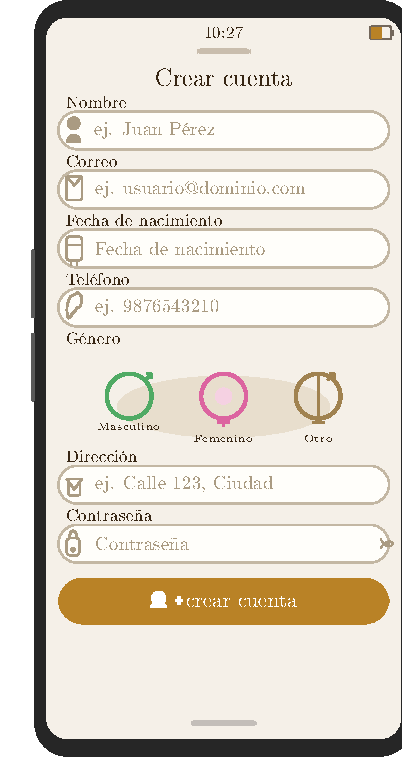
\includegraphics[width=0.40\linewidth,keepaspectratio]{images/cu01_ui.pdf}\end{center}\\\hline
						\textbf{Comentarios:} & Contraseña mínimo 8 caracteres. Correo validado con formato RFC~5322. Los términos deben aceptarse para habilitar el botón.\\\hline
					\end{longtable}
				\endgroup
				\vspace{12pt}
				\tblnote
				\bigskip
				
				% ════════════════════════════════════════════════════════════
				\begingroup
					\setlength{\LTpre}{6pt}\setlength{\LTpost}{6pt}
					\renewcommand{\arraystretch}{1.20}
					\footnotesize
					\begin{longtable}{p{4cm}p{10.4cm}}
						\caption{Caso de uso ``Iniciar sesión''.}\label{tab:cu02}\\
						\hline
						\rowcolor{headblue}\multicolumn{2}{c}{\textbf{\color{white}Caso de uso ``Iniciar sesión''}}\\\hline
						\endfirsthead
						\hline\rowcolor{headblue}\multicolumn{2}{c}{\textbf{\color{white}Caso de uso ``Iniciar sesión'' (continuación)}}\\\hline
						\endhead
						\hline\multicolumn{2}{r}{\footnotesize\itshape continúa $\rightarrow$}\\\endfoot
						\hline\endlastfoot
						\textbf{Código:} CU-02 & \textbf{Actor principal:} Usuario (padre de familia o especialista)\\
						\textbf{Objetivo:} & Autenticar al usuario registrado para acceder al sistema FitKids.\\
						\textbf{Resumen:} & El usuario ingresa su correo y contraseña. El sistema los verifica y otorga acceso al menú principal. Desde la misma pantalla, los niños pueden acceder mediante código (CU-02 bifurca hacia modo niño).\\
						\textbf{Tipo:} & Principal\\
						\textbf{Requisito asociado:} & RNF4 --- Privacidad y protección de datos; RF5 --- Supervisión adulta\\
						\textbf{Caso de prueba:} & CP-F02\\
						\textbf{Dependencias:} & \textbf{Invocado por:} CU-01. \textbf{Invoca a:} CU-07 a CU-13 (perfil adulto), modo niño (CU-08 a CU-10).\\
						\textbf{Precondición:} & No debe haber sesión activa; la cuenta debe existir en el sistema.\\
						\textbf{Postcondición:} & El usuario accede al menú principal correspondiente a su perfil (padre o especialista).\\
						\textbf{Importancia:} & Alta --- Es el punto de entrada a todas las funcionalidades del sistema.\\\hline
						\multicolumn{2}{c}{\cellcolor{grpgray}\textbf{Flujo normal de eventos}}\\\hline
						\multicolumn{2}{p{14.4cm}}{%
							\begin{tabular}{p{7.0cm}p{7.0cm}}
								\hline
								\centering\textbf{Acción del actor} & \centering\textbf{Respuesta del sistema}\tabularnewline\hline
								1.~Este caso de uso inicia cuando el usuario abre la aplicación sin sesión activa. &\tabularnewline
								& 2.~El sistema muestra la pantalla de inicio de sesión con campos de correo y contraseña.\tabularnewline
								3.~El usuario ingresa su correo electrónico y contraseña. &\tabularnewline
								4.~El usuario presiona ``Iniciar sesión''. &\tabularnewline
								& 5.~El sistema verifica las credenciales contra la base de datos.\tabularnewline
								& 6.~El sistema genera un token de sesión y redirige al menú principal del perfil correspondiente.\tabularnewline
								7.~Este caso de uso finaliza cuando el usuario visualiza su menú principal. &\tabularnewline
							\end{tabular}%
						}\\\hline
						\textbf{Flujo alterno} &
						\textbf{5a. Credenciales incorrectas:}\newline
						5a.1.~El sistema muestra: ``Correo o contraseña incorrectos.''\newline
						5a.2.~El usuario corrige los datos.\newline
						5a.3.~El flujo vuelve al paso~5.\newline\newline
						\textbf{1a. El usuario es un niño:}\newline
						1a.1.~El usuario selecciona ``Soy niño --- Ingresar código''.\newline
						1a.2.~El sistema presenta la pantalla de ingreso de código de 6 caracteres.\newline
						1a.3.~Este caso de uso finaliza e inicia el flujo del modo niño (CU-08).
						\\\hline
						\textbf{Interfaz de usuario:} & \begin{center}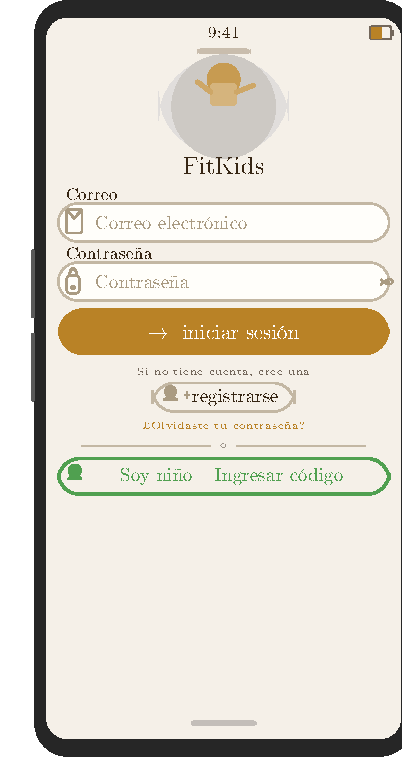
\includegraphics[width=0.40\linewidth,keepaspectratio]{images/cu02_ui.pdf}\end{center}\\\hline
						\textbf{Comentarios:} & El botón ``Soy niño'' está disponible en la misma pantalla. El token de sesión persiste hasta que el usuario cierra sesión manualmente.\\\hline
					\end{longtable}
					\vspace{12pt}
					\tblnote
				\endgroup
				\bigskip
				
				El caso de uso CU-01 (Tabla~\ref{tab:cu01}) y CU-02 (Tabla~\ref{tab:cu02}) constituyen los únicos casos de uso compartidos entre todos los perfiles del sistema: tanto padres como especialistas se registran e inician sesión a través del mismo flujo, lo que unifica la gestión de identidad en un único componente del backend y reduce la superficie de autenticación que debe asegurarse. La bifurcación hacia el modo niño ocurre dentro de CU-02, no como un caso de uso separado de acceso, sino como una ruta alternativa que activa un contexto de menor privilegio con código de un solo uso.
				
				% ════════════════════════════════════════════════════════════
				\begingroup
					\setlength{\LTpre}{6pt}\setlength{\LTpost}{6pt}
					\renewcommand{\arraystretch}{1.20}
					\footnotesize
					\begin{longtable}{p{4cm}p{10.4cm}}
						\caption{Caso de uso ``Solicitar generación de instrucciones con IA''.}\label{tab:cu03}\\
						\hline
						\rowcolor{headblue}\multicolumn{2}{c}{\textbf{\color{white}Caso de uso ``Solicitar generación de instrucciones con IA''}}\\\hline
						\endfirsthead
						\hline\rowcolor{headblue}\multicolumn{2}{c}{\textbf{\color{white}Caso de uso ``Solicitar generación de instrucciones con IA'' (continuación)}}\\\hline
						\endhead
						\hline\multicolumn{2}{r}{\footnotesize\itshape continúa $\rightarrow$}\\\endfoot
						\hline\endlastfoot
						\textbf{Código:} CU-03 & \textbf{Actor principal:} Especialista\\\hline
						\textbf{Objetivo:} & Generar un conjunto de ejercicios físicos mediante inteligencia artificial, segmentados por interés deportivo y rango de edad, para poblar el catálogo del sistema.\\
						\textbf{Resumen:} & El especialista accede al módulo web, selecciona intereses y rango de edad, y solicita la generación. El modelo Gemini produce los ejercicios que quedan en estado ``Pendiente de revisión''.\\
						\textbf{Tipo:} & Principal\\
						\textbf{Requisito asociado:} & RF2 --- Validación de ejercicios por especialistas\\
						\textbf{Caso de prueba:} & CP-F04\\
						\textbf{Dependencias:} & \textbf{Invoca a:} CU-04. \textbf{Depende de:} API Gemini, base de datos de ejercicios, catálogo de intereses (CU-14).\\
						\textbf{Precondición:} & El especialista debe tener sesión iniciada en el módulo web; la API de Gemini debe estar disponible.\\
						\textbf{Postcondición:} & Los ejercicios generados quedan almacenados con estado ``Pendiente de revisión'' en la base de datos.\\
						\textbf{Importancia:} & Alta --- Sin ejercicios generados no es posible poblar el catálogo ni generar rutinas.\\\hline
						\multicolumn{2}{c}{\cellcolor{grpgray}\textbf{Flujo normal de eventos}}\\\hline
						\multicolumn{2}{p{14.4cm}}{%
							\begin{tabular}{p{7.0cm}p{7.0cm}}
								\hline
								\centering\textbf{Acción del actor} & \centering\textbf{Respuesta del sistema}\tabularnewline\hline
								1.~Este caso de uso inicia cuando el especialista accede al módulo web y selecciona ``Generador de Ejercicios''. &\tabularnewline
								& 2.~El sistema presenta el formulario con la lista de intereses deportivos disponibles y los tres rangos de edad (6--7, 8--9, 10--11 años).\tabularnewline
								3.~El especialista selecciona uno o más intereses y el rango de edad objetivo. &\tabularnewline
								4.~El especialista presiona ``Generar Ejercicios''. &\tabularnewline
								& 5.~El sistema construye el prompt con los parámetros seleccionados y envía la solicitud al modelo Gemini.\tabularnewline
								& 6.~El sistema recibe la respuesta, almacena los ejercicios con estado ``Pendiente de revisión'' y redirige al especialista a la pantalla de revisión (CU-04).\tabularnewline
								7.~Este caso de uso finaliza cuando el especialista visualiza el listado de ejercicios pendientes. &\tabularnewline
							\end{tabular}%
						}\\\hline
						\textbf{Flujo alterno} &
						\textbf{5a. La API de Gemini no responde (timeout):}\newline
						5a.1.~El sistema muestra: ``No se pudo generar la rutina con IA. Intenta nuevamente.''\newline
						5a.2.~El especialista reintenta la solicitud.\newline
						5a.3.~El flujo vuelve al paso~5.\newline\newline
						\textbf{3a. Ningún interés seleccionado:}\newline
						3a.1.~El sistema resalta el campo e impide continuar.\newline
						3a.2.~El especialista selecciona al menos un interés.\newline
						3a.3.~El flujo vuelve al paso~4.
						\\\hline
						\textbf{Interfaz de usuario:} & \begin{center}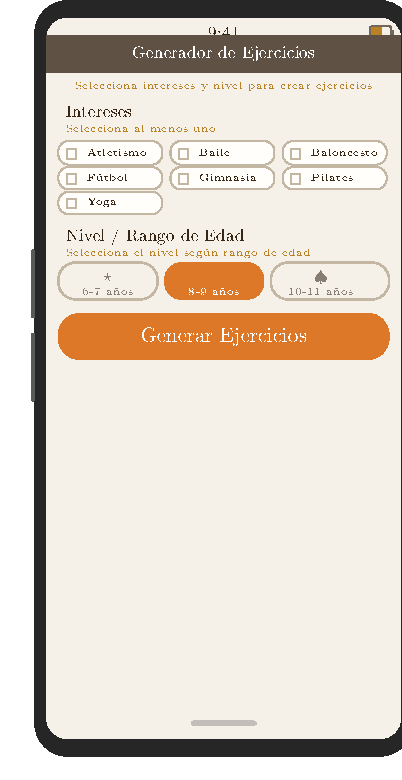
\includegraphics[width=0.40\linewidth,keepaspectratio]{images/cu03_ui.pdf}\end{center}\\\hline
						\textbf{Comentarios:} & El timeout de la llamada a Gemini está configurado en 10~000~ms. Los ejercicios generados incluyen nombre, descripción, pasos y tipo (calentamiento, principal, estiramiento).\\\hline
					\end{longtable}
					\vspace{12pt}
					\tblnote
				\endgroup\bigskip
				
				% ════════════════════════════════════════════════════════════
				\begingroup
					\setlength{\LTpre}{6pt}\setlength{\LTpost}{6pt}
					\renewcommand{\arraystretch}{1.20}
					\footnotesize
					\begin{longtable}{p{4cm}p{10.4cm}}
						\caption{Caso de uso ``Revisar y validar instrucciones''.}\label{tab:cu04}\\
						\hline
						\rowcolor{headblue}\multicolumn{2}{c}{\textbf{\color{white}Caso de uso ``Revisar y validar instrucciones''}}\\\hline
						\endfirsthead
						\hline\rowcolor{headblue}\multicolumn{2}{c}{\textbf{\color{white}Caso de uso ``Revisar y validar instrucciones'' (continuación)}}\\\hline
						\endhead
						\hline\multicolumn{2}{r}{\footnotesize\itshape continúa $\rightarrow$}\\\endfoot
						\hline\endlastfoot
						\textbf{Código:} CU-04 & \textbf{Actor principal:} Especialista\\\hline
						\textbf{Objetivo:} & Garantizar que los ejercicios generados por IA sean clínicamente seguros y apropiados antes de hacerlos disponibles en el sistema.\\
						\textbf{Resumen:} & El especialista revisa cada ejercicio pendiente, analiza nombre, descripción y pasos, y decide aprobarlo o rechazarlo individualmente o en bloque.\\
						\textbf{Tipo:} & Principal\\
						\textbf{Requisito asociado:} & RF2 --- Validación de ejercicios por especialistas; RNF1 --- Seguridad clínica\\
						\textbf{Caso de prueba:} & CP-F05\\
						\textbf{Dependencias:} & \textbf{Invocado por:} CU-03. \textbf{Invoca a:} CU-05 (si aprueba ejercicios).\\
						\textbf{Precondición:} & Deben existir ejercicios en estado ``Pendiente de revisión'' en la base de datos.\\
						\textbf{Postcondición:} & Cada ejercicio revisado cambia a estado ``Aprobado'' o ``Rechazado''; los aprobados quedan disponibles para generación de imágenes.\\
						\textbf{Importancia:} & Alta --- Operacionaliza el modelo \textit{human-in-the-loop} que garantiza la seguridad clínica del contenido.\\\hline
						\multicolumn{2}{c}{\cellcolor{grpgray}\textbf{Flujo normal de eventos}}\\\hline
						\multicolumn{2}{p{14.4cm}}{%
							\begin{tabular}{p{7.0cm}p{7.0cm}}
								\hline
								\centering\textbf{Acción del actor} & \centering\textbf{Respuesta del sistema}\tabularnewline\hline
								1.~Este caso de uso inicia cuando el especialista accede a la pantalla ``Revisión de Ejercicios'' (desde CU-03 o directamente). &\tabularnewline
								& 2.~El sistema presenta las tarjetas de ejercicios pendientes con nombre, categoría, interés, descripción y pasos.\tabularnewline
								3.~El especialista lee el contenido de un ejercicio y presiona ``Aprobar'' o ``Rechazar''. &\tabularnewline
								& 4.~El sistema actualiza el estado del ejercicio en la base de datos y actualiza el contador de aprobados/rechazados.\tabularnewline
								5.~El especialista repite el paso~3 para cada ejercicio pendiente. &\tabularnewline
								6.~Este caso de uso finaliza cuando el especialista presiona ``Generar Imágenes'' para los ejercicios aprobados, iniciando CU-05. &\tabularnewline
							\end{tabular}%
						}\\\hline
						\textbf{Flujo alterno} &
						\textbf{3a. El especialista usa ``Aprobar Todos'':}\newline
						3a.1.~El sistema cambia todos los ejercicios pendientes a estado ``Aprobado'' en una sola operación.\newline
						3a.2.~El flujo continúa en el paso~6.\newline\newline
						\textbf{3b. El especialista usa ``Rechazar Todos'':}\newline
						3b.1.~El sistema cambia todos los ejercicios pendientes a estado ``Rechazado''.\newline
						3b.2.~Este caso de uso finaliza sin invocar CU-05.
						\\\hline
						\textbf{Interfaz de usuario:} & \begin{center}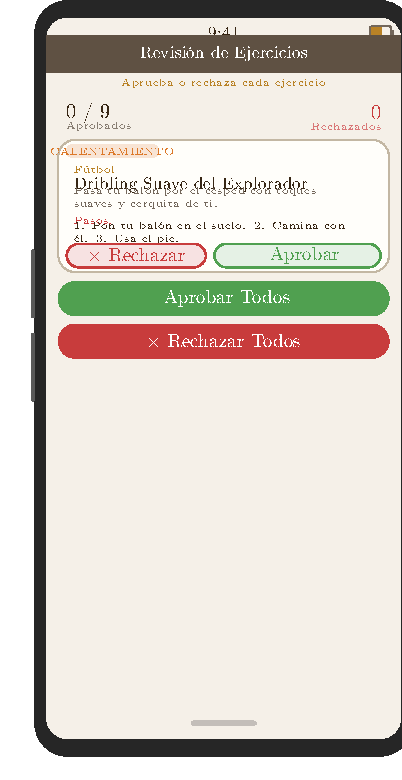
\includegraphics[width=0.40\linewidth,keepaspectratio]{images/cu04_ui.pdf}\end{center}\\\hline
						\textbf{Comentarios:} & El filtro por tipo (calentamiento, principal, estiramiento) facilita la revisión segmentada. El contador muestra en tiempo real cuántos ejercicios han sido aprobados y rechazados.\\\hline
					\end{longtable}
					\vspace{12pt}
					\tblnote
				\endgroup\bigskip
				
				% ════════════════════════════════════════════════════════════
				\begingroup
					\setlength{\LTpre}{6pt}\setlength{\LTpost}{6pt}
					\renewcommand{\arraystretch}{1.20}
					\footnotesize
					\begin{longtable}{p{4cm}p{10.4cm}}
						\caption{Caso de uso ``Generar imágenes del ejercicio aprobado''.}\label{tab:cu05}\\
						\hline
						\rowcolor{headblue}\multicolumn{2}{c}{\textbf{\color{white}Caso de uso ``Generar imágenes del ejercicio aprobado''}}\\\hline
						\endfirsthead
						\hline\rowcolor{headblue}\multicolumn{2}{c}{\textbf{\color{white}Caso de uso ``Generar imágenes del ejercicio aprobado'' (continuación)}}\\\hline
						\endhead
						\hline\multicolumn{2}{r}{\footnotesize\itshape continúa $\rightarrow$}\\\endfoot
						\hline\endlastfoot
						\textbf{Código:} CU-05 & \textbf{Actor principal:} Especialista\\\hline
						\textbf{Objetivo:} & Generar ilustraciones visuales de los ejercicios aprobados para que los niños comprendan la ejecución sin depender exclusivamente del texto.\\
						\textbf{Resumen:} & El especialista solicita la generación de imágenes para los ejercicios aprobados. El sistema llama al modelo Gemini de generación de imagen y asocia el resultado a cada ejercicio.\\
						\textbf{Tipo:} & Principal\\
						\textbf{Requisito asociado:} & RF2 --- Validación de ejercicios por especialistas; RF1 --- Generación de rutinas\\
						\textbf{Caso de prueba:} & CP-F05\\
						\textbf{Dependencias:} & \textbf{Invocado por:} CU-04. \textbf{Invoca a:} CU-06.\\
						\textbf{Precondición:} & Deben existir ejercicios en estado ``Aprobado'' sin imagen asociada; la API de Gemini debe estar disponible.\\
						\textbf{Postcondición:} & Cada ejercicio aprobado tiene una imagen ilustrativa asociada y está listo para publicación.\\
						\textbf{Importancia:} & Alta --- La imagen es el componente visual principal en la interfaz del modo niño.\\\hline
						\multicolumn{2}{c}{\cellcolor{grpgray}\textbf{Flujo normal de eventos}}\\\hline
						\multicolumn{2}{p{14.4cm}}{%
							\begin{tabular}{p{7.0cm}p{7.0cm}}
								\hline
								\centering\textbf{Acción del actor} & \centering\textbf{Respuesta del sistema}\tabularnewline\hline
								1.~Este caso de uso inicia cuando el especialista presiona ``Generar Imágenes para \textit{N} ejercicios'' (desde CU-04). &\tabularnewline
								& 2.~El sistema envía solicitudes de generación de imagen al modelo Gemini para cada ejercicio aprobado, utilizando el nombre y la descripción como prompt.\tabularnewline
								& 3.~El sistema recibe las imágenes, las almacena y las asocia a cada ejercicio en la base de datos.\tabularnewline
								& 4.~El sistema muestra la confirmación: ``¡Imágenes generadas exitosamente!'' con opciones de aprobación masiva.\tabularnewline
								5.~Este caso de uso finaliza cuando el especialista revisa el resultado y procede a CU-06. &\tabularnewline
							\end{tabular}%
						}\\\hline
						\textbf{Flujo alterno} &
						\textbf{3a. Error en generación de imagen para un ejercicio:}\newline
						3a.1.~El sistema marca ese ejercicio con estado de imagen ``Pendiente'' y continúa con los demás.\newline
						3a.2.~El especialista puede reintentar la generación para los ejercicios sin imagen.\newline
						3a.3.~El flujo vuelve al paso~2 para los ejercicios afectados.
						\\\hline
						\textbf{Interfaz de usuario:} & \begin{center}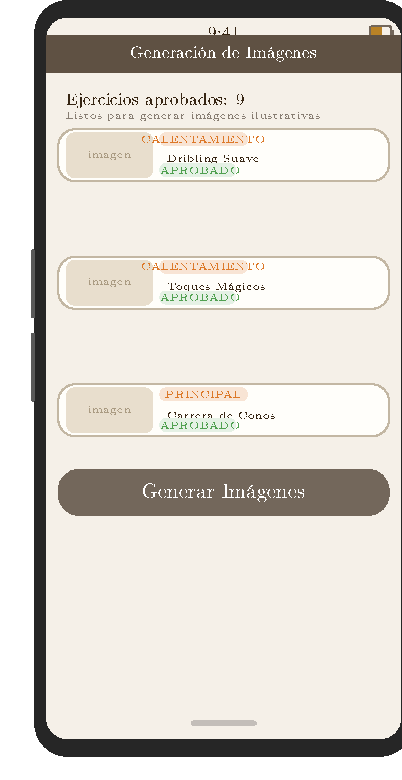
\includegraphics[width=0.40\linewidth,keepaspectratio]{images/cu05_ui.pdf}\end{center}\\\hline
						\textbf{Comentarios:} & Las imágenes generadas son ilustraciones de estilo cómic infantil, coherentes con la estética de la app. El especialista puede aprobar o marcar como pendientes las imágenes antes de publicar.\\\hline
					\end{longtable}
					\vspace{12pt}
					\tblnote
				\endgroup\bigskip
				
				% ════════════════════════════════════════════════════════════
				\begingroup
					\setlength{\LTpre}{6pt}\setlength{\LTpost}{6pt}
					\renewcommand{\arraystretch}{1.20}
					\footnotesize
					\begin{longtable}{p{4cm}p{10.4cm}}
						\caption{Caso de uso ``Revisar, aprobar imágenes y publicar ejercicio''.}\label{tab:cu06}\\
						\hline
						\rowcolor{headblue}\multicolumn{2}{c}{\textbf{\color{white}Caso de uso ``Revisar, aprobar imágenes y publicar ejercicio''}}\\\hline
						\endfirsthead
						\hline\rowcolor{headblue}\multicolumn{2}{c}{\textbf{\color{white}Caso de uso ``Revisar, aprobar imágenes y publicar ejercicio'' (continuación)}}\\\hline
						\endhead
						\hline\multicolumn{2}{r}{\footnotesize\itshape continúa $\rightarrow$}\\\endfoot
						\hline\endlastfoot
						\textbf{Código:} CU-06 & \textbf{Actor principal:} Especialista\\\hline
						\textbf{Objetivo:} & Publicar al catálogo activo los ejercicios que han superado la revisión de instrucciones y cuentan con imágenes aprobadas.\\
						\textbf{Resumen:} & El especialista confirma la aprobación de las imágenes generadas y publica el lote de ejercicios, dejándolos disponibles para que el sistema los incluya en rutinas personalizadas.\\
						\textbf{Tipo:} & Principal\\
						\textbf{Requisito asociado:} & RF1 --- Generación de rutinas validadas por especialistas\\
						\textbf{Caso de prueba:} & CP-F06\\
						\textbf{Dependencias:} & \textbf{Invocado por:} CU-05.\\
						\textbf{Precondición:} & Deben existir ejercicios con imágenes generadas pendientes de publicación.\\
						\textbf{Postcondición:} & Los ejercicios publicados pasan a estado ``Publicado'' y quedan disponibles en el catálogo para la generación de rutinas.\\
						\textbf{Importancia:} & Alta --- Sin ejercicios publicados el sistema no puede generar rutinas para los niños.\\\hline
						\multicolumn{2}{c}{\cellcolor{grpgray}\textbf{Flujo normal de eventos}}\\\hline
						\multicolumn{2}{p{14.4cm}}{%
							\begin{tabular}{p{7.0cm}p{7.0cm}}
								\hline
								\centering\textbf{Acción del actor} & \centering\textbf{Respuesta del sistema}\tabularnewline
								1.~Este caso de uso inicia cuando el sistema muestra la confirmación de imágenes generadas (desde CU-05). &\tabularnewline
								2.~El especialista selecciona ``Aprobar Todas las Imágenes''. &\tabularnewline
								& 3.~El sistema marca todas las imágenes como aprobadas.\tabularnewline
								4.~El especialista presiona ``Publicar \textit{N} Ejercicios con Imágenes''. &\tabularnewline
								& 5.~El sistema cambia el estado de los ejercicios a ``Publicado'' y los hace disponibles en el catálogo activo.\tabularnewline
								6.~Este caso de uso finaliza cuando el sistema confirma la publicación exitosa. &\tabularnewline
							\end{tabular}%
						}\\\hline
						\textbf{Flujo alterno} &
						\textbf{2a. El especialista rechaza algunas imágenes:}\newline
						2a.1.~El especialista selecciona ``Marcar Todas como Pendientes'' para las imágenes no satisfactorias.\newline
						2a.2.~El flujo retorna a CU-05 para regenerar las imágenes rechazadas.\newline
						2a.3.~El flujo vuelve al paso~1 de este caso de uso.
						\\\hline
						\textbf{Interfaz de usuario:} & \begin{center}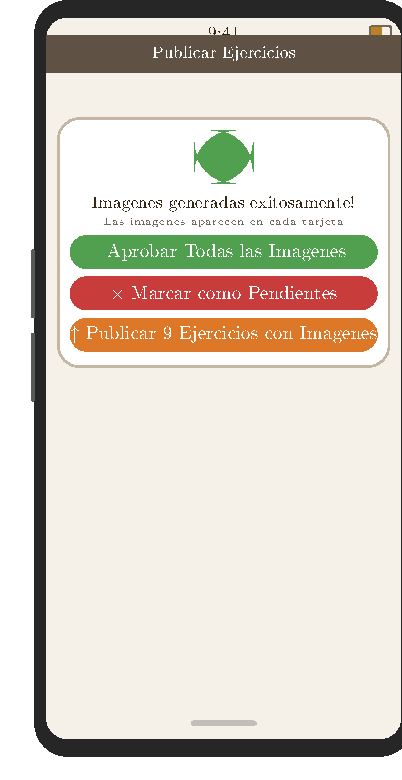
\includegraphics[width=0.40\linewidth,keepaspectratio]{images/cu06_ui.pdf}\end{center}\\\hline
						\textbf{Comentarios:} & La publicación es irreversible desde la interfaz estándar; el estado ``Publicado'' solo puede revertirse desde el panel de administración. Solo los ejercicios publicados participan en la generación de rutinas.\\\hline
					\end{longtable}
					\vspace{12pt}
					\tblnote
				\endgroup\bigskip
				
				Los casos de uso CU-03 a CU-06 (Tablas~\ref{tab:cu03} a~\ref{tab:cu06}) conforman el flujo de validación de contenido del módulo web, cuya ejecución es prerequisito para que el sistema pueda operar en el módulo móvil. Este flujo secuencial ---generación por IA, revisión clínica, generación de imágenes y publicación--- implementa el modelo \textit{human-in-the-loop} identificado como necesario en el análisis preliminar~\cite{Yim2024,Zaleski2026}: ningún ejercicio puede llegar al niño sin haber superado la aprobación explícita del especialista en los pasos CU-04 y CU-06. La tasa de aprobación del 84\% registrada durante la evaluación (sobre 50 ejercicios generados) confirma que el flujo funcionó según lo diseñado y que el 16\% de rechazos justifica la permanencia del filtro humano~\cite{GuerreroUlloa2024}.
				
				% ════════════════════════════════════════════════════════════
				\begingroup
					\setlength{\LTpre}{6pt}\setlength{\LTpost}{6pt}
					\renewcommand{\arraystretch}{1.20}
					\footnotesize
					\begin{longtable}{p{4cm}p{10.4cm}}
						\caption{Caso de uso ``Registrar perfil e intereses del niño''.}\label{tab:cu07}\\
						\hline
						\rowcolor{headblue}\multicolumn{2}{c}{\textbf{\color{white}Caso de uso ``Registrar perfil e intereses del niño''}}\\\hline
						\endfirsthead
						\hline\rowcolor{headblue}\multicolumn{2}{c}{\textbf{\color{white}Caso de uso ``Registrar perfil e intereses del niño'' (continuación)}}\\\hline
						\endhead
						\hline\multicolumn{2}{r}{\footnotesize\itshape continúa $\rightarrow$}\\\endfoot
						\hline\endlastfoot
						\textbf{Código:} CU-07 & \textbf{Actor principal:} Usuario (padre de familia)\\\hline
						\textbf{Objetivo:} & Crear el perfil del niño con sus datos físicos e intereses deportivos, que el sistema utilizará como parámetros para personalizar las rutinas.\\
						\textbf{Resumen:} & El padre completa un formulario de dos pasos: datos básicos (apodo, rango de edad, género, altura, peso, condiciones) y selección de intereses deportivos. El sistema almacena el perfil y lo vincula a la cuenta adulta.\\
						\textbf{Tipo:} & Principal\\
						\textbf{Requisito asociado:} & RF3 --- Adaptación a gustos del niño; RF5 --- Supervisión adulta\\
						\textbf{Caso de prueba:} & CP-F03\\
						\textbf{Dependencias:} & \textbf{Depende de:} CU-02 (sesión activa). \textbf{Invoca a:} CU-08 (el perfil es prerequisito para generar rutinas).\\
						\textbf{Precondición:} & El padre debe tener sesión iniciada en la aplicación móvil.\\
						\textbf{Postcondición:} & El perfil del niño queda almacenado con sus datos físicos e intereses; el sistema puede usarlos como entrada al generador de rutinas.\\
						\textbf{Importancia:} & Alta --- Sin perfil registrado no es posible personalizar rutinas ni generar el código de acceso al modo niño.\\\hline
						\multicolumn{2}{c}{\cellcolor{grpgray}\textbf{Flujo normal de eventos}}\\\hline
						\multicolumn{2}{p{14.4cm}}{%
							\begin{tabular}{p{7.0cm}p{7.0cm}}
								\hline
								\centering\textbf{Acción del actor} & \centering\textbf{Respuesta del sistema}\tabularnewline\hline
								1.~Este caso de uso inicia cuando el padre selecciona ``Agregar niño'' desde el menú principal. &\tabularnewline
								& 2.~El sistema presenta el formulario de paso 1: apodo, rango de edad, género, altura, peso y condiciones médicas opcionales.\tabularnewline
								3.~El padre completa los datos del paso~1 y presiona ``Continuar''. &\tabularnewline
								& 4.~El sistema valida los campos obligatorios y presenta el formulario de paso 2: lista de intereses deportivos disponibles.\tabularnewline
								5.~El padre selecciona los intereses del niño y presiona ``Guardar y finalizar''. &\tabularnewline
								& 6.~El sistema almacena el perfil completo vinculado a la cuenta adulta y muestra confirmación.\tabularnewline
								7.~Este caso de uso finaliza cuando el perfil aparece en la lista de perfiles de la cuenta. &\tabularnewline
							\end{tabular}%
						}\\\hline
						\textbf{Flujo alterno} &
						\textbf{4a. Campo obligatorio vacío en paso~1:}\newline
						4a.1.~El sistema resalta el campo y muestra el mensaje de error correspondiente.\newline
						4a.2.~El padre completa el campo faltante.\newline
						4a.3.~El flujo vuelve al paso~3.\newline\newline
						\textbf{5a. Ningún interés seleccionado:}\newline
						5a.1.~El sistema muestra: ``Selecciona al menos un interés para personalizar la rutina.''\newline
						5a.2.~El padre selecciona al menos un interés.\newline
						5a.3.~El flujo vuelve al paso~5.
						\\\hline
						\textbf{Interfaz de usuario:} & \begin{center}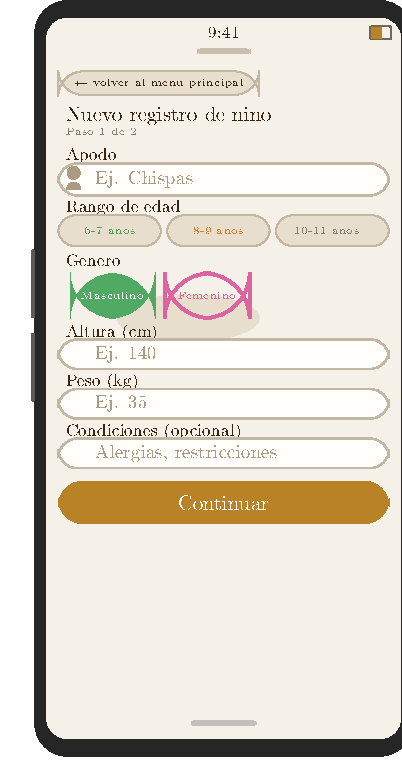
\includegraphics[width=0.40\linewidth,keepaspectratio]{images/cu07_ui.pdf}\end{center}\\\hline
						\textbf{Comentarios:} & Un padre puede registrar múltiples perfiles de niño (1:N). Las condiciones médicas declaradas se incluyen como restricciones en el prompt de generación de rutinas (RNF1).\\\hline
					\end{longtable}
					\vspace{12pt}
					\tblnote
				\endgroup\bigskip
				
				CU-07 (Tabla~\ref{tab:cu07}) es el único caso de uso que conecta directamente los dos módulos del sistema: los intereses seleccionados por el padre en la aplicación móvil son los mismos parámetros que el especialista utilizó en CU-03 para generar el contenido, estableciendo así la trazabilidad funcional entre el perfil del niño y el catálogo de ejercicios. Un perfil sin intereses registrados no puede acceder a CU-08, lo que hace de CU-07 un prerequisito estructural del flujo de rutina.
				
				% ════════════════════════════════════════════════════════════
				\begingroup
					\setlength{\LTpre}{6pt}\setlength{\LTpost}{6pt}
					\renewcommand{\arraystretch}{1.20}
					\footnotesize
					\begin{longtable}{p{4cm}p{10.4cm}}
						\caption{Caso de uso ``Visualizar rutina diaria''.}\label{tab:cu08}\\
						\hline
						\rowcolor{headblue}\multicolumn{2}{c}{\textbf{\color{white}Caso de uso ``Visualizar rutina diaria''}}\\\hline
						\endfirsthead
						\hline\rowcolor{headblue}\multicolumn{2}{c}{\textbf{\color{white}Caso de uso ``Visualizar rutina diaria'' (continuación)}}\\\hline
						\endhead
						\hline\multicolumn{2}{r}{\footnotesize\itshape continúa $\rightarrow$}\\\endfoot
						\hline\endlastfoot
						\textbf{Código:} CU-08 & \textbf{Actor principal:} Usuario (niño, en modo niño)\\\hline
						\textbf{Objetivo:} & Presentar al niño su rutina de ejercicios diaria personalizada, organizada por interés deportivo, para que pueda iniciar la sesión de actividad física.\\
						\textbf{Resumen:} & El niño accede al modo niño mediante código, visualiza la pantalla ``¡Elige tu misión!'', selecciona el interés deportivo del día y el sistema genera y presenta la rutina correspondiente.\\
						\textbf{Tipo:} & Principal\\
						\textbf{Requisito asociado:} & RF1 --- Generación de rutinas; RF3 --- Adaptación a gustos; RF6 --- Rutinas en el hogar\\
						\textbf{Caso de prueba:} & CP-F07\\
						\textbf{Dependencias:} & \textbf{Depende de:} CU-02 (modo niño con código), CU-07 (perfil existente), CU-06 (catálogo con ejercicios publicados). \textbf{Invoca a:} CU-09, CU-10.\\
						\textbf{Precondición:} & El niño debe haber ingresado con código válido; debe existir perfil registrado con intereses y ejercicios publicados en el catálogo.\\
						\textbf{Postcondición:} & El niño visualiza la rutina del día con sus ejercicios organizados en fases (calentamiento, principal, estiramiento).\\
						\textbf{Importancia:} & Alta --- Es el flujo principal de interacción del niño con el sistema.\\\hline
						\multicolumn{2}{c}{\cellcolor{grpgray}\textbf{Flujo normal de eventos}}\\\hline
						\multicolumn{2}{p{14.4cm}}{%
							\begin{tabular}{p{7.0cm}p{7.0cm}}
								\hline
								\centering\textbf{Acción del actor} & \centering\textbf{Respuesta del sistema}\tabularnewline\hline
								1.~Este caso de uso inicia cuando el niño ingresa su código de acceso y presiona ``¡Entrar a jugar!''. &\tabularnewline
								& 2.~El sistema autentica el código y muestra la pantalla de bienvenida con el nombre del niño y su progreso.\tabularnewline
								3.~El niño presiona ``¡JUGAR AHORA!'' o accede a ``¡Elige tu misión!''. &\tabularnewline
								& 4.~El sistema presenta las tarjetas de intereses deportivos disponibles según el perfil del niño.\tabularnewline
								5.~El niño selecciona un interés y presiona ``JUGAR''. &\tabularnewline
								& 6.~El sistema solicita al backend la generación de una rutina personalizada y presenta la pantalla de preparación previa con recomendaciones.\tabularnewline
								7.~El niño presiona ``¡Siguiente!'' para iniciar la rutina. &\tabularnewline
								& 8.~El sistema presenta el primer ejercicio de la fase de calentamiento.\tabularnewline
								9.~Este caso de uso finaliza e inicia CU-09 y CU-10 de forma integrada. &\tabularnewline
							\end{tabular}%
						}\\\hline
						\textbf{Flujo alterno} &
						\textbf{6a. Sin ejercicios publicados para el interés seleccionado:}\newline
						6a.1.~El sistema muestra: ``No hay ejercicios disponibles para esta actividad. Selecciona otra.''\newline
						6a.2.~El niño selecciona otro interés.\newline
						6a.3.~El flujo vuelve al paso~5.\newline\newline
						\textbf{1a. Código inválido o ya utilizado:}\newline
						1a.1.~El sistema muestra: ``Código incorrecto. Pide a tu papá o mamá que genere uno nuevo.''\newline
						1a.2.~Este caso de uso finaliza sin acceso al modo niño.
						\\\hline
						\textbf{Interfaz de usuario:} & \begin{center}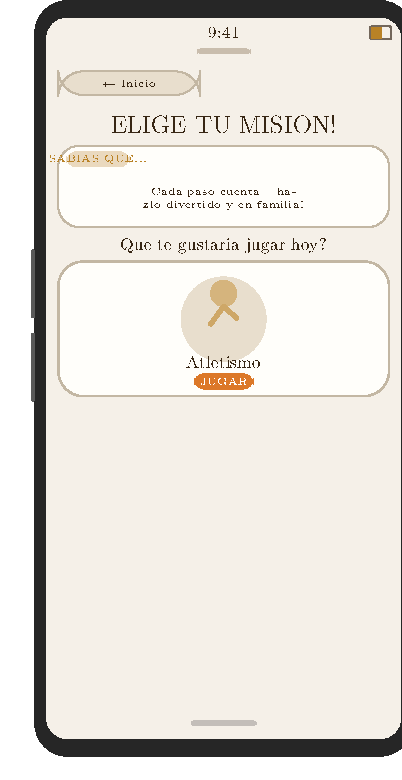
\includegraphics[width=0.40\linewidth,keepaspectratio]{images/cu08_ui.pdf}\end{center}\\\hline
						\textbf{Comentarios:} & El código de acceso es de un solo uso. La rutina generada incluye siempre las tres fases: calentamiento, ejercicios principales y estiramiento. El botón ``¡Quiero otros ejercicios!'' permite regenerar la rutina.\\\hline
					\end{longtable}
					\vspace{12pt}
					\tblnote
				\endgroup\bigskip
				
				% ════════════════════════════════════════════════════════════
				\begingroup
					\setlength{\LTpre}{6pt}\setlength{\LTpost}{6pt}
					\renewcommand{\arraystretch}{1.20}
					\footnotesize
					\begin{longtable}{p{4cm}p{10.4cm}}
						\caption{Caso de uso ``Reproducir instrucciones con lector de voz''.}\label{tab:cu09}\\
						\hline
						\rowcolor{headblue}\multicolumn{2}{c}{\textbf{\color{white}Caso de uso ``Reproducir instrucciones con lector de voz''}}\\\hline
						\endfirsthead
						\hline\rowcolor{headblue}\multicolumn{2}{c}{\textbf{\color{white}Caso de uso ``Reproducir instrucciones con lector de voz'' (continuación)}}\\\hline
						\endhead
						\hline\multicolumn{2}{r}{\footnotesize\itshape continúa $\rightarrow$}\\\endfoot
						\hline\endlastfoot
						\textbf{Código:} CU-09 & \textbf{Actor principal:} Usuario (niño, en modo niño)\\\hline
						\textbf{Objetivo:} & Proporcionar al niño las instrucciones del ejercicio en formato de audio, ampliando la accesibilidad para el rango etario inferior (6--7 años) donde la lectura autónoma no está consolidada.\\
						\textbf{Resumen:} & Durante la ejecución de la rutina, el niño presiona ``Escuchar'' y el sistema sintetiza y reproduce por voz el texto descriptivo del ejercicio activo.\\
						\textbf{Tipo:} & Secundario (complementario a CU-10)\\
						\textbf{Requisito asociado:} & RF9 --- Lector de voz; RNF2 --- Adecuación del lenguaje\\
						\textbf{Caso de prueba:} & CP-F08\\
						\textbf{Dependencias:} & \textbf{Invocado por:} CU-08 (durante la ejecución de la rutina).\\
						\textbf{Precondición:} & El niño debe estar en la pantalla de ejecución de un ejercicio; el dispositivo debe tener audio habilitado.\\
						\textbf{Postcondición:} & El texto del ejercicio activo ha sido reproducido en audio; el niño puede continuar con el ejercicio.\\
						\textbf{Importancia:} & Media --- Amplía la accesibilidad pero no bloquea el flujo principal si no se usa.\\\hline
						\multicolumn{2}{c}{\cellcolor{grpgray}\textbf{Flujo normal de eventos}}\\\hline
						\multicolumn{2}{p{14.4cm}}{%
							\begin{tabular}{p{7.0cm}p{7.0cm}}
								\hline
								\centering\textbf{Acción del actor} & \centering\textbf{Respuesta del sistema}\tabularnewline\hline
								1.~Este caso de uso inicia cuando el niño presiona el botón ``Escuchar'' durante la visualización de un ejercicio. &\tabularnewline
								& 2.~El sistema recupera el texto descriptivo del ejercicio activo.\tabularnewline
								& 3.~El sistema sintetiza el texto mediante el motor de voz configurado y lo reproduce por el altavoz del dispositivo.\tabularnewline
								4.~El niño escucha las instrucciones mientras observa las ilustraciones del ejercicio. &\tabularnewline
								5.~Este caso de uso finaliza cuando la reproducción de audio concluye y el niño continúa con la ejecución del ejercicio. &\tabularnewline
							\end{tabular}%
						}\\\hline
						\textbf{Flujo alterno} &
						\textbf{3a. El dispositivo no tiene audio habilitado:}\newline
						3a.1.~El sistema no reproduce audio.\newline
						3a.2.~Este caso de uso finaliza sin reproducción; el niño puede leer las instrucciones en pantalla.\newline\newline
						\textbf{3b. El texto es demasiado extenso para el motor de voz:}\newline
						3b.1.~El sistema reproduce la primera sección disponible.\newline
						3b.2.~Este caso de uso finaliza con reproducción parcial.
						\\\hline
						\textbf{Interfaz de usuario:} & \begin{center}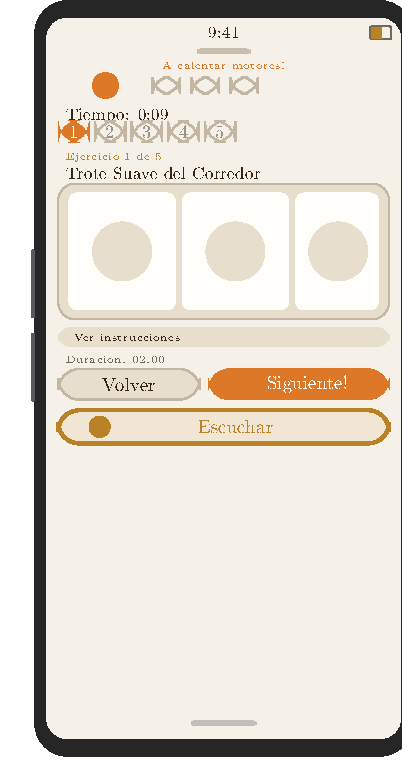
\includegraphics[width=0.40\linewidth,keepaspectratio]{images/cu09_ui.pdf}\end{center}\\\hline
						\textbf{Comentarios:} & La configuración de voz (tipo, volumen y velocidad) es accesible desde la sección de configuración. El botón ``Escuchar'' está disponible en todas las fases de la rutina (calentamiento, principal y estiramiento).\\\hline
					\end{longtable}
					\vspace{12pt}
					\tblnote
				\endgroup\bigskip
				
				% ════════════════════════════════════════════════════════════
				\begingroup
					\setlength{\LTpre}{6pt}\setlength{\LTpost}{6pt}
					\renewcommand{\arraystretch}{1.20}
					\footnotesize
					\begin{longtable}{p{4cm}p{10.4cm}}
						\caption{Caso de uso ``Registrar tiempo de actividad''.}\label{tab:cu10}\\
						\hline
						\rowcolor{headblue}\multicolumn{2}{c}{\textbf{\color{white}Caso de uso ``Registrar tiempo de actividad''}}\\\hline
						\endfirsthead
						\hline\rowcolor{headblue}\multicolumn{2}{c}{\textbf{\color{white}Caso de uso ``Registrar tiempo de actividad'' (continuación)}}\\\hline
						\endhead
						\hline\multicolumn{2}{r}{\footnotesize\itshape continúa $\rightarrow$}\\\endfoot
						\hline\endlastfoot
						\textbf{Código:} CU-10 & \textbf{Actor principal:} Usuario (niño, en modo niño)\\\hline
						\textbf{Objetivo:} & Registrar automáticamente el tiempo de actividad física realizado por el niño durante la sesión, para alimentar el historial de progreso.\\
						\textbf{Resumen:} & Durante la ejecución de la rutina, el sistema cronometra el tiempo activo por ejercicio. Al presionar ``¡Ejercicio completado!'', el tiempo se suma al registro diario del niño.\\
						\textbf{Tipo:} & Principal\\
						\textbf{Requisito asociado:} & RF7 --- Registro del tiempo de actividad\\
						\textbf{Caso de prueba:} & CP-F09\\
						\textbf{Dependencias:} & \textbf{Invocado por:} CU-08. \textbf{Alimenta:} CU-11 (visualización del progreso).\\
						\textbf{Precondición:} & El niño debe estar en la pantalla de ejecución de un ejercicio con la rutina iniciada.\\
						\textbf{Postcondición:} & El tiempo de la sesión queda registrado en la base de datos asociado al perfil del niño y a la fecha; el progreso se actualiza en tiempo real.\\
						\textbf{Importancia:} & Alta --- Es la fuente de datos primaria para los indicadores de progreso y adherencia.\\\hline
						\multicolumn{2}{c}{\cellcolor{grpgray}\textbf{Flujo normal de eventos}}\\\hline
						\multicolumn{2}{p{14.4cm}}{%
							\begin{tabular}{p{7.0cm}p{7.0cm}}
								\hline
								\centering\textbf{Acción del actor} & \centering\textbf{Respuesta del sistema}\tabularnewline\hline
								1.~Este caso de uso inicia cuando el niño comienza la visualización del primer ejercicio de la rutina. &\tabularnewline
								& 2.~El sistema inicia el temporizador visible en pantalla y comienza el conteo del tiempo activo.\tabularnewline
								3.~El niño realiza el ejercicio y presiona ``¡Ejercicio completado!''. &\tabularnewline
								& 4.~El sistema detiene el temporizador para ese ejercicio, marca el indicador visual como completado y acumula el tiempo al total de la sesión.\tabularnewline
								5.~El niño repite el paso~3 para cada ejercicio de la rutina. &\tabularnewline
								& 6.~Al completar todos los ejercicios, el sistema muestra la pantalla de felicitación con el tiempo total acumulado y almacena el registro en la base de datos.\tabularnewline
								7.~Este caso de uso finaliza cuando el registro queda persistido y el progreso es visible en el historial (CU-11). &\tabularnewline
							\end{tabular}%
						}\\\hline
						\textbf{Flujo alterno} &
						\textbf{3a. El niño abandona la rutina antes de completarla:}\newline
						3a.1.~El niño presiona ``Volver'' o cierra la aplicación.\newline
						3a.2.~El sistema registra el tiempo parcial acumulado hasta ese momento con estado ``Incompleta''.\newline
						3a.3.~Este caso de uso finaliza con registro parcial.
						\\\hline
						\textbf{Interfaz de usuario:} & \begin{center}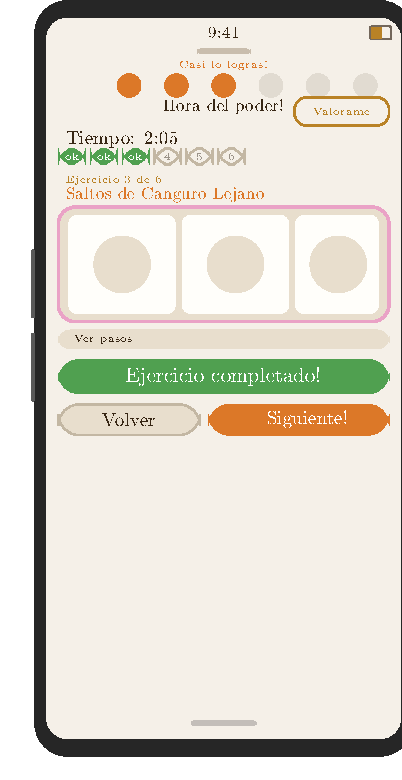
\includegraphics[width=0.40\linewidth,keepaspectratio]{images/cu10_ui.pdf}\end{center}\\\hline
						\textbf{Comentarios:} & El temporizador es visible durante toda la ejecución. El registro persiste en la base de datos en menos de 5 segundos tras finalizar la sesión. El tiempo acumulado incluye todas las fases: calentamiento, ejercicios principales y estiramiento.\\\hline
					\end{longtable}
					\vspace{12pt}
					\tblnote
				\endgroup\bigskip
				
				Los casos de uso CU-08 a CU-10 (Tablas~\ref{tab:cu08} a~\ref{tab:cu10}) conforman el núcleo de interacción del modo niño y se ejecutan de forma integrada durante cada sesión de actividad. CU-08 es el punto de entrada y decisión ---selección de misión---, CU-09 es opcional y no bloquea el flujo principal, y CU-10 opera en segundo plano registrando el tiempo de forma automática a medida que el niño avanza por los ejercicios. Esta arquitectura de flujo minimiza las decisiones que el niño debe tomar durante la sesión, principio de diseño especialmente relevante para el rango etario inferior (6--7 años) donde la carga cognitiva debe ser mínima~\cite{Hourcade2015}.
				
				% ════════════════════════════════════════════════════════════
				\begingroup
					\setlength{\LTpre}{6pt}\setlength{\LTpost}{6pt}
					\renewcommand{\arraystretch}{1.20}
					\footnotesize
					\begin{longtable}{p{4cm}p{10.4cm}}
						\caption{Caso de uso ``Visualizar progreso''.}\label{tab:cu11}\\
						\hline
						\rowcolor{headblue}\multicolumn{2}{c}{\textbf{\color{white}Caso de uso ``Visualizar progreso''}}\\\hline
						\endfirsthead
						\hline\rowcolor{headblue}\multicolumn{2}{c}{\textbf{\color{white}Caso de uso ``Visualizar progreso'' (continuación)}}\\\hline
						\endhead
						\hline\multicolumn{2}{r}{\footnotesize\itshape continúa $\rightarrow$}\\\endfoot
						\hline\endlastfoot
						\textbf{Código:} CU-11 & \textbf{Actor principal:} Usuario (padre de familia)\\\hline
						\textbf{Objetivo:} & Permitir al padre consultar el historial de actividad física del niño, incluyendo días completados, tiempo acumulado y comparativa semanal.\\
						\textbf{Resumen:} & El padre accede a la pantalla de progreso, selecciona el período de consulta y el sistema presenta un gráfico de barras semanal con el historial detallado por día.\\
						\textbf{Tipo:} & Principal\\
						\textbf{Requisito asociado:} & RF8 --- Visualización del progreso\\
						\textbf{Caso de prueba:} & CP-F10\\
						\textbf{Dependencias:} & \textbf{Alimentado por:} CU-10. \textbf{Depende de:} Base de datos de registros de actividad.\\
						\textbf{Precondición:} & El padre debe tener sesión iniciada; deben existir registros de actividad previos del niño.\\
						\textbf{Postcondición:} & El padre ha consultado el historial; el sistema queda en espera de nueva interacción.\\
						\textbf{Importancia:} & Alta --- Provee al padre la retroalimentación necesaria para monitorear la adherencia del niño.\\\hline
						\multicolumn{2}{c}{\cellcolor{grpgray}\textbf{Flujo normal de eventos}}\\\hline
						\multicolumn{2}{p{14.4cm}}{%
							\begin{tabular}{p{7.0cm}p{7.0cm}}
								\hline
								\centering\textbf{Acción del actor} & \centering\textbf{Respuesta del sistema}\tabularnewline\hline
								1.~Este caso de uso inicia cuando el padre selecciona ``Ver progreso'' desde el perfil del niño. &\tabularnewline
								& 2.~El sistema consulta los registros de actividad del niño y presenta el gráfico de barras semanal con el período en curso.\tabularnewline
								3.~El padre selecciona un período diferente para comparar semanas anteriores. &\tabularnewline
								& 4.~El sistema actualiza el gráfico con los datos del período seleccionado.\tabularnewline
								5.~El padre expande ``Detalle e Historial'' para ver el registro día a día. &\tabularnewline
								& 6.~El sistema muestra cada fecha con el estado (Completada/No realizada) y los minutos activos registrados.\tabularnewline
								7.~Este caso de uso finaliza cuando el padre navega fuera de la pantalla de progreso. &\tabularnewline
							\end{tabular}%
						}\\\hline
						\textbf{Flujo alterno} &
						\textbf{2a. Sin registros de actividad para el período seleccionado:}\newline
						2a.1.~El sistema muestra el gráfico vacío con el mensaje: ``Sin actividad registrada en este período.''\newline
						2a.2.~El padre puede seleccionar otro período o cerrar la pantalla.\newline
						2a.3.~El flujo vuelve al paso~3.
						\\\hline
						\textbf{Interfaz de usuario:} & \begin{center}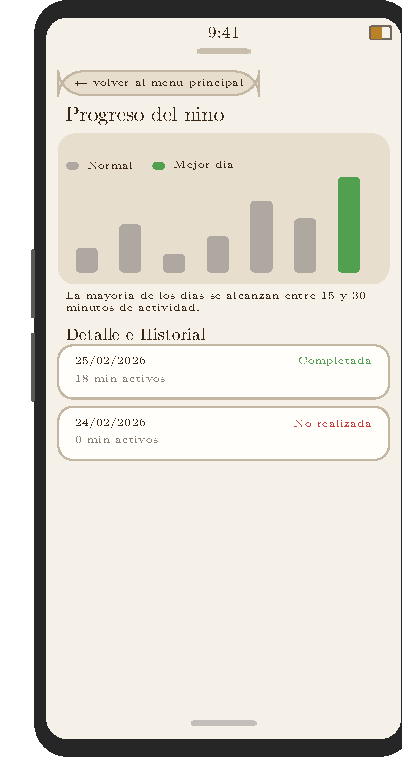
\includegraphics[width=0.40\linewidth,keepaspectratio]{images/cu11_ui.pdf}\end{center}\\\hline
						\textbf{Comentarios:} & El gráfico distingue visualmente el ``mejor día'' (mayor tiempo activo) con color diferenciado. El análisis textual generado por el sistema resume el patrón de actividad de la semana.\\\hline
					\end{longtable}
					\vspace{12pt}
					\tblnote
				\endgroup\bigskip
				
				% ════════════════════════════════════════════════════════════
				\begingroup
					\setlength{\LTpre}{6pt}\setlength{\LTpost}{6pt}
					\renewcommand{\arraystretch}{1.20}
					\footnotesize
					\begin{longtable}{p{4cm}p{10.4cm}}
						\caption{Caso de uso ``Configurar recordatorios''.}\label{tab:cu12}\\
						\hline
						\rowcolor{headblue}\multicolumn{2}{c}{\textbf{\color{white}Caso de uso ``Configurar recordatorios''}}\\\hline
						\endfirsthead
						\hline\rowcolor{headblue}\multicolumn{2}{c}{\textbf{\color{white}Caso de uso ``Configurar recordatorios'' (continuación)}}\\\hline
						\endhead
						\hline\multicolumn{2}{r}{\footnotesize\itshape continúa $\rightarrow$}\\\endfoot
						\hline\endlastfoot
						\textbf{Código:} CU-12 & \textbf{Actor principal:} Usuario (padre de familia)\\\hline
						\textbf{Objetivo:} & Programar notificaciones push que recuerden al niño realizar su rutina de actividad física en los días y horas establecidos por el padre.\\
						\textbf{Resumen:} & El padre activa los recordatorios, selecciona los días de la semana, elige entre uno o dos recordatorios diarios y establece la hora. El sistema guarda la configuración y activa el servicio de notificaciones.\\
						\textbf{Tipo:} & Principal\\
						\textbf{Requisito asociado:} & RF4 --- Recordatorios de actividad física; RF5 --- Supervisión adulta\\
						\textbf{Caso de prueba:} & CP-F11\\
						\textbf{Dependencias:} & \textbf{Depende de:} CU-07 (perfil del niño existente). \textbf{Invoca a:} CU-13 (entrega de la notificación).\\
						\textbf{Precondición:} & El padre debe tener sesión activa; el dispositivo debe tener permisos de notificación push habilitados.\\
						\textbf{Postcondición:} & La configuración queda almacenada y el servicio de notificaciones (OneSignal) activa el recordatorio en el horario programado.\\
						\textbf{Importancia:} & Alta --- Los recordatorios son el mecanismo principal para sostener la adherencia a la rutina en el contexto doméstico.\\\hline
						\multicolumn{2}{c}{\cellcolor{grpgray}\textbf{Flujo normal de eventos}}\\\hline
						\multicolumn{2}{p{14.4cm}}{%
							\begin{tabular}{p{7.0cm}p{7.0cm}}
								\hline
								\centering\textbf{Acción del actor} & \centering\textbf{Respuesta del sistema}\tabularnewline\hline
								1.~Este caso de uso inicia cuando el padre selecciona ``Configurar recordatorios'' desde el perfil del niño. &\tabularnewline
								& 2.~El sistema presenta la pantalla de configuración con el interruptor ON/OFF, el selector de días y la opción de cantidad de recordatorios.\tabularnewline
								3.~El padre activa el interruptor de recordatorios. &\tabularnewline
								4.~El padre selecciona los días de la semana en que el niño realizará ejercicio. &\tabularnewline
								5.~El padre elige la cantidad de recordatorios (1 o 2 al día) y establece la hora. &\tabularnewline
								6.~El padre presiona ``Guardar configuración''. &\tabularnewline
								& 7.~El sistema almacena la configuración, la envía al servicio OneSignal y muestra confirmación de guardado.\tabularnewline
								8.~Este caso de uso finaliza cuando el padre visualiza el mensaje de confirmación. &\tabularnewline
							\end{tabular}%
						}\\\hline
						\textbf{Flujo alterno} &
						\textbf{7a. Error al comunicar con OneSignal:}\newline
						7a.1.~El sistema almacena la configuración localmente y muestra: ``Configuración guardada. El recordatorio se activará cuando se recupere la conexión.''\newline
						7a.2.~Este caso de uso finaliza con configuración guardada en espera de sincronización.\newline\newline
						\textbf{3a. El dispositivo no tiene permisos de notificación:}\newline
						3a.1.~El sistema muestra un mensaje solicitando al padre habilitar los permisos en la configuración del dispositivo.\newline
						3a.2.~El flujo vuelve al paso~3 una vez habilitados los permisos.
						\\\hline
						\textbf{Interfaz de usuario:} & \begin{center}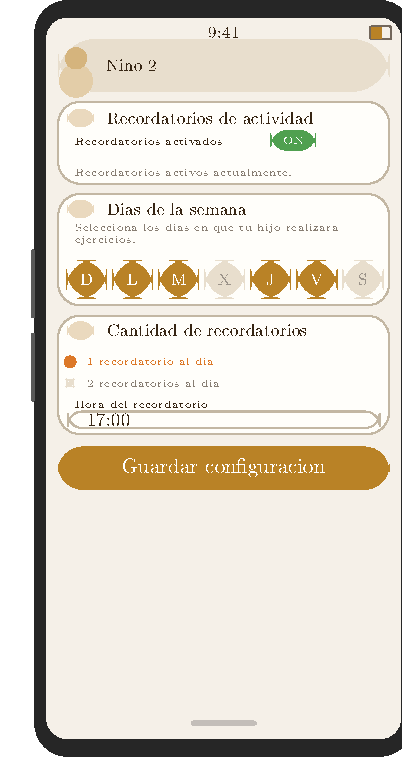
\includegraphics[width=0.40\linewidth,keepaspectratio]{images/cu12_ui.pdf}\end{center}\\\hline
						\textbf{Comentarios:} & La configuración es independiente por perfil de niño. El padre puede desactivar los recordatorios en cualquier momento con el interruptor ON/OFF. La notificación se entrega en un margen de $\pm$1 minuto respecto a la hora configurada.\\\hline
					\end{longtable}
					\vspace{12pt}
					\tblnote
				\endgroup\bigskip
				
				% ════════════════════════════════════════════════════════════
				\begingroup
					\setlength{\LTpre}{6pt}\setlength{\LTpost}{6pt}
					\renewcommand{\arraystretch}{1.20}
					\footnotesize
					\begin{longtable}{p{4cm}p{10.4cm}}
						\caption{Caso de uso ``Revisar recordatorios''.}\label{tab:cu13}\\
						\hline
						\rowcolor{headblue}\multicolumn{2}{c}{\textbf{\color{white}Caso de uso ``Revisar recordatorios''}}\\\hline
						\endfirsthead
						\hline\rowcolor{headblue}\multicolumn{2}{c}{\textbf{\color{white}Caso de uso ``Revisar recordatorios'' (continuación)}}\\\hline
						\endhead
						\hline\multicolumn{2}{r}{\footnotesize\itshape continúa $\rightarrow$}\\\endfoot
						\hline\endlastfoot
						\textbf{Código:} CU-13 & \textbf{Actor principal:} Usuario (padre o niño)\\\hline
						\textbf{Objetivo:} & Recibir la notificación push del recordatorio y acceder a la rutina del día directamente desde ella.\\
						\textbf{Resumen:} & En la hora programada, el sistema envía una notificación push al dispositivo. El usuario toca la notificación y la aplicación lo redirige directamente al flujo de rutina (CU-08).\\
						\textbf{Tipo:} & Secundario (desencadenado por el sistema)\\
						\textbf{Requisito asociado:} & RF4 --- Recordatorios de actividad física\\
						\textbf{Caso de prueba:} & CP-F12\\
						\textbf{Dependencias:} & \textbf{Invocado por:} CU-12 (configuración de recordatorio). \textbf{Invoca a:} CU-08 (si el usuario toca la notificación).\\
						\textbf{Precondición:} & Un recordatorio debe estar configurado y activo; el dispositivo debe tener notificaciones habilitadas.\\
						\textbf{Postcondición:} & El usuario ha sido notificado; si tocó la notificación, se encuentra en la pantalla de rutina del día.\\
						\textbf{Importancia:} & Alta --- Es el mecanismo de activación externo del hábito; sin él la adherencia depende exclusivamente de la iniciativa del usuario.\\\hline
						\multicolumn{2}{c}{\cellcolor{grpgray}\textbf{Flujo normal de eventos}}\\\hline
						\multicolumn{2}{p{14.4cm}}{%
							\begin{tabular}{p{7.0cm}p{7.0cm}}
								\hline
								\centering\textbf{Acción del actor} & \centering\textbf{Respuesta del sistema}\tabularnewline\hline
								1.~Este caso de uso inicia cuando el sistema detecta que se ha alcanzado la hora configurada para el recordatorio. &\tabularnewline
								& 2.~El sistema envía la notificación push a través de OneSignal con el mensaje: ``¡Es hora de ejercitarse! Haz clic para ver tu rutina de hoy.'' al dispositivo registrado.\tabularnewline
								3.~El usuario recibe la notificación en el dispositivo (con la app en cualquier estado). &\tabularnewline
								4.~El usuario toca la notificación. &\tabularnewline
								& 5.~El sistema abre la aplicación y redirige directamente a la pantalla de selección de misión (CU-08).\tabularnewline
								6.~Este caso de uso finaliza cuando el usuario visualiza la pantalla de rutina del día. &\tabularnewline
							\end{tabular}%
						}\\\hline
						\textbf{Flujo alterno} &
						\textbf{4a. El usuario ignora la notificación:}\newline
						4a.1.~El sistema no ejecuta ninguna acción adicional.\newline
						4a.2.~Este caso de uso finaliza sin redireccionamiento.\newline\newline
						\textbf{2a. El dispositivo no tiene conexión en el momento del envío:}\newline
						2a.1.~OneSignal reintenta la entrega cuando el dispositivo recupere conectividad.\newline
						2a.2.~El flujo continúa desde el paso~3 al restaurarse la conexión.
						\\\hline
						\textbf{Interfaz de usuario:} & \begin{center}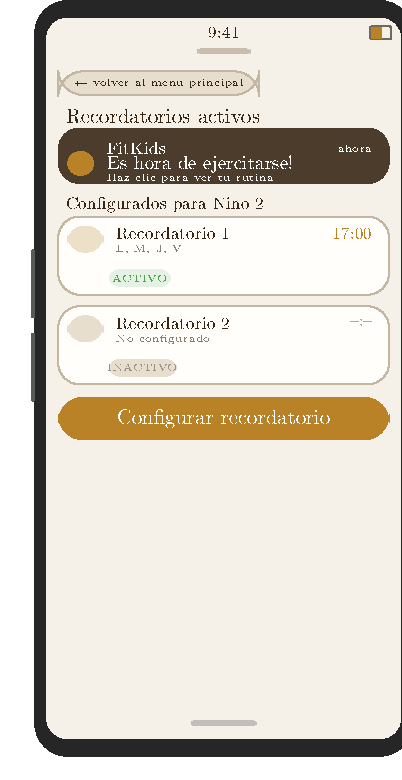
\includegraphics[width=0.40\linewidth,keepaspectratio]{images/cu13_ui.pdf}\end{center}\\\hline
						\textbf{Comentarios:} & La notificación se muestra aunque la app esté cerrada. El texto del recordatorio es fijo y no personalizable desde la interfaz estándar. Los recordatorios se envían solo en los días configurados en CU-12.\\\hline
					\end{longtable}
					\vspace{12pt}
					\tblnote
				\endgroup\bigskip
				
				Los casos de uso CU-11 a CU-13 (Tablas~\ref{tab:cu11} a~\ref{tab:cu13}) son exclusivos del perfil adulto y forman el subsistema de supervisión y adherencia. CU-11 cierra el ciclo conductual al convertir el tiempo registrado por CU-10 en retroalimentación visual consultable por el padre; CU-12 y CU-13 actúan como mecanismo de activación externo del hábito mediante notificaciones push, atendiendo la barrera de adherencia identificada en el análisis de campo~\cite{Schoeppe2017,VegaDiaz2023}. La separación entre configurar (CU-12) y recibir (CU-13) refleja que la notificación es disparada por el sistema de forma autónoma, no por una acción directa del usuario.
				
				% ════════════════════════════════════════════════════════════
				\begingroup
					\setlength{\LTpre}{6pt}\setlength{\LTpost}{6pt}
					\renewcommand{\arraystretch}{1.20}
					\footnotesize
					\begin{longtable}{p{4cm}p{10.4cm}}
						\caption{Caso de uso ``Agregar intereses deportivos''.}\label{tab:cu14}\\
						\hline
						\rowcolor{headblue}\multicolumn{2}{c}{\textbf{\color{white}Caso de uso ``Agregar intereses deportivos''}}\\\hline
						\endfirsthead
						\hline\rowcolor{headblue}\multicolumn{2}{c}{\textbf{\color{white}Caso de uso ``Agregar intereses deportivos'' (continuación)}}\\\hline
						\endhead
						\hline\multicolumn{2}{r}{\footnotesize\itshape continúa $\rightarrow$}\\\endfoot
						\hline\endlastfoot
						\textbf{Código:} CU-14 & \textbf{Actor principal:} Especialista\\\hline
						\textbf{Objetivo:} & Administrar el catálogo de intereses deportivos disponibles en el sistema, agregando, editando o desactivando opciones que los padres pueden asignar al perfil del niño.\\
						\textbf{Resumen:} & El especialista accede al módulo de gestión de intereses, consulta el catálogo actual y puede agregar un nuevo interés o modificar el estado de los existentes (activo/inactivo).\\
						\textbf{Tipo:} & Soporte\\
						\textbf{Requisito asociado:} & RF3 --- Adaptación a gustos del niño\\
						\textbf{Caso de prueba:} & ---\\
						\textbf{Dependencias:} & \textbf{Consultado por:} CU-03 (selección de intereses para generación), CU-07 (selección de intereses del niño).\\
						\textbf{Precondición:} & El especialista debe tener sesión iniciada en el módulo web.\\
						\textbf{Postcondición:} & El catálogo de intereses queda actualizado; los cambios se reflejan inmediatamente en los formularios de generación de ejercicios y de registro de perfil del niño.\\
						\textbf{Importancia:} & Media --- Permite la evolución del catálogo sin intervención técnica, pero el sistema es funcional con el catálogo inicial de 7 intereses.\\\hline
						\multicolumn{2}{c}{\cellcolor{grpgray}\textbf{Flujo normal de eventos}}\\\hline
						\multicolumn{2}{p{14.4cm}}{%
							\begin{tabular}{p{7.0cm}p{7.0cm}}
								\hline
								\centering\textbf{Acción del actor} & \centering\textbf{Respuesta del sistema}\tabularnewline\hline
								1.~Este caso de uso inicia cuando el especialista accede a ``Gestión de Intereses'' desde el menú del módulo web. &\tabularnewline
								& 2.~El sistema presenta el catálogo con los indicadores de total, activos e inactivos, y la lista de intereses con su estado.\tabularnewline
								3.~El especialista presiona ``+ Nuevo interés''. &\tabularnewline
								& 4.~El sistema muestra el formulario de creación con los campos: nombre del interés e ícono representativo.\tabularnewline
								5.~El especialista completa el formulario y confirma. &\tabularnewline
								& 6.~El sistema valida que el nombre no esté duplicado y almacena el nuevo interés con estado ``Activo''.\tabularnewline
								7.~Este caso de uso finaliza cuando el nuevo interés aparece en la lista del catálogo. &\tabularnewline
							\end{tabular}%
						}\\\hline
						\textbf{Flujo alterno} &
						\textbf{6a. El nombre del interés ya existe en el catálogo:}\newline
						6a.1.~El sistema muestra: ``Este interés ya existe. Ingresa un nombre diferente.''\newline
						6a.2.~El especialista modifica el nombre.\newline
						6a.3.~El flujo vuelve al paso~5.\newline\newline
						\textbf{3b. El especialista desactiva un interés existente:}\newline
						3b.1.~El especialista presiona el botón de desactivar junto al interés.\newline
						3b.2.~El sistema cambia su estado a ``Inactivo'' y lo oculta de los formularios de selección.\newline
						3b.3.~Este caso de uso finaliza con el catálogo actualizado.
						\\\hline
						\textbf{Interfaz de usuario:} & \begin{center}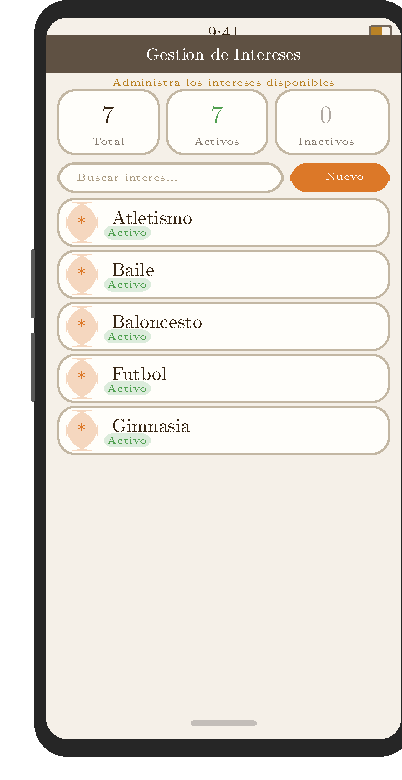
\includegraphics[width=0.40\linewidth,keepaspectratio]{images/cu14_ui.pdf}\end{center}\\\hline
						\textbf{Comentarios:} & Desactivar un interés no elimina los perfiles de niño que lo tienen asignado; solo lo oculta para nuevas asignaciones. El catálogo inicial incluye 7 intereses: Atletismo, Baile, Baloncesto, Fútbol, Gimnasia, Pilates y Yoga.\\\hline
					\end{longtable}
					\vspace{12pt}
					\tblnote
				\endgroup\bigskip
				
				CU-14 (Tabla~\ref{tab:cu14}) es el único caso de uso de soporte del sistema: no forma parte del flujo de actividad física del niño, pero condiciona la variedad del catálogo disponible para CU-03 y CU-07. Su importancia media refleja que el sistema es funcional con el catálogo inicial de siete intereses, pero su presencia en el diseño previene la necesidad de intervención técnica para ampliar la oferta deportiva, atributo de mantenibilidad operativa valorado en la evaluación cualitativa del módulo web por los especialistas participantes.
			
			\subsection{Generación y adaptación de modelos}
			\label{sec:genadapmodel}
				En esta fase, denominada \textit{model generation and adaptation} por TDDM4IoTS~\cite{GuerreroUlloa2024}, se construyeron los modelos formales del sistema con un propósito que va más allá de la documentación: conforme a los principios de la ingeniería dirigida por modelos incorporados en la metodología, el modelado permite abstraer la heterogeneidad tecnológica del sistema, establecer una base conceptual coherente antes de la generación de código y facilitar la comunicación entre el equipo de desarrollo y los actores involucrados~\cite{GuerreroUlloa2024,Fowler2002}. Se elaboraron cuatro modelos UML complementarios que cubren las dimensiones funcional, estructural, de despliegue y de organización modular del sistema, en orden progresivo desde la lógica central del backend hacia las interfaces web y móvil.
				
				El diagrama de casos de uso (Figura~\ref{fig:uc-gen-adap}) evidenció la organización funcional del sistema en tres niveles de interacción, estructurados por el principio de mínimo privilegio~\cite{LOPDP2021}. El nivel correspondiente al especialista concentra las operaciones de mayor impacto sobre el catálogo de contenido: generación, revisión y publicación de ejercicios. El nivel del padre agrupa las funciones de configuración y supervisión: registro del perfil del niño, gestión de recordatorios y consulta del progreso. El nivel del niño es intencionalmente acotado: ejecutar rutinas, registrar actividad física y escuchar instrucciones. Esta jerarquía es la representación directa de RF5 (Supervisión adulta) y RNF4 (Privacidad y protección de datos), que impiden que un perfil acceda a las operaciones de otro.
				
				\begin{figure}[H]
					\centering
					\caption{Casos de uso principales del sistema FitKids}
					\label{fig:uc-gen-adap}
					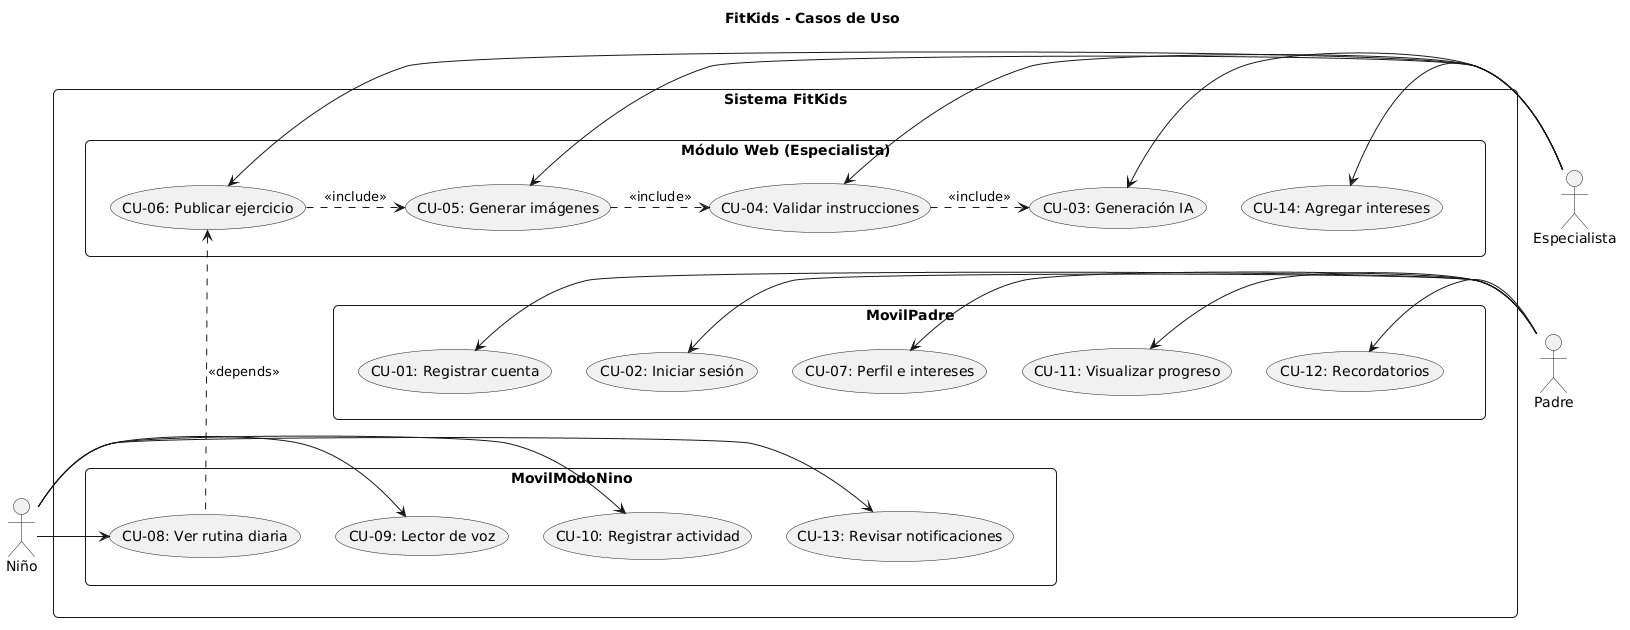
\includegraphics[width=0.9\textwidth]{images/image20.png}
				\end{figure}
				\tblnote
				
				El diagrama de clases (Figura~\ref{fig:class}) estructuró las entidades principales del sistema agrupadas en tres módulos: Módulo Móvil Padre, Módulo Web y Módulo Móvil modo niño. Las cardinalidades clave son: un \texttt{User} puede tener múltiples perfiles de \texttt{Child} (1:N); un \texttt{Child} puede tener múltiples \texttt{Routine} asignadas en fechas distintas (1:N); un \texttt{Exercise} puede aparecer en múltiples \texttt{Routine} y una \texttt{Routine} puede incluir múltiples \texttt{Exercise} (N:M, resuelta mediante la entidad intermedia \texttt{RoutineExercise}); y un \texttt{Child} puede acumular múltiples registros de \texttt{Progress} (1:N), cada uno detallado a nivel de ejercicio mediante \texttt{ProgressExercise}. La clase \texttt{MedicalCondition}, asociada al perfil del niño, encapsula las condiciones clínicas declaradas por el padre y actúa como restricción en el prompt de generación, garantizando que el modelo Gemini respete las limitaciones individuales de cada perfil~\cite{Fowler2002}. La clase \texttt{AIGeneration} registra cada llamada al servicio de inteligencia artificial con su prompt, parámetros y respuesta, lo que habilita la trazabilidad y auditoría del contenido generado, aspecto directamente relacionado con RNF4~\cite{LOPDP2021}. Conforme a lo previsto por TDDM4IoTS, este diagrama sirvió como base para el diseño del esquema relacional de PostgreSQL, estableciendo la trazabilidad directa entre el modelo conceptual y la capa de persistencia~\cite{GuerreroUlloa2024}.
				
				\begin{figure}[H]
					\centering
					\caption{Diagrama de clases del sistema FitKids}
					\label{fig:class}
					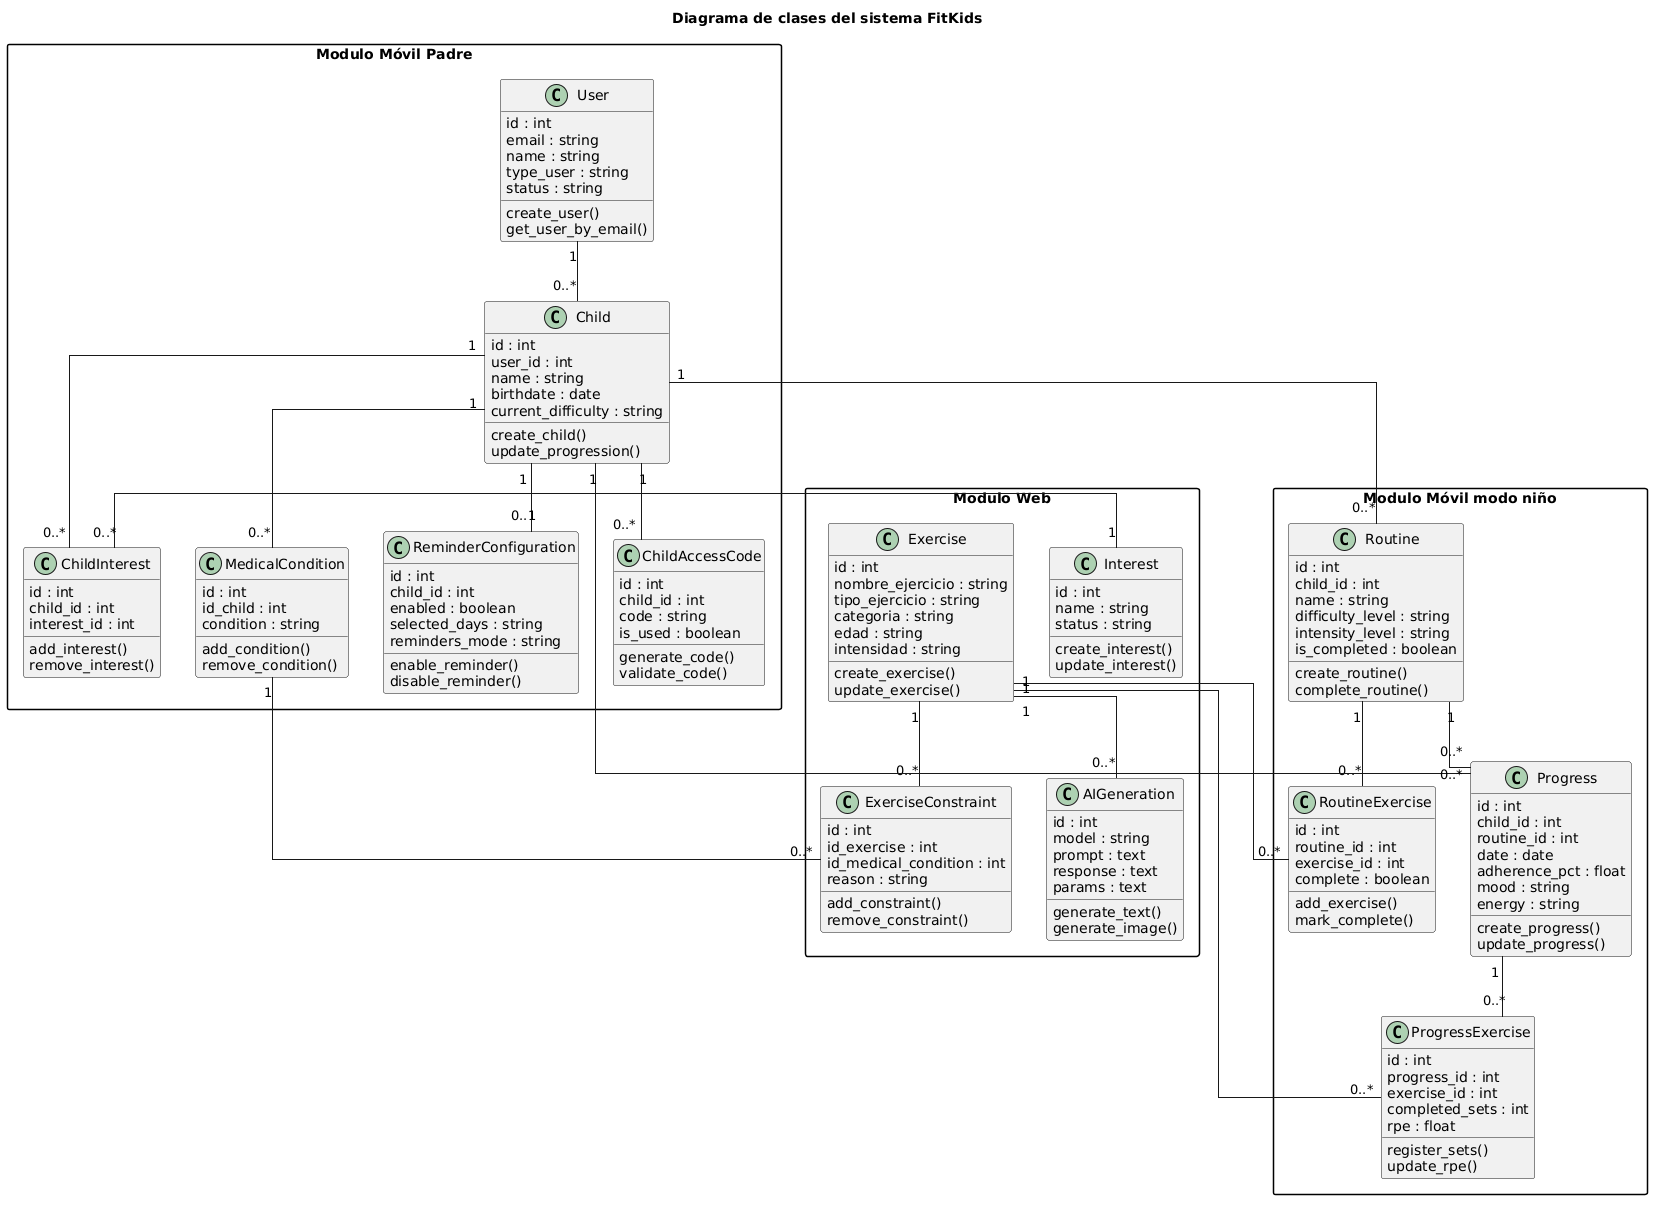
\includegraphics[width=0.9\textwidth]{images/image13.png}
				\end{figure}
				\tblnote
				
				El diagrama de componentes (Figura~\ref{fig:comp}) describe la organización modular del backend, identificando cuatro módulos de lógica independientes dentro de la capa de negocio: Autenticación, Rutinas y Progreso, Catálogo de Ejercicios, y Recordatorios~\cite{Fowler2002}. Todos ellos se comunican con los clientes a través de un componente \textit{API Gateway / Router} centralizado, lo que permite gestionar el enrutamiento, la validación de tokens y el control de acceso en un único punto antes de delegar la solicitud al módulo correspondiente. El módulo de Catálogo de Ejercicios es el único que se comunica con el servicio externo de IA (Google Gemini) mediante una interfaz requerida, mientras que el módulo de Recordatorios se comunica con OneSignal mediante una interfaz requerida separada para la entrega de notificaciones push. Esta separación de interfaces externas por módulo funcional aplica el patrón de adaptador~\cite{Fowler2002}, que permite reemplazar cualquiera de los servicios externos ---por ejemplo, migrar de Gemini a un modelo alternativo--- sin modificar la lógica de los demás módulos, reforzando el atributo de mantenibilidad del sistema~\cite{GuerreroUlloa2024}.
				
				\begin{figure}[H]
					\centering
					\caption{Diagrama de componentes del sistema FitKids}
					\label{fig:comp}
					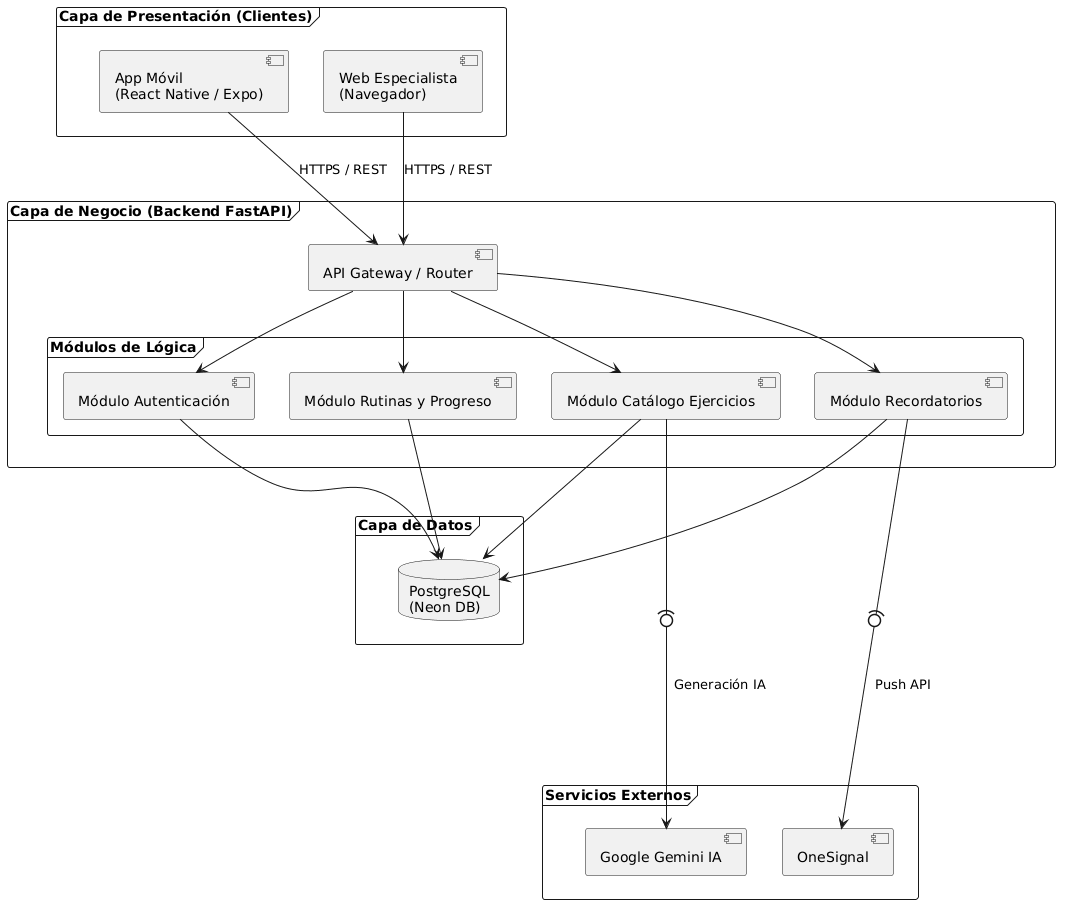
\includegraphics[width=0.9\textwidth]{images/image15.png}
				\end{figure}
				\tblnote
				
				El diagrama de despliegue (Figura~\ref{fig:deploy}) confirma que el sistema opera bajo una arquitectura distribuida con dos tipos de clientes: el dispositivo móvil Android (App FitKids en React Native) y el navegador web del especialista. El flujo de comunicación sigue el camino: clientes $\rightarrow$ API REST en Render (HTTPS, puerto 443) $\rightarrow$ lógica de negocio FastAPI $\rightarrow$ base de datos PostgreSQL en Neon (protocolo Postgres, puerto 5432). Las llamadas al modelo Gemini y al servicio OneSignal se realizan desde el backend como cliente externo (HTTPS, puerto 443), de modo que ningún dato de usuario se transmite directamente desde el dispositivo móvil hacia servicios de terceros~\cite{LOPDP2021,GDPR2016}. Esta decisión arquitectónica, coherente con el principio de minimización de datos, centraliza el procesamiento de información sensible en el backend controlado y elimina la superficie de exposición desde el cliente~\cite{Kleppmann2017}.
				
				\begin{figure}[H]
					\centering
					\caption{Diagrama de despliegue del sistema FitKids}
					\label{fig:deploy}
					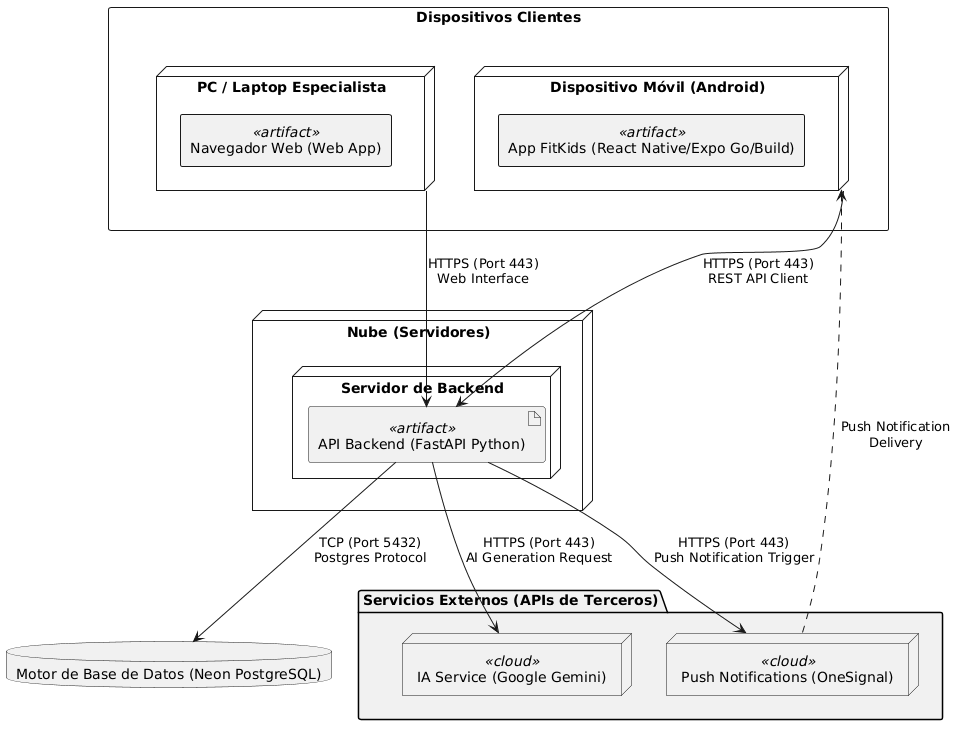
\includegraphics[width=0.9\textwidth]{images/image14.png}
				\end{figure}
				\tblnote
				
				La generación de estos cuatro modelos permitió validar conceptualmente el diseño antes de iniciar la generación de código, identificar inconsistencias entre capas y asegurar la coherencia entre los requisitos definidos, la arquitectura de cuatro capas establecida en la fase anterior y la solución implementada en las fases subsiguientes~\cite{GuerreroUlloa2024,Fowler2002}.

			\subsection{Generación de pruebas}
			\label{sec:gentest}
				En esta fase, correspondiente a la \textit{test generation} de TDDM4IoTS~\cite{GuerreroUlloa2024}, se diseñaron las pruebas que el software debía superar antes de considerarse completado, siguiendo el ciclo rojo-verde-refactorizar propio del desarrollo guiado por pruebas~\cite{GuerreroUlloa2024,Fowler2002}. Las pruebas se organizaron en dos grupos: unitarias, orientadas a verificar el comportamiento aislado de cada módulo; y de integración, orientadas a comprobar la correcta comunicación entre componentes. La definición siguió una lógica progresiva alineada con las iteraciones de la metodología: primero las verificaciones sobre la lógica del backend mediante Pytest, luego los escenarios del módulo web con Vitest y React Testing Library, y finalmente los de la aplicación móvil con Jest y React Native Testing Library, diferenciando los contextos de padres y modo niño~\cite{GuerreroUlloa2024,Fowler2002}.
				
				En el backend se ejecutaron 19 casos de prueba unitaria distribuidos en cuatro módulos: \textit{Child Service} (lógica de progresión y actividad del niño), \textit{Exercise Service} (calificación y promedios de ejercicios), \textit{Progress Service} (cálculo de estadísticas) y \textit{Security} y \textit{User Controller} (autenticación, hashing de contraseñas y gestión de cuentas). Estos módulos concentran la lógica de negocio crítica del sistema, por lo que su verificación unitaria es condición necesaria antes de proceder a las pruebas de integración~\cite{Fowler2002}. Todos los casos fueron superados satisfactoriamente, como se detalla en la Tabla~\ref{tab:pruebas_backend}.
				
				\begingroup
					\setlength{\LTpre}{6pt}\setlength{\LTpost}{2pt}
					\renewcommand{\arraystretch}{1.15}
					\small
					\begin{longtable}{p{2.7cm}p{4.5cm}p{5.2cm}p{1.8cm}}
						\caption{Resultados de pruebas unitarias del backend}\label{tab:pruebas_backend}\\
						\hline
						\textbf{Módulo} & \textbf{Descripción de la prueba} & \textbf{Función de prueba} & \textbf{Resultado}\\
						\hline
						\endfirsthead
						\hline
						\textbf{Módulo} & \textbf{Descripción de la prueba} & \textbf{Función de prueba} & \textbf{Resultado}\\
						\hline
						\endhead
						\hline\multicolumn{4}{r}{\footnotesize\itshape continúa $\rightarrow$}\\
						\endfoot
						\hline
						\endlastfoot
						Child Service & Obtención de actividad dentro de un rango válido & \fn{test\_activity\_from\_range} & Pasó\\
						Child Service & Actualización de nivel de progresión a nivel medio & \fn{test\_update\_progression\_level\_up\_to\_medio} & Pasó\\
						Child Service & Actualización de nivel de progresión a nivel avanzado & \fn{test\_update\_progression\_level\_up\_to\_avanzado} & Pasó\\
						Child Service & Validación de progresión sin cambio de nivel & \fn{test\_update\_progression\_no\_level\_up} & Pasó\\
						Exercise Service & Validación de calificación inválida & \fn{test\_rate\_exercise\_invalid\_rating} & Pasó\\
						Exercise Service & Registro de primera calificación & \fn{test\_rate\_exercise\_first\_rating} & Pasó\\
						Exercise Service & Cálculo del promedio de calificaciones & \fn{test\_rate\_exercise\_average\_calculation} & Pasó\\
						Progress Service & Obtención de estadísticas sin registros & \fn{test\_get\_progress\_statistics\_empty} & Pasó\\
						Progress Service & Cálculo de estadísticas de progreso & \fn{test\_get\_progress\_statistics\_calculation} & Pasó\\
						Security & Generación de hash de contraseña & \fn{test\_hash\_password\_generates\_valid\_hash} & Pasó\\
						Security & Verificación correcta de contraseña & \fn{test\_verify\_password\_success} & Pasó\\
						Security & Verificación incorrecta de contraseña & \fn{test\_verify\_password\_failure} & Pasó\\
						Security & Generación de token de acceso & \fn{test\_create\_access\_token} & Pasó\\
						User Controller & Registro de usuario exitoso & \fn{test\_registrar\_usuario\_exito} & Pasó\\
						User Controller & Registro con correo duplicado & \fn{test\_registrar\_usuario\_email\_duplicado} & Pasó\\
						User Controller & Inicio de sesión exitoso & \fn{test\_login\_usuario\_exito} & Pasó\\
						User Controller & Inicio de sesión con tipo incorrecto & \fn{test\_login\_usuario\_tipo\_incorrecto} & Pasó\\
						User Controller & Inicio de sesión web exitoso & \fn{test\_login\_usuario\_web\_exito} & Pasó\\
						User Controller & Cambio de contraseña incorrecta & \fn{test\_cambiar\_password\_actual\_incorrecta} & Pasó\\
					\end{longtable}
				\endgroup
				
				\vspace{12pt}
				\tblnote
				
				En el módulo web se ejecutaron 7 pruebas unitarias mediante Vitest y React Testing Library, enfocadas en los componentes de autenticación y registro, que son los únicos con lógica de validación de formulario y comunicación con la API propia de este módulo~\cite{Fowler2002}. Todos los casos fueron aprobados sin errores, como se muestra en la Tabla~\ref{tab:pruebas_web}.
				
				\begin{table}[H]
					\centering\small
					\caption{Resultados de pruebas unitarias del módulo web}
					\label{tab:pruebas_web}
					\begin{tabular}{p{3cm}p{8cm}p{2.5cm}}
						\hline
						\textbf{Componente} & \textbf{Funcionalidad evaluada} & \textbf{Resultado}\\
						\hline
						Login & Renderización del formulario de autenticación & Pasó\\
						Login & Manejo de error ante fallo de API & Pasó\\
						Login & Redirección tras autenticación exitosa & Pasó\\
						Register & Renderización del formulario de registro & Pasó\\
						Register & Validación de campos obligatorios & Pasó\\
						Register & Validación de formato de teléfono & Pasó\\
						Register & Construcción correcta del JSON hacia la API & Pasó\\
						\hline
					\end{tabular}
				\end{table}
				\tblnote
				
				En la aplicación móvil para padres se ejecutaron 6 pruebas mediante Jest y React Native Testing Library, orientadas a los flujos de autenticación, validación de formularios y almacenamiento local de la sesión. Estos escenarios cubren las funcionalidades de mayor riesgo de fallo en el contexto de un dispositivo móvil: la persistencia del token de sesión y el manejo de errores de red~\cite{Fowler2002}. Todos los casos resultaron exitosos, como se observa en la Tabla~\ref{tab:pruebas_movil_padres}.
				
				\begin{table}[H]
					\centering\small
					\caption{Resultados de pruebas unitarias del módulo móvil (perfil padres)}
					\label{tab:pruebas_movil_padres}
					\begin{tabular}{p{3cm}p{8cm}p{2.5cm}}
						\hline
						\textbf{Pantalla} & \textbf{Caso de prueba} & \textbf{Resultado}\\
						\hline
						Login & Renderización de componentes de inicio de sesión & Pasó\\
						Login & Manejo de errores de conexión & Pasó\\
						Login & Almacenamiento seguro de sesión & Pasó\\
						Register & Procesamiento del formulario & Pasó\\
						Register & Validación de campos requeridos & Pasó\\
						Register & Envío exitoso de datos al servidor & Pasó\\
						\hline
					\end{tabular}
				\end{table}
				\tblnote
				
				En la aplicación móvil para niños se ejecutaron 6 pruebas que verifican la navegación entre pantallas, la visualización de ejercicios, la interacción con la interfaz y el registro de la actividad realizada. Estos escenarios son los más sensibles desde la perspectiva del usuario final, dado que cualquier fallo en la pantalla de ejecución de ejercicios interrumpiría directamente la sesión de actividad física del niño~\cite{Hourcade2015}. Todos los casos fueron superados sin fallos, como se detalla en la Tabla~\ref{tab:pruebas_movil_ninos}.
				
				\begin{table}[H]
					\centering\small
					\caption{Resultados de pruebas unitarias del módulo móvil (modo niño)}
					\label{tab:pruebas_movil_ninos}
					\begin{tabular}{p{3cm}p{8cm}p{2.5cm}}
						\hline
						\textbf{Pantalla} & \textbf{Funcionalidad evaluada} & \textbf{Resultado}\\
						\hline
						Inicio & Acceso del usuario infantil mediante código & Pasó\\
						Ejercicios & Visualización de actividades de la rutina & Pasó\\
						Ejecución & Interacción con ejercicios físicos & Pasó\\
						Progreso & Registro de actividad realizada & Pasó\\
						Navegación & Fluidez entre pantallas del modo niño & Pasó\\
						Interfaz & Correcta visualización gráfica & Pasó\\
						\hline
					\end{tabular}
				\end{table}
				\tblnote
				
				Las Tablas~\ref{tab:pruebas_backend} a~\ref{tab:pruebas_movil_ninos} confirman que los 38 casos de prueba unitaria ejecutados ---19 en backend, 7 en módulo web, 6 en móvil para padres y 6 en modo niño--- fueron superados en su totalidad, sin fallos detectados. Esta cobertura abarca los cuatro módulos funcionales del sistema y verifica tanto la lógica de negocio crítica como los flujos de interacción de mayor riesgo desde la perspectiva del usuario~\cite{GuerreroUlloa2024,Fowler2002}. Posteriormente se ejecutaron las pruebas de integración para verificar la comunicación entre componentes mediante Pytest con TestClient de FastAPI en el backend y herramientas de testing para la simulación de flujos completos en las interfaces web y móvil. Los resultados se presentan en la Tabla~\ref{tab:pruebas_integracion}.
				
				\begin{table}[H]
					\centering\small
					\caption{Pruebas de integración del sistema}
					\label{tab:pruebas_integracion}
					\begin{tabular}{p{1.8cm}p{2cm}p{3.5cm}p{3cm}p{2.5cm}p{1.5cm}}
						\hline
						\textbf{Código} & \textbf{Módulo} & \textbf{Componentes integrados} & \textbf{Acción de prueba} & \textbf{Resultado esperado} & \textbf{Estado}\\
						\hline
						CP-INT01 & Backend & Backend + Base de datos & Registrar perfil del niño y consultar datos & Datos almacenados y recuperados correctamente & Pasó\\
						CP-INT02 & Web & App web + Backend + IA & Generar instrucciones desde la web & Instrucciones generadas y almacenadas en la BD & Pasó\\
						CP-INT03 & Móvil padres & App móvil + OneSignal & Configurar recordatorio y verificar notificación & Notificación recibida en el horario definido & Pasó\\
						CP-INT04 & Móvil niños & App móvil + Backend & Generar rutina desde modo niño & Rutina personalizada recuperada del servidor & Pasó\\
						CP-INT05 & Móvil niños & App móvil + Base de datos & Registrar tiempo de actividad y consultar progreso & Progreso actualizado correctamente & Pasó\\
						CP-INT06 & Flujo completo & Especialista $\rightarrow$ publicación $\rightarrow$ app móvil & Publicar ejercicio y generar rutina en móvil & Ejercicio publicado disponible para rutina & Pasó\\
						\hline
					\end{tabular}
				\end{table}
				\tblnote

			\subsection{Generación de software}
				\label{sec:sofgen}
				En esta fase, correspondiente a la \textit{software generation} de TDDM4IoTS~\cite{GuerreroUlloa2024}, se materializó la solución a partir de los modelos, requisitos y pruebas definidos en las fases previas, siguiendo el principio del ciclo TDD: el código se escribe para que las pruebas pasen, no a la inversa~\cite{GuerreroUlloa2024,Fowler2002}. El proceso se organizó de forma iterativa, iniciando con la lógica del backend como base de integración y extendiéndose progresivamente hacia el módulo web y la aplicación móvil.
				
				En el backend se implementó el mecanismo de generación de rutinas personalizadas mediante IA. Como se aprecia en la Figura~\ref{fig:gen}, el prompt se construye dinámicamente incorporando variables del perfil del niño: género, edad, altura, peso, interés deportivo y nivel de impacto. El prompt incluye una instrucción crítica de seguridad que evalúa cada ejercicio contra las condiciones médicas del niño (\texttt{lista\_condiciones\_nino}) y obliga al modelo a incluir las contraindicaciones en la respuesta JSON estructurada~\cite{LOPDP2021,GuerreroUlloa2024}. La respuesta es parseada directamente desde el campo \texttt{text} de la respuesta de Gemini, lo que hace que la validación del esquema sea responsabilidad del prompt y no del código receptor.
				
				\begin{figure}[H]
					\centering
					\caption{Construcción dinámica del prompt para generación de rutinas con Gemini}
					\label{fig:gen}
					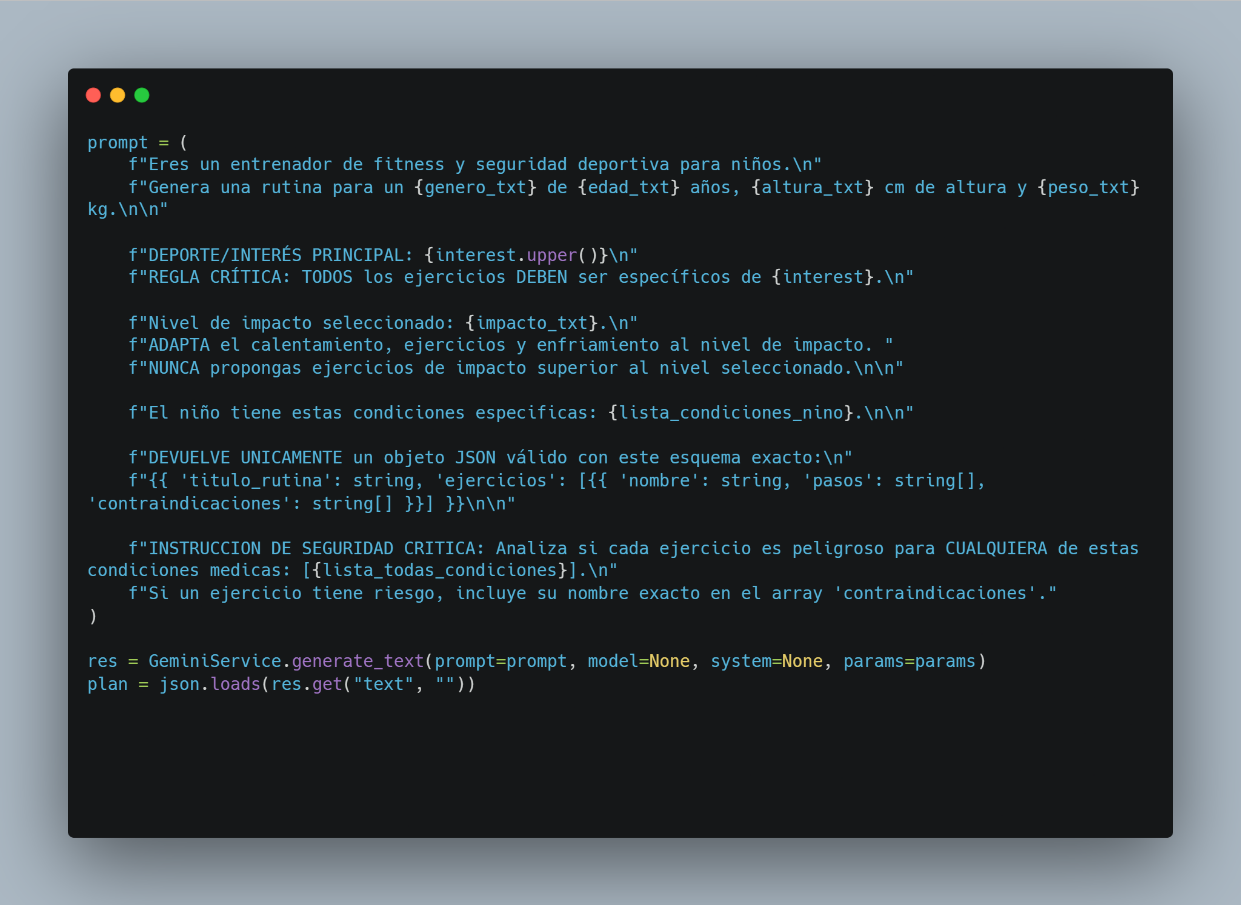
\includegraphics[width=0.9\textwidth]{images/image16.png}
				\end{figure}
				\tblnote
				
				En el módulo web se implementó el flujo de solicitud de generación de ejercicios por parte del especialista. La Figura~\ref{fig:web} muestra la función \texttt{handleSubmit}, que ejecuta validación de formulario antes de procesar la solicitud, construye el payload con los intereses, la intensidad y el historial de ejercicios previos, e invoca a \texttt{generateExerciseRoutineAI}. El resultado es almacenado en \texttt{sessionStorage} como rutina pendiente y la aplicación navega hacia la pantalla de revisión de ejercicios, completando el flujo de CU-03~\cite{Fowler2002}.
				
				\begin{figure}[H]
					\centering
					\caption[\texttt{handleSubmit} en el módulo web para generación de ejercicios]{Implementación de \texttt{handleSubmit} en el módulo web para generación de ejercicios}
					\label{fig:web}
					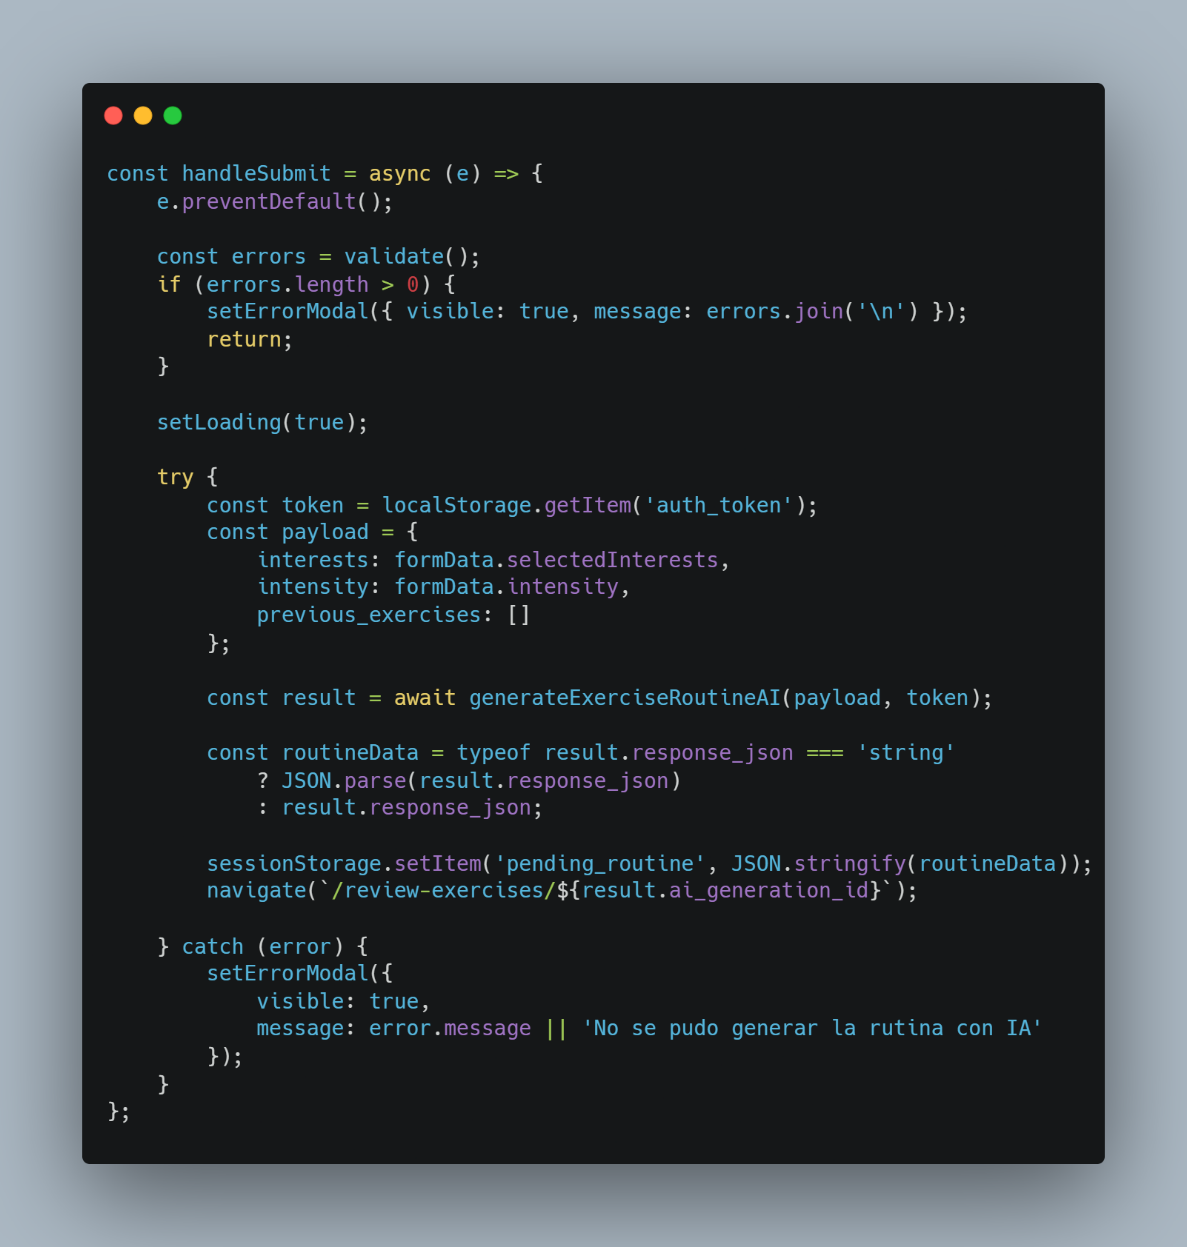
\includegraphics[width=0.9\textwidth]{images/image17.png}
				\end{figure}
				\tblnote
				
				En la aplicación móvil para padres se implementó el componente de panel de progreso del niño. Como evidencia la Figura~\ref{fig:panel}, el componente evalúa condicionalmente el estado de la rutina diaria (\texttt{summary?.daily\_completed}) para mostrar un globo de advertencia (\texttt{warningBalloon}) cuyo color varía entre ámbar y rojo según si la rutina está incompleta o no realizada. La barra de progreso (\texttt{progressBar}) calcula dinámicamente su ancho a partir del porcentaje de rutina completada (\texttt{routine\_pct}), con límites de 0 a 100 aplicados mediante \texttt{Math.min} y \texttt{Math.max}, evitando desbordamientos visuales~\cite{Fowler2002,Hourcade2015}.
				
				\begin{figure}[H]
					\centering
					\caption{Componente React Native del panel de progreso con indicadores condicionales}
					\label{fig:panel}
					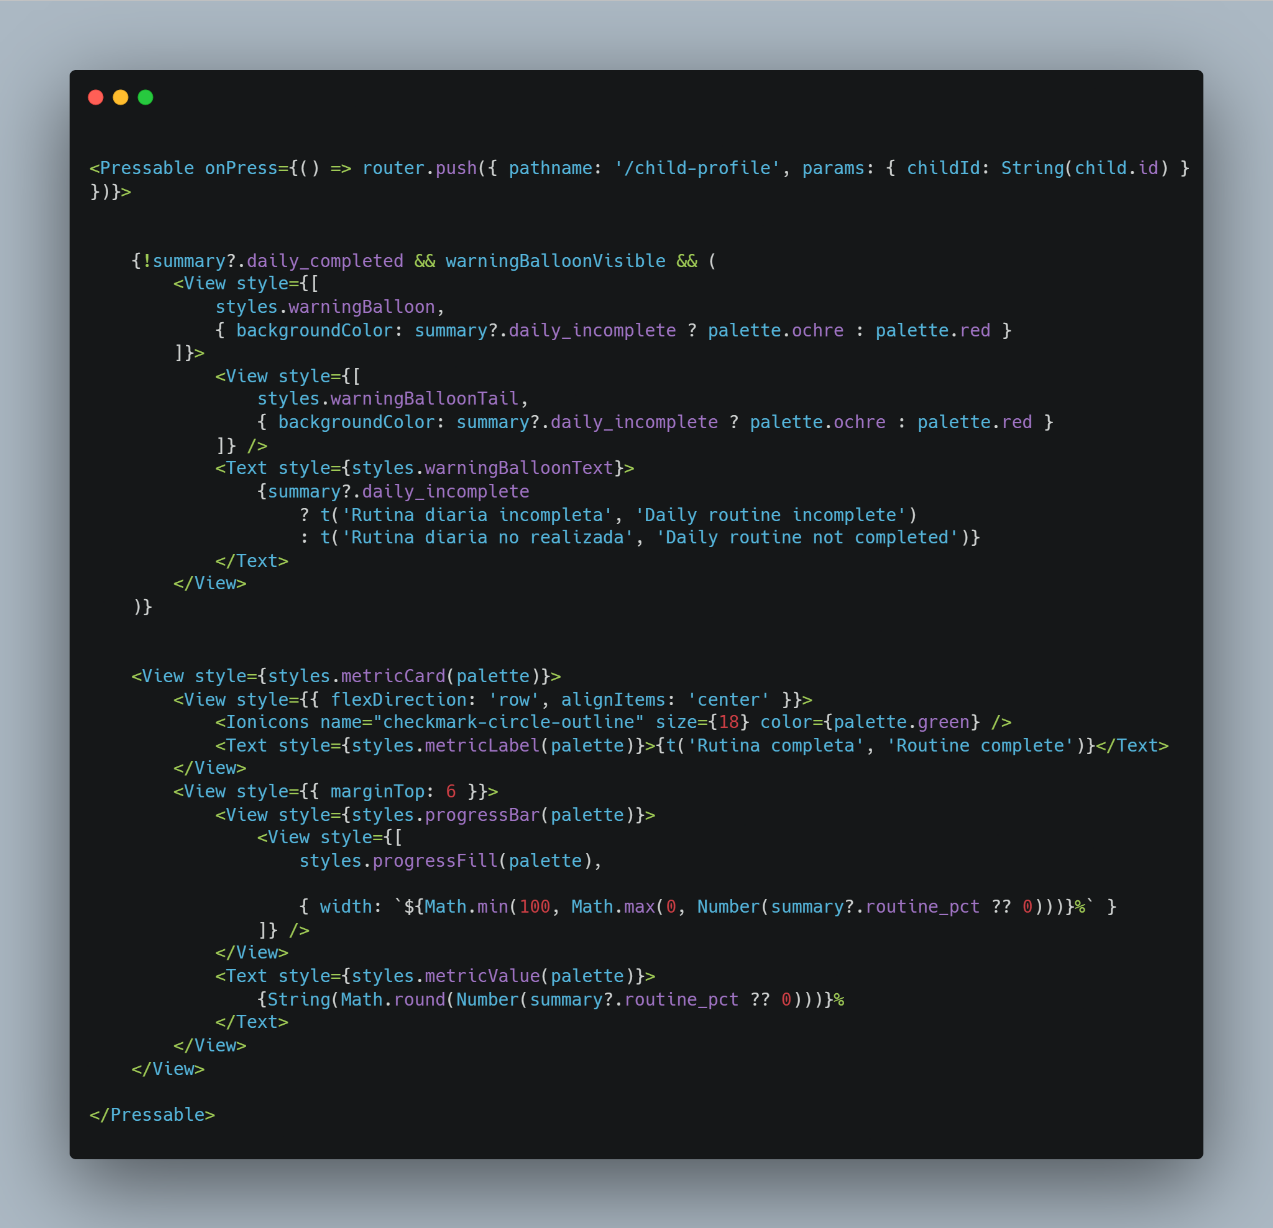
\includegraphics[width=0.9\textwidth]{images/image18.png}
				\end{figure}
				\tblnote
				
				En la aplicación móvil para niños se implementó un verificador de movimiento mediante comparación de fotogramas capturados por cámara. La Figura~\ref{fig:cam} muestra la función \texttt{compareFrames}, que opera directamente sobre las cadenas base64 de dos fotogramas consecutivos sin transmitir datos al servidor, preservando la privacidad del usuario~\cite{LOPDP2021}. El algoritmo muestrea posiciones distribuidas uniformemente a lo largo de la cadena (controladas por \texttt{SAMPLE\_COUNT}) y cuenta diferencias de caracteres entre ambos fotogramas; el resultado pondera el score de caracteres con la diferencia de tamaño de los fotogramas, produciendo un valor normalizado entre 0 y 1 que representa el nivel de movimiento detectado~\cite{Fowler2002}.
				
				\begin{figure}[H]
					\centering
					\caption[Función \texttt{compareFrames} para detección local de movimiento]{Función \texttt{compareFrames} para detección local de movimiento por comparación de fotogramas}
					\label{fig:cam}
					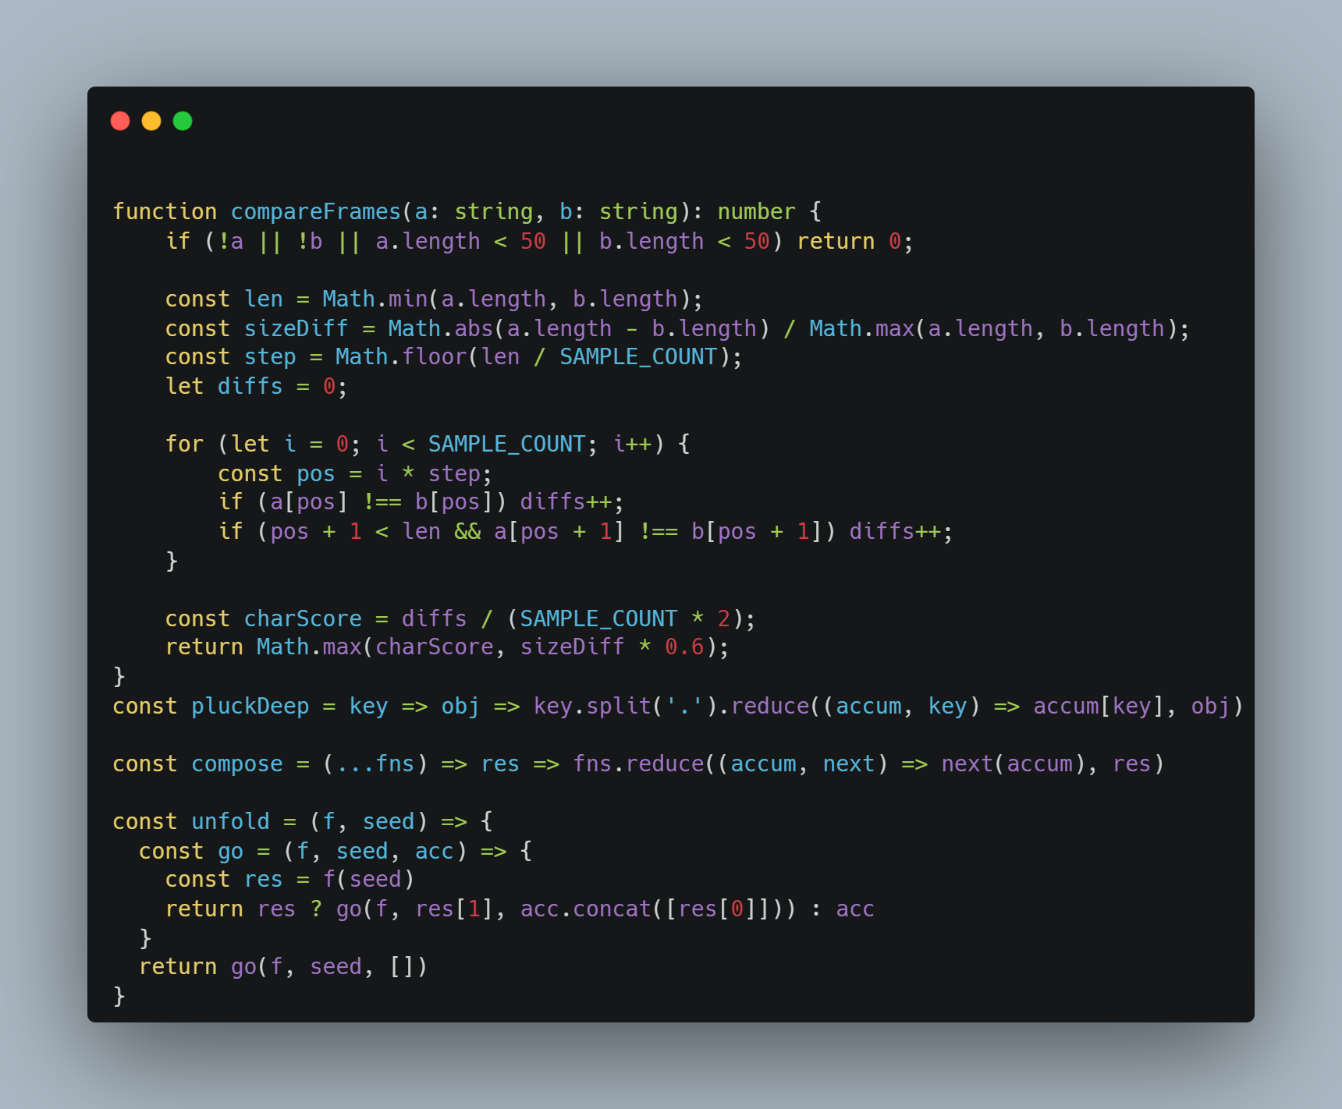
\includegraphics[width=0.9\textwidth]{images/image19.png}
				\end{figure}
				\tblnote
				
			\subsection{Refinamiento del modelo}
				\label{sec:modelref}
				
				En esta fase, denominada \textit{model refinement} por TDDM4IoTS~\cite{GuerreroUlloa2024}, se revisaron y ajustaron los modelos UML generados en la fase~4 a partir de los hallazgos producidos durante la generación e integración del software, siguiendo la observación de la metodología de que la solución funcional no es necesariamente óptima y requiere ajustes de robustez, escalabilidad y reusabilidad~\cite{GuerreroUlloa2024,Fowler2002}.
				
				El diagrama de casos de uso refinado (Figura~\ref{fig:ucref}) incorpora dos cambios estructurales respecto al diagrama original: la explicitación de las relaciones \texttt{«include»} entre los casos de uso del módulo web (CU-06 incluye CU-05, CU-05 incluye CU-04, CU-04 incluye CU-03), lo que formaliza la dependencia secuencial del flujo de validación de contenido; y la adición de una relación \texttt{«depends»} desde CU-08 (Ver rutina diaria) hacia CU-06 (Publicar ejercicio), que captura la dependencia de datos entre el módulo niño y el catálogo publicado por el especialista. Estos ajustes mejoran la trazabilidad del diagrama y lo alinean con la implementación real del sistema.
				
				\begin{figure}[H]
					\centering
					\caption{Diagrama de casos de uso refinado con relaciones \texttt{«include»} y \texttt{«depends»}}
					\label{fig:ucref}
					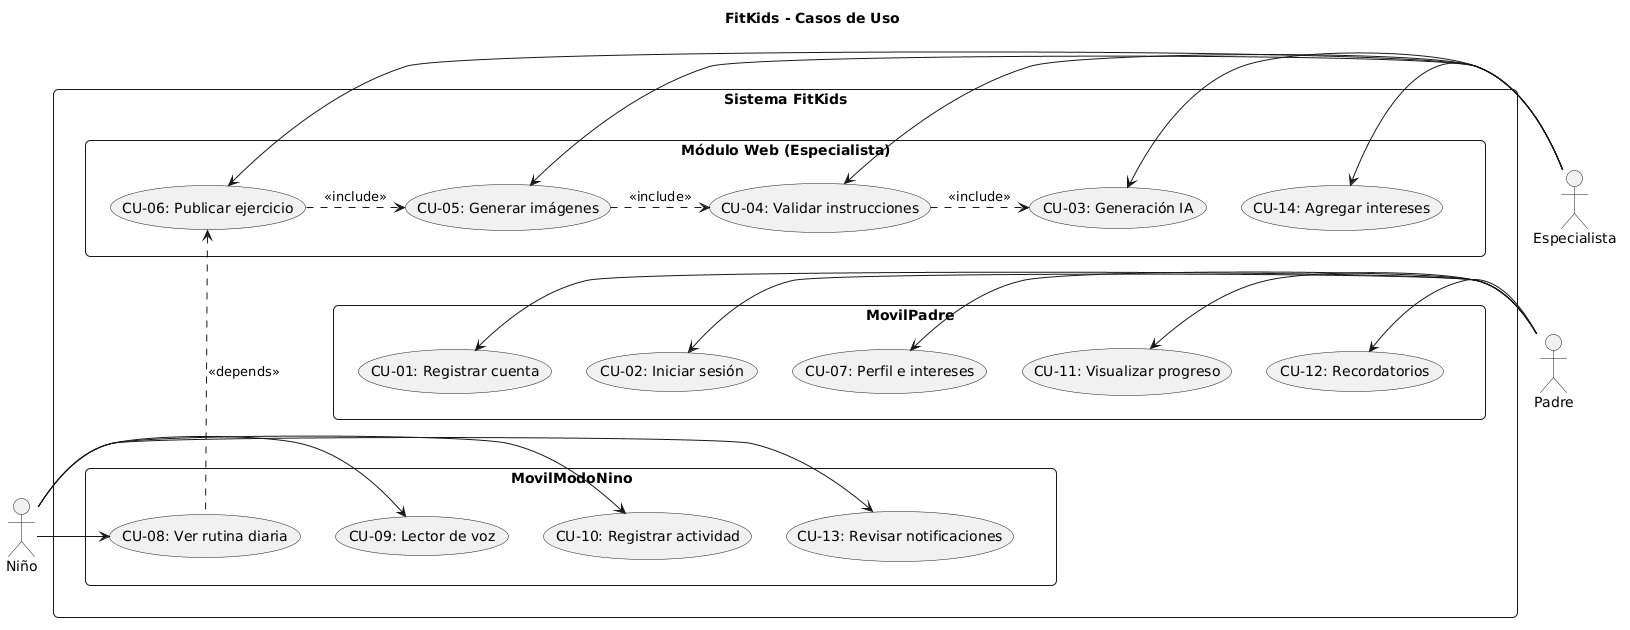
\includegraphics[width=0.9\textwidth]{images/image20.png}
				\end{figure}
				\tblnote
				
				\begin{figure}[H]
					\centering
					\caption{Diagrama de clases refinado con nomenclatura estandarizada y nuevas entidades}
					\label{fig:classref}
					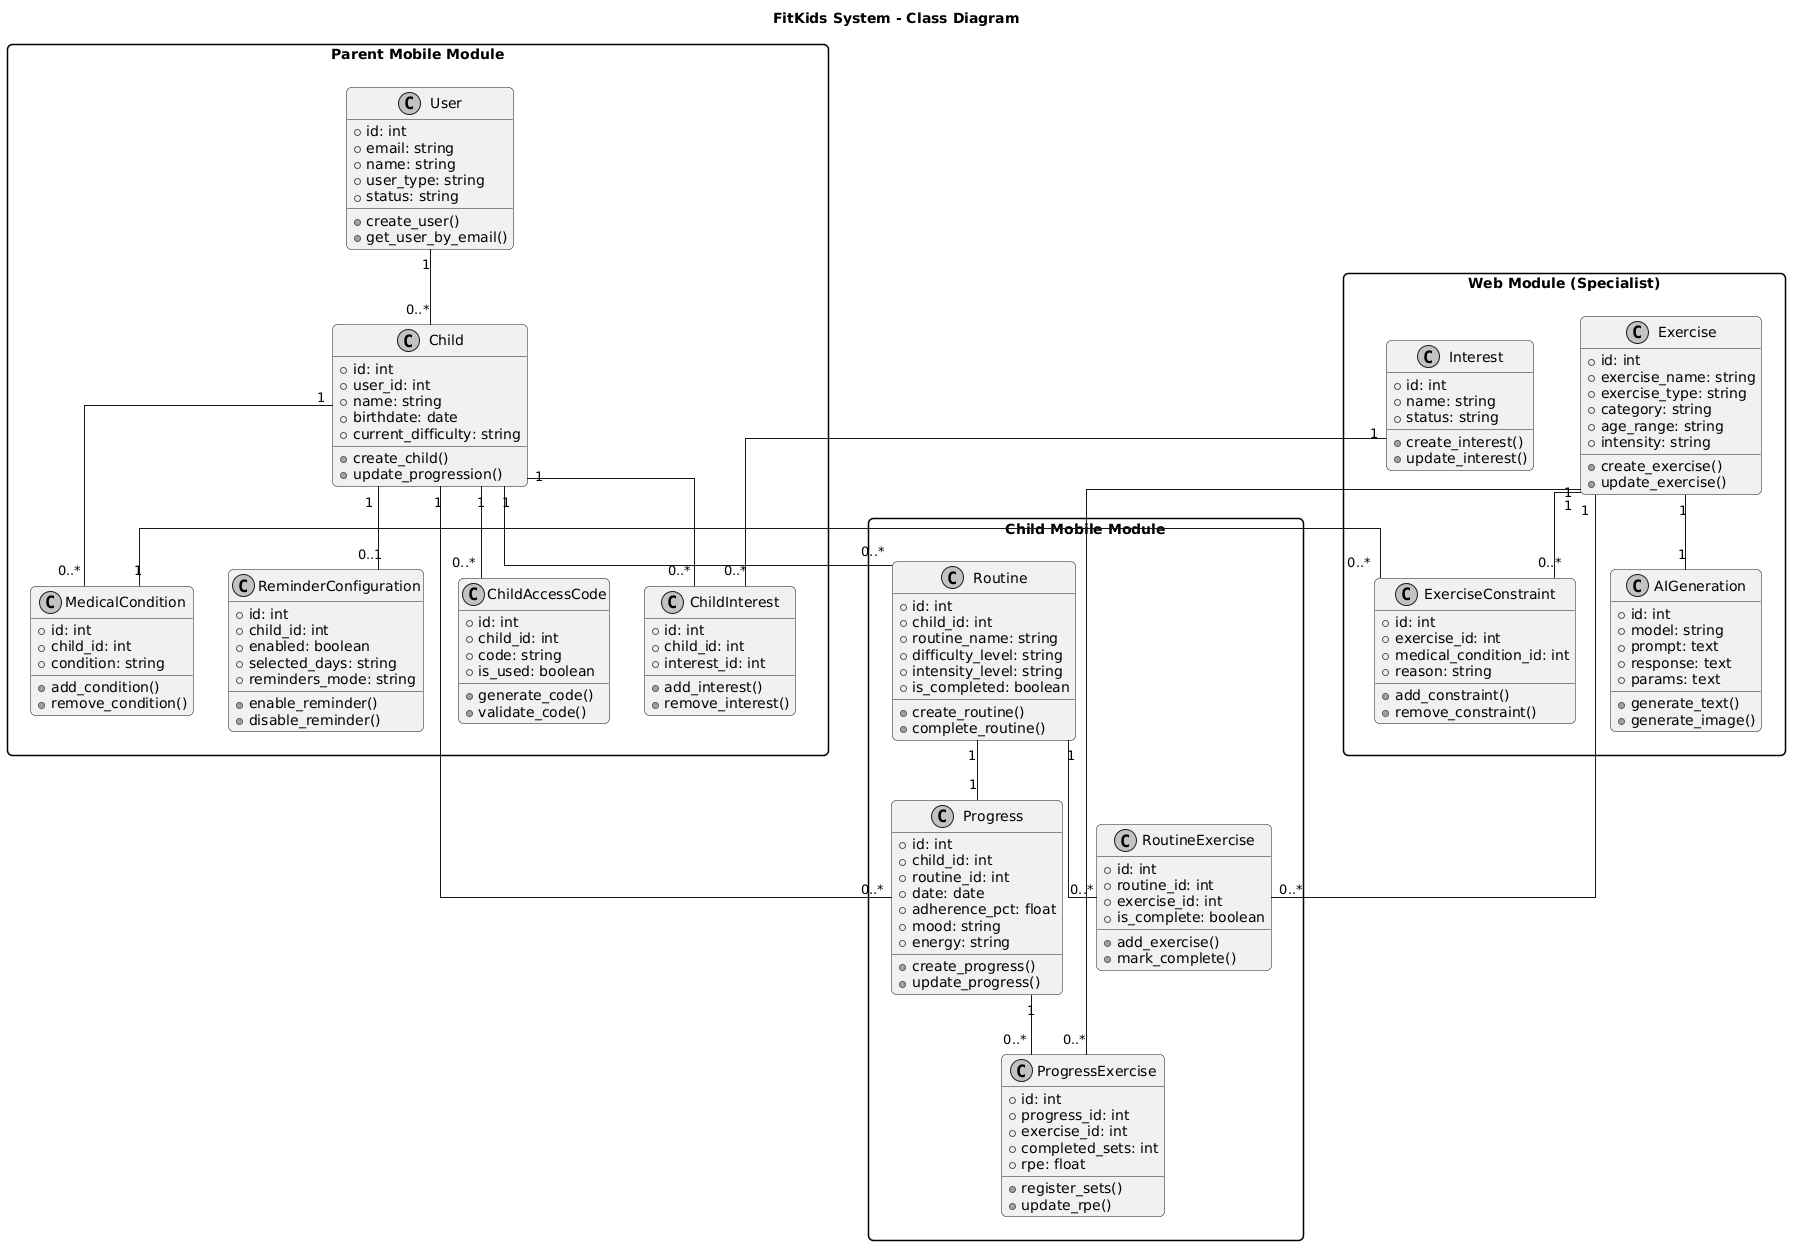
\includegraphics[width=\textwidth]{images/image21.png}
				\end{figure}
				\tblnote
				
				El diagrama de clases refinado (ver Figura~\ref{fig:classref}) incorpora los ajustes derivados de la implementación: se estandarizó la nomenclatura de todas las clases al inglés para mantener coherencia con el código fuente; se añadió el atributo \texttt{age\_range} a la clase \texttt{Exercise} para soportar el filtrado por rango etario requerido en la generación de rutinas; se incorporó el atributo \texttt{rpe} (Rate of Perceived Exertion) en \texttt{ProgressExercise} para registrar el esfuerzo percibido por sesión; y se consolidaron las relaciones entre \texttt{ExerciseConstraint} y \texttt{MedicalCondition} para reflejar el mecanismo de contraindicaciones implementado en el prompt de IA. El diagrama refinado constituye el modelo definitivo del sistema y la base de referencia para el esquema de base de datos en producción~\cite{GuerreroUlloa2024,Fowler2002}.
				
			\subsection{Refinamiento del software}
			\label{sec:softref}
				En esta etapa, denominada \textit{hardware and software deployment} en TDDM4IoTS~\cite{GuerreroUlloa2024}, se realizó la configuración y publicación del sistema en entornos de producción con el objetivo de habilitar su acceso y verificar la integración de sus componentes en condiciones reales. El despliegue se llevó a cabo de forma progresiva en tres frentes: el \textit{backend} se publicó en Render, plataforma de contenedores gestionados con disponibilidad declarada del 99\,\%, cuya capa gratuita mantuvo el costo operativo en cero durante la fase de evaluación~\cite{Wen2023}; la aplicación web fue desplegada en la misma plataforma, quedando accesible para los especialistas pediatras participantes; y la aplicación móvil se distribuyó mediante un APK firmado instalado directamente en los dispositivos Android de los participantes del estudio, estrategia que permitió agilizar la distribución sin depender de los tiempos de revisión de plataformas de distribución de terceros~\cite{GuerreroUlloa2024}. La base de datos PostgreSQL permaneció alojada en Neon, cuya arquitectura \textit{serverless} garantizó la disponibilidad del servicio durante todas las sesiones de evaluación sin requerir aprovisionamiento manual de recursos~\cite{Wen2023}.
				
				La verificación posterior al despliegue se estructuró en torno a tres dimensiones de calidad definidas por la norma ISO/IEC~25010: portabilidad, compatibilidad y fiabilidad~\cite{GuerreroUlloa2024}. Para la portabilidad se comprobó el funcionamiento correcto del sistema en tres navegadores de escritorio distintos y en cuatro modelos de dispositivos Android con versiones de sistema operativo comprendidas entre Android~10 y Android~14. Para la compatibilidad se verificó que el \textit{backend}, las interfaces de usuario y la base de datos se comunicaran correctamente bajo condiciones de red variables, incluyendo conexiones Wi-Fi domésticas y datos móviles 4G. Para la fiabilidad se ejecutaron pruebas de disponibilidad durante 48~horas continuas, sin registrar interrupciones del servicio. Estos resultados confirmaron que el sistema estaba en condiciones operativas adecuadas para iniciar la fase de evaluación con usuarios, estableciendo una base técnica sólida para los indicadores de rendimiento reportados en la sección de Comprobación~(\ref{sec:comprobacion})~\cite{Pressman2019}.
				
			\subsection{Despliegue de software}
			\label{sec:softdep}
				En esta etapa, denominada \textit{hardware and software deployment} en TDDM4IoTS~\cite{GuerreroUlloa2024}, se realizó la configuración y publicación del sistema en entornos de producción con el objetivo de habilitar su acceso y verificar la integración de sus componentes en condiciones reales. El despliegue se llevó a cabo de forma progresiva en tres frentes: el backend se publicó en Render, plataforma de contenedores gestionados con disponibilidad declarada del 99\%, cuya capa gratuita mantuvo el costo operativo en cero durante la fase de evaluación~\cite{Kleppmann2017}; la aplicación web fue desplegada en la misma plataforma, quedando accesible para los especialistas pediatras participantes; y la aplicación móvil se distribuyó mediante su publicación en Google Play Store, lo que permitió su instalación directa en los dispositivos Android de los participantes del estudio~\cite{GuerreroUlloa2024}. Durante esta fase se verificó la compatibilidad del sistema en distintos navegadores y dispositivos móviles, así como la correcta comunicación entre el backend, las interfaces de usuario y la base de datos en Neon, atendiendo a los atributos de portabilidad y compatibilidad del modelo de calidad ISO/IEC~25010~\cite{GuerreroUlloa2024}.
				
			\subsection{Evaluación de entregables}
			\label{delEval}
				Las Tablas~\ref{tab:cpf01} a~\ref{tab:cpnf04} documentan los 16~casos de prueba aplicados sobre el sistema FitKids: 12~funcionales (CP-F01 a CP-F12), que verifican el comportamiento de cada requisito funcional en condiciones reales de uso, y 4~no funcionales (CP-NF01 a CP-NF04), que verifican los atributos de calidad del sistema conforme a los criterios definidos en RNF1 a RNF4~\cite{GuerreroUlloa2024}. Los casos funcionales se organizan en tres grupos temáticos: acceso y gestión de cuenta (CP-F01 y CP-F02), flujo de contenido del módulo web (CP-F03 a CP-F06) y flujo de actividad del módulo móvil (CP-F07 a CP-F12).
				
				La ejecución de los casos de prueba siguió el principio de evaluación incremental establecido por la metodología TDDM4IoTS, en el que cada entregable parcial se valida antes de avanzar hacia la fase siguiente, de modo que los defectos se detectan y corrigen en su punto de origen sin propagarse a los componentes posteriores~\cite{GuerreroUlloa2024,Pressman2019}.
				
				Los casos del grupo de acceso verificaron la integridad del flujo de autenticación para los tres perfiles de usuario del sistema (padre, niño y especialista). Los del flujo de contenido web validaron la cadena completa de generación, revisión, aprobación y publicación de ejercicios, que constituye el núcleo del modelo \textit{human-in-the-loop} del sistema. Los del flujo de actividad móvil cubrieron las funcionalidades de mayor impacto en la experiencia del niño: generación de rutina personalizada, lector de voz, registro de tiempo, visualización del progreso y gestión de recordatorios~\cite{GuerreroUlloa2024}.
				
				Los cuatro casos no funcionales verificaron, respectivamente, que las rutinas generadas se mantuvieran dentro de los límites de intensidad seguros para la edad, que el lenguaje empleado fuera comprensible para niños de 6 a 11~años, que la navegación entre secciones resultara fluida sin errores, y que el acceso a los datos del niño permaneciera restringido al adulto responsable, atributos alineados con los factores de calidad en uso de la norma ISO/IEC~25010~\cite{GuerreroUlloa2024}. La totalidad de los 16~casos resultó en estado «Superado», lo que establece la base empírica para los indicadores de cumplimiento de requisitos y cobertura de pruebas presentados en la sección de Comprobación~(\ref{sec:comprobacion}).
				
				\begin{table}[H]
					\centering\small
					\caption{Caso de prueba CP-F01: Registro de cuenta de usuario}
					\label{tab:cpf01}
					\begin{tabular}{p{3cm}p{12.0cm}}
						\hline
						\textbf{Campo} & \textbf{Detalle}\\
						\hline
						Identificador & CP-F01\\
						Requisito asociado & RF5 --- Supervisión adulta (acceso y autenticación)\\
						Versión & V1.0\\
						Prioridad & Alta\\
						Descripción & Validar que el sistema permita registrar una cuenta con datos válidos y almacene la contraseña en hash bcrypt.\\
						Precondiciones & No debe haber una sesión de usuario activa en el dispositivo.\\
						Pasos de prueba & 1. Abrir la aplicación móvil o el módulo web.\newline 2. Seleccionar ``Registrar cuenta''.\newline 3. Completar el formulario con nombre, correo y contraseña.\newline 4. Confirmar el registro.\\
						Datos de prueba & Nombre: Valeska; Correo: holamundo@mail.com; Contraseña: Password123\\
						Resultado esperado & El sistema registra al usuario, almacena la contraseña en hash bcrypt y muestra confirmación de cuenta creada.\\
						Resultado obtenido & El usuario se registró correctamente y se mostró el mensaje de confirmación.\\
						Estado & Superado\\
						\hline
					\end{tabular}
				\end{table}
				\tblnote
				
				\begin{table}[H]
					\centering\small
					\caption{Caso de prueba CP-F02: Inicio de sesión de usuario}
					\label{tab:cpf02}
					\begin{tabular}{p{3cm}p{12.0cm}}
						\hline
						\textbf{Campo} & \textbf{Detalle}\\
						\hline
						Identificador & CP-F02\\
						Requisito asociado & RF5 --- Supervisión adulta (acceso y autenticación)\\
						Versión & V1.0\\
						Prioridad & Alta\\
						Descripción & Validar que el sistema permita iniciar sesión con credenciales válidas y deniegue el acceso con credenciales incorrectas.\\
						Precondiciones & No debe haber sesión activa; la cuenta debe existir en el sistema.\\
						Pasos de prueba & 1. Abrir la aplicación móvil o el módulo web.\newline 2. Ingresar correo y contraseña.\newline 3. Presionar ``Iniciar sesión''.\\
						Datos de prueba & Correo: holamundo@mail.com; Contraseña: Password123\\
						Resultado esperado & El sistema autentica al usuario y muestra el menú principal correspondiente a su perfil.\\
						Resultado obtenido & El acceso fue exitoso y se mostró el menú principal.\\
						Estado & Superado\\
						\hline
					\end{tabular}
				\end{table}
				\tblnote
				
				\textbf{Flujo de contenido del módulo web --- especialista.} Los casos CP-F03 a CP-F06 verifican la cadena de validación de contenido: registro del perfil del niño como parámetro de personalización (CP-F03), generación de ejercicios por IA con estado ``Pendiente de revisión'' (CP-F04), revisión y aprobación clínica individual (CP-F05) y publicación al catálogo activo (CP-F06). Esta secuencia es prerrequisito para que el módulo móvil pueda generar rutinas.
								
				\begin{table}[H]
					\centering\small
					\caption{Caso de prueba CP-F03: Gestión del perfil e intereses del niño}
					\label{tab:cpf03}
					\begin{tabular}{p{3cm}p{12.0cm}}
						\hline
						\textbf{Campo} & \textbf{Detalle}\\
						\hline
						Identificador & CP-F03\\
						Requisito asociado & RF3 --- Adaptación a gustos del niño; RF5 --- Supervisión adulta\\
						Versión & V1.0\\
						Prioridad & Alta\\
						Descripción & Validar el registro y actualización del perfil del niño con sus intereses deportivos.\\
						Precondiciones & El padre debe tener sesión iniciada en la aplicación móvil.\\
						Pasos de prueba & 1. Ir a ``Agregar niño''.\newline 2. Completar datos (apodo, rango de edad, género, altura, peso, condiciones).\newline 3. Seleccionar intereses deportivos.\newline 4. Guardar y finalizar.\\
						Datos de prueba & Apodo: Niño1; Edad: 6--7 años; Peso: 28,5 kg; Intensidad: Aventurero; Intereses: Atletismo, Fútbol\\
						Resultado esperado & El sistema guarda el perfil del niño y registra sus intereses para personalización de rutinas.\\
						Resultado obtenido & El perfil se guardó y los intereses quedaron registrados correctamente.\\
						Estado & Superado\\
						\hline
					\end{tabular}
				\end{table}
				\tblnote
				
				\begin{table}[H]
					\centering\small
					\caption{Caso de prueba CP-F04: Generación de ejercicios mediante inteligencia artificial}
					\label{tab:cpf04}
					\begin{tabular}{p{3cm}p{12.0cm}}
						\hline
						\textbf{Campo} & \textbf{Detalle}\\
						\hline
						Identificador & CP-F04\\
						Requisito asociado & RF2 --- Validación de ejercicios por especialistas\\
						Versión & V1.0\\
						Prioridad & Alta\\
						Descripción & Validar que el especialista solicite la generación de ejercicios con IA y que los resultados queden en estado ``Pendiente de revisión''.\\
						Precondiciones & Especialista con sesión iniciada en el módulo web; API de Gemini disponible.\\
						Pasos de prueba & 1. Abrir el módulo web.\newline 2. Ir a ``Generar ejercicios con IA''.\newline 3. Seleccionar interés y rango de edad.\newline 4. Presionar ``Generar Ejercicios''.\newline 5. Revisar el listado de ``Pendientes''.\\
						Datos de prueba & Rango: 8--9 años; Interés: Atletismo\\
						Resultado esperado & El sistema genera ejercicios y los registra con estado ``Pendiente de revisión''.\\
						Resultado obtenido & Se generaron ejercicios y quedaron en estado pendiente.\\
						Estado & Superado\\
						\hline
					\end{tabular}
				\end{table}
				\tblnote
				
				\begin{table}[H]
					\centering\small
					\caption{Caso de prueba CP-F05: Revisión y validación de ejercicios por especialista}
					\label{tab:cpf05}
					\begin{tabular}{p{3cm}p{12.0cm}}
						\hline
						\textbf{Campo} & \textbf{Detalle}\\
						\hline
						Identificador & CP-F05\\
						Requisito asociado & RF2 --- Validación de ejercicios por especialistas; RNF1 --- Seguridad clínica\\
						Versión & V1.0\\
						Prioridad & Alta\\
						Descripción & Validar que el especialista revise el contenido e imagen de un ejercicio generado y lo apruebe o rechace individualmente.\\
						Precondiciones & Existencia de ejercicios en estado ``Pendiente de revisión''.\\
						Pasos de prueba & 1. Ingresar a ``Pendientes''.\newline 2. Seleccionar un ejercicio.\newline 3. Revisar contenido e imagen.\newline 4. Presionar ``Aprobar'' o ``Rechazar''.\\
						Datos de prueba & Ejercicio: ``Saltos de estrella''\\
						Resultado esperado & El ejercicio cambia al estado ``Aprobado'' o ``Rechazado'' y la acción queda registrada en la base de datos.\\
						Resultado obtenido & El ejercicio fue aprobado y quedó registrado correctamente.\\
						Estado & Superado\\
						\hline
					\end{tabular}
				\end{table}
				\tblnote
				
				\begin{table}[H]
					\centering\small
					\caption{Caso de prueba CP-F06: Publicación de ejercicios validados}
					\label{tab:cpf06}
					\begin{tabular}{p{3cm}p{12.0cm}}
						\hline
						\textbf{Campo} & \textbf{Detalle}\\
						\hline
						Identificador & CP-F06\\
						Requisito asociado & RF1 --- Generación de rutinas validadas por especialistas\\
						Versión & V1.0\\
						Prioridad & Media\\
						Descripción & Validar que el especialista publique al catálogo los ejercicios aprobados con sus imágenes.\\
						Precondiciones & Existencia de ejercicios en estado ``Aprobado'' con imagen generada.\\
						Pasos de prueba & 1. Presionar ``Publicar \textit{N} ejercicios con imágenes''.\\
						Datos de prueba & Ejercicio aprobado: ``Saltos de estrella''\\
						Resultado esperado & Los ejercicios quedan disponibles en el catálogo activo para la generación de rutinas.\\
						Resultado obtenido & El ejercicio se publicó correctamente en el catálogo.\\
						Estado & Superado\\
						\hline
					\end{tabular}
				\end{table}
				\tblnote
				
				\textbf{Flujo de actividad del módulo móvil.} Los casos CP-F07 a CP-F12 verifican el ciclo de uso del niño y del padre: generación de rutina personalizada (CP-F07), reproducción de instrucciones por voz (CP-F08), registro automático del tiempo de actividad (CP-F09), visualización del progreso (CP-F10) y gestión de recordatorios push, tanto en su configuración (CP-F11) como en su entrega (CP-F12).
				
				\begin{table}[H]
					\centering\small
					\caption{Caso de prueba CP-F07: Generación de rutina personalizada}
					\label{tab:cpf07}
					\begin{tabular}{p{3cm}p{12.0cm}}
						\hline
						\textbf{Campo} & \textbf{Detalle}\\
						\hline
						Identificador & CP-F07\\
						Requisito asociado & RF1 --- Generación de rutinas; RF3 --- Adaptación a gustos; RF6 --- Rutinas en el hogar\\
						Versión & V1.0\\
						Prioridad & Alta\\
						Descripción & Validar que el sistema genere una rutina diaria personalizada acorde al perfil e intereses del niño, ejecutable en el hogar sin equipamiento.\\
						Precondiciones & Sesión iniciada; perfil del niño completo; ejercicios publicados disponibles en el catálogo.\\
						Pasos de prueba & 1. Ir a ``Ver rutina'' en el modo niño.\newline 2. Seleccionar interés deportivo.\newline 3. Confirmar generación.\\
						Datos de prueba & Interés: Atletismo\\
						Resultado esperado & El sistema genera una rutina con ejercicios adecuados al perfil, intereses y contexto de hogar.\\
						Resultado obtenido & Rutina generada correctamente con ejercicios acordes.\\
						Estado & Superado\\
						\hline
					\end{tabular}
				\end{table}
				\tblnote
				
				\begin{table}[H]
					\centering\small
					\caption{Caso de prueba CP-F08: Reproducción de instrucciones con lector de voz}
					\label{tab:cpf08}
					\begin{tabular}{p{3cm}p{12.0cm}}
						\hline
						\textbf{Campo} & \textbf{Detalle}\\
						\hline
						Identificador & CP-F08\\
						Requisito asociado & RF9 --- Lector de voz; RNF2 --- Adecuación del lenguaje\\
						Versión & V1.0\\
						Prioridad & Media\\
						Descripción & Validar que el sistema reproduzca mediante síntesis de voz las instrucciones del ejercicio activo sin requerir acción adicional del usuario.\\
						Precondiciones & Rutina diaria disponible; dispositivo con audio habilitado.\\
						Pasos de prueba & 1. Abrir un ejercicio de la rutina.\newline 2. Presionar ``Escuchar''.\newline 3. Verificar reproducción completa del texto descriptivo.\\
						Datos de prueba & Ejercicio: ``Saltos de estrella''\\
						Resultado esperado & Se reproduce el audio con las instrucciones completas del ejercicio sin truncamientos.\\
						Resultado obtenido & Audio reproducido correctamente.\\
						Estado & Superado\\
						\hline
					\end{tabular}
				\end{table}
				\tblnote
				
				\begin{table}[H]
					\centering\small
					\caption{Caso de prueba CP-F09: Registro del tiempo de actividad física}
					\label{tab:cpf09}
					\begin{tabular}{p{3cm}p{12.0cm}}
						\hline
						\textbf{Campo} & \textbf{Detalle}\\
						\hline
						Identificador & CP-F09\\
						Requisito asociado & RF7 --- Registro del tiempo de actividad\\
						Versión & V1.0\\
						Prioridad & Alta\\
						Descripción & Validar el registro automático del tiempo dedicado a la actividad física y su persistencia en el historial del niño.\\
						Precondiciones & Rutina diaria disponible y ejercicio en ejecución.\\
						Pasos de prueba & 1. Iniciar la rutina.\newline 2. Completar un ejercicio presionando ``¡Ejercicio completado!''.\newline 3. Finalizar la sesión.\\
						Datos de prueba & Tiempo registrado: 12 minutos\\
						Resultado esperado & El sistema guarda el tiempo asociado al día del niño y lo refleja en el progreso en menos de 5 segundos.\\
						Resultado obtenido & Tiempo guardado correctamente y visible en el historial de progreso.\\
						Estado & Superado\\
						\hline
					\end{tabular}
				\end{table}
				\tblnote
				
				\begin{table}[H]
					\centering\small
					\caption{Caso de prueba CP-F10: Visualización del progreso del niño}
					\label{tab:cpf10}
					\begin{tabular}{p{3cm}p{12.0cm}}
						\hline
						\textbf{Campo} & \textbf{Detalle}\\
						\hline
						Identificador & CP-F10\\
						Requisito asociado & RF8 --- Visualización del progreso\\
						Versión & V1.0\\
						Prioridad & Alta\\
						Descripción & Validar que el sistema muestre al padre el historial de actividad con estados diferenciados (Completada / No realizada) y tiempo acumulado.\\
						Precondiciones & El padre debe tener sesión iniciada; existencia de registros de actividad previos.\\
						Pasos de prueba & 1. Ingresar a ``Ver progreso''.\newline 2. Seleccionar período de consulta.\newline 3. Revisar historial por día.\\
						Datos de prueba & Día actual: 3 ejercicios, 2 completados, 1 incompleto\\
						Resultado esperado & El sistema muestra el cumplimiento y el tiempo acumulado con estados visuales diferenciados.\\
						Resultado obtenido & Progreso visualizado correctamente con indicadores de estado.\\
						Estado & Superado\\
						\hline
					\end{tabular}
				\end{table}
				\tblnote
				
				\begin{table}[H]
					\centering\small
					\caption{Caso de prueba CP-F11: Configuración de recordatorios de actividad física}
					\label{tab:cpf11}
					\begin{tabular}{p{3cm}p{12.0cm}}
						\hline
						\textbf{Campo} & \textbf{Detalle}\\
						\hline
						Identificador & CP-F11\\
						Requisito asociado & RF4 --- Recordatorios de actividad física; RF5 --- Supervisión adulta\\
						Versión & V1.0\\
						Prioridad & Media\\
						Descripción & Validar que el padre configure recordatorios push con día, hora y frecuencia, y que el sistema los almacene correctamente.\\
						Precondiciones & Padre con sesión iniciada; permisos de notificación push habilitados en el dispositivo.\\
						Pasos de prueba & 1. Ir a ``Recordatorios''.\newline 2. Activar el interruptor de recordatorio.\newline 3. Seleccionar días y hora.\newline 4. Presionar ``Guardar configuración''.\\
						Datos de prueba & Hora: 18:00; Días: lunes a viernes; Cantidad: 1 recordatorio al día\\
						Resultado esperado & El sistema guarda la configuración y activa el servicio de notificaciones push en OneSignal.\\
						Resultado obtenido & Configuración guardada y recordatorio activado correctamente.\\
						Estado & Superado\\
						\hline
					\end{tabular}
				\end{table}
				\tblnote
				
				\begin{table}[H]
					\centering\small
					\caption{Caso de prueba CP-F12: Recepción de recordatorios}
					\label{tab:cpf12}
					\begin{tabular}{p{3cm}p{12.0cm}}
						\hline
						\textbf{Campo} & \textbf{Detalle}\\
						\hline
						Identificador & CP-F12\\
						Requisito asociado & RF4 --- Recordatorios de actividad física\\
						Versión & V1.0\\
						Prioridad & Media\\
						Descripción & Validar que el sistema envíe la notificación push en el horario configurado y que el dispositivo la reciba aunque la app esté en segundo plano.\\
						Precondiciones & Recordatorio habilitado; dispositivo con notificaciones activas y conectividad disponible.\\
						Pasos de prueba & 1. Esperar la hora configurada.\newline 2. Verificar recepción de la notificación en el dispositivo.\newline 3. Abrir la aplicación desde la notificación.\\
						Datos de prueba & Hora programada: 18:00\\
						Resultado esperado & La notificación se recibe en el horario configurado y al abrirla redirige a la pantalla de rutina.\\
						Resultado obtenido & Notificación recibida y redirección correcta hacia la rutina del día.\\
						Estado & Superado\\
						\hline
					\end{tabular}
				\end{table}
				\tblnote
				
				\textbf{Requisitos no funcionales.} Los casos CP-NF01 a CP-NF04 verifican los atributos de calidad que determinan la viabilidad clínica y legal del sistema: seguridad clínica de las rutinas generadas (CP-NF01), adecuación del lenguaje al rango etario (CP-NF02), usabilidad de navegación con umbral de tres interacciones (CP-NF03) y restricción de acceso a los datos del menor (CP-NF04)~\cite{LOPDP2021,GuerreroUlloa2024}.
				
				\begin{table}[H]
					\centering\small
					\caption{Caso de prueba CP-NF01: Seguridad clínica}
					\label{tab:cpnf01}
					\begin{tabular}{p{3cm}p{12.0cm}}
						\hline
						\textbf{Campo} & \textbf{Detalle}\\
						\hline
						Identificador & CP-NF01\\
						Requisito asociado & RNF1 --- Seguridad clínica\\
						Versión & V1.0\\
						Prioridad & Alta\\
						Descripción & Validar que las rutinas generadas no excedan los límites de duración e intensidad definidos por los especialistas para el rango de edad del niño.\\
						Precondiciones & Perfil infantil registrado; parámetros de límites configurados por el especialista.\\
						Pasos de prueba & 1. Ingresar al perfil del niño.\newline 2. Generar una rutina personalizada.\newline 3. Revisar duración e intensidad de cada ejercicio.\newline 4. Comparar con los límites definidos por el especialista.\\
						Datos de prueba & Edad: 7 años; Interés: Atletismo\\
						Resultado esperado & Ningún ejercicio de la rutina supera los límites de tiempo e intensidad definidos.\\
						Resultado obtenido & Rutina dentro de los límites permitidos.\\
						Estado & Superado\\
						\hline
					\end{tabular}
				\end{table}
				\tblnote
				
				\begin{table}[H]
					\centering\small
					\caption{Caso de prueba CP-NF02: Adecuación del lenguaje}
					\label{tab:cpnf02}
					\begin{tabular}{p{3cm}p{12.0cm}}
						\hline
						\textbf{Campo} & \textbf{Detalle}\\
						\hline
						Identificador & CP-NF02\\
						Requisito asociado & RNF2 --- Adecuación del lenguaje\\
						Versión & V1.0\\
						Prioridad & Media\\
						Descripción & Validar que el contenido textual de las instrucciones y mensajes del modo niño sea claro y comprensible para el rango etario de 6 a 11 años, sin tecnicismos ni abreviaturas no explicadas.\\
						Precondiciones & App instalada; acceso a las pantallas del modo niño con rutina disponible.\\
						Pasos de prueba & 1. Ingresar a una rutina en modo niño.\newline 2. Revisar instrucciones de ejercicios.\newline 3. Revisar mensajes motivacionales.\newline 4. Evaluar comprensión con usuario de 9 años sin asistencia.\\
						Datos de prueba & Perfil niño: 9 años; pantallas de rutina y mensajes motivacionales\\
						Resultado esperado & El contenido es claro, simple y comprensible sin necesidad de asistencia adulta para el rango etario superior.\\
						Resultado obtenido & Contenido adecuado para la edad; el niño evaluado comprendió todas las instrucciones.\\
						Estado & Superado\\
						\hline
					\end{tabular}
				\end{table}
				\tblnote
				
				\begin{table}[H]
					\centering\small
					\caption{Caso de prueba CP-NF03: Usabilidad de navegación}
					\label{tab:cpnf03}
					\begin{tabular}{p{3cm}p{12.0cm}}
						\hline
						\textbf{Campo} & \textbf{Detalle}\\
						\hline
						Identificador & CP-NF03\\
						Requisito asociado & RNF3 --- Usabilidad de navegación\\
						Versión & V1.0\\
						Prioridad & Alta\\
						Descripción & Validar que el usuario navegue entre las secciones principales del sistema en tres interacciones o menos, sin requerir instrucciones previas.\\
						Precondiciones & Usuario autenticado; aplicación funcional.\\
						Pasos de prueba & 1. Acceder a Inicio.\newline 2. Ir a Rutina.\newline 3. Volver a Inicio.\newline 4. Ir a Progreso.\newline 5. Regresar al menú principal.\\
						Datos de prueba & Usuario padre con perfil infantil creado\\
						Resultado esperado & Navegación fluida entre secciones principales sin errores ni confusión; flujo completado en tres interacciones o menos.\\
						Resultado obtenido & Navegación correcta en todas las secciones evaluadas.\\
						Estado & Superado\\
						\hline
					\end{tabular}
				\end{table}
				\tblnote
				
				\begin{table}[H]
					\centering\small
					\caption{Caso de prueba CP-NF04: Privacidad y protección de datos}
					\label{tab:cpnf04}
					\begin{tabular}{p{3cm}p{12.0cm}}
						\hline
						\textbf{Campo} & \textbf{Detalle}\\
						\hline
						Identificador & CP-NF04\\
						Requisito asociado & RNF4 --- Privacidad y protección de datos\\
						Versión & V1.0\\
						Prioridad & Alta\\
						Descripción & Validar que el acceso a los datos del niño esté restringido al adulto responsable autenticado y que las contraseñas se almacenen en formato hash bcrypt.\\
						Precondiciones & Perfil infantil creado; sesión activa del adulto responsable.\\
						Pasos de prueba & 1. Cerrar sesión.\newline 2. Intentar acceder a los datos del niño sin sesión activa.\newline 3. Iniciar sesión con credenciales válidas.\newline 4. Acceder nuevamente al perfil del niño.\\
						Datos de prueba & Datos personales y rutinas del niño registrado\\
						Resultado esperado & Sin sesión: error HTTP 401, acceso denegado. Con sesión válida: acceso permitido.\\
						Resultado obtenido & Restricción aplicada correctamente en ambos escenarios.\\
						Estado & Superado\\
						\hline
					\end{tabular}
				\end{table}
				\tblnote
				
				La totalidad de los 16 casos de prueba resultó en estado ``Superado'', lo que confirma que el sistema cumple con el comportamiento especificado tanto en sus requisitos funcionales como en los atributos de calidad definidos. Este resultado, junto con los 38 casos unitarios y las 6 pruebas de integración documentados en las secciones anteriores, establece la base empírica para los indicadores de cumplimiento de requisitos y cobertura de pruebas que se presentan en la sección de Comprobación~(\ref{sec:comprobacion})~\cite{GuerreroUlloa2024}.
				
				\subsection{Mantenimiento}
				\label{sec:mant}
					El mantenimiento del sistema FitKids se plantea como una proyección a futuro, dado que su estado actual corresponde al de un prototipo funcional. La metodología TDDM4IoTS reconoce explícitamente esta fase como parte del ciclo de vida del sistema, señalando que el mantenimiento de un sistema IoT combina la complejidad del mantenimiento de software con la del hardware, y que requiere planificación preventiva desde el diseño~\cite{GuerreroUlloa2024}. En concordancia, la Tabla~\ref{tab:mantenimiento} detalla los cuatro tipos de mantenimiento previstos según la clasificación clásica de la ingeniería de software~\cite{Pressman2019}: correctivo, adaptativo, evolutivo y preventivo.
					
					\begin{table}[H]
						\centering\small
						\caption{Plan de mantenimiento de la aplicación FitKids}
						\label{tab:mantenimiento}
						\begin{tabular}{p{2.6cm}p{2.8cm}p{3.8cm}p{2.4cm}p{2.4cm}}
							\hline
							\textbf{Tipo} & \textbf{Descripción} & \textbf{Actividades principales} & \textbf{Frecuencia} & \textbf{Responsable}\\
							\hline
							Correctivo & Corrección de errores detectados durante el uso del sistema & Identificación de fallos, corrección de bugs, actualización de código, pruebas de verificación & Según incidencias & Equipo técnico\\
							Adaptativo & Actualización frente a cambios tecnológicos o del entorno & Actualización de librerías, compatibilidad con nuevas versiones de Android, ajustes en APIs externas (IA, notificaciones) & Cada 3--6 meses & Desarrollador\\
							Evolutivo & Mejora continua e incorporación de nuevas funcionalidades & Implementación de nuevas características, mejoras en UI/UX, optimización de rendimiento & Según requerimientos & Equipo de desarrollo\\
							Preventivo & Prevención de fallos y garantía de estabilidad del sistema & Revisión de código, pruebas periódicas, monitoreo del sistema, respaldo de base de datos & Mensual & Equipo técnico\\
							\hline
						\end{tabular}
					\end{table}
					\tblnote
		\section{Comprobación}
		\label{sec:comprobacion}
			Esta sección presenta los resultados obtenidos al aplicar los once indicadores de evaluación formalizados en el apartado~3.9 del Capítulo~III. La organización sigue el mismo orden y nomenclatura declarados en la metodología, lo que garantiza la trazabilidad directa entre cada indicador definido y su resultado correspondiente. Los criterios de aceptación y las ecuaciones empleadas se mantienen sin modificación respecto a lo declarado, en consonancia con los lineamientos institucionales para los proyectos tecnológicos de la Unidad de Integración Curricular~\cite{GuerreroUlloa2024}.
					
			\subsection{Cumplimiento de requisitos}
			\label{subsec:cr}
				Para evaluar el cumplimiento del alcance funcional y no funcional se construyó la matriz de trazabilidad que vincula cada uno de los 16~requisitos definidos en el análisis ---9~funcionales y 7~no funcionales--- con los componentes implementados y los casos de prueba que los validan~\cite{Pressman2019,Fowler2002}. Aplicando la Ecuación~\eqref{ec:cr} declarada en la metodología, donde $R_c$ es el número de requisitos cubiertos y $R_t$ el número total de requisitos definidos:
				
				\begin{equation}
					CR = \frac{16}{16} \times 100\% = 100\%
				\end{equation}
				
				La totalidad de los requisitos definidos fue implementada y verificada mediante los casos de prueba documentados en las secciones~4.1.5 y~4.1.10. El valor obtenido (100\%) supera ampliamente el umbral de aceptación establecido ($CR \geq 95\%$), lo que evidencia que el alcance comprometido se cumplió íntegramente. Cabe señalar que algunos requisitos fueron objeto de ajustes menores durante el proceso de refinamiento, particularmente en los aspectos relacionados con la usabilidad infantil, los cuales se incorporaron como mejoras dentro del mismo requisito original sin modificar su identificador~\cite{GuerreroUlloa2024}.
				
			\subsection{Variación del cronograma e índice SPI}
			\label{subsec:vc}
				La puntualidad de la ejecución se evaluó comparando la duración planificada de cada fase con la duración realmente ejecutada. El cronograma original previó 26~semanas para el desarrollo completo del sistema, mientras que la ejecución efectiva requirió 28~semanas. Aplicando las Ecuaciones~\eqref{ec:vc} y~\eqref{ec:spi} de la metodología:
				
				\begin{equation}
					VC = \frac{28 - 26}{26} \times 100\% = 7{,}69\%
				\end{equation}
				
				\begin{equation}
					SPI = \frac{26}{28} = 0{,}93
				\end{equation}
				
				La variación obtenida se mantuvo dentro del umbral aceptable ($|VC| \leq 10\%$ y $SPI \geq 0{,}9$), lo que indica una desviación menor respecto al plan original. Las dos semanas adicionales se concentraron en la fase de refinamiento, donde la incorporación de observaciones recibidas durante las pruebas piloto con padres exigió ajustes adicionales en la interfaz infantil. Este resultado confirma que el cronograma establecido en la Figura~\ref{fig:cronograma} fue realista, y es coherente con las prácticas reconocidas de gestión por valor ganado, que admiten desviaciones moderadas como parte del proceso natural de un proyecto~\cite{GuerreroUlloa2024,Creswell2018}.
				
			\subsection{Variación del presupuesto e índice CPI}
			\label{subsec:vp}
				El control financiero del proyecto se evaluó comparando el costo proyectado en la fase de planificación con el costo real ejecutado. La Tabla~\ref{tab:presupuesto_real} sintetiza esta comparación.
				
				\begin{table}[H]
					\centering\small
					\caption{Presupuesto estimado vs. presupuesto real del proyecto FitKids}
					\label{tab:presupuesto_real}
					\begin{tabular}{p{4.2cm}p{2.7cm}p{2.7cm}p{3.5cm}}
						\hline
						\textbf{Concepto} & \textbf{Estimado (USD)} & \textbf{Real (USD)} & \textbf{Observación}\\
						\hline
						Laptop HP                         & 450{,}00 & 75{,}00  & Se utilizó equipo personal      \\
						Dispositivos móviles (Android)    & 100{,}00 & 17{,}00  & Se utilizó dispositivo personal \\
						Servicios de Render (mensual)     & 42{,}00  & 0{,}00   & Se utilizó versión gratuita     \\
						Servicios de Neon (mensual)       & 60{,}00  & 0{,}00   & Se utilizó versión gratuita     \\
						Suministros de oficina            & 5{,}00   & 2{,}00   & Gastos en hojas de impresión    \\
						Servicios de Gemini               & 20{,}00  & 10{,}00  & Gastos en generación de imagen  \\
						\textbf{Total}  & \textbf{677{,}00} & \textbf{104{,}00} & \\
						\hline
					\end{tabular}
				\end{table}
				\tblnote
				
				Aplicando las Ecuaciones~\eqref{ec:vp} y~\eqref{ec:cpi} de la metodología, donde $C_p$ es el costo planificado (677~USD) y $C_r$ el costo real (104~USD):
				
				\begin{equation}
					VP = \frac{104 - 677}{677} \times 100\% = -84{,}64\%
				\end{equation}
				
				\begin{equation}
					CPI = \frac{677}{104} = 6{,}51
				\end{equation}
				
				El signo negativo de $VP$ indica que el gasto real fue considerablemente menor al monto planificado, lo cual se debió principalmente al uso de equipos personales, al aprovechamiento de licencias académicas y a los servicios gratuitos en la nube. El $CPI$ de 6{,}51 refleja un alto nivel de eficiencia financiera del trabajo ejecutado. Aunque el valor está fuera del umbral convencional ($|VP| \leq 10\%$), la desviación se produjo por defecto y no por exceso, lo que no compromete la viabilidad del proyecto sino que la favorece. En proyectos académicos esta situación es frecuente cuando el equipo aporta recursos propios, y debe interpretarse como una optimización del presupuesto y no como un fallo de planificación~\cite{GuerreroUlloa2024,Wen2023}.
				
			\subsection{Cobertura de pruebas}
			\label{subsec:cpruebas}
				La calidad técnica del producto se midió aplicando la Ecuación~\eqref{ec:cp} de la metodología. El sistema fue sometido a un total de 38~pruebas unitarias —19~en el backend, 7~en el entorno web, 6~en el aplicativo móvil para padres y 6~en el aplicativo móvil para niños— a las que se añaden 6~pruebas de integración documentadas en las secciones~4.1.5 y~4.1.10, todas aprobadas. El cálculo resulta:
				
				\begin{equation}
					CP = \frac{44}{44} \times 100\% = 100\%
				\end{equation}
				
				El valor obtenido supera ampliamente el umbral establecido ($CP \geq 90\%$), lo que confirma que los módulos del sistema cumplen con el comportamiento esperado tanto a nivel unitario como en su integración~\cite{Pressman2019}. Este resultado es coherente con la lógica del desarrollo dirigido por pruebas adoptado por la metodología TDDM4IoTS, en la cual cada nueva funcionalidad se acompaña de su caso de prueba antes de considerarse completada~\cite{GuerreroUlloa2024}.
			
			\subsection{Caracterización de los participantes}
			\label{subsec:caract}
				La evaluación con usuarios contó con la participación de 15~padres o tutores y 15~niños con edades comprendidas entre los 6 y los 11~años. Adicionalmente, dos pediatras participaron como especialistas en la evaluación cualitativa del entorno web. La selección de todos los participantes respondió a los criterios de inclusión y exclusión previamente definidos. La Tabla~\ref{tab:perfil_padres} presenta el perfil sociodemográfico de los padres y tutores, mientras que la Tabla~\ref{tab:perfil_ninos} muestra el perfil físico y conductual de los niños participantes.
				
				\begin{table}[H]
					\centering\small
					\caption{Perfil sociodemográfico de padres y tutores participantes}
					\label{tab:perfil_padres}
					\begin{tabular}{p{5cm}p{2.8cm}p{2.8cm}}
						\hline
						\textbf{Variable} & \textbf{Frecuencia} & \textbf{Porcentaje}\\
						\hline
						\multicolumn{3}{l}{\textbf{Género}}\\
						
						Masculino & 5  & 33\% \\
						Femenino  & 10 & 67\% \\
						\multicolumn{3}{l}{\textbf{Nivel educativo}}\\
						
						Bachillerato & 6 & 40\% \\
						Superior     & 7 & 47\% \\
						Posgrado     & 2 & 13\% \\
						\multicolumn{3}{l}{\textbf{Relación con el niño}}\\
						
						Padre & 6 & 40\% \\
						Madre & 9 & 60\% \\
						
					\end{tabular}
				\end{table}
				\tblnote
				
				\begin{table}[H]
					\centering\small
					\caption{Perfil físico y conductual de los niños participantes}
					\label{tab:perfil_ninos}
					\begin{tabular}{p{5.5cm}p{3cm}p{3cm}}
						\hline
						\textbf{Variable} & \textbf{Media $\pm$ DE} & \textbf{Mín -- Máx}\\
						\hline
						Edad (años)                        & $8{,}3 \pm 1{,}5$ & 6 -- 11  \\
						IMC (kg/m\textsuperscript{2})      & $18{,}2 \pm 2{,}1$ & 15 -- 23 \\
						Horas pantalla (día escolar)       & $3{,}2 \pm 1{,}1$ & 1 -- 5   \\
						Horas pantalla (fin de semana)     & $4{,}5 \pm 1{,}3$ & 2 -- 7   \\
						\hline
					\end{tabular}
				\end{table}
				\tblnote
				
				La distribución por género de los padres y tutores muestra una mayor participación de figuras femeninas (67\%), lo cual coincide con la tendencia frecuentemente reportada en estudios de salud infantil, donde las madres asumen con mayor frecuencia el rol de informantes principales sobre los hábitos de los hijos~\cite{Yao2015}. En cuanto al nivel educativo, predominó el grupo con educación superior (47\%), seguido del bachillerato (40\%), lo que sugiere una muestra con disposición a interactuar con tecnología digital de salud~\cite{Venkatesh2003}.
				
				El perfil físico de los niños presenta un IMC promedio de $18{,}2$~kg/m\textsuperscript{2}, valor que se ubica dentro del rango de normopeso para la edad escolar según los percentiles establecidos por la Organización Mundial de la Salud para población de 5 a 19~años~\cite{Bull2020}. El nivel reportado de exposición a pantallas ---3{,}2~horas en días escolares y 4{,}5~horas en fines de semana--- supera los rangos recomendados para esta franja etaria y es consistente con los promedios reportados en estudios recientes sobre sedentarismo infantil~\cite{Musa2022,Guthold2020}, lo que refuerza la pertinencia del problema atendido por el sistema.
			
			\subsection{Aceptabilidad del sistema}
				\addcontentsline{toc}{subsection}{Aceptabilidad del sistema}
				La aceptabilidad del sistema se evaluó mediante el cuestionario TAM en su versión de 22~ítems, aplicado a los 15~padres y tutores participantes tras un período mínimo de uso de la aplicación, de modo que las respuestas reflejaran una experiencia real y no únicamente una primera impresión~\cite{Davis1989,Venkatesh2003}. La Ecuación~\eqref{ec:TAM} de la metodología se aplicó para calcular las medias por dimensión, y los resultados individuales se presentan en la Tabla~\ref{tab:tam}.
				
				\begin{table}[H]
					\centering\small
					\caption{Resultados del cuestionario TAM por participante}
					\label{tab:tam}
					\begin{tabular}{p{4cm}p{4.5cm}p{4.5cm}}
						\hline
						\textbf{Usuario} & \textbf{Utilidad Percibida (UP)} & \textbf{Facilidad de Uso (FU)}\\
						\hline
						U1 & 4,5 & 4,3\\
						U2 & 4,2 & 4,1\\
						U3 & 4,6 & 4,4\\
						U4 & 4,1 & 4,0\\
						U5 & 4,7 & 4,6\\
						U6 & 4,3 & 4,2\\
						U7 & 4,0 & 3,9\\
						U8 & 4,4 & 4,3\\
						U9 & 4,6 & 4,5\\
						U10 & 4,2 & 4,0\\
						U11 & 4,5 & 4,4\\
						U12 & 4,3 & 4,2\\
						U13 & 4,6 & 4,5\\
						U14 & 4,1 & 4,0\\
						U15 & 4,4 & 4,3\\
						\textbf{Promedio} & \textbf{4,37} & \textbf{4,25}\\
						\hline
					\end{tabular}
				\end{table}
				\tblnote
				
				Las medias obtenidas fueron $\bar{X}_{UP} = 4{,}37$ en utilidad percibida y $\bar{X}_{FU} = 4{,}25$ en facilidad de uso, ambas superiores al umbral de aceptación establecido ($\bar{X}_{TAM} \geq 4{,}0$, Ecuación~\eqref{ec:TAM}). El patrón observado ---utilidad percibida ligeramente superior a facilidad de uso--- es coherente con lo reportado en estudios sobre aplicaciones de salud infantil, donde la utilidad tiende a valorarse más alto cuando la herramienta resuelve un problema concreto del usuario~\cite{Venkatesh2003,Domin2022}.
				
				Más allá de los valores promedio, la dispersión entre las respuestas individuales es reducida: las puntuaciones se concentran en el rango 4,0--4,7, lo que indica una percepción relativamente homogénea entre los participantes. Esta consistencia puede interpretarse como una experiencia de usuario estable, en la que las variaciones individuales no alteran significativamente la valoración global del sistema. Cabe señalar que la diferencia de 0,12 puntos entre ambas dimensiones no fue sometida a una prueba estadística inferencial, por lo que no es posible afirmar con certeza que exista una distinción real más allá de la variación observada en los promedios; esta limitación es propia del alcance exploratorio del estudio y se señala como oportunidad para investigaciones futuras con muestras de mayor tamaño.
				
				A nivel de participantes individuales, U7 registró la puntuación más baja en facilidad de uso ($FU = 3{,}9$), correspondiente al participante con menor nivel educativo (bachillerato) y sin experiencia previa con aplicaciones de salud. Este hallazgo apunta a que la alfabetización digital previa modera la percepción de facilidad de uso, en línea con lo documentado por Venkatesh et al.~\cite{Venkatesh2003} respecto al efecto moderador de la experiencia tecnológica en la aceptación de sistemas. De los 15~participantes, 14~(93,3\%) superaron el umbral $\bar{X}_{TAM} \geq 4{,}0$ en ambas dimensiones, lo que confirma que el sistema alcanza una aceptación alta y consistente con el perfil de usuario objetivo.
				
			\subsection{Usabilidad infantil}
				La usabilidad del modo niño se evaluó mediante la Escala de Usabilidad del Sistema (SUS), aplicada con acompañamiento de los representantes legales y siguiendo las adaptaciones recomendadas para evaluar usabilidad con menores de edad~\cite{Putnam2020}. La Ecuación~\eqref{ec:SUS}, propuesta originalmente por Brooke~\cite{Brooke1996}, se aplicó individualmente a cada cuestionario. Los resultados se presentan en la Figura~\ref{fig:sus}.
				
				\begin{figure}[H]
					\caption{Distribución de puntajes SUS en los 15 niños participantes}
					\label{fig:sus}
					\centering
					\begin{tikzpicture}
						\begin{axis}[
							width=13.4cm,
							height=9.0cm,
							ybar,
							bar width=0.48cm,
							% ymax=140 gives clear space above max bar (100) for legend
							ymin=0, ymax=140,
							xmin=0.3, xmax=15.7,
							xtick={1,2,3,4,5,6,7,8,9,10,11,12,13,14,15},
							xticklabels={N1,N2,N3,N4,N5,N6,N7,N8,N9,N10,N11,N12,N13,N14,N15},
							xticklabel style={font=\small},
							% Only tick/label up to 100, no label for 120/140
							ytick={0,20,40,60,68,80,100},
							yticklabels={0,20,40,60,68,80,100},
							yticklabel style={font=\small},
							ylabel={Puntaje SUS},
							ylabel style={font=\small},
							ymajorgrids=true,
							grid style={gridgray, line width=0.3pt},
							axis line style={line width=0.6pt},
							tick style={line width=0.4pt, color=black!50},
							enlarge x limits=0.03,
							% Legend positioned in top-right corner above the data
							% N14=75 and N15=100 are the rightmost bars;
							% the legend sits above them but N15 reaches only 100/140 ≈ 71% axis height
							legend style={
								at={(0.99,0.99)},
								anchor=north east,
								legend columns=1,
								font=\small,
								draw=black!30,
								fill=white,
								row sep=2pt,
								inner sep=5pt,
							},
							after end axis/.code={
								\draw[threshgold, dashed, line width=1.3pt]
								(axis cs:0.3,68) -- (axis cs:15.7,68);
								\draw[meanred, solid, line width=1.8pt]
								(axis cs:0.3,81.17) -- (axis cs:15.7,81.17);
							},
							]
							
							\addplot[
							fill=barblue!75,
							draw=barblue!50!black,
							line width=0.3pt,
							] coordinates {
								(1,80) (2,70) (3,95) (4,70) (5,85)
								(6,75) (7,87.5) (8,70) (9,87.5) (10,70)
								(11,95) (12,70) (13,87.5) (14,75) (15,100)
							};
							\addlegendentry{Puntaje SUS individual}
							
							\addlegendimage{threshgold, dashed, line width=1.3pt}
							\addlegendentry{Umbral aceptable ($SUS \geq 68$)}
							
							\addlegendimage{meanred, solid, line width=1.8pt}
							\addlegendentry{Media $= 81{,}17$}
							
						\end{axis}
					\end{tikzpicture}
				\end{figure}
				\tblnote
				
				El puntaje promedio obtenido fue de 81,17~puntos ($DE = 8{,}52$), con valores que oscilan entre 70 y 95. Esta puntuación supera el umbral de aceptación ($SUS \geq 68$, Ecuación~\eqref{ec:SUS}) y, conforme a los rangos empíricos de Bangor, Kortum y Miller~\cite{Bangor2008}, se ubica en la categoría de \textit{excelente}. La distribución evidencia una inclinación hacia los valores altos, con concentración significativa en el rango 75--90, y ausencia de puntuaciones por debajo de 70, lo que indica que ningún participante percibió la interfaz como inaceptable.
				
				La variabilidad observada entre puntajes no resulta pronunciada, lo que sugiere que la experiencia de uso se mantiene relativamente homogénea a pesar de la diversidad del rango etario evaluado (6--11~años). La ausencia de puntuaciones críticas confirma que la aplicación logra adaptarse a su público objetivo, aspecto especialmente relevante dado que este grupo etario presenta diferencias notables en habilidades cognitivas y tecnológicas~\cite{Hourcade2015}.
				
				Con el fin de identificar si la edad condiciona la percepción de usabilidad, los participantes se agruparon en dos tramos: niños de 6 a 8~años ($n = 7$, $\bar{X}_{SUS} = 78{,}2$) y niños de 9 a 11~años ($n = 8$, $\bar{X}_{SUS} = 83{,}8$). La diferencia de 5,6~puntos entre tramos es coherente con lo documentado por Hourcade~\cite{Hourcade2015}, quien señala que el desarrollo cognitivo y la mayor familiaridad tecnológica en niños de más edad incide directamente en la percepción de facilidad de uso. No obstante, ambos grupos superan el umbral de usabilidad aceptable, lo que indica que la interfaz resulta funcional para todo el rango etario objetivo. La Tabla~\ref{tab:sus_comparacion} contextualiza estos resultados frente a sistemas similares evaluados con instrumentos estandarizados en la literatura especializada.
				
				\begin{table}[H]
					\centering\small
					\caption{Comparación de FitKids con aplicaciones similares evaluadas en la literatura}
					\label{tab:sus_comparacion}
					\begin{tabular}{p{2.5cm}p{2.5cm}p{2.5cm}p{2.5cm}p{3.5cm}}
						\hline
						\textbf{Sistema} & \textbf{Instrumento} & \textbf{Resultado} & \textbf{Muestra} & \textbf{Contexto}\\
						\hline
						FitKids (este estudio) & SUS & 81,17 / 100 & 15 niños, 6--11 años & IA generativa, actividad física en hogar\\
						KIJANI~\cite{Willinger2024} & UEQ (perspicuidad) & 2,15 / 3,0 & 10--14 años & Gamificación y realidad aumentada\\
						MiniMovers~\cite{Zhang2024} & Escala propia de satisfacción & Positiva (piloto) & 2--5 años & Desarrollo de habilidades motoras\\
						Papastergiou et al.~\cite{Papastergiou2021} & Escala de motivación intrínseca & Alta motivación & 10--12 años & Educación física con tabletas en escuela\\
						\hline
					\end{tabular}
				\end{table}
				\tblnote
				
				La inclusión de FitKids en la Tabla~\ref{tab:sus_comparacion} permite advertir que los sistemas revisados emplean instrumentos heterogéneos, lo que limita la comparación directa de resultados. Sin embargo, el puntaje SUS obtenido por FitKids supera el umbral empírico de usabilidad aceptable reportado en la escala normativa global~\cite{Bangor2008}, posicionándolo favorablemente respecto a intervenciones similares en contextos de actividad física infantil.
				
			\subsection{Validación clínica}
			\label{sec:valclinic}
				La pertinencia clínica y la seguridad de las rutinas generadas por inteligencia artificial fueron evaluadas por dos pediatras colaboradoras, quienes revisaron individualmente cada uno de los 50~ejercicios producidos por el modelo Gemini antes de su publicación en el catálogo, operacionalizando el modelo \textit{human-in-the-loop} descrito en la fase de análisis~\cite{Yim2024,GuerreroUlloa2024}. Los resultados de la validación se presentan en las Tablas~\ref{tab:validacion_ia} y~\ref{tab:motivos_rechazo}.
				
				\begin{table}[H]
					\centering\small
					\caption{Resultado de validación de ejercicios generados por IA}
					\label{tab:validacion_ia}
					\begin{tabular}{p{4.5cm}p{4.5cm}p{4.5cm}}
						\hline
						\textbf{Estado del ejercicio} & \textbf{Frecuencia} & \textbf{Porcentaje}\\
						\hline
						Aprobados / publicados & 42 & 84\%\\
						Rechazados & 8 & 16\%\\
						Total generados & 50 & 100\%\\
						\hline
					\end{tabular}
				\end{table}
				\tblnote
				
				\begin{table}[H]
					\centering\small
					\caption{Motivos de rechazo de ejercicios generados por IA}
					\label{tab:motivos_rechazo}
					\begin{tabular}{p{9.5cm}p{4.5cm}}
						\hline
						\textbf{Motivo de rechazo} & \textbf{Frecuencia}\\
						\hline
						Intensidad excesiva para la edad & 3\\
						Instrucciones poco claras & 2\\
						Riesgo potencial de lesión & 1\\
						No realizable en el hogar & 1\\
						Contenido repetitivo & 1\\
						\textbf{Total} & \textbf{8}\\
						\hline
					\end{tabular}
				\end{table}
				\tblnote
				
				Como muestran las Tablas~\ref{tab:validacion_ia} y~\ref{tab:motivos_rechazo}, de los 50~ejercicios generados, 42~(84\%) fueron aprobados y 8~(16\%) rechazados. Los motivos de rechazo se concentraron en intensidad excesiva para la edad (3~casos) y en instrucciones poco claras (2~casos), con un caso de riesgo potencial de lesión que ilustra con precisión por qué el filtro humano resulta indispensable. El criterio de aceptación adoptado en la metodología ---ausencia de objeciones críticas de seguridad que lleguen al niño usuario--- se cumplió en su totalidad, dado que los ocho ejercicios rechazados fueron interceptados por las especialistas antes de publicarse.
				
				Este resultado confirma una observación consistente en la literatura sobre IA generativa aplicada a salud: los modelos de lenguaje pueden producir contenido aparentemente correcto pero no siempre apropiado desde el punto de vista clínico o pedagógico~\cite{Yim2024,Sengar2024}. La tasa de aprobación del 84\% sugiere que el prompt diseñado y las restricciones programadas son razonablemente efectivos para acotar el espacio de respuesta del modelo, aunque la presencia de un 16\% de rechazos justifica plenamente la permanencia del filtro profesional como componente obligatorio del flujo de generación~\cite{GuerreroUlloa2024}.
				
				\subsection{Rendimiento del sistema}
				\addcontentsline{toc}{subsection}{Rendimiento del sistema}
				
				El rendimiento del sistema se evaluó mediante pruebas de carga sobre la API REST y la aplicación móvil, registrando el tiempo de respuesta de las tres operaciones críticas definidas en la Ecuación~\eqref{ec:tr} de la metodología. Se ejecutaron 30~mediciones por operación, obteniendo los siguientes tiempos medios:
				
				\begin{itemize}
					\item \textbf{Autenticación:} $\bar{T} = 480$~ms (mín. 320~ms; máx. 720~ms)
					\item \textbf{Generación de rutinas (llamada a Gemini):} $\bar{T} = 1{.}850$~ms (mín. 1{.}240~ms; máx. 2{.}480~ms)
					\item \textbf{Consulta de progreso:} $\bar{T} = 320$~ms (mín. 180~ms; máx. 540~ms)
				\end{itemize}
				
				Los tiempos medios de autenticación (480~ms) y consulta de progreso (320~ms) se mantienen muy por debajo del umbral de aceptación $\bar{T}_{est} \leq 1{.}000$~ms definido en la Ecuación~\eqref{ec:tr}. La generación de rutinas registró un tiempo medio de 1{.}850~ms, dentro del umbral diferenciado $\bar{T}_{IA} \leq 10{.}000$~ms establecido para operaciones que involucran servicios de IA externos, aunque el valor máximo individual (2{.}480~ms) supera el umbral estándar de 1{.}000~ms, lo que refleja la variabilidad inherente a la latencia del servicio Gemini según su carga en el momento de cada solicitud. Esta variabilidad fue prevista en el diseño: la operación muestra un indicador de progreso al usuario durante la espera, lo que atenúa el impacto perceptivo del tiempo de respuesta y mantiene la experiencia dentro de los rangos de eficiencia aceptables conforme a la norma ISO/IEC~25010~\cite{GuerreroUlloa2024}.
				
			\subsection{Síntesis del impacto y rigor estadístico}
			\label{sec:sinimprigest}
				Más allá del cumplimiento de los nueve indicadores formales, se recopiló evidencia complementaria sobre el impacto conductual del sistema durante las cuatro semanas del período de evaluación, registrando las sesiones completadas, el tiempo acumulado de actividad física y la frecuencia de uso. Los resultados se presentan en las Tablas~\ref{tab:uso_conductual} y~\ref{tab:adherencia}.
				
				\begin{table}[H]
					\centering\small
					\caption{Indicadores de uso e impacto conductual de FitKids}
					\label{tab:uso_conductual}
					\begin{tabular}{p{8.5cm}p{5cm}}
						\hline
						\textbf{Indicador} & \textbf{Resultado}\\
						\hline
						Período de observación & 4 semanas\\
						Niños participantes & 15\\
						Total de sesiones completadas & 320\\
						Promedio de sesiones por niño por semana & 5,3\\
						Tiempo total acumulado de actividad & 4.800~min\\
						Tiempo promedio por sesión & 15~min\\
						Adherencia promedio & 68\%\\
						\hline
					\end{tabular}
				\end{table}
				\tblnote
				
				\begin{table}[H]
					\centering\small
					\caption{Clasificación de adherencia de los niños participantes}
					\label{tab:adherencia}
					\begin{tabular}{p{3.5cm}p{3.5cm}p{3.5cm}p{3cm}}
						\hline
						\textbf{Nivel} & \textbf{Criterio} & \textbf{Frecuencia} & \textbf{Porcentaje}\\
						\hline
						Alta & $\geq 70\%$ & 6 & 40\%\\
						Moderada & 40--69\% & 5 & 33\%\\
						Baja & $< 40\%$ & 4 & 27\%\\
						\textbf{Total} & & \textbf{15} & \textbf{100\%}\\
						\hline
					\end{tabular}
				\end{table}
				\tblnote
				
				Como evidencian las Tablas~\ref{tab:uso_conductual} y~\ref{tab:adherencia}, durante las cuatro semanas de observación se completaron 320~sesiones, con un promedio de 5,3~sesiones por niño por semana y 4.800~minutos acumulados de actividad física. La adherencia promedio alcanzó un 68\%, valor cercano al umbral de adherencia alta ($\geq 70\%$). La distribución por niveles muestra que el 40\% de los niños alcanzó adherencia alta, el 33\% moderada y el 27\% baja. Esta heterogeneidad es coherente con la literatura sobre adherencia a intervenciones digitales en niños, que identifica el acompañamiento parental sostenido como factor diferenciador entre el subgrupo de baja adherencia y los demás~\cite{Schoeppe2017,VegaDiaz2023}.
				
				Para complementar el análisis, se aplicó el cuestionario PAQ-C antes y después del período de observación~\cite{Kowalski2004,Benitez2016}, instrumento ampliamente validado para medir el nivel general de actividad física en niños en edad escolar. Los resultados se presentan en la Tabla~\ref{tab:paqc}.
				
				\begin{table}[H]
					\centering\small
					\caption{Comparación pre y post del nivel de actividad física (PAQ-C)}
					\label{tab:paqc}
					\begin{tabular}{p{3.5cm}p{3.5cm}p{3.5cm}p{3.5cm}}
						\hline
						\textbf{Indicador} & \textbf{Media $\pm$ DE} & \textbf{Mínimo} & \textbf{Máximo}\\
						\hline
						PAQ-C inicial & $2{,}4 \pm 0{,}6$ & 1,5 & 3,4\\
						PAQ-C final & $3{,}1 \pm 0{,}7$ & 2,0 & 4,2\\
						Diferencia promedio & $+0{,}7$ & & \\
						\hline
					\end{tabular}
				\end{table}
				\tblnote
				
				La puntuación media del PAQ-C aumentó de $2{,}4 \pm 0{,}6$ al inicio a $3{,}1 \pm 0{,}7$ al final del período de observación, con una diferencia de $+0{,}7$~puntos. Aunque este incremento sugiere una mejora inicial en el nivel de actividad física, debe interpretarse con cautela: el estudio no incorporó grupo de control ni aleatorización, y el tamaño de muestra ($n = 15$) es insuficiente para atribuir causalidad. Aun así, la diferencia pre-post ofrece evidencia más concreta que la sola percepción de utilidad, ya que captura un cambio observable en el comportamiento de los niños participantes, coherente con lo documentado en intervenciones digitales de corto plazo sobre actividad física infantil~\cite{Domin2022,Schoeppe2017}.
				
				La Tabla~\ref{tab:estadisticos_generales} sintetiza los estadísticos generales de los tres instrumentos cuantitativos principales (SUS, TAM-UP y TAM-FU), incorporando media, desviación estándar y valores extremos, lo que permite apreciar tanto la magnitud como la consistencia de los resultados.
				
				\begin{table}[H]
					\centering\small
					\caption{Estadísticos generales de los instrumentos de evaluación}
					\label{tab:estadisticos_generales}
					\begin{tabular}{p{2.2cm}p{2.2cm}p{1.1cm}p{0.75cm}p{1.3cm}p{1.4cm}p{3.5cm}}
						\hline
						\textbf{Instrumento} & \textbf{Participantes} & \textbf{Media} & \textbf{DE} & \textbf{Mínimo} & \textbf{Máximo} & \textbf{Interpretación}\\
						\hline
						SUS & 15 & 81,17 & 8,52 & 70 & 95 & Usabilidad excelente~\cite{Bangor2008}\\
						TAM-UP & 15 & 4,37 & 0,41 & 3,7 & 5,0 & Alta utilidad percibida~\cite{Venkatesh2003}\\
						TAM-FU & 15 & 4,25 & 0,46 & 3,5 & 5,0 & Alta facilidad de uso~\cite{Venkatesh2003}\\
						\hline
					\end{tabular}
				\end{table}
				\tblnote
				
				Los tres instrumentos arrojaron valores favorables con dispersión moderada, lo que sugiere una experiencia de usuario consistente a lo largo del período de evaluación. Estos resultados no constituyen prueba absoluta de efectividad clínica, sino evidencia complementaria del grado de aceptación y usabilidad alcanzado por FitKids en condiciones reales de uso con su población objetivo.
				
			\subsection{Evaluación cualitativa del entorno web por especialistas}
			\label{sec:evalcualweb}
				La evaluación cualitativa del entorno web contó con la participación de dos especialistas en salud infantil (pediatras), quienes interactuaron individualmente con el sistema durante sesiones de aproximadamente 45~minutos realizando tareas representativas: ingreso con credenciales, revisión de un lote de ejercicios pendientes, edición de descripciones cuando lo estimaron necesario y aprobación o rechazo de recursos generados. Las respuestas se recopilaron mediante preguntas abiertas y se procesaron mediante categorización temática manual, identificando tres ejes: funcionalidad del sistema, calidad de los contenidos generados y usabilidad del entorno web~\cite{Nielsen1994}.
				
				En relación con la \textbf{funcionalidad}, las especialistas coincidieron en que el sistema cumple su propósito como herramienta de apoyo profesional, facilitando la revisión y validación de ejercicios generados por IA y la toma de decisiones durante el proceso de aprobación. Esta valoración corrobora desde el punto de vista clínico lo que la cobertura de pruebas técnicas (sección~\ref{sec:gentest}) ya había demostrado a nivel funcional.
				
				En cuanto a la \textbf{calidad de los contenidos}, las evaluadoras señalaron que los ejercicios generados presentan coherencia con la edad y las condiciones físicas de la población infantil, y que la inclusión de recursos visuales facilita la validación desde una perspectiva técnica. Esta observación es congruente con la tasa de aprobación del 84\% reportada en la validación clínica y con la evidencia sobre la utilidad de las imágenes ilustrativas en intervenciones de actividad física infantil~\cite{Hourcade2015}.
				
				Respecto a la \textbf{usabilidad del entorno web}, no se identificaron barreras significativas de navegación, lo que indica que la interfaz presenta una estructura clara y funcional para el perfil del especialista. Esta percepción refuerza la coherencia interna de los resultados: el sistema resulta usable tanto para los niños como para los profesionales que validan el contenido que llega a ellos. Es importante considerar, no obstante, que el número reducido de participantes en esta evaluación cualitativa ($n = 2$) limita la generalización de los hallazgos; futuras evaluaciones con una muestra más amplia de especialistas permitirían fortalecer la validez externa de estas conclusiones, en línea con el carácter exploratorio del estudio~\cite{GuerreroUlloa2024}.
				
		\section{Discusión}
		\label{sec:discusion}
			Los hallazgos obtenidos permiten posicionar el sistema FitKids dentro del panorama actual de las aplicaciones móviles orientadas a la promoción de actividad física infantil. La discusión se articula en torno a los cinco objetivos específicos del proyecto, de modo que cada conjunto de resultados se interpreta en relación directa con el propósito que lo generó y con la evidencia disponible en la literatura~\cite{GuerreroUlloa2024}.
			
			\textbf{Sobre el análisis de características y funcionalidades (OE1).} La triangulación entre la revisión sistemática de literatura y las entrevistas a especialistas y padres permitió identificar tres ejes críticos de diseño: personalización según edad y condición física, supervisión parental integrada y elementos motivacionales que sostengan el interés del niño. Estos ejes son coherentes con la evidencia consolidada por Yao et al.~\cite{Yao2015} y Vega-Díaz et al.~\cite{VegaDiaz2023}, que reconocen la participación familiar como factor estructural en la formación de hábitos saludables durante la infancia, y con las barreras y facilitadores documentados por Hesketh et al.~\cite{VegaDiaz2023} en su revisión sistemática cualitativa. La exploración de campo reveló, además, que los padres priorizan la claridad de la interfaz y la presencia de recordatorios sobre otras funcionalidades, confirmando que la simplicidad de interacción es un predictor de uso sostenido superior a la percepción de utilidad~\cite{Venkatesh2003}. Este hallazgo orientó las decisiones de diseño adoptadas en el objetivo siguiente y explica, en parte, la convergencia observada entre las dos dimensiones TAM en la evaluación final.
			
			\textbf{Sobre el diseño e implementación del sistema (OE2).} El segundo objetivo comprendía el desarrollo de todos los módulos e interfaces del sistema, incluyendo el registro de actividad y la visualización del progreso mediante gráficas estadísticas. La cobertura de pruebas alcanzó el 100\% sobre los 44 casos definidos (38 unitarios y 6 de integración), superando el umbral de aceptación del 90\% establecido en la Ecuación~\eqref{ec:cp} y situándose dentro de los estándares de calidad de producto definidos por la norma ISO/IEC~25010~\cite{GuerreroUlloa2024}. El cumplimiento de requisitos alcanzó igualmente el 100\% sobre los 16 requisitos formalizados en la matriz de trazabilidad~\cite{Gotel1994}, evidencia que el alcance comprometido se cumplió íntegramente. En términos de rendimiento, los tiempos medios de autenticación (480~ms) y consulta de progreso (320~ms) se mantuvieron muy por debajo del umbral estándar de 1~000~ms, mientras que la generación de rutinas con IA registró un tiempo medio de 1~850~ms, dentro del umbral diferenciado de 10~000~ms establecido para operaciones que involucran servicios externos~\cite{GuerreroUlloa2024}. Ninguno de los trabajos de referencia revisados reporta métricas técnicas equivalentes, lo que dificulta la comparación directa pero confirma que el sistema opera en rangos de eficiencia aceptables para aplicaciones móviles de salud~\cite{Kleppmann2017}.
			
			\textbf{Sobre la generación de planes de ejercicio mediante IA (OE3).} La tasa de aprobación del 84\% sobre los 50 ejercicios generados por el modelo Gemini constituye el aporte tecnológico más distintivo del proyecto. Este resultado es congruente con los hallazgos de Zaleski et al.~\cite{Zaleski2026}, quienes evaluaron prescripciones de ejercicio generadas por modelos de lenguaje en poblaciones de riesgo y reportaron una seguridad razonable pero con personalización limitada que requiere supervisión profesional.
			
			De manera similar, Dergaa et al.~\cite{Dergaa2024} concluyeron, al evaluar críticamente las prescripciones de GPT-4 sobre cinco perfiles clínicos, que la adherencia a los principios FITT era moderada y que las recomendaciones carecían de progresión, lo que refuerza la pertinencia del filtro humano implementado en FitKids. A diferencia de ambos estudios, que realizaron la revisión experta de forma \textit{post-hoc} y sobre población adulta o clínica, el sistema desarrollado incorpora la validación profesional como condición obligatoria y previa a la publicación de cualquier ejercicio, lo que operacionaliza el modelo \textit{human-in-the-loop} recomendado por Kelly et al.~\cite{Yim2024} y por Rahman~\cite{Sengar2024} para el uso de IA generativa en contextos de salud infantil. El 16\% de rechazos, concentrado en intensidad excesiva e instrucciones poco claras, no representa un fracaso del modelo sino la evidencia de que el filtro funciona: ningún ejercicio clínicamente inadecuado llegó al niño usuario.
			
			Cabe destacar que ninguno de los trabajos previos revisados combina simultáneamente personalización dinámica mediante IA generativa, validación profesional pre-publicación y eje de supervisión parental como componente estructural; las propuestas con respaldo JCR dirigidas a niños~\cite{Zhang2024,Papastergiou2021,Willinger2024,MateoOrcajada2024,GomezCuesta2024} operan con catálogos fijos o semifijos, mientras que los trabajos sobre IA generativa para prescripción de ejercicio~\cite{Zaleski2026,Dergaa2024} se han desarrollado fundamentalmente sobre población adulta. Esta intersección no cubierta por la literatura previa constituye el espacio conceptual donde se inserta el aporte específico de FitKids.
			
			\textbf{Sobre la usabilidad, la aceptabilidad y la evaluación con usuarios (OE4).} El puntaje SUS de 81,17 puntos supera en 13 puntos la media normativa global de 68 establecida por Lewis~\cite{Lewis2018} y se ubica en la categoría ``excelente'' dentro del rango adjetivo de Bangor, Kortum y Miller~\cite{Bangor2008}. Este resultado es comparable al reportado por KIJANI~\cite{Willinger2024}, cuyo análisis con el UEQ obtuvo valores favorables en perspicuidad (2,15) y atractividad (1,78), aunque con menor consistencia entre dimensiones. Una explicación plausible para el desempeño relativo de FitKids reside en dos atributos diferenciadores: el lector de voz integrado, que amplía la accesibilidad para el rango etario inferior (6--7 años) donde la lectura autónoma no está consolidada~\cite{Hourcade2015}, y la personalización dinámica de las rutinas, que la literatura sobre experiencia de usuario con menores identifica como crítica para sostener la usabilidad infantil~\cite{Putnam2020}. La estabilidad del puntaje en la muestra evaluada (rango 70--95, $DE = 8{,}52$, sin valores críticos) contrasta favorablemente con la variabilidad mayor reportada por Mateo-Orcajada et al.~\cite{MateoOrcajada2024} en aplicaciones de seguimiento de pasos sin personalización adaptativa. Los datos por tramo etario ($\bar{X}_{SUS} = 78{,}2$ para 6--8 años; $\bar{X}_{SUS} = 83{,}8$ para 9--11 años) son coherentes con lo documentado por Hourcade~\cite{Hourcade2015} respecto al efecto del desarrollo cognitivo sobre la percepción de usabilidad, y confirman que la interfaz resulta funcional para todo el rango etario objetivo aunque el tramo inferior se beneficiaría de mejoras adicionales en densidad de instrucciones textuales. En cuanto a la aceptabilidad, los valores TAM obtenidos ($\bar{X}_{UP} = 4{,}37$; $\bar{X}_{FU} = 4{,}25$) superan el umbral de aceptación de 4,0 establecido por Davis~\cite{Davis1989}. La diferencia entre ambas dimensiones es de apenas 0,12~puntos, un equilibrio escasamente reportado en estudios previos sobre aplicaciones móviles infantiles, donde la utilidad percibida suele superar marcadamente a la facilidad de uso~\cite{Venkatesh2003}: lo habitual es que los padres valoren más lo que una aplicación \emph{hace} que lo fácil que resulta operar, dado que la percepción de utilidad es más accesible que la evaluación de la interacción en sí. Que ambas dimensiones converjan en FitKids sugiere que el sistema no solo ofrece valor funcional percibido, sino que lo hace a través de una interfaz cuya operación resulta tan natural que los padres no la perciben como un esfuerzo diferenciado de la utilidad que obtienen. Este patrón es especialmente relevante porque.
			
			Esta convergencia adquiere especial relevancia porque la literatura sobre adherencia parental a intervenciones digitales señala que la simplicidad de interacción predice el uso sostenido con mayor capacidad que la utilidad percibida~\cite{VegaDiaz2023,Yao2015}. A diferencia de MiniMovers~\cite{Zhang2024} y de la intervención de Papastergiou et al.~\cite{Papastergiou2021}, cuyas evaluaciones de aceptabilidad se realizaron sobre catálogos predefinidos, FitKids incorpora la personalización dinámica como variable adicional, lo que puede explicar parte de la valoración positiva de utilidad reportada por los padres. La evaluación cualitativa de las dos especialistas pediatras refuerza la coherencia interna de los resultados: la valoración positiva sobre la calidad clínica del contenido y la usabilidad del entorno web son consistentes con la tasa de aprobación del 84\% y con los puntajes SUS y TAM, y sugieren que el sistema logra satisfacer simultáneamente las necesidades del usuario lego (padre e hijo) y del usuario experto (especialista), un equilibrio que Papastergiou et al.~\cite{Papastergiou2021} señalan como difícil de alcanzar en aplicaciones de salud para entornos escolares.
			
			\textbf{Sobre los recordatorios, la retroalimentación y el impacto conductual (OE5).} Las 320 sesiones completadas durante las cuatro semanas de observación ($\bar{X} = 5{,}3$ sesiones por niño por semana) y la adherencia promedio del 68\% son consistentes con los valores reportados por Gómez-Cuesta et al.~\cite{GomezCuesta2024} en su ensayo controlado aleatorizado con 462 adolescentes, donde se observaron mejoras significativas en composición corporal, y superiores en frecuencia semanal a los del estudio piloto de Domin et al.~\cite{Domin2022} en adolescentes de 16 a 18 años. El incremento de 0,7 puntos en el PAQ-C~\cite{Kowalski2004,Benitez2016} ofrece evidencia más concreta que la sola percepción de utilidad, al capturar un cambio observable en el comportamiento de los participantes, aunque debe interpretarse con cautela dado que el estudio no incorporó grupo de control ni aleatorización. En contraste, el ensayo de Mateo-Orcajada et al.~\cite{MateoOrcajada2024} sobre 50 adolescentes con sobrepeso no encontró cambios significativos en BMI ni en estado psicológico tras 10 semanas de uso de aplicaciones de seguimiento de pasos, lo cual refuerza la idea de que la mera disponibilidad tecnológica no garantiza el cambio conductual sostenido y que los elementos de personalización y supervisión parental integrados en FitKids pueden constituir factores diferenciadores. Freitas et al.~\cite{Freitas2024}, al evaluar el uso de Tabata Timer en niños con sobrepeso, lograron incrementos en masa magra y mejoras en calidad del sueño, sugiriendo que las intervenciones con estructura de intervalos y componente de registro tienen un mayor potencial de impacto que las basadas exclusivamente en conteo de pasos; esta observación es coherente con el diseño de FitKids, que combina rutinas estructuradas en fases con registro automático del tiempo activo. La heterogeneidad de adherencia observada (40\% alta, 33\% moderada, 27\% baja) es coherente con los meta-análisis sobre intervenciones mHealth pediátricas~\cite{Domin2022,Schoeppe2017} y señala que el acompañamiento parental sostenido es una condición necesaria para evitar el abandono temprano, conclusión respaldada por la revisión sistemática de Yao et al.~\cite{Yao2015} y por Vega-Diaz et al.~\cite{VegaDiaz2023}, que identifican el involucramiento parental como el correlato más robusto de la actividad física infantil. El hecho de que el 27\% de los niños registrara adherencia baja sugiere que los recordatorios push, aunque funcionales técnicamente (CP-F12 superado), no son suficientes por sí solos para mantener la práctica en subgrupos con menor motivación intrínseca o menor acompañamiento familiar, lo que apunta hacia la necesidad de complementar el sistema con estrategias de gamificación o incentivos sociales en versiones futuras, en línea con el enfoque adoptado por KIJANI~\cite{Willinger2024}.
			
			\textbf{Limitaciones del estudio.} El tamaño muestral adoptado ---15~padres o tutores, 15~niños y 2~especialistas--- es coherente con el umbral recomendado para estudios formativos de usabilidad de software, en los que entre 5 y 15~participantes por perfil permiten detectar la mayor parte de los problemas de interacción sin pretensión de generalización estadística~\cite{Putnam2020,Sauro2016}. Sin embargo, este tamaño es insuficiente para establecer conclusiones generalizables sobre el impacto poblacional del sistema, y futuras evaluaciones deberán ampliar la muestra e incorporar segmentación por contexto geográfico, nivel socioeconómico y experiencia tecnológica previa para fortalecer la validez externa de los hallazgos.
			
			La ausencia de un grupo de control impide atribuir causalidad a las mejoras observadas en el PAQ-C; la mejora de 0,7~puntos ofrece evidencia inicial de cambio conductual, pero no permite aislar el efecto del sistema de factores contextuales no controlados~\cite{Creswell2018}. El período de observación de cuatro semanas es congruente con el alcance de un estudio formativo y con la duración de los estudios piloto de referencia en este campo~\cite{Domin2022,Schoeppe2017}, pero resulta insuficiente para evaluar la sostenibilidad del hábito físico a largo plazo, la fatiga de interacción o el abandono diferido del sistema.
			
			El diseño de la interfaz se fundamentó en los siete principios de Hourcade para interfaces pediátricas~\cite{Hourcade2015}, adaptación reconocida en la literatura de HCI infantil, y el SUS aplicado al lenguaje del niño operacionaliza esa evaluación dentro del alcance del proyecto; una evaluación heurística formal con múltiples evaluadores especializados en UX infantil constituye una línea de trabajo futuro que aportaría perspectivas complementarias~\cite{Nielsen1994}. La evaluación se centró en instrumentos perceptuales (TAM, SUS y análisis cualitativo), que son los apropiados para un estudio de aceptación inicial; la incorporación futura de métricas objetivas de comportamiento ---tiempo promedio por tarea, tasa de errores o registros de navegación--- permitiría profundizar en las conclusiones sobre usabilidad real más allá de la percepción declarada.
			
			La medición de variables emocionales ---engagement, frustración, diversión--- requeriría instrumentos especializados de psicología del desarrollo que exceden el perfil de Ingeniería de Software y el alcance de este proyecto tecnológico de titulación, y se identifica como una dirección natural de investigación interdisciplinaria futura. El número reducido de especialistas evaluadores del entorno web ($n = 2$) limita la generalización de los hallazgos cualitativos. En conjunto, estas delimitaciones no invalidan el aporte tecnológico del proyecto: FitKids demuestra viabilidad técnica y aceptación inicial como herramienta de apoyo a la actividad física infantil, y establece una base empírica sobre la que investigaciones posteriores podrán construir con diseños de mayor alcance~\cite{GuerreroUlloa2024,Schoeppe2017}.

		\section{Manual de funcionamiento}
		\label{sec:manual}
			FitKids es un sistema de tres entornos complementarios: la \textbf{aplicación móvil para padres}, que permite registrar perfiles de niños, consultar el progreso y configurar recordatorios; el \textbf{modo niño} de la misma aplicación móvil, al que el niño accede mediante un código temporal generado por el padre; y la \textbf{aplicación web para especialistas}, desde la que los pediatras generan, revisan y publican los ejercicios que conforman el catálogo del sistema.
			
			\subsection{Aplicación móvil}
			\label{sec:appmovil}
				\textbf{Requisitos del sistema}
				
				\begin{itemize}
					\item Sistema operativo: Android 8.0 o superior.
					\item Conexión a Internet activa.
					\item Espacio de almacenamiento: mínimo 150~MB libres.
				\end{itemize}
				
				\textbf{Permisos requeridos}
				
				\begin{itemize}
					\item Acceso a Internet (obligatorio para la generación de rutinas y sincronización de progreso).
					\item Notificaciones push (necesario para recibir los recordatorios de actividad física).
					\item Acceso a audio (necesario para el lector de voz de las instrucciones).
				\end{itemize}
				
				\textbf{Instalación}
				
				\begin{enumerate}
					\item Abra la aplicación Google Play Store en su dispositivo Android.
					\item Busque \textbf{FitKids} e instale la aplicación.
					\item Al abrir FitKids por primera vez, acepte los permisos solicitados. Todos son necesarios para el correcto funcionamiento del sistema.
				\end{enumerate}
				
				\subsubsection{Interfaz de padres}
					\paragraph{Crear cuenta.}
					Si es la primera vez que utiliza FitKids, deberá registrarse. Abra la aplicación y presione \textbf{Registrarse}. El sistema presentará el formulario de registro que se aprecia en la Figura~\ref{fig:man_registro}, donde debe completar: nombre completo, correo electrónico, fecha de nacimiento, teléfono, género, dirección y contraseña. Una vez completado, presione \textbf{Crear cuenta}. Si el correo ya está registrado o los campos son inválidos, el sistema mostrará un mensaje indicando el campo a corregir.
					
					\begin{figure}[H]
						\caption{Interfaz de registro de cuenta}
						\label{fig:man_registro}
						\centering
						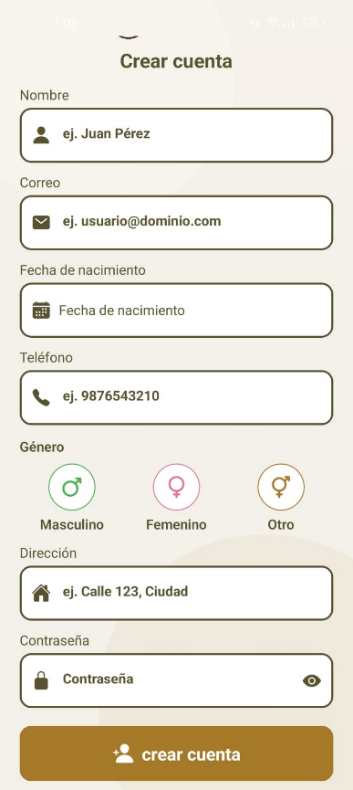
\includegraphics[width=0.35\textwidth]{images/image22.png}
					\end{figure}
					\tblnote
					
					\paragraph{Iniciar sesión.}
					Ingrese su correo electrónico y contraseña en la pantalla de inicio y presione \textbf{Iniciar sesión} (Figura~\ref{fig:man_login}). Si olvidó su contraseña, presione \textbf{¿Olvidaste tu contraseña?} para recuperarla por correo. Los niños no deben usar esta opción; su acceso se realiza exclusivamente a través del botón \textbf{Soy niño~--- Ingresar código}, descrito en la sección~\ref{ssec:modonino}.
					
					\begin{figure}[H]
						\caption{Interfaz de inicio de sesión}
						\label{fig:man_login}
						\centering
						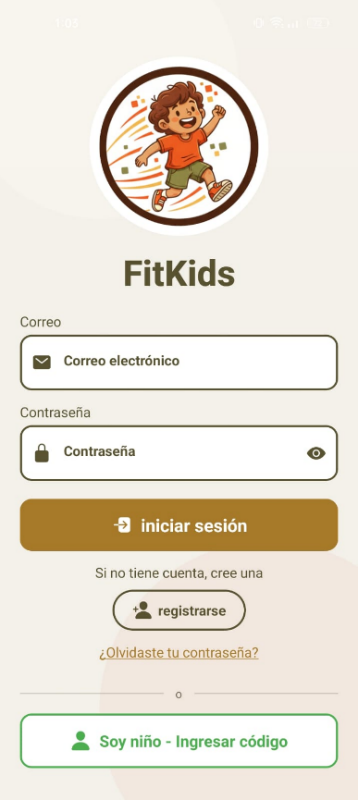
\includegraphics[width=0.35\textwidth]{images/image23.png}
					\end{figure}
					\tblnote
					
					\paragraph{Pantalla principal.}
					Tras iniciar sesión, el padre accede a la pantalla principal que muestra la Figura~\ref{fig:man_home}. En la barra superior se listan los perfiles de niños registrados; al seleccionar uno, el panel central actualiza su resumen diario: porcentaje de rutina completada, minutos activos del día y minutos activos acumulados en la semana. Desde esta pantalla se accede a las cuatro funciones principales: \textbf{Ver estadísticas}, \textbf{Configurar horarios} (recordatorios), \textbf{Agregar niño} y, en la barra inferior, \textbf{Configuración} y \textbf{Cerrar sesión}.
					
					\begin{figure}[H]
						\caption{Pantalla principal del perfil de padres}
						\label{fig:man_home}
						\centering
						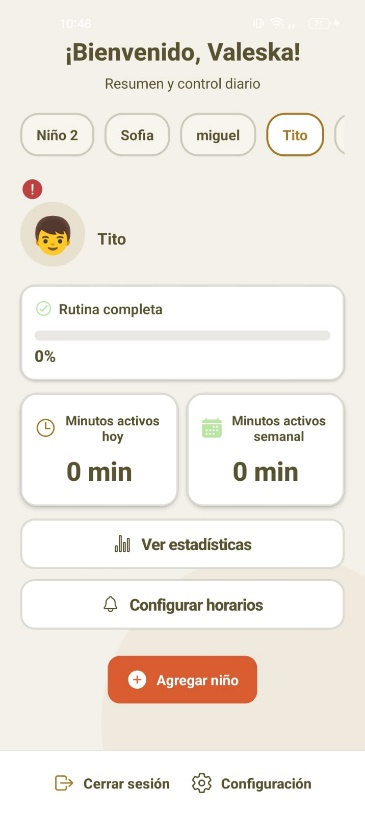
\includegraphics[width=0.35\textwidth]{images/image24.jpeg}
					\end{figure}
					\tblnote
					
					\paragraph{Registrar perfil del niño.}
					Presione \textbf{Agregar niño} en la pantalla principal. El sistema presenta un formulario de dos pasos. En el paso~1 (Figura~\ref{fig:man_registronino}, izquierda) complete: apodo, rango de edad, género, altura, peso y, de manera opcional, condiciones médicas o notas relevantes; luego presione \textbf{Continuar}. En el paso~2 (Figura~\ref{fig:man_registronino}, derecha) seleccione uno o más intereses deportivos del niño (por ejemplo, Atletismo, Fútbol, Baile) y presione \textbf{Guardar y finalizar}. Los datos de este perfil se utilizarán para personalizar todas las rutinas generadas por el sistema.
					
					\begin{figure}[H]
						\caption{Formulario de registro del niño: datos básicos (izquierda) e intereses deportivos (derecha)}
						\label{fig:man_registronino}
						\centering
						\begin{minipage}{0.42\textwidth}
							\centering
							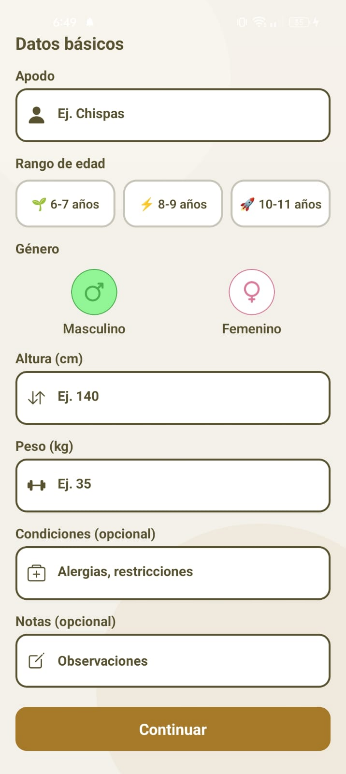
\includegraphics[width=\textwidth]{images/image26.png}
						\end{minipage}\hfill
						\begin{minipage}{0.42\textwidth}
							\centering
							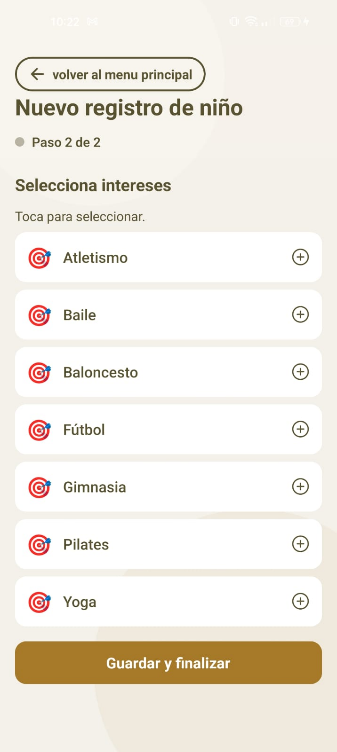
\includegraphics[width=\textwidth]{images/image25.png}
						\end{minipage}
					\end{figure}
					\tblnote
					
					\paragraph{Perfil del niño.}
					Para consultar o modificar los datos de un niño registrado, presione su apodo en la pantalla principal. La Figura~\ref{fig:man_perfil} muestra la pantalla de perfil, donde se visualizan el apodo, la fecha de nacimiento, el sexo, el peso, la estatura y las actividades preferidas. Para actualizar algún dato, presione \textbf{Modificar}, edite los campos necesarios y guarde los cambios. El sistema aplicará la información actualizada a las próximas rutinas generadas.
					
					\begin{figure}[H]
						\caption{Pantalla de perfil del niño}
						\label{fig:man_perfil}
						\centering
						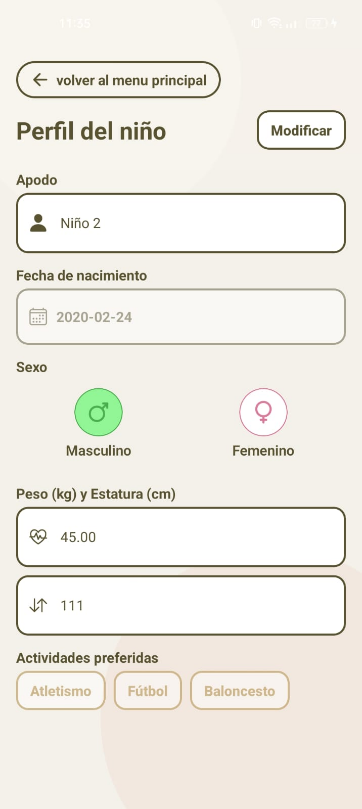
\includegraphics[width=0.35\textwidth]{images/image27.png}
					\end{figure}
					\tblnote
					
					\paragraph{Ver estadísticas de progreso.}
					Desde la pantalla principal, presione \textbf{Ver estadísticas}. Las Figuras~\ref{fig:man_stats1} y~\ref{fig:man_stats2} muestran la pantalla de estadísticas del niño seleccionado. El resumen de la semana indica los días completados, los minutos activos acumulados y el porcentaje de progreso semanal. El gráfico de barras diferencia visualmente los días cumplidos (verde), los incompletos (amarillo/ocre) y los no cumplidos (rojo). En la sección \textbf{Minutos activos} puede alternar entre las vistas Diaria, Semanal y Mensual. Para consultar el detalle día a día, presione \textbf{Mostrar detalle e historial} y seleccione cualquier fecha de la lista para ver los ejercicios realizados.
					
					\begin{figure}[H]
						\caption{Estadísticas semanales: resumen y gráfico de cumplimiento (izquierda) e historial y minutos activos (derecha)}
						\label{fig:man_stats1}
						\centering
						\begin{minipage}{0.42\textwidth}
							\centering
							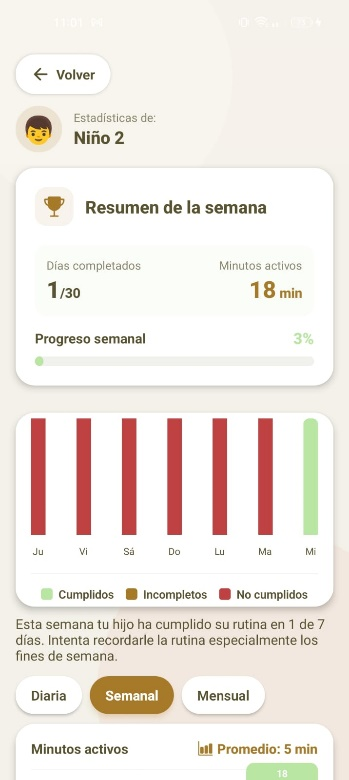
\includegraphics[width=\textwidth]{images/image30.jpeg}
						\end{minipage}\hfill
						\begin{minipage}{0.42\textwidth}
							\centering
							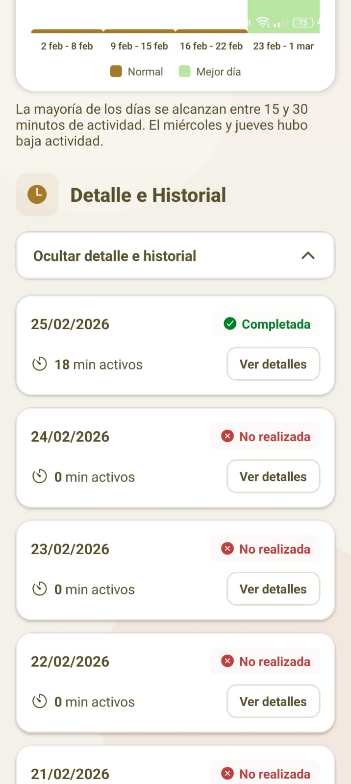
\includegraphics[width=\textwidth]{images/image28.png}
						\end{minipage}
					\end{figure}
					\tblnote
					
					\begin{figure}[H]
						\caption{Vista de detalle, historial de sesiones y análisis de minutos activos}
						\label{fig:man_stats2}
						\centering
						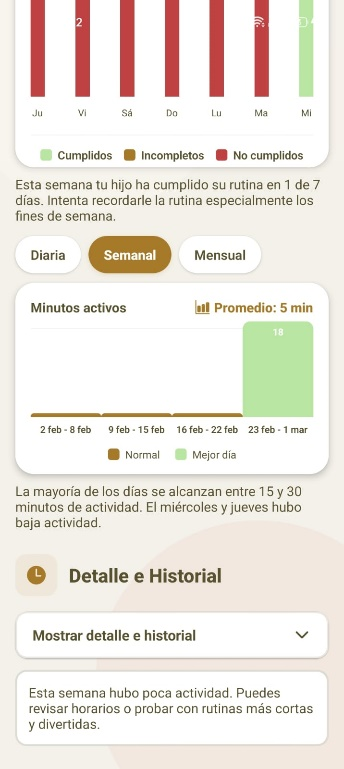
\includegraphics[width=0.35\textwidth]{images/image29.jpeg}
					\end{figure}
					\tblnote
					
					\paragraph{Configurar recordatorios.}
					Presione \textbf{Configurar horarios} en la pantalla principal. Como se aprecia en la Figura~\ref{fig:man_recordatorios}, la pantalla de recordatorios permite: activar o desactivar las notificaciones con el interruptor \textbf{ON/OFF}; seleccionar los días de la semana (D, L, M, X, J, V, S) en los que se enviará el recordatorio; elegir entre 1 o 2 recordatorios al día; y establecer la hora deseada. Cuando haya terminado, presione \textbf{Guardar configuración}. El sistema enviará una notificación push al dispositivo en el horario programado aunque la aplicación esté cerrada.
					
					\begin{figure}[H]
						\caption{Pantalla de configuración de recordatorios de actividad física}
						\label{fig:man_recordatorios}
						\centering
						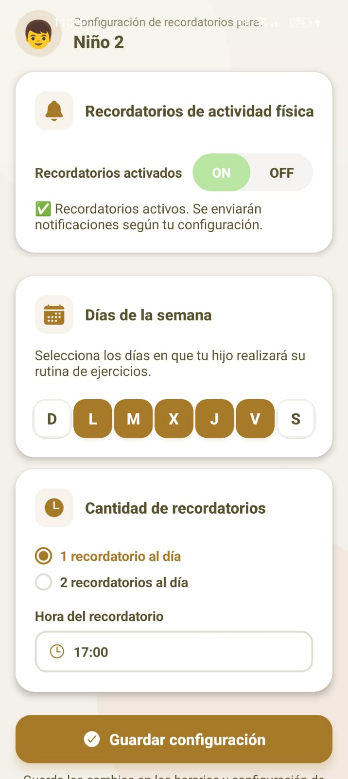
\includegraphics[width=0.35\textwidth]{images/image31}
					\end{figure}
					\tblnote
					
					\paragraph{Configuración general.}
					La sección Configuración (Figura~\ref{fig:man_config}) agrupa los ajustes personales del sistema. En \textbf{Mi Cuenta} puede consultar el correo registrado. En \textbf{Perfiles de Niños} visualiza los perfiles registrados y puede generar el código de acceso al modo niño (véase la sección~\ref{ssec:modonino}). En \textbf{Idioma} puede alternar entre Español e English. En \textbf{Tamaño de letra} elija entre Pequeña, Normal, Grande o Extra Grande; la vista previa refleja el cambio en tiempo real. La Figura~\ref{fig:man_voz} muestra la \textbf{Configuración de Voz}: seleccione la voz del asistente (Voz Hombre 1, Voz Hombre 2, Voz Mujer 1, Voz Mujer 2), ajuste el volumen (0--100\%) y la velocidad de lectura (0,5x--2,0x), y presione \textbf{Probar Voz} para escuchar una muestra antes de guardar. En \textbf{Tema de colores} (Figura~\ref{fig:man_colores}) seleccione el color de acento de la interfaz entre las seis opciones disponibles; la vista previa permite evaluar el contraste antes de confirmar la elección. Todos los cambios se aplican automáticamente al cerrar la pantalla.
					
					\begin{figure}[H]
						\caption{Pantalla de configuración general: cuenta, perfiles, idioma y tamaño de letra}
						\label{fig:man_config}
						\centering
						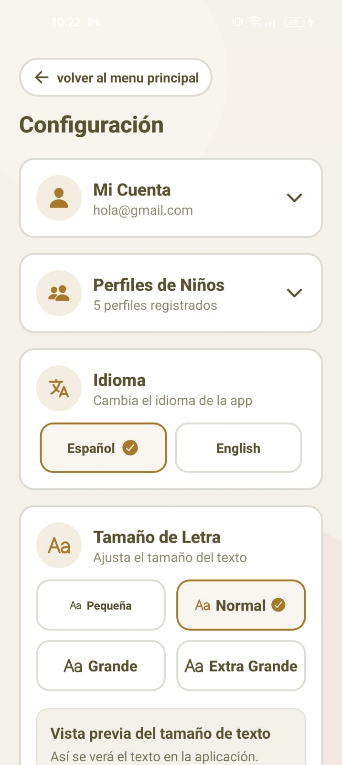
\includegraphics[width=0.35\textwidth]{images/image34.png}
					\end{figure}
					\tblnote
					
					\begin{figure}[H]
						\caption{Configuración de voz del asistente: tipo de voz, volumen y velocidad}
						\label{fig:man_voz}
						\centering
						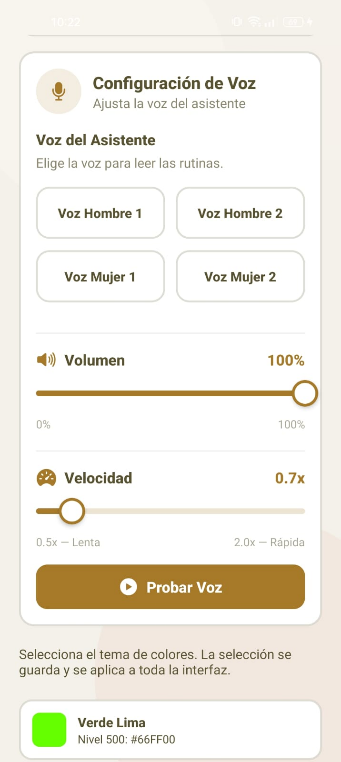
\includegraphics[width=0.35\textwidth]{images/image33.png}
					\end{figure}
					\tblnote
					
					\begin{figure}[H]
						\caption{Selector de tema de colores con vista previa de contraste}
						\label{fig:man_colores}
						\centering
						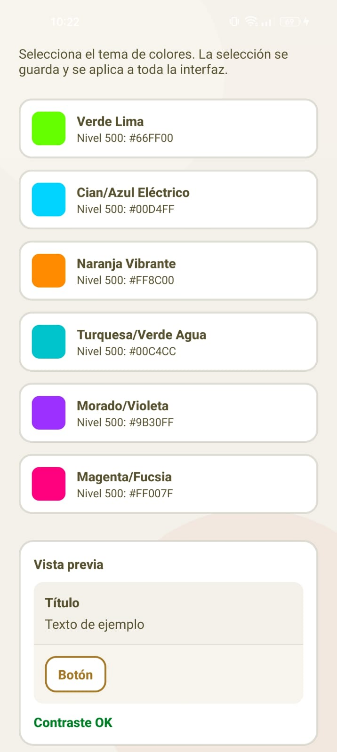
\includegraphics[width=0.35\textwidth]{images/image32.png}
					\end{figure}
					\tblnote
			
				\subsubsection{Modo niño}
					\label{ssec:modonino}
					
					El modo niño está diseñado para que el niño lo utilice de forma autónoma, con una interfaz simplificada, instrucciones por voz y elementos visuales adaptados a su rango etario. El acceso se realiza siempre mediante un código temporal generado por el padre, lo que garantiza que únicamente niños con perfil registrado puedan ingresar.
					
					\paragraph{Generar y usar el código de acceso.}
					Desde la pantalla principal del padre, ingrese a \textbf{Configuración} $\rightarrow$ \textbf{Perfiles de Niños}. Como muestra la Figura~\ref{fig:man_codigo} (izquierda), seleccione el perfil del niño y presione \textbf{Generar código de acceso}. Aparecerá una ventana con un código alfanumérico de 6 caracteres (Figura~\ref{fig:man_codigo}, derecha); puede copiarlo con el botón \textbf{Copiar código}. Entregue este código al niño. En el dispositivo del niño, en la pantalla de inicio de sesión, presione \textbf{Soy niño~--- Ingresar código} (Figura~\ref{fig:man_ingresonino}, izquierda); ingrese el código en los seis campos indicados y presione \textbf{¡Entrar a jugar!} (Figura~\ref{fig:man_ingresonino}, derecha). El código es de un solo uso: una vez utilizado queda invalidado automáticamente y será necesario generar uno nuevo para el siguiente acceso.
					
					\begin{figure}[H]
						\caption{Generación del código de acceso: lista de perfiles (izquierda) y ventana con el código (derecha)}
						\label{fig:man_codigo}
						\centering
						\begin{minipage}{0.42\textwidth}
							\centering
							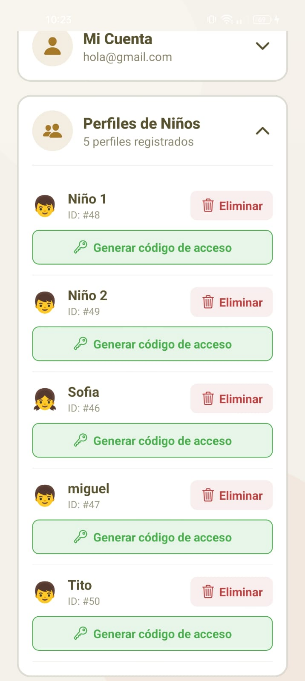
\includegraphics[width=\textwidth]{images/image35.png}
						\end{minipage}\hfill
						\begin{minipage}{0.42\textwidth}
							\centering
							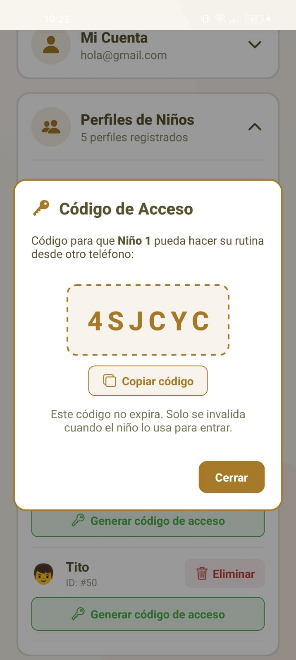
\includegraphics[width=\textwidth]{images/image36.png}
						\end{minipage}
					\end{figure}
					\tblnote
					
					\begin{figure}[H]
						\caption{Acceso al modo niño: botón de ingreso con código (izquierda) y pantalla de entrada del código (derecha)}
						\label{fig:man_ingresonino}
						\centering
						\begin{minipage}{0.42\textwidth}
							\centering
							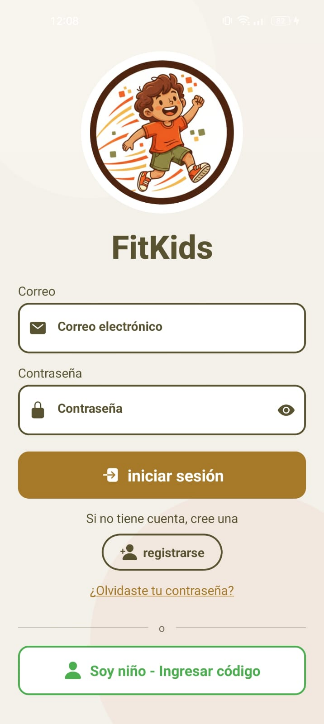
\includegraphics[width=\textwidth]{images/image37.png}
						\end{minipage}\hfill
						\begin{minipage}{0.42\textwidth}
							\centering
							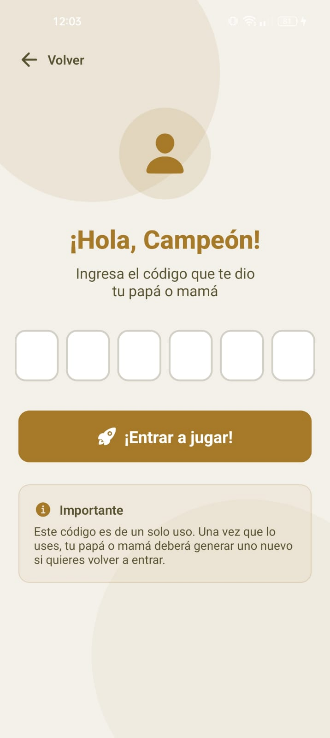
\includegraphics[width=\textwidth]{images/image38.png}
						\end{minipage}
					\end{figure}
					\tblnote
					
					\paragraph{Pantalla principal del modo niño.}
					Una vez validado el código, el niño accede a su pantalla de bienvenida (Figura~\ref{fig:man_kidmain}), que muestra su nombre, avatar, el porcentaje de avance de la rutina diaria, los minutos activos del día y de la semana, y un consejo motivacional. Para comenzar la sesión de ejercicios, el niño presiona el botón \textbf{¡JUGAR AHORA!}.
					
					\begin{figure}[H]
						\caption{Pantalla principal del modo niño}
						\label{fig:man_kidmain}
						\centering
						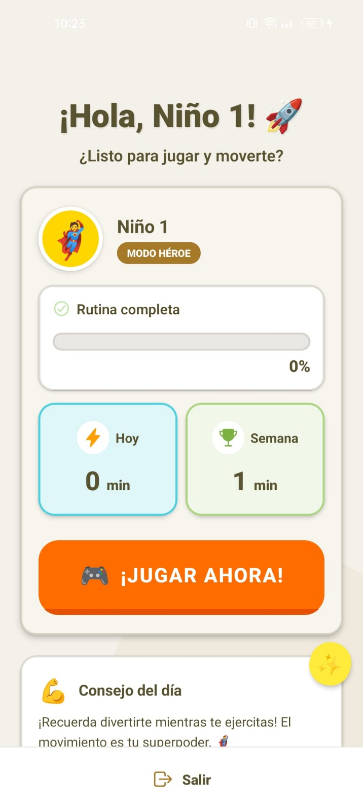
\includegraphics[width=0.35\textwidth]{images/image39.png}
					\end{figure}
					\tblnote
					
					\paragraph{Elegir la misión.}
					Al presionar \textbf{¡JUGAR AHORA!}, el sistema presenta la pantalla \textbf{¡Elige tu misión!} (Figura~\ref{fig:man_mision}, izquierda), donde el niño visualiza un mensaje motivacional y las tarjetas de actividad disponibles según sus intereses registrados. Al presionar \textbf{JUGAR}, el sistema genera la rutina del día y muestra la pantalla de preparación previa (Figura~\ref{fig:man_mision}, derecha), con recomendaciones ilustradas: hidratarse, usar ropa cómoda y escuchar al cuerpo. El niño presiona \textbf{¡Siguiente!} para iniciar los ejercicios.
					
					\begin{figure}[H]
						\caption{Selección de misión deportiva (izquierda) y preparación previa a la rutina (derecha)}
						\label{fig:man_mision}
						\centering
						\begin{minipage}{0.40\textwidth}
							\centering
							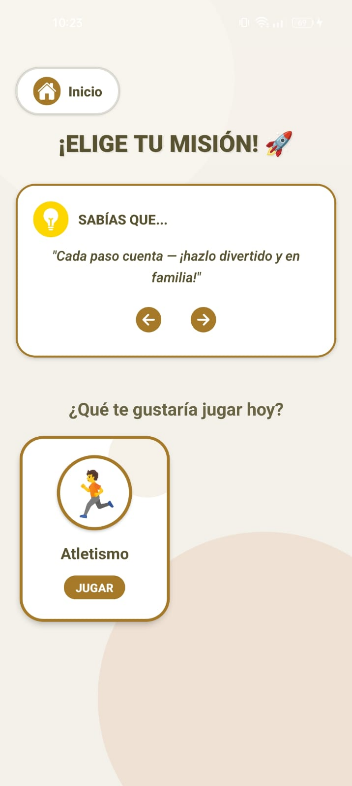
\includegraphics[width=\textwidth]{images/image40.png}
						\end{minipage}\hfill
						\begin{minipage}{0.40\textwidth}
							\centering
							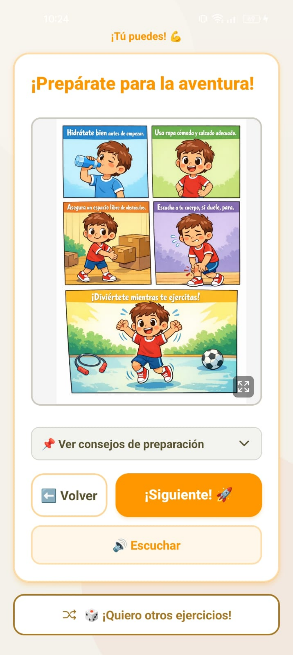
\includegraphics[width=\textwidth]{images/image41.png}
						\end{minipage}
					\end{figure}
					\tblnote
					
					\paragraph{Realización de la rutina.}
					La rutina se organiza en tres fases secuenciales ilustradas en la Figura~\ref{fig:man_fases}. En la \textbf{fase de preparación} (a la derecha en Figura~\ref{fig:man_mision}), el sistema presenta recomendaciones ilustradas antes de comenzar: hidratarse, usar ropa cómoda y escuchar al cuerpo; el niño presiona \textbf{¡Siguiente!} para avanzar. En la \textbf{fase de calentamiento} (Figura~\ref{fig:man_fases}, izquierda), la pantalla muestra el nombre del ejercicio, su número dentro de la secuencia, el tiempo transcurrido y las ilustraciones demostrativas del movimiento; el niño puede presionar \textbf{Ver instrucciones} para leer los pasos o \textbf{Escuchar} para activar el lector de voz, y al terminar cada ejercicio presiona \textbf{¡Siguiente!} para continuar o \textbf{Volver} si necesita repetirlo. En la \textbf{fase de ejercicios principales} (Figura~\ref{fig:man_fases}, centro), cuando el niño considera que completó el movimiento presiona \textbf{¡Ejercicio completado!} para que el sistema registre el tiempo activo y avance automáticamente al siguiente. En la \textbf{fase de estiramiento} (Figura~\ref{fig:man_fases}, derecha), el niño presiona \textbf{¡Lo logré!} al finalizar cada movimiento. En cualquier momento puede presionar \textbf{¡Quiero otros ejercicios!} en la barra inferior para que el sistema genere una rutina alternativa. Al completar las tres fases, el sistema muestra la pantalla de felicitación con confeti y el mensaje \textbf{¡FELICIDADES! ¡Has completado tu rutina!} (Figura~\ref{fig:man_fin}), y registra la sesión automáticamente en el historial del niño.
					
					\begin{figure}[H]
						\caption{Fases de la rutina de ejercicios: calentamiento (izquierda), ejercicios principales (centro) y estiramiento (derecha)}
						\label{fig:man_fases}
						\centering
						\begin{minipage}{0.31\textwidth}
							\centering
							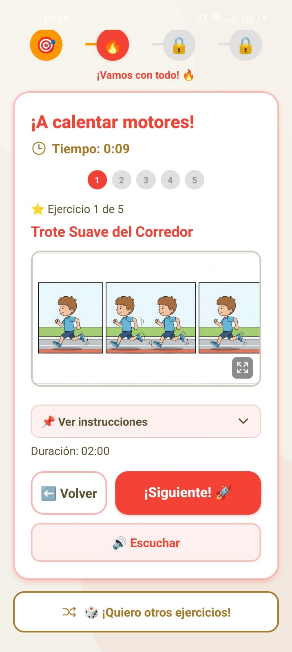
\includegraphics[width=\textwidth]{images/image43.png}
						\end{minipage}\hfill
						\begin{minipage}{0.31\textwidth}
							\centering
							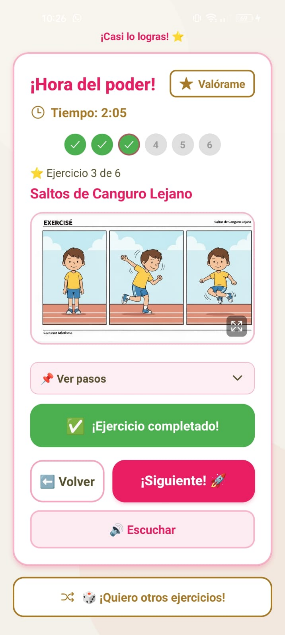
\includegraphics[width=\textwidth]{images/image42.png}
						\end{minipage}\hfill
						\begin{minipage}{0.31\textwidth}
							\centering
							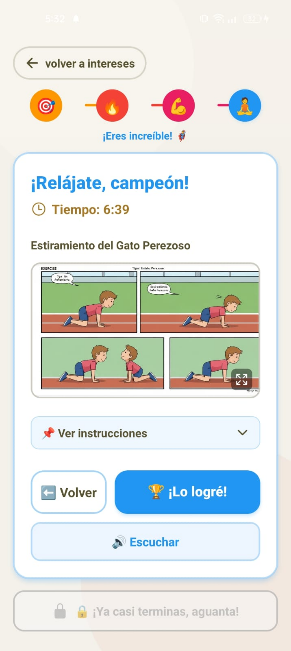
\includegraphics[width=\textwidth]{images/image44.png}
						\end{minipage}
					\end{figure}
					\tblnote
					
					\begin{figure}[H]
						\caption{Pantalla de felicitación al completar la rutina diaria}
						\label{fig:man_fin}
						\centering
						
\includegraphics[width=0.35\textwidth]{images/image45.png}
					\end{figure}
					\tblnote
					
				\subsubsection{Aplicación web para especialistas}
				\label{sec:appwebesp}
					La aplicación web es el entorno exclusivo del especialista (pediatra). Desde aquí se gestionan los ejercicios que conforman el catálogo disponible para la generación de rutinas en la app móvil. El acceso requiere una cuenta de tipo especialista registrada previamente.
					
					\paragraph{Inicio de sesión.}
					Ingrese a la URL de la aplicación web desde cualquier navegador. En la pantalla de inicio (Figura~\ref{fig:man_weblogin}), escriba su correo electrónico y contraseña y presione \textbf{Iniciar sesión}.
					
					\begin{figure}[H]
						\caption{Pantalla de inicio de sesión del módulo web para especialistas}
						\label{fig:man_weblogin}
						\centering
						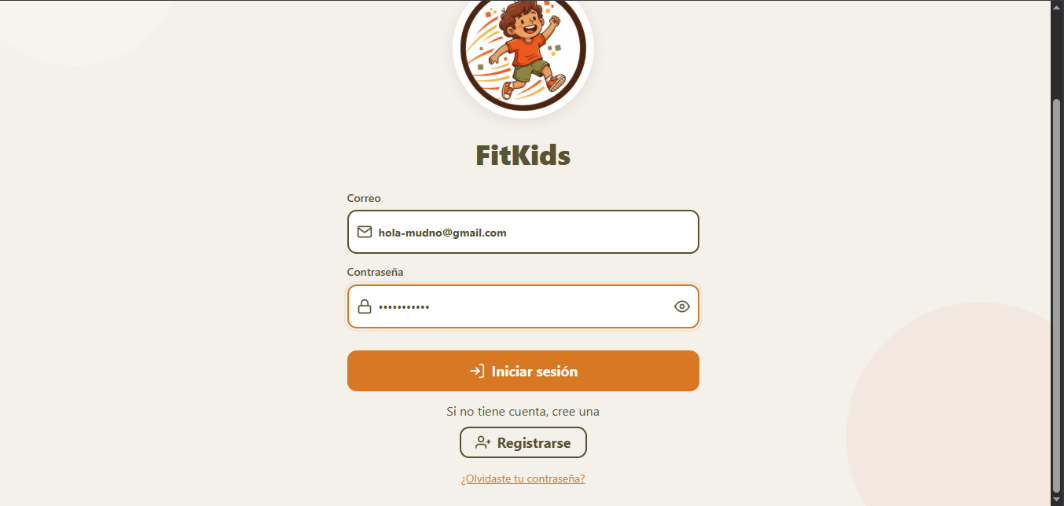
\includegraphics[width=0.85\textwidth]{images/image46.png}
					\end{figure}
					\tblnote
					
					\paragraph{Generador de ejercicios.}
					La Figura~\ref{fig:man_webgen} muestra el Generador de Ejercicios. Seleccione uno o más intereses deportivos de la lista (Atletismo, Baile, Baloncesto, Fútbol, Gimnasia, Pilates, Yoga), elija el rango de edad objetivo (6--7, 8--9 o 10--11 años) y presione \textbf{Generar Ejercicios}. El sistema enviará la solicitud al modelo de IA y, en algunos segundos, presentará las tarjetas de ejercicios generados en estado ``Pendiente de revisión''.
					
					\begin{figure}[H]
						\caption{Generador de ejercicios: selección de intereses y rango de edad}
						\label{fig:man_webgen}
						\centering
						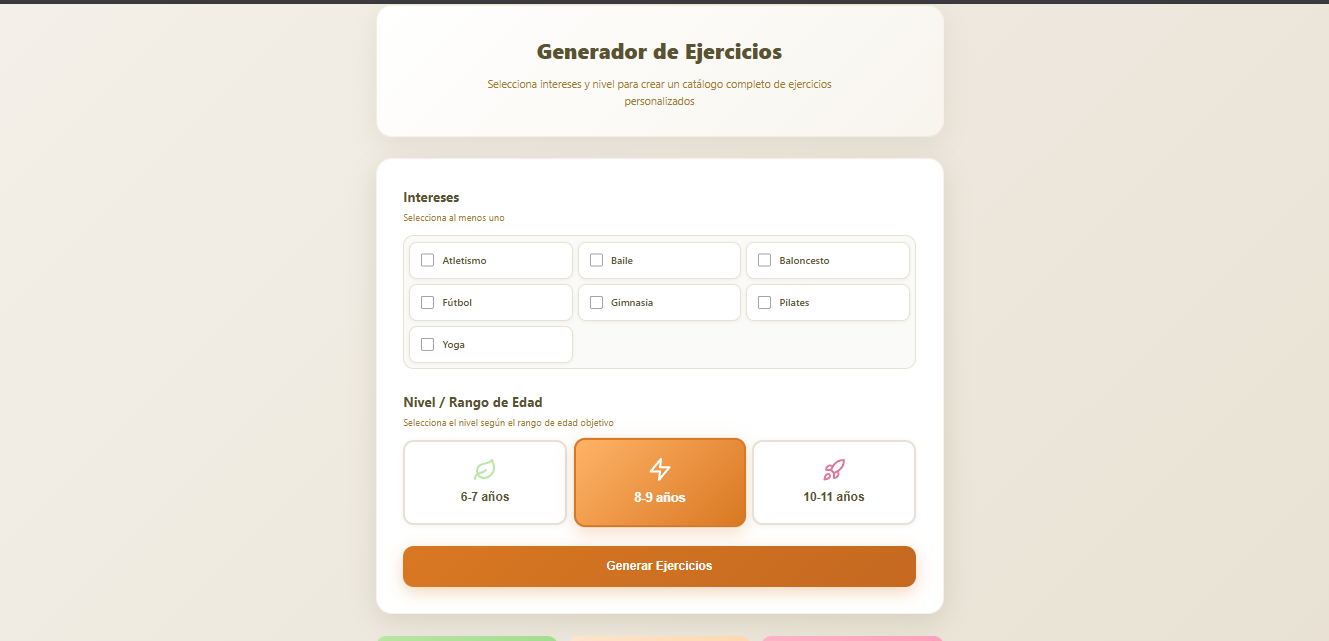
\includegraphics[width=0.85\textwidth]{images/image47.png}
					\end{figure}
					\tblnote
					
					\paragraph{Revisión y aprobación de ejercicios.}
					En la pantalla de revisión (Figura~\ref{fig:man_webrev}) cada tarjeta muestra el nombre del ejercicio, su categoría (calentamiento, principal o estiramiento), la descripción y los pasos. Para cada ejercicio, presione \textbf{Aprobar} o \textbf{Rechazar} individualmente, o use los botones \textbf{Aprobar Todos} y \textbf{Rechazar Todos} para procesar el lote completo. Solo los ejercicios aprobados podrán recibir imágenes y ser publicados al catálogo.
					
					\begin{figure}[H]
						\caption{Pantalla de revisión y aprobación de ejercicios generados por IA}
						\label{fig:man_webrev}
						\centering
						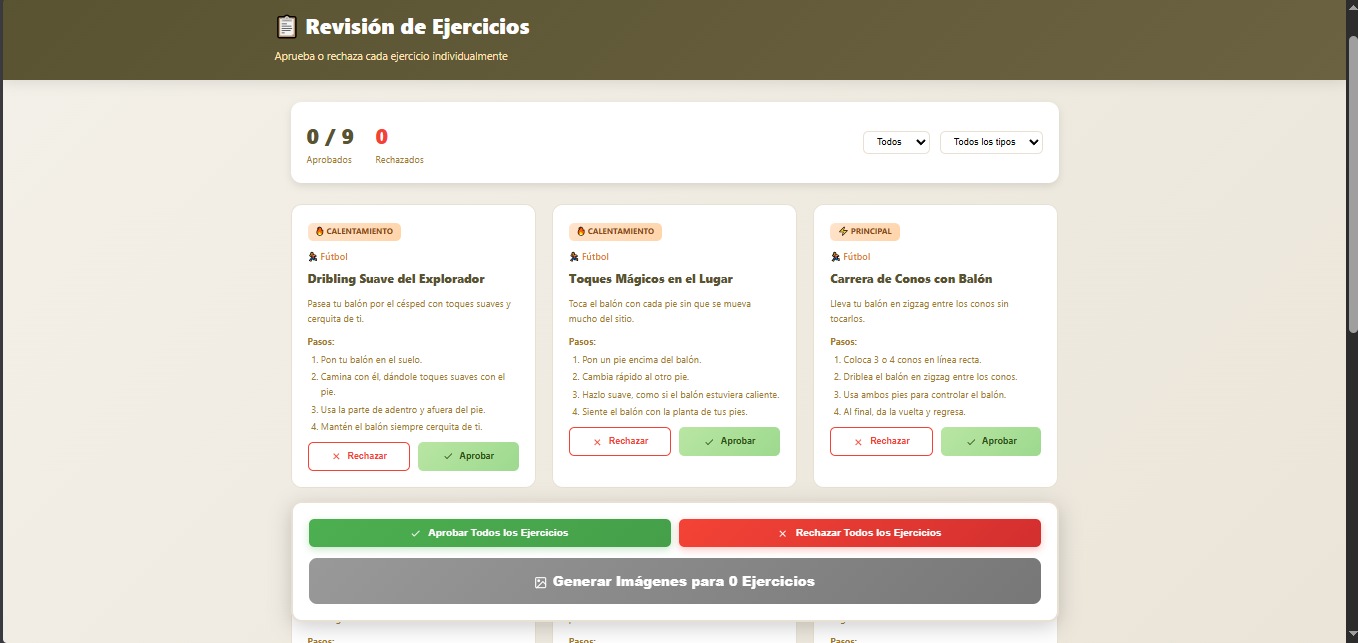
\includegraphics[width=0.85\textwidth]{images/image48.png}
					\end{figure}
					\tblnote
					
					\paragraph{Generación y aprobación de imágenes.}
					Una vez aprobados los ejercicios, presione \textbf{Generar Imágenes para \textit{N} Ejercicios}. El sistema creará ilustraciones en estilo cómic infantil para cada ejercicio aprobado. Cuando el proceso concluya, aparecerá la confirmación que muestra la Figura~\ref{fig:man_webimg}. Revise las imágenes generadas: presione \textbf{Aprobar Todas las Imágenes} si son satisfactorias, o \textbf{Marcar Todas como Pendientes} para regenerarlas. Una vez aprobadas las imágenes, presione \textbf{Publicar \textit{N} Ejercicios con Imágenes} para que los ejercicios pasen al catálogo activo y queden disponibles para la generación de rutinas en la aplicación móvil.
					
					\begin{figure}[H]
						\caption{Confirmación de imágenes generadas y opciones de publicación}
						\label{fig:man_webimg}
						\centering
						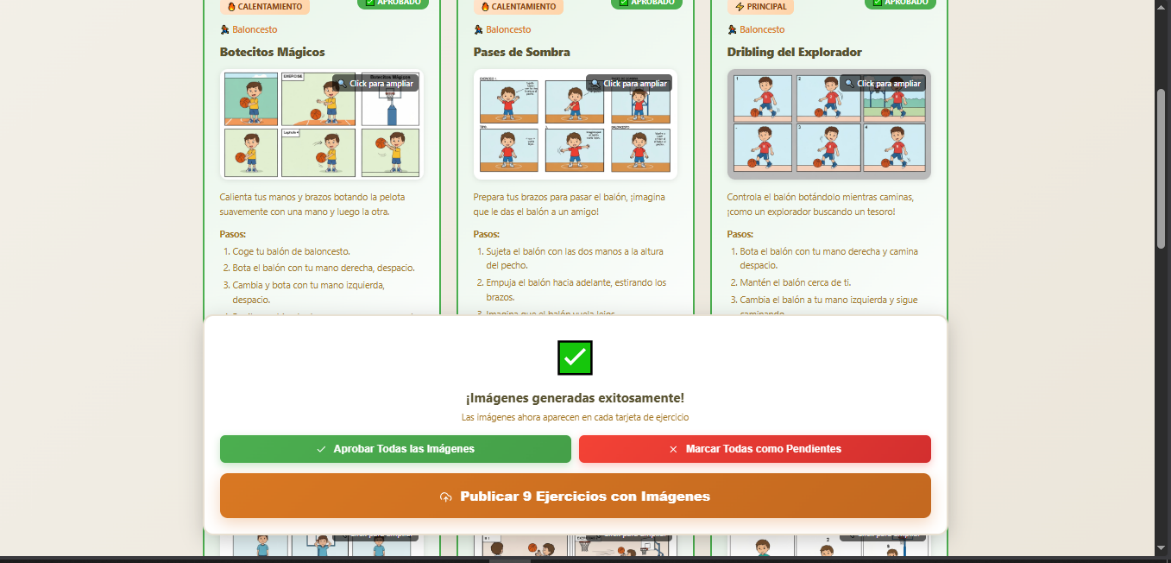
\includegraphics[width=0.85\textwidth]{images/image49.png}
					\end{figure}
					\tblnote
					
					\paragraph{Gestión de intereses.}
					El panel de gestión de intereses (Figura~\ref{fig:man_webint}) muestra el total de intereses registrados y cuántos están activos o inactivos. Desde aquí puede crear un nuevo interés presionando \textbf{+ Nuevo interés}, editar el nombre de uno existente, activarlo o desactivarlo sin eliminarlo, o eliminarlo definitivamente. Los intereses activos son los que aparecen disponibles tanto en el Generador de Ejercicios como en el formulario de registro del perfil del niño en la app móvil.
					
					\begin{figure}[H]
						\caption{Panel de gestión de intereses deportivos disponibles en el sistema}
						\label{fig:man_webint}
						\centering
						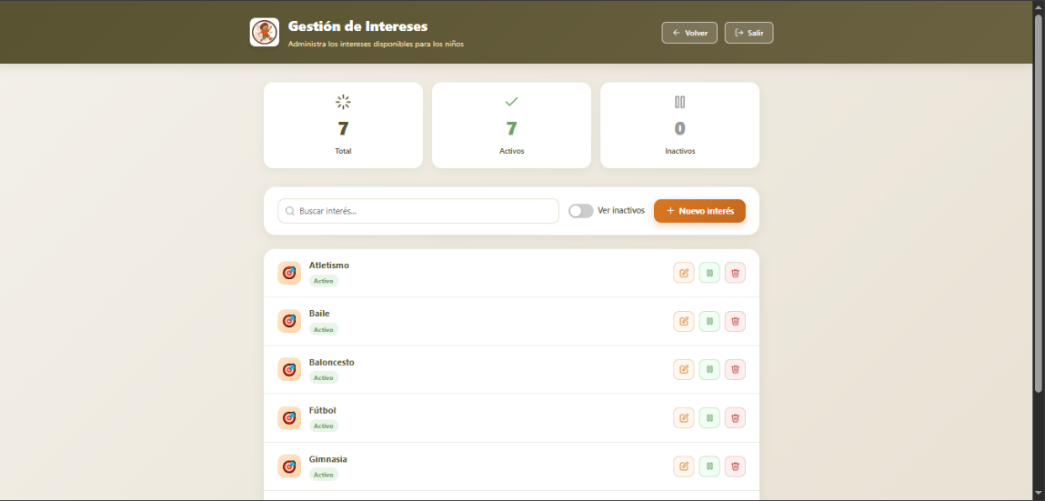
\includegraphics[width=0.85\textwidth]{images/image50.png}
					\end{figure}
					\tblnote
					
					\paragraph{Panel de reportes.}
					La Figura~\ref{fig:man_webrep} muestra el panel de reportes, que presenta estadísticas generales del sistema en tiempo real: número de niños registrados, intereses activos, total de ejercicios en el catálogo e intereses asignados con al menos un niño. El panel incluye además el \textit{ranking} de intereses (más y menos popular), la distribución de niños por género, el número de ejercicios por categoría deportiva y el estado general del catálogo de intereses.
					
					\begin{figure}[H]
						\caption{Panel de reportes del módulo web: estadísticas generales del sistema}
						\label{fig:man_webrep}
						\centering
						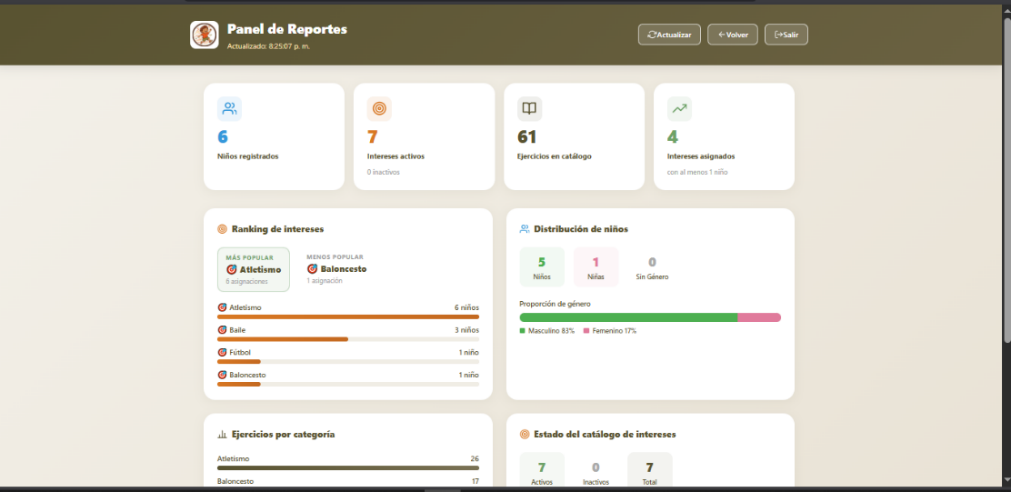
\includegraphics[width=0.85\textwidth]{images/image51.png}
					\end{figure}
					\tblnote

		\section{Conclusiones}
		\label{sec:conclu}
			FitKids integra, en un único sistema, tres atributos que la literatura previa había abordado de manera aislada: personalización dinámica mediante inteligencia artificial generativa, validación profesional obligatoria pre-publicación y supervisión parental estructural con capacidades de monitoreo y configuración. Ninguno de los trabajos revisados ---MiniMovers~\cite{Zhang2024}, KIJANI~\cite{Willinger2024}, Sworkit Kids~\cite{Papastergiou2021}, las intervenciones de seguimiento de pasos~\cite{GomezCuesta2024,MateoOrcajada2024} ni los estudios de prescripción por LLM~\cite{Zaleski2026,Dergaa2024}--- combina estos tres atributos simultáneamente, lo que sitúa a FitKids en un espacio conceptual no cubierto por la literatura especializada en aplicaciones mHealth para infancia.
			
			La revisión sistemática de literatura y las entrevistas a especialistas y padres confirmaron que la personalización por edad y condición física, el acompañamiento parental y los elementos motivacionales son los ejes críticos que la evidencia científica asocia con la adherencia infantil a la actividad física~\cite{Yao2015,VegaDiaz2023}. Esta triangulación orientó directamente las decisiones de diseño funcional del sistema y explica la convergencia entre las dimensiones TAM observada en la evaluación: los padres valoran por igual la utilidad del sistema y la facilidad con que pueden operar sus funciones de supervisión, resultado escasamente reportado en aplicaciones comparables~\cite{Venkatesh2003}.
			
			La solución técnica construida sobre una arquitectura distribuida de cuatro capas alcanzó el 100\% de cobertura de pruebas sobre los 44~casos definidos y el 100\% de cumplimiento sobre los 16~requisitos formalizados, valores que superan los umbrales de aceptación establecidos y se ubican dentro de los estándares ISO/IEC~25010~\cite{GuerreroUlloa2024}. Los tiempos de respuesta medidos ---480~ms en autenticación, 320~ms en consulta de progreso y 1~850~ms en generación de rutinas--- confirman que el sistema opera con eficiencia aceptable incluso en la operación que involucra un servicio externo de IA, donde la latencia depende de factores fuera del control del sistema.
			
			La tasa de aprobación del 84\% sobre los 50~ejercicios generados por el modelo Gemini demuestra la viabilidad técnica del enfoque de generación parametrizada por perfil infantil. El 16\% de rechazos ---por intensidad excesiva, instrucciones poco claras o riesgo de lesión--- no representa una debilidad del modelo sino la confirmación de que el filtro humano funciona como fue diseñado: ningún ejercicio clínicamente inadecuado llegó al niño usuario. Este hallazgo aporta evidencia inicial específica para población infantil en un dominio que Zaleski et al.~\cite{Zaleski2026} y Dergaa et al.~\cite{Dergaa2024} habían explorado exclusivamente sobre población adulta o clínica.
			
			La evaluación con usuarios arrojó un puntaje SUS de 81,17~puntos ---categoría ``excelente'' según Bangor et al.~\cite{Bangor2008} y 13~puntos por encima de la media normativa global~\cite{Lewis2018}--- y medias TAM de 4,37 en utilidad percibida y 4,25 en facilidad de uso, ambas superiores al umbral de aceptación de Davis~\cite{Davis1989}. Estos valores son superiores o comparables a los reportados por KIJANI~\cite{Willinger2024}, MiniMovers~\cite{Zhang2024} y Gómez-Cuesta et al.~\cite{GomezCuesta2024}, y destacan por la simetría entre dimensiones TAM, patrón que la literatura sobre adherencia parental identifica como indicador de sostenibilidad de uso~\cite{VegaDiaz2023,Yao2015}. La evaluación cualitativa de las dos especialistas pediatras refuerza la coherencia de estos resultados: la valoración positiva sobre la calidad clínica del contenido es consistente con la tasa de aprobación del 84\% y con la ausencia de objecciones críticas de seguridad.
			
			La adherencia promedio del 68\% y el incremento de 0,7~puntos en el PAQ-C~\cite{Kowalski2004,Benitez2016} durante las cuatro semanas de observación ofrecen evidencia inicial de impacto conductual, superior en frecuencia semanal a la reportada por Domin et al.~\cite{Domin2022} y coherente con los ensayos de Gómez-Cuesta et al.~\cite{GomezCuesta2024}. El subgrupo de baja adherencia (27\%) confirma lo documentado en los meta-análisis sobre intervenciones mHealth pediátricas~\cite{Schoeppe2017}: la disponibilidad tecnológica no garantiza por sí sola el cambio conductual sostenido, y el acompañamiento parental activo ---precisamente el eje que diferencia a FitKids de las propuestas con supervisión baja o nula~\cite{Papastergiou2021,MateoOrcajada2024}--- es la condición necesaria para sostener la práctica en el tiempo.
			
			Como prototipo funcional con arquitectura escalable y plan de mantenimiento documentado, FitKids demuestra que la combinación de IA generativa, validación clínica profesional y supervisión parental integrada es una vía técnicamente viable y aceptable para promover la actividad física infantil en el contexto doméstico, respondiendo directamente a las recomendaciones de la OMS sobre los 60~minutos diarios de actividad moderada a vigorosa en menores de 5 a 17~años~\cite{Bull2020}.


		\section{Recomendaciones}
		\label{sec:recomend}
			Las recomendaciones se organizan en cuatro dimensiones: metodológica, técnica, clínica y de inclusión.
			
			Desde la \textbf{perspectiva metodológica}, se recomienda ampliar el tamaño muestral e incorporar diseños cuasi-experimentales o experimentales con seguimiento longitudinal de al menos 12~semanas y grupos de control, lo que permitiría establecer relaciones causales entre el uso de FitKids y la mejora sostenida de la actividad física infantil~\cite{GomezCuesta2024,Schoeppe2017}. Aunque el tamaño muestral adoptado ($n = 15$ por perfil) es apropiado para la fase formativa de evaluación de software~\cite{Putnam2020}, estudios futuros con muestras superiores a 30~participantes podrían incorporar pruebas estadísticas no paramétricas ---como Mann-Whitney o Wilcoxon--- para contrastar diferencias entre subgrupos etarios o niveles de adherencia~\cite{HernandezSampieri2014}. Complementariamente, la integración de acelerometría permitiría contrastar los registros de tiempo activo del sistema con mediciones objetivas independientes, en línea con las prácticas adoptadas por Domin et al.~\cite{Domin2022} y Mateo-Orcajada et al.~\cite{MateoOrcajada2024}. Se recomienda asimismo incorporar una evaluación heurística formal con al menos tres especialistas en usabilidad infantil~\cite{Nielsen1994}, que aportaría perspectivas complementarias a los resultados obtenidos mediante el cuestionario SUS aplicado directamente con los usuarios.
			
			Desde la \textbf{dimensión técnica}, se recomienda ampliar la cobertura del sistema mediante el desarrollo de versiones compatibles con iOS o de una aplicación web progresiva, lo que reduciría las barreras de acceso asociadas al sistema operativo y ampliaría el número de familias beneficiadas~\cite{Pressman2020}. Igualmente, conviene fortalecer la reproducibilidad del sistema mediante la publicación del código fuente en un repositorio accesible con versiones de dependencias explícitas y documentación completa del modelo de datos, prácticas alineadas con los principios de ingeniería de software abierta~\cite{Fowler2002,Pressman2020}.
			
			Desde la \textbf{dimensión clínica e IA generativa}, se recomienda desarrollar evaluaciones sistemáticas que comparen formalmente la calidad de las rutinas generadas por el modelo Gemini con planes diseñados directamente por profesionales de la salud, utilizando criterios clínicos y pedagógicos alineados con las guías internacionales de actividad física infantil~\cite{Zaleski2026,Dergaa2024}. Explorar el ajuste fino del modelo sobre corpus específicos de ejercicio físico pediátrico reduciría la tasa de rechazos por intensidad excesiva o inadecuación clínica, y la integración de interfaces conversacionales permitiría a los padres interactuar de forma más natural con el sistema~\cite{Yim2024,Sengar2024}.
			
			Desde la \textbf{dimensión de inclusión y adherencia}, se recomienda incorporar mecanismos de gamificación complementarios al eje de validación profesional ---en la línea de lo implementado por KIJANI~\cite{Willinger2024}---, siempre que estén diseñados de modo que el entretenimiento no comprometa el rigor clínico del contenido. Finalmente, ampliar la cobertura geográfica mediante estudios multicéntricos que consideren distintos contextos socioeconómicos del Ecuador y de la región latinoamericana permitiría atender las variables contextuales ---espacio en el hogar, seguridad del entorno, disponibilidad de dispositivos--- documentadas por Hesketh et al.~\cite{VegaDiaz2023} como determinantes de la adherencia en intervenciones digitales para población infantil~\cite{Bull2020}.


	
	% ============================================================
	% BIBLIOGRAFÍA
	% ============================================================
	\clearpage
	\addcontentsline{toc}{chapter}{Bibliografía}
	\bibliography{referencias}
	
	% ============================================================
	% ANEXOS
	% ============================================================
	% ============================================================
% ANEXOS
% ============================================================
\clearpage
\appendix
\chapter{ANEXOS}
\addcontentsline{toc}{chapter}{Anexos}

	\section[Entrevistas a representantes legales]{Consentimiento informado de los padres para entrevista.}
		CONSENTIMIENTO INFORMADO PARA EL REGISTRO COMO PARTICIPANTE
		
		Yo, \_\_\_\_\_\_\_\_\_\_\_\_\_\_\_\_\_\_\_\_\_\_\_\_\_\_\_\_\_\_\_\_\_\_\_\_\_\_\_\_\_\_\_\_\_\_\_\_\_\_\_\_\_\_\_\_\_\_\_, portador(a) de la cédula de ciudadanía N.° \_\_\_\_\_\_\_\_\_\_\_\_\_\_\_\_\_\_\_\_\_\_\_\_\_\_, en calidad de padre, madre o representante legal del niño(a) \_\_\_\_\_\_\_\_\_\_\_\_\_\_\_\_\_\_\_\_\_\_\_\_\_\_\_\_\_\_\_\_\_\_\_\_\_\_\_, de \_\_\_\_\_\_ años de edad, declaro que he sido informado(a) de manera clara y suficiente sobre el proyecto de titulación titulado ``Aplicación móvil con inteligencia artificial generativa para crear planes de ejercicios físicos personalizados para niños'', desarrollado en la Carrera de Ingeniería de Software de la Universidad Técnica Estatal de Quevedo.
		
		Se me ha explicado que mi participación consistirá en una entrevista semiestructurada en la que se me consultará acerca de los hábitos de actividad física de mi hijo(a), las dificultades y motivaciones que se presentan en el entorno familiar, así como mi opinión sobre el uso de aplicaciones móviles como apoyo para fomentar hábitos saludables en la infancia.
		
		Comprendo que:
		
		- Mi participación es voluntaria y puedo retirarme en cualquier momento, sin que esto implique perjuicio alguno para mí ni para mi hijo(a).
		
		- La entrevista será grabada en audio exclusivamente para fines académicos, con el propósito de facilitar la transcripción y el análisis de la información, manteniendo en todo momento la confidencialidad de nuestra identidad.
		
		- La información que proporcione será utilizada solo con fines académicos, resguardando nuestra identidad mediante el uso de códigos o seudónimos.
		
		- Los datos obtenidos serán tratados con confidencialidad, de acuerdo con las políticas de la institución.
		
		Habiendo comprendido la información anterior y aclarado mis dudas, ACEPTO PARTICIPAR de forma libre y voluntaria en este estudio.
		
		Lugar y fecha: \_\_\_\_\_\_\_\_\_\_\_\_\_\_\_\_\_\_\_\_\_\_\_\_\_\_\_\_\_\_\_\_\_\_\_\_\_\_\_\_\_\_\_\_\_\_\_\_\_\_\_\_\_\_\_\_\_\_
		
		\vspace{24pt}
		Firma del participante como representante legal: \_\_\_\_\_\_\_\_\_\_\_\_\_\_\_\_\_\_\_\_\_\_\_\_\_\_\_\_\_\_\_\_
		
		Nombre completo: \_\_\_\_\_\_\_\_\_\_\_\_\_\_\_\_\_\_\_\_\_\_\_\_\_\_\_\_\_\_\_\_\_\_\_\_\_\_\_\_\_\_\_\_\_\_\_\_\_\_\_\_\_\_\_
	
	\section[Entrevistas a especializas de la actividad física]{Consentimiento informado a especialistas en actividad física infantil para entrevista.}
		
		CONSENTIMIENTO INFORMADO PARA EL REGISTRO COMO PARTICIPANTE
		
		Yo, \_\_\_\_\_\_\_\_\_\_\_\_\_\_\_\_\_\_\_\_\_\_\_\_\_\_\_\_\_\_\_\_\_\_\_\_\_\_\_\_\_\_\_\_\_\_\_\_\_\_\_\_\_\_\_\_\_\_\_, portador(a) de la cédula de ciudadanía No. \_\_\_\_\_\_\_\_\_\_\_\_\_\_\_\_\_\_\_\_\, declaro que he sido informado(a) de manera clara y suficiente sobre el proyecto de titulación titulado ``Aplicación móvil con inteligencia artificial generativa para crear planes de ejercicios físicos personalizados para niños'', desarrollado en la Carrera de Ingeniería de Software de la Universidad Técnica Estatal de Quevedo.
		
		Se me ha explicado que mi participación consistirá en una entrevista semiestructurada en la que se me consultará, en calidad de especialista de niños, sobre mis criterios profesionales en relación con la actividad física en niños, los riesgos y precauciones a considerar, así como mi opinión sobre el uso de aplicaciones móviles como apoyo para fomentar hábitos saludables en la infancia.
		
		Comprendo que:
		
		- Mi participación es voluntaria y puedo retirarme en cualquier momento, sin que esto implique perjuicio alguno.
		
		- La entrevista será grabada en audio exclusivamente para fines académicos, con el propósito de facilitar la transcripción y el análisis de la información, manteniendo en todo momento la confidencialidad de mi identidad.
		
		- La información que proporcione será utilizada solo con fines académicos, resguardando mi identidad mediante el uso de códigos o seudónimos.
		
		- Los datos obtenidos serán tratados con confidencialidad, de acuerdo con las políticas de la institución.
		
		Habiendo comprendido la información anterior y aclarado mis dudas, ACEPTO PARTICIPAR de forma libre y voluntaria en este estudio.
		
		Lugar y fecha: \_\_\_\_\_\_\_\_\_\_\_\_\_\_\_\_\_\_\_\_\_\_\_\_\_\_\_\_\_\_\_\_\_\_\_\_\_\_\_\_\_\_\_\_\_\_\_\_
		
		\vspace{24pt}
		Firma del participante: \_\_\_\_\_\_\_\_\_\_\_\_\_\_\_\_\_\_\_\_\_\_\_\_\_\_\_\_\_\_\_\_\_\_\_\_\_\_\_\_\_\_
		
		Nombre completo: \_\_\_\_\_\_\_\_\_\_\_\_\_\_\_\_\_\_\_\_\_\_\_\_\_\_\_\_\_\_\_\_\_\_\_\_\_\_\_\_\_\_\_\_\_
		
	\section[Padres participantes en la evaluación]{Consentimiento informado para padres o representantes legales de niños participantes}
		\label{app:conrepnino}
		CONSENTIMIENTO INFORMADO PARA PADRES, MADRES O REPRESENTANTES LEGALES
		
		Proyecto de Titulación: Proyecto Tecnológico
		
		Título del Proyecto: Aplicación móvil con inteligencia artificial generativa para crear planes de ejercicios físicos personalizados para niños
		
		Autora: Valeska Sofía Chica Valfre
		
		Director: PhD. Gleiston Cicerón Guerrero Ulloa
		
		Datos del representante legal
		
		Nombre: \_\_\_\_\_\_\_\_\_\_\_\_\_\_\_\_\_\_\_\_\_\_\_\_\_\_\_\_\_\_\_\_\_\_\_\_\_\_\_\_\_\_\_\_\_\_
		
		Cédula: \_\_\_\_\_\_\_\_\_\_\_\_\_\_\_\_\_\_\_\_\_\_\_\_\_\_\_\_\_\_\_\_\_\_\_\_\_\_\_\_\_\_\_\_\_\_
		
		Correo electrónico: \_\_\_\_\_\_\_\_\_\_\_\_\_\_\_\_\_\_\_\_\_\_\_\_\_\_\_\_\_\_\_\_\_\_\_
		
		En cumplimiento de la Ley Orgánica de Protección de Datos Personales (Registro Oficial Suplemento No. 459, 26 de mayo de 2021), yo, en calidad de padre, madre o representante legal, autorizo de manera libre, voluntaria, expresa e informada la participación del niño, niña o representado bajo mi tutela en el proyecto tecnológico indicado, así como la captura y uso de imágenes (fotografías y/o videos) y el tratamiento de datos personales relacionados con su participación, exclusivamente con fines académicos, científicos, investigativos y administrativos.
		
		Las imágenes y datos personales serán utilizados únicamente para evidenciar el desarrollo, validación y resultados del proyecto en la Carrera de Ingeniería de Software de la Facultad de Ciencias de la Computación y Diseño Digital de la Universidad Técnica Estatal de Quevedo (UTEQ), así como para informes académicos, documentos de titulación, presentaciones y procesos de evaluación institucional. No se autoriza su uso con fines comerciales, publicitarios o de lucro.
		
		Declaro haber sido informado/a de mis derechos de acceso, rectificación, actualización, eliminación, revocación del consentimiento en cualquier momento, negativa sin perjuicio alguno, gratuidad y recepción de una copia del presente documento. Asimismo, libero de responsabilidad civil, administrativa o legal a la UTEQ y a los miembros vinculados al proyecto, siempre que el uso de la información se realice conforme a los fines aquí descritos.
		
		Manifiesto que he leído y comprendido el contenido de este consentimiento, que mis dudas han sido aclaradas y que otorgo esta autorización de forma libre y consciente, velando por el interés superior del niño, niña o representado.
		
		Firma del padre, madre o representante legal: \_\_\_\_\_\_\_\_\_\_\_\_\_\_\_\_\_\_\_\_\_\_\_\_\_
		
		Valeska Sofía Chica Valfre: \_\_\_\_\_\_\_\_\_\_\_\_\_\_\_\_\_\_\_\_
		
		Firma del director del proyecto: \_\_\_\_\_\_\_\_\_\_\_\_\_\_\_\_\_\_\_
		
	\section[Especialistas participantes en la evaluación]{Consentimiento informado para especialistas participantes en la evaluación del sistema}
		CONSENTIMIENTO INFORMADO PARA ESPECIALISTAS
		
		Proyecto de Titulación: Proyecto Tecnológico
		
		Título del Proyecto:
		
		Aplicación móvil con inteligencia artificial generativa para crear planes de ejercicios físicos personalizados para niños
		
		Autora: Valeska Sofía Chica Valfre
		
		Director: PhD. Gleiston Cicerón Guerrero Ulloa
		
		Datos del especialista participante
		
		Nombre: \_\_\_\_\_\_\_\_\_\_\_\_\_\_\_\_\_\_\_\_\_\_\_\_\_\_\_\_\_\_\_\_\_\_\_\_\_\_\_\_\_\_\_\_\_\_
		
		Cédula: \_\_\_\_\_\_\_\_\_\_\_\_\_\_\_\_\_\_\_\_\_\_\_\_\_\_\_\_\_\_\_\_\_\_\_\_\_\_\_\_\_\_\_\_\_\_
		
		Correo electrónico: \_\_\_\_\_\_\_\_\_\_\_\_\_\_\_\_\_\_\_\_\_\_\_\_\_\_\_\_\_\_\_\_\_\_\_
		
		En cumplimiento de la Ley Orgánica de Protección de Datos Personales (Registro Oficial Suplemento No. 459, 26 de mayo de 2021), yo, en calidad de especialista participante, autorizo de manera libre, voluntaria, expresa e informada mi participación en el proyecto tecnológico indicado, específicamente en la prueba y validación de la aplicación web administrativa del sistema.
		
		Autorizo el tratamiento de mis datos personales básicos (nombre, correo electrónico, profesión y respuestas obtenidas en evaluaciones de usabilidad o aceptación tecnológica), exclusivamente con fines académicos, científicos, investigativos y administrativos relacionados con el desarrollo, validación y evaluación del sistema.
		
		La información recopilada será utilizada únicamente para evidenciar el funcionamiento, análisis de resultados, pruebas de integración y evaluación del sistema dentro de la Carrera de Ingeniería de Software de la Facultad de Ciencias de la Computación y Diseño Digital de la Universidad Técnica Estatal de Quevedo (UTEQ), así como para informes académicos, documentos de titulación, presentaciones y procesos de evaluación institucional. No se autoriza su uso con fines comerciales, publicitarios o de lucro.
		
		Declaro haber sido informado/a de mis derechos de acceso, rectificación, actualización, eliminación, revocación del consentimiento en cualquier momento, negativa sin perjuicio alguno, gratuidad y recepción de una copia del presente documento. Asimismo, exonero de responsabilidad civil, administrativa o legal a la UTEQ y a los miembros vinculados al proyecto, siempre que el uso de la información se realice conforme a los fines aquí descritos.
		
		Manifiesto que he leído y comprendido el contenido de este consentimiento, que mis dudas han sido aclaradas y que otorgo esta autorización de forma libre y consciente.
		
		Firma del especialista: \_\_\_\_\_\_\_\_\_\_\_\_\_\_\_\_\_\_\_\_\_\_\_\_\_
		
		Valeska Sofía Chica Valfre: \_\_\_\_\_\_\_\_\_\_\_\_\_\_\_\_\_\_\_\_
		
		Firma del director del proyecto: \_\_\_\_\_\_\_\_\_\_\_\_\_\_\_\_\_\_\_
	\section{Guion de entrevista semiestructurada de padres.}
		1. Tiempo activo vs pantallas
		
		En un día típico, ¿cuánto tiempo aproximadamente pasa su hijo/a realizando actividad física y cuánto tiempo frente a pantallas (celular, tablet, TV, videojuegos)?
		
		2. Actividades favoritas
		
		¿Qué actividades físicas le gusta más hacer a su hijo/a (jugar al aire libre, deportes, bailar, etc.)?
		
		3. Barreras
		
		¿Qué dificultades o barreras encuentra para que su hijo/a realice más actividad física (falta de tiempo, espacios, seguridad, desinterés, tareas, etc.)?
		
		4. Motivación
		
		¿Qué cosas suelen motivar más a su hijo/a a levantarse y moverse (jugar con amigos, retos, premios, participación de la familia, música, etc.)?
		
		5. Efecto del ejercicio
		
		¿Ha notado cambios en el estado de ánimo o comportamiento de su hijo/a cuando realiza más actividad física (más alegre, duerme mejor, más tranquilo, etc.)?
		
		6. Monitoreo actual
		
		¿Cómo suele saber o controlar si su hijo/a está haciendo suficiente actividad física (horarios, comentarios de la escuela, observación directa, etc.)?
		
		7. Información deseada
		
		¿Qué tipo de información le gustaría recibir sobre el progreso de su hijo/a (minutos de ejercicio, tipo de actividades, logros alcanzados, alertas si no cumple, etc.)?
		
		8. Experiencia con apps
		
		¿Ha usado alguna aplicación relacionada con salud o ejercicio para usted o su hijo/a? ¿Cómo fue esa experiencia?
		
		9. Interés y características de una app
		
		Si existiera una aplicación que generara rutinas personalizadas de ejercicio para su hijo/a, ¿la usaría? ¿Qué características le parecerían más importantes (juegos, recompensas, videos explicativos, panel para padres, etc.)?
		
		10. Preocupaciones y ``app ideal''
		
		¿Qué le preocupa del uso de aplicaciones por parte de los niños (tiempo de pantalla, privacidad, contenido) y qué le pediría a una ``app ideal'' que ayude a que los niños hagan más ejercicio?
		
	\section{Guion de entrevista semiestructurada de especialistas}
	\label{app:guion_enter}
		1.	Situación actual y causas
		
		Desde su experiencia en consulta, ¿cómo describiría el nivel de actividad física de los niños de 6 a 11 años que atiende habitualmente? ¿Qué factores considera que contribuyen más al sedentarismo (uso de pantallas, entorno familiar, escuela, alimentación, etc.)?
		
		2.	Consecuencias clínicas
		
		En su práctica, ¿qué consecuencias observa con mayor frecuencia asociadas a la falta de actividad física en esta población (sobrepeso/obesidad, problemas posturales, trastornos del sueño, estado de ánimo, rendimiento escolar, etc.)?
		
		3.	Recomendaciones y seguridad
		
		De forma general, ¿qué tipo de actividades físicas suele recomendar a niños de 6 a 11 años y con qué frecuencia y duración? Desde el punto de vista pediátrico, ¿qué aspectos considera imprescindibles para que estas rutinas sean seguras (evaluaciones previas, antecedentes médicos, signos de alarma, intensidad, progresión, etc.)?
		
		4.	Personalización y adherencia
		
		¿Qué factores clínicos y personales considera clave para personalizar las recomendaciones de actividad física (IMC, comorbilidades, desarrollo psicomotor, gustos del niño, contexto familiar, diagnóstico previo, etc.) y qué estrategias o elementos ayudan más a que los niños sigan de manera constante dichas recomendaciones (juego, metas, participación de la familia, recompensas, trabajo con la escuela, etc.)?
		
		5.	Apps e inteligencia artificial
		
		¿Qué opinión le merece el uso de aplicaciones móviles ---incluyendo herramientas con inteligencia artificial--- como apoyo para fomentar la actividad física en niños? En su criterio, ¿qué funcionalidades y tipos de datos deberían incluirse o evitarse para que una aplicación que genere rutinas de ejercicio personalizadas sea útil y segura (registro de tiempo activo, alertas, validación médica, límites de intensidad, mensajes de advertencia, protección de datos, etc.)?

	\section{Cuestionario SUS}
	
	\section{Cuestionario TAM (UP)}
	
	\section{Cuestionario TAM (FUP)}
	
	\section{Preguntas cualitativas para la evaluación del sistema web}
		Preguntas cualitativas para la evaluación del sistema web (especialistas)
		
		¿Cómo describiría su experiencia general al utilizar el sistema web para la revisión y validación de ejercicios?
		
		¿El flujo de trabajo para revisar y aprobar ejercicios le resultó claro y comprensible?
		
		¿La información presentada por el sistema es suficiente para tomar decisiones sobre la aprobación de los ejercicios?
		
		¿Qué opinión le merece la calidad de los ejercicios generados por la inteligencia artificial?
		
		¿Las imágenes asociadas a los ejercicios facilitan la comprensión de las actividades propuestas?
		
		Desde su experiencia profesional, ¿considera que los ejercicios son adecuados y seguros para la población infantil?
		
		¿Encontró dificultades al navegar o utilizar alguna funcionalidad del sistema web?
		
		¿El sistema le genera confianza como herramienta de apoyo profesional para la validación de ejercicios?
		
		¿Qué aspectos del sistema web considera que deberían mejorarse?
		
		¿Recomendaría el uso de este sistema en un contexto profesional? ¿Por qué?

	\section{Evidencias de las actividades con los participantes}
		\subsection{Los niños probando la aplicación}
			\begin{figure}[H]
				\centering
				\caption{Realizando pruebas con los niños}
				\begin{minipage}{0.45\textwidth}
					\centering
					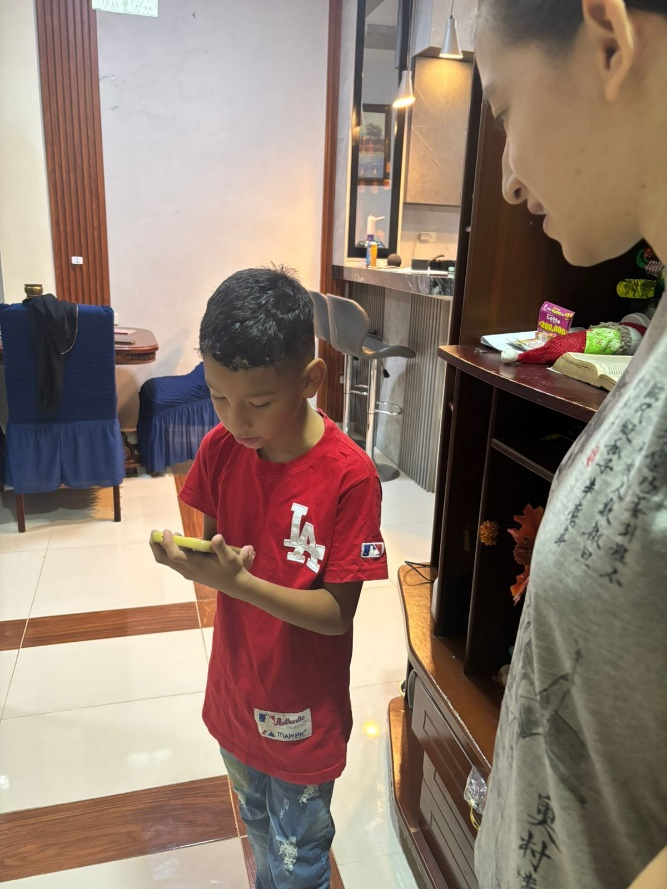
\includegraphics[width=\textwidth]{images/image52.jpeg}
				\end{minipage}\hfill
				\begin{minipage}{0.45\textwidth}
					\centering
					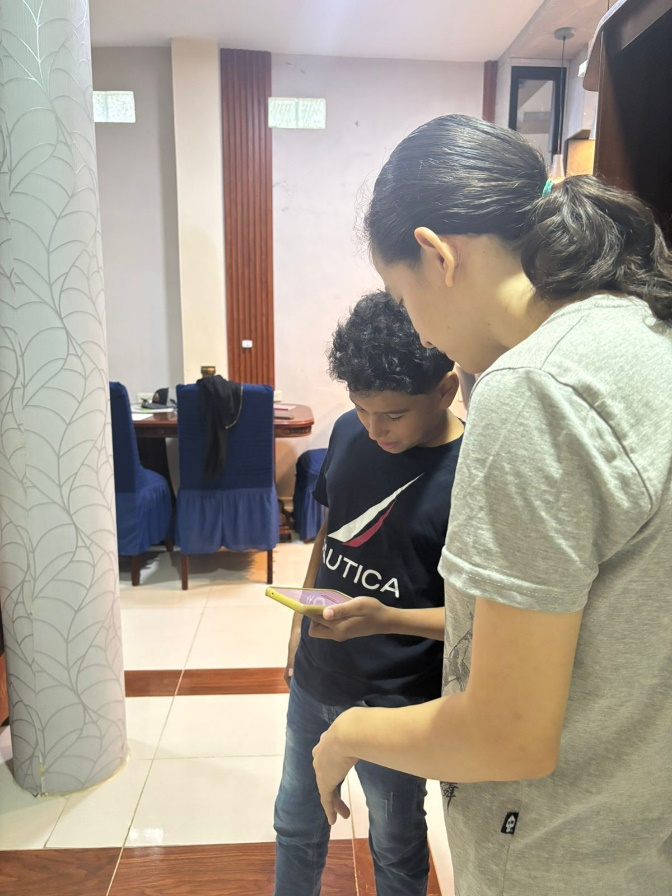
\includegraphics[width=\textwidth]{images/image53.jpeg}
				\end{minipage}\hfill \vspace{6pt}
				\begin{minipage}{0.45\textwidth}\centering
					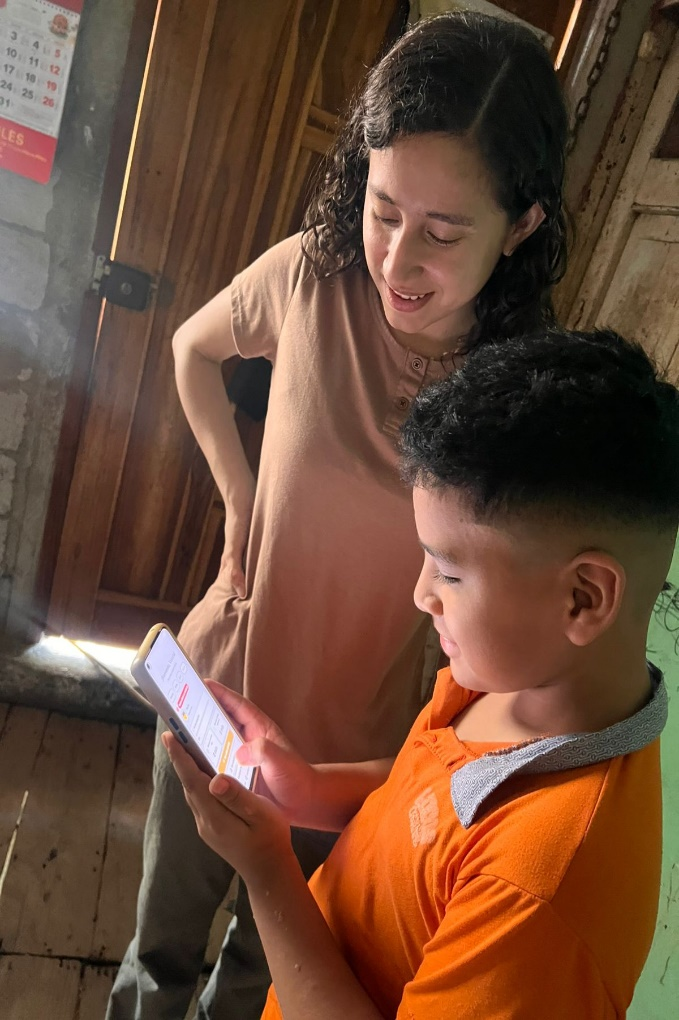
\includegraphics[width=\textwidth]{images/image54.jpeg}
				\end{minipage}\hfill
				\begin{minipage}{0.45\textwidth}\centering
					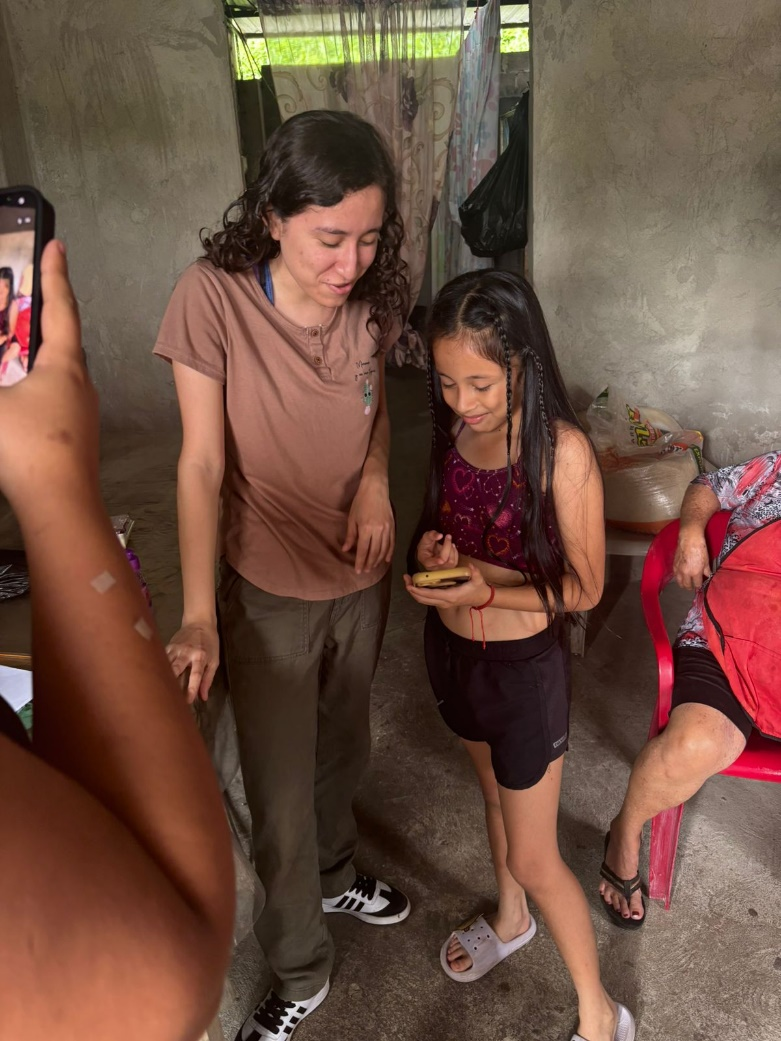
\includegraphics[width=\textwidth]{images/image55.jpeg}
				\end{minipage}\hfill
			\end{figure}
		
		\subsection{Los representantes usando la aplicación}
			\begin{figure}[H]
				\centering
				\caption{Realizando pruebas con los representantes}
				\begin{minipage}{0.45\textwidth}\centering
					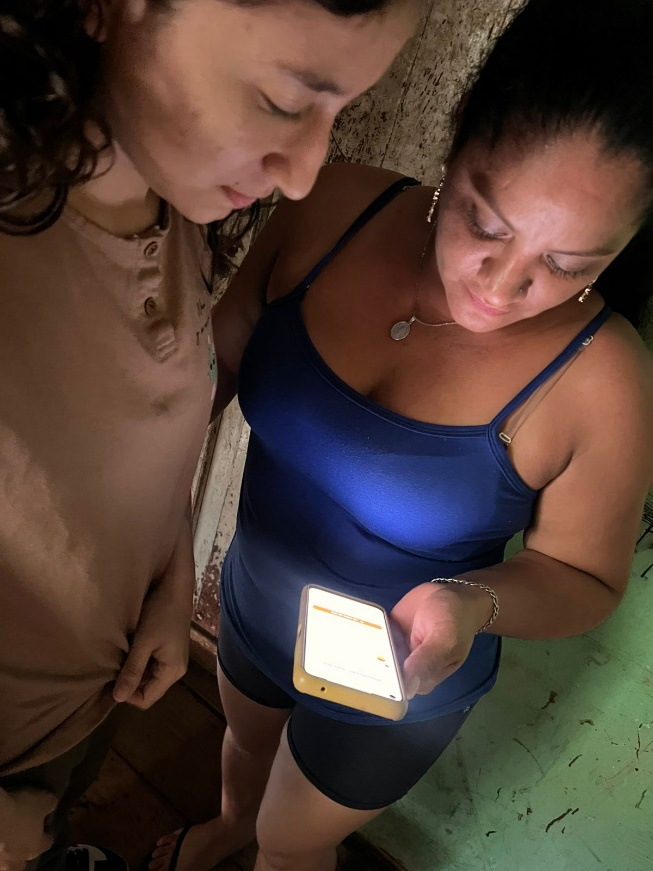
\includegraphics[width=\textwidth]{images/image56.jpeg}
				\end{minipage}\hfill
				\begin{minipage}{0.45\textwidth}\centering
					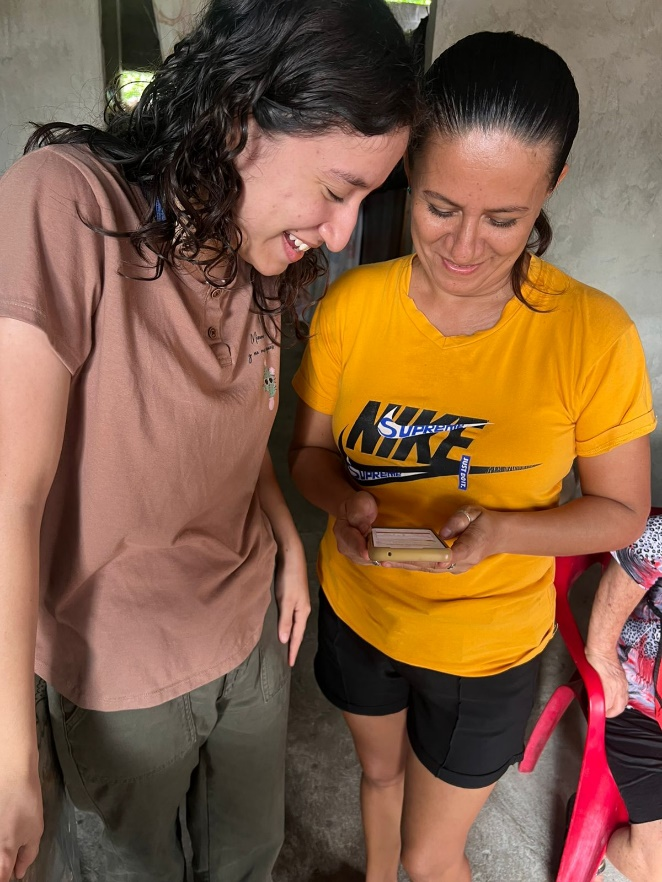
\includegraphics[width=\textwidth]{images/image57.jpeg}
				\end{minipage}\hfill
			\end{figure}
		
		\subsection{Los especialistas usando la aplicación}
			\begin{figure}[H]
				\centering
				\caption{El especialista probando la aplicación}
				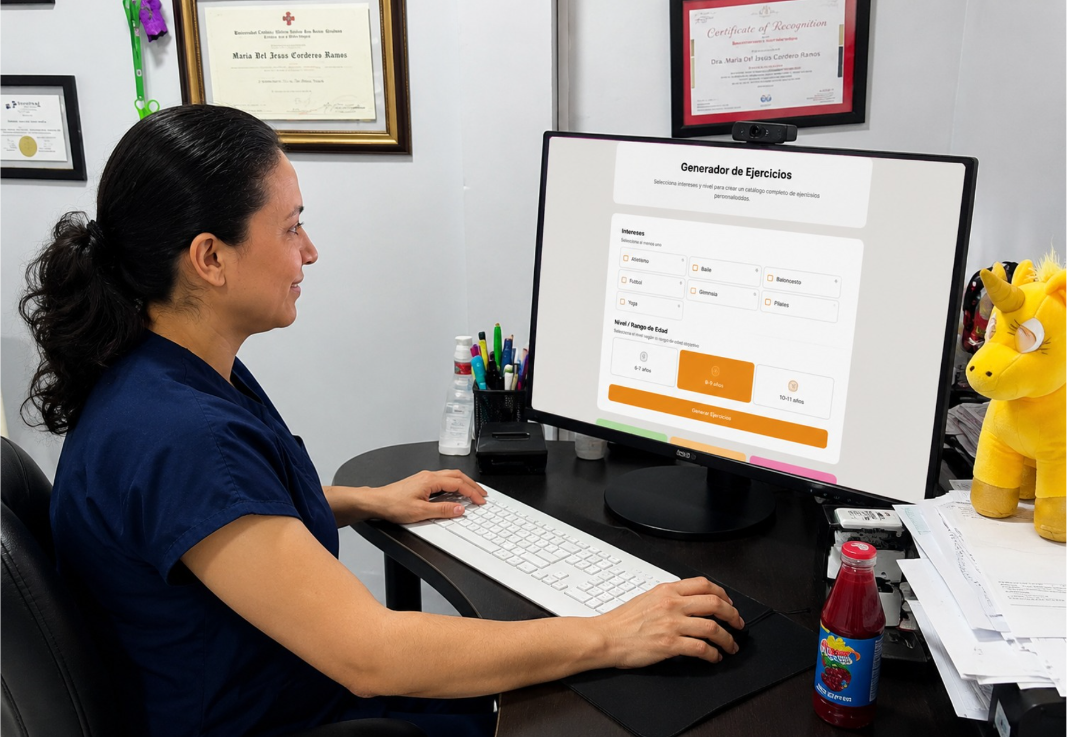
\includegraphics[width=0.8\textwidth]{images/image58.png}
			\end{figure}
			
			\begin{figure}[H]
				\centering
				\caption{Evaluando la aplicación}
				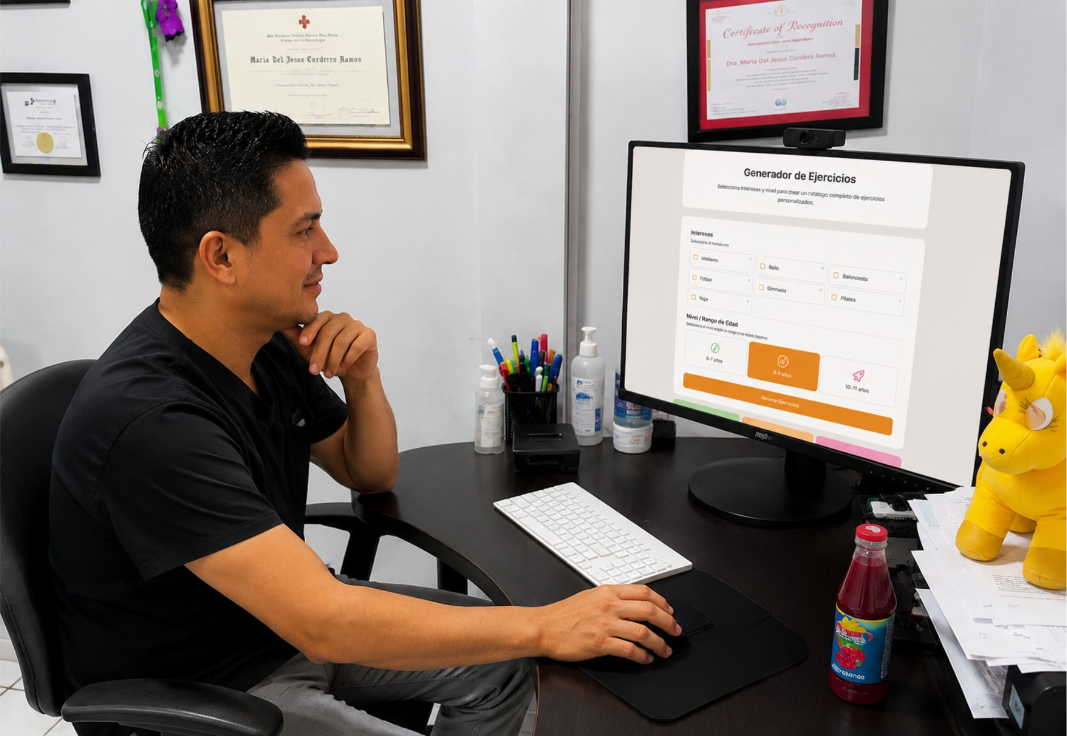
\includegraphics[width=0.8\textwidth]{images/image59.png}
			\end{figure}
			
		\section{Aplicando los cuestionario de evaluación de FitKids}
			\begin{figure}[H]
				\centering
				\caption{Especialista rellenando el cuestionario SUS}
				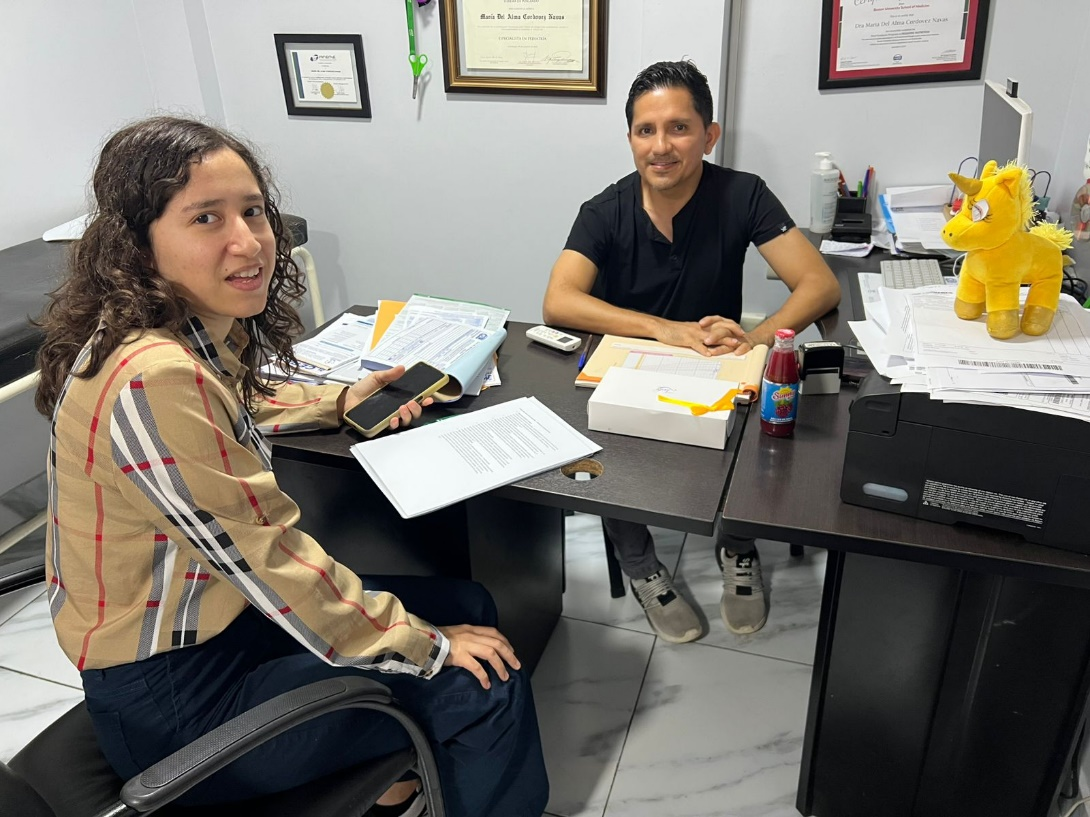
\includegraphics[width=0.8\textwidth]{images/image60.png}
			\end{figure}
			
			\begin{figure}[H]
				\centering
				\caption{Especialista rellenando el cuestionario TAM}
				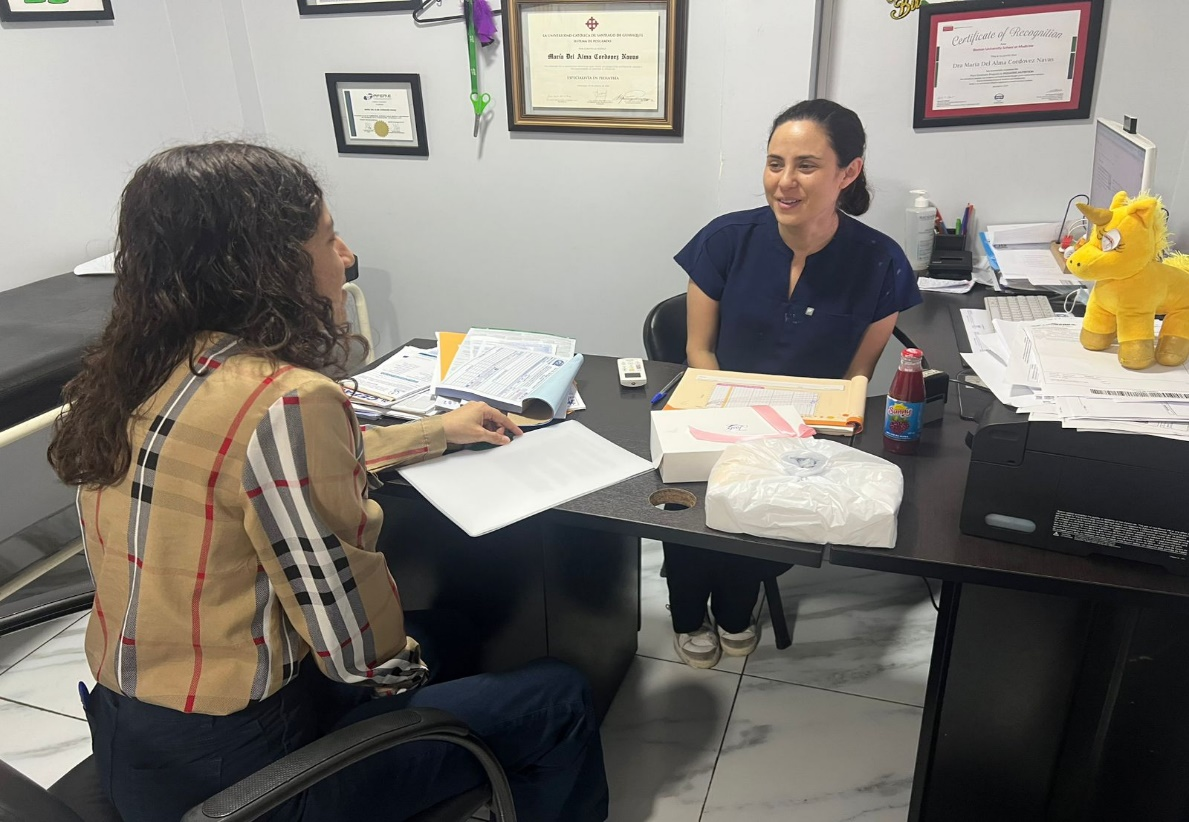
\includegraphics[width=0.8\textwidth]{images/image61.png}
			\end{figure}
			
	
\end{document}